% $Id: $
\documentclass[a4paper,11pt]{report}
\usepackage{a4wide}
\usepackage{tikz}
\usepackage{lscape}
\usepackage{tabularx}
\usepackage{ltablex}
\usetikzlibrary{arrows}
\usepackage[titletoc]{appendix}
\usepackage{mathrsfs}
\usepackage{enumerate}
\usepackage{mcode}
\usepackage[]{algorithm2e}
\usepackage{mathtools}
\usepackage{amsmath,amsthm,amssymb}
\usepackage{amsfonts}
% The following makes latex use nicer postscript fonts.
\usepackage{times}
\usepackage{subcaption}
\usepackage[english]{babel}
\usepackage{tikz}
%\usepackage[colorlinks,urlcolor=blue,linkcolor=blue]{hyperref}
\pagestyle{headings}
\newcommand{\upuparrow}{\mathrel{\reflectbox{\rotatebox[origin=c]{90}{$\twoheadrightarrow$}}}}
\newcommand{\downdownarrow}{\mathrel{\reflectbox{\rotatebox[origin=c]{90}{$\twoheadleftarrow$}}}}
\usepackage{vubtitlepage}
\usepackage{lmodern}
\usepackage{graphicx}
\usepackage{makeidx}
\usepackage[geometry]{ifsym}
%\usepackage[font=small,format=plain,labelfont=bf,up,textfont=it,up]{caption}
\renewcommand{\thefigure}{\thesection.\arabic{figure}}
\author{Filip Moons}
\title{Tiny Compiler}
%\theoremstyle{definition}
\newtheorem{theorem}{Theorem}[section]
\newtheorem{lemma}[theorem]{Lemma}
\newtheorem{proposition}[theorem]{Proposition}
\newtheorem{conjecture}{Conjecture}
\newtheorem{example}[theorem]{Example}
\let\oldexample\example
\renewcommand{\example}{\oldexample\normalfont}
\newtheorem{property}[theorem]{Property}
\newtheorem{definition}[theorem]{Definition}
\newtheorem{corollary}[theorem]{Corollary}
\newtheorem{remark}[theorem]{Remark}
\newtheorem{examples}[theorem]{Examples}
\newtheorem{remarks}[theorem]{Remarks}
\newtheorem{notation}[theorem]{Notation}

\setcounter{tocdepth}{5}
\newcommand{\N}{{\mathbb N}}
\newcommand{\Z}{{\mathbb Z}}
\newcommand{\Q}{{\mathbb Q}}
\newcommand{\R}{{\mathbb R}}
\newcommand{\C}{{\mathbb C}}
\newcommand{\HQ}{{\mathbb H}}
\renewcommand{\P}{{\mathbb P}}
\newcommand{\E}{{\mathbb E}}
\newcommand{\cost}{\text{cost}}
\newcommand{\Nash}{\text{Nash}}
\newcommand{\nash}{\text{nash}}
\newcommand{\opt}{\text{opt}}
\newcommand{\LFP}{\text{LFP}}
\renewcommand{\int}{\text{int}}
\newcommand{\graf}{\mathscr{G}}
\newcommand{\grafeen}{\mathscr{H}}
\newcommand{\hgraf}{\mathcal{G}}
\usepackage{eufrak}
\newcommand{\hgrafeen}{\mathcal{H}}
\newcommand{\vect}{\operatorname{vec}}
\newcommand{\tol}{\text{TOL}}

%\newenvironment{proof}{\noindent{\bf Bewijs.}}{{\hfill $ \ Box $}\vskip 4mm}

\promotortitle{Promotor}
\promotor{Prof. Dr. P. Cara}
\advisors{}
\author{Filip Moons}
\title{Similarity on Graphs \& Hypergraphs}
\advisortitle{}
\date{MEI 2006}
\faculty{Faculty of Science}
\advisortitle{}
\department{Master in Mathematics - specialization: Education}
\reason{Graduation thesis submitted in partial fulfillment of the requirements
for\\ the degree of Master of Science in Mathematics - specialization: Education}

\date{June 2015}


\begin{document}
% Then english TitlePage
\maketitlepage
\chapter*{Acknowledgements}
First of all, I would like to thank my promotor, Philippe Cara for his incredible attention to detail, 
for the patience he had with me and the many reminders to continue and to work 
hard. He also showed me the way to this beautiful topic for a Master thesis. Besides his role as 
promotor, I will never forget him as professor of the Linear Algebra course in 
the very first term of the BSc in Mathematics, that without any doubt was the 
most memorable course during my college years: the hard study and the stress I 
had before entering the exam room are memories that I still will be telling in my old age.

Secondly, I would like to thank Roger Van Nieuwenhuyze, my math lecturer during 
the teacher training I followed for one year at the Hogeschool-Universiteit Brussel. Without his encouragements, I had never dared to leave
and study Mathematics at university level. 

I also want to thank all professors and teaching assistant who have learned me a 
lot during the past five years. A special thanks goes to Reen Tallon, who 
always managed to overcome any administrative burden caused by the combination 
of programs.

Last but not least, I want to thank my parents for their angry looks when they 
felt I did not study enough, it certainly kept me on track. Also my partner Sacha and my friends from university and the Classical Liberal Student  
Union made my college years unforgettable for the rest of my life.


 
\chapter*{Abstract}


\chapter*{Samenvatting}
Deze thesis bespreekt similariteit op graffen \& hypergraffen. De notie van 
similariteit op graffen vindt zijn oorsprong in het HITS-algoritme: dit algoritme 
werd eind jaren negentig ontdekt om zoekresultaten van een internetzoekmachine op een betekenisvolle manier 
te sorteren. Het algoritme onderzoekt de relaties tussen de hyperlinks van een verzameling webpagina's: sommige webpagina's worden 
bestempeld als goede doorverwijzers, andere webpagina's worden dan weer als een gezaghebbende bron beschouwd voor de zoekterm. 
Uiteraard is deze tweedeling sterk verwant: pagina's die goede doorverwijzers 
zijn zullen veel links naar pagina's bevatten die als een gezaghebbende bron 
gezien worden en omgekeerd, zullen pagina's als gezaghebbende bron worden 
beschouwd als ze veel inkomende links krijgen van goede doorverwijzers. Dit 
algoritme was erg vernieuwend in die tijd, vermits tot dan toe zoekresultaten 
enkel gesorteerd werden op het aantal inkomende links (zonder daarbij de bronpagina na te gaan) 
of het aantal keren dat een zoekterm voorkwam.

Deze methode werd rond 2005 veralgemeend naar een notie van similariteit tussen 
graffen. Een verzameling webpagina's die onderling gelinkt zijn zoals die in het HITS-algoritme gebruikt worden,
kan immers beschouwd worden als een graf. Deze veralgemening leidt tot een 
methode waarbij we een soort score kunnen kleven op hoe twee toppen van twee verschillende graffen op elkaar lijken. 
Deze `similariteisscore' zal hoger zijn als de adjacente toppen van deze twee toppen 
ook gelijkaardig zijn.

Eens we similariteit op de toppen van graffen hebben ingevoerd, gaan we deze 
methode verder uitbreiden tot similariteit op toppen en bogen van graffen en tot 
similariteit tussen gekleurde graffen. We hebben zo een compleet overzicht van 
de meest recente studies over het onderwerp. Opvallend is dat de convergentie van de resulterende algoritmes van al deze uitbreidingen met 
dezelfde convergentiestelling kunnen bewezen worden.

Een belangrijke opmerking is hier wel dat deze verschillende uitbreidingen lichtjes 
andere resultaten opleveren. Er bestaat niet zoiets als `de' similariteitsscore tussen twee 
toppen van twee graffen, eenvoudigweg omdat elke uitbreiding een licht verschillend resultaat zal opleveren.
Daarom zijn deze similariteitscores vooral in verhouding tot de andere scores interessant: we kunnen 
bv. gemakkelijk bepalen welke top van de ene graf, het meest lijkt op de top van een andere 
graf simpelweg door de grootste similariteitsscore te bekijken.    Dit zal ook blijken uit het korte overzicht van toepassingen dat op 
het einde van deze masterproef is toegevoegd, ook daar wordt een
similariteitsscore enkel in verhouding tot de andere similareitsscores bekeken.

In het voorlaatste hoofdstuk ontdekken we tot slot nieuw terrein: we proberen 
via tensoren het concept van similariteit over te brengen op de meer algemene 
structuur van hypergraffen. Een generalizatie die wonderwel slaagt door de tensoren zo om te vormen dat we opnieuw dezelfde convergentiestelling als bij graffen toe te 
passen. Toch is er ook een grote maar, want net zoals bij de meeste andere
uitbreidingen via tensoren, is ook hier de vloek van de dimensionaliteit nooit ver weg. 


 

\tableofcontents
\newpage
% \pagenumbering{arabic}
\chapter{Preliminaries and notations}


The Perron-Frobenius theorem states that a real square matrix with nonnegative entries has a unique largest real eigenvalue with an eigenvector 
that has only positive entries. The theorem was proved by Oskar 
Perron (1880-1975) in 1907 for strictly positive entries and extended by 
Ferdinand Georg Frobenius (1849-1917) to irreducible matrices with nonnegative 
entries. 

\section{Some families of matrices}
In this section, we first introduce different kinds of matrices. Note that all matrices in this master thesis have real entries,
unless otherwise stated. We start with permutation matrices and their uses. 
With permutation matrices, we can introduce irreducible matrices. Also nonnegative and primitive square matrices are presented. After defining 
those, we look at the Perron-Frobenius theorem. 
\subsection{Permutation matrices}
\begin{definition}\label{petmruation}
  Given a permutation $\pi$ of $n$ elements:
  $$\pi: \{1,\ldots,n\} \to \{1,\ldots,n\},$$
  with:
    $$\pi = \begin{pmatrix} 1 & 2 & \cdots & n \\ \pi(1) & \pi(2) & \cdots & \pi(n) \end{pmatrix} $$
  the associated \textbf{permutation matrix} $P_\pi$ is the $n\times n$-matrix 
  obtained by permuting the rows of the identity matrix $I_n$ according to $\pi$. 
  So:
 $$P_\pi = \begin{bmatrix} 
e^T_{\pi(1)}  \\
e^T_{\pi(2)}  \\
\vdots  \\
e^T_{\pi(n)}  
\end{bmatrix}.$$
 where $e_{j}$ is the $j$-th column of $I_n$.
 \end{definition}
\begin{example}
  The permutation matrix $P_\pi$ corresponding to the permutation  $$\pi = \begin{pmatrix} 1 & 2 & 3 & 4 \\ 1 & 4 & 2 & 3 \end{pmatrix} $$
  is:
  $$P_\pi = \begin{bmatrix} 
1 & 0 & 0 & 0  \\
0 & 0 & 0 & 1  \\
0 & 1 & 0 & 0  \\
0 & 0 & 1 & 0  
\end{bmatrix}.$$
Note that $p_{ij} = 1$ if and only if $\pi(i) = j$. 
\end{example}

\begin{property}\label{permutatie}
A permutation matrix $P$ satisfies:
  $$PP^T = I_n,$$
  where $P^T$ is the transpose and $I_n$ is the identity matrix.
\end{property}
\begin{proof}
By direct computation, we get:
$$(PP^T)_{ij} = \sum^n_{k=1}P_{ik}P^T_{kj} = \sum^n_{k=1}P_{ik}P_{jk}$$
Assume $i \not = j$. Then for each $k$, $P_{ik}P_{jk} = 0$ since there is only
one nonzero entry in the $k$-th row and $i \not = j$, $P_{ik}$ and $P_{jk}$ 
can't be both the nonzero entry. So, $(PP^T)_{ij} = 0$ when $i \not = j$.

When $i=j$, then there exists a $k' \in \{1,\ldots,n\}$ with $P_{ik'}P_{jk'} = 1$, 
since there is only one nonzero entry in the $k$-th row, this $k'$ is unique, 
which results in $\sum^n_{k=1}P_{ik}P_{jk} = (PP^T)_{ij} = 1$.

In other words,
$$(PP^T)_{ij} = \begin{cases} 1 &\mbox{if } i = j \\ 
0 & \mbox{otherwise} \end{cases},$$
this is exactly the formula for the entries of the identity matrix.
\end{proof}

\begin{corollary}
  The transpose of a permutation matrix $P$ is its inverse:
  $$P^T = P^{-1}.$$
  This can also more easily be concluded by the fact that a permutation matrix 
  is clearly an orthogonal matrix (a real $n \times n$-matrix with orthonormal 
  entries).
\end{corollary}
\subsection{Nonnegative and primitive matrices}
\begin{definition}\label{groterkleiner}
  Let $A$ and $B$ be two real $n\times r$-matrices. Then, $A \geq B$ (respectively $A > B$) if $a_{ij} \geq b_{ij}$ 
  (respectively $a_{ij}>b_{ij}$) for all $1 \leq i \leq n, 1 \leq j\leq r$. 
\end{definition}
\begin{definition}  A real $n\times r$-matrix $A$ is \textbf{nonnegative} if $A \geq 0$, with $0$ the $n\times r$-null matrix.
\end{definition}
\begin{definition}  A real $n\times r$-matrix $A$ is \textbf{positive} if $A > 0$, with $0$ the $n\times r$-null matrix.
\end{definition}

Since row vectors are $1 \times n$-matrices, we shall use the terms 
nonnegative and positive vector throughout. 

\begin{notation}\label{modulusmatrix}
  Let $B$ be an arbitrary complex $n\times r$-matrix, then $|B|$ denotes the 
  matrix with entries $|b_{ij}|$. This is not to be confused with the 
  determinant of a square matrix $B$, which we denote by $\det(B)$.
\end{notation}

\begin{definition}  A nonnegative square matrix $A$ is called \textbf{primitive} if there is a $k \in \N_0$ such that all entries of $A^k$ are positive.
 \end{definition}

\subsection{Irreducible nonnegative matrices}
In developing the Perron-Frobenius theory, we shall first establish a series of 
theorems and lemmas on nonnegative irredicuble square matrices. 
\begin{definition}\label{defreduciebel} A square matrix $A$ is called \textbf{reducible} if there is a permutation matrix $P$ such that 
 $$PAP^T = \begin{pmatrix}  B  & 0\\
 C  & D\\
\end{pmatrix} $$
where $B,$ and $D$ are square matrices, each of size at least one and $0$ is a zero matrix.
A square matrix $A$ is called \textbf{irreducible} if it is not reducible.
 \end{definition}
It follows immediately that a $1\times1$-matrix is always irreducible by 
definition. We now show a useful property to identify a reducible matrix.
\begin{property}\label{propertyreducible}
  Let $A$ be an $n\times n$-matrix with $n\geq 2$. Consider a nonempty, proper subset $S$ of $\{1,\ldots,n\}$ with 
  $a_{ij}=0$ for $i \in S$, 
  $j \not\in S$. Then A is  reducible.
\end{property}
\begin{proof}
  Let $S=\{i_1, i_2,\ldots, i_k\}$, where we assume, without loss of generality, 
  that $i_1 < i_2 < \cdots < i_{k-1} < i_k$. Let $S^c$ be the complement of $S$, consisting of the
  ordered set of elements $j_1 < j_3 < \cdots < j_{n-k}$. Consider the permutation $\sigma$ of
  $\{1,2,\ldots,n\}$ given by
  $$\sigma = \begin{pmatrix} 1 & 2 & \ldots & k & k + 1 & k+ 2 & \ldots & n \\ 
  i_1 & i_2 & \ldots & i_k & j_1 & j_2 & \ldots & j_{n-k} \end{pmatrix} $$

$\sigma$ can be represented by the permutation matrix $P_\sigma = (p_{ij})$, 
where $p_{rs} = 1$ if $\sigma(r) = s$. We prove that
 $$PAP^T = \begin{pmatrix}  B  & 0\\
 C  & D\\
\end{pmatrix} $$

where $B$ and $D$ are square matrices and $0$ is a $k \times (n-k)$ zero matrix. 
Consider row $c$ and column $d$, where $1 \leq c \leq k$ and $k + 1 \leq d \leq
n$:
\begin{eqnarray}\label{redenering1}
(PAP^T)_{cd} = \sum_i\sum_j p_{c i}a_{ij}p_{d j}.
\end{eqnarray}
It is enough to show that each term in the summation is zero. Suppose $p_{c i} =
p_{d j} = 1$. Thus $\sigma(c) = i$ and $\sigma(d)= j.$ Since $1 \leq c \leq
k$, then $i \in \{i_1, i_2,\ldots, i_k\}$; similarly, since $k+1 \leq d \leq n$, we have $j \in 
\{j_1,j_2,\ldots,j_{n-k}\}.$ By assumption, for such a pair $i, j$, we have $a_{ij}=0$. That completes
the proof. 
\end{proof}
We know prove some equivalent definitions for a nonnegative, irreducible square 
matrix.
\begin{theorem}\label{irredubieleegenschappen}
  Let $A\geq 0$ be a nonnegative $n\times n$-matrix. Then the following conditions are 
  equivalent:
  \begin{enumerate}
    \item[(1)] $A$ is irreducible.
    \item[(2)] $(I + A)^{n-1} > 0$
   \item[(3)] For any pair $(i,j)$, with $1 \leq i, j \leq n$, there is a 
   positive integer $k = k(i,j) \leq n$ such that $(A^k)_{ij} > 0$.
  \end{enumerate}
\end{theorem}
\begin{proof}
  
  $(1) \Rightarrow (2)$: Let $\mathbf{x} \geq 0, \mathbf{x} \not = \mathbf{0}$ be an arbitrary vector in $\R^n$.
  If a coordinate of $\mathbf{x}$ is positive, the same coordinate is positive  in $\mathbf{x} + A\mathbf{x} = (I+A)\mathbf{x}$ 
  as well. We claim that $(I+A)\mathbf{x}$ has fewer zero coordinates than 
  $\mathbf{x}$ as long as $\mathbf{x}$ has a zero coordinate. If this claim is 
  not true, then the number of zero coordinates must be at least equal,
  this means that for each coordinate $j$ with $x_j = 0$ we would have that $x_j+ (A\mathbf{x})_j= 0$. Let $J = \{j: x_j > 0\}.$ For any $j \not \in J, r\in J$, we have 
  $(A\mathbf{x})_j = \sum_k a_{jk}x_k = 0$ and $x_r > 0$. 
  It must be that $a_{jr} = 0$. It follows from Property \ref{propertyreducible} that $A$ 
  is reducible, which is a contradiction and the claim is proved. Thus $(I+A)\mathbf{x}$ 
  has at most $n-2$ zero coordinates. Continuing in this manner we conclude that 
  $(I + A)^{n-1}\mathbf{x} > 0$. Let $\mathbf{x} = \mathbf{e}_i$, then the corresponding column of $(I+A)^{n-1}$ must be 
  positive. Thus (2) holds.
  
  $(2) \Rightarrow (3)$: We have $(I + A)^{n-1} > 0$, $A \geq 0$, so $A \not = 0$ 
  and 
  $$A(I+A)^{n-1} = \sum_{k=1}^n {n-1 \choose k-1} A^k > 0.$$
Thus for any $i, j$ at least one of the matrices $A, A^2,\ldots, A^n$ has its 
$(i,j)$-th element entry positive.

$(3) \Rightarrow (1)$: Suppose $A$ is reducible. Then for some permutation 
matrix $P$,
$$PAP^T = \begin{pmatrix}  B_1  & 0\\
 C_1  & D_1\\
\end{pmatrix} $$
where $B_1$ and $D_1$ are square matrices. Furthermore, we know from Property \ref{permutatie} that 
$PAP^TPAP^T = PA^2P^T$,
whence for some square matrices $B_2, C_2$ we have:
$$PA^2P^T = \begin{pmatrix}  B_2  & 0\\
 C_2  & D_2\\
\end{pmatrix} $$
More generally, for some matrix $C_t$ and square matrices $B_t$ and $D_t$,
$$PA^tP^T = \begin{pmatrix}  B_t  & 0\\
 C_t & D_t\\
\end{pmatrix} $$
Thus $(PA^tP^T)_{rs} = 0$ for $t = 1, 2,\ldots$ and for any $r,s$ 
corresponding to an entry of the zero submatrix in $PAP^T$.
Now, for $t = 1,\ldots,n:$
$$0 = (PA^tP^T)_{rs} = \sum_k\sum_l p_{r k}a_{kl}^{(t)}p_{s t}$$
By using the same reasoning as in \ref{redenering1}, choose $k,l$ so that $p_{r k}$ = $p_{s t} = 1$. Then $a^{(t)}_{kl} = 0$ for all $t$,
contradicting the hypothesis. This completes the proof. 
 \end{proof}
 
 
 \begin{corollary}
   If $A$ is irreducible then $I+A$ is primitive. 
 \end{corollary}
 \begin{corollary}
   $A^T$ is irreducible whenever $A$ is irreducible.
 \end{corollary}
 \begin{property}\label{geenzerorij}
  No row or column of an irreducible matrix $A$ can vanish. This means that $A$ cannot have a row or a column of zeros.
   \end{property}
 \begin{proof}
   Suppose that $A$ has a zero row, then it could be permuted to
     $$PAP^T = \begin{pmatrix}  0 & 0 \ldots 0\\
\begin{tabular}{l}
c_1  \\
\vdots \\
c_n\\   
\end{tabular}
 & D\\
 \end{pmatrix} $$
 by some permutation matrix $P$. It follows from Definition \ref{defreduciebel} 
 that $A$ is reducible. Similarly, if $A$ has zero column, it can be permuted 
 to
   $$PAP^T = \begin{pmatrix} B & \begin{tabular}{l}
0 \\
\vdots \\
0\\   
\end{tabular}\\
    c_1  \ldots c_n   & 0\\
    \end{pmatrix} $$
    again from Definition \ref{defreduciebel} we conclude that $A$ is reducible.

 \end{proof}
 
 

 \section{Perron-Frobenius Theorem}
 
 \subsection{Spectral radii of nonnegative matrices}
 
 \begin{definition}
  Let A be an $n\times n$-matrix with complex entries and eigenvalues $\lambda_i$,
  $1 \leq i \leq n$. Then:
  $$\rho(A) = \max_{1 \leq i \leq n} |\lambda_i|$$
  is called the \textbf{spectral radius} of the matrix $A$.
\end{definition}

Geometrically, if all the eigenvalues $\lambda_i$ of $A$ are plotted in the 
complex plane, then $\rho(A)$ is the radius of the smallest disk $|z| \leq 
R$, with center at the origin, which includes all the eigenvalues of the matrix 
$A$.

 We now establish a series of lemmas on nonnegative irreducible square matrices. 
 These lemmas will allow us to prove the Perron-Frobenius at the end of this
 section.\\
 
 If $A \geq 0$ is an irreducible $n\times n$-matrix and $\mathbf{x}$, a vector of size $n$ with $\mathbf{0} \not = \mathbf{x} \geq 0$, let
 \begin{eqnarray}
r_\mathbf{x} = \min\left\{\frac{\sum^n_{j=1}a_{ij}x_j}{x_i}\right\}
  \end{eqnarray}
 where the minimum is taken over all $i$ for which $x_i > 0$. Clearly, $r_\mathbf{x}$ is 
 a nonnegative real number and is the supremum of all $p \geq 0$ for 
 which 
  \begin{eqnarray}\label{eenvoudigefrob}
A\mathbf{x} \geq p\mathbf{x}  \end{eqnarray}
 
  We now consider the nonnegative quantity $r$ defined by 
 \begin{eqnarray}\label{eenvoudigefrob2}\label{quantityr}
   r = \sup_{\begin{subarray}{l}\mathbf{x} \geq 0\\
    \mathbf{x}\not = \mathbf{0}\end{subarray}} \{r_\mathbf{x}\}
 \end{eqnarray}
As $r_{\mathbf{x}}$ and $r_{\alpha\mathbf{x}}$ 
have the same value for any 
scalar $\alpha > 0$, we need consider only the set $B$ of vectors $\mathbf{x} \geq 0$ 
with $||\mathbf{x}|| = 1$, and we correspondingly let $Q$ be the set of all vectors $\mathbf{y}=(I+A)^{n-1}\mathbf{x}$ 
where $\mathbf{x} \in B$. From Theorem \ref{irredubieleegenschappen} , $Q$ 
consists only of positive vectors. Multiplying both sides of the inequality $A\mathbf{x} \geq r_{\mathbf{x}}\mathbf{x}$
by $(I+A)^{n-1}$, we obtain:

$$\forall \mathbf{y} \in Q: A\mathbf{y} \geq r_{\mathbf{x}}\mathbf{y},$$
and we conclude from (\ref{eenvoudigefrob}) that $r_\mathbf{y} \geq 
r_{\mathbf{x}}$. Therefore, the quantity $r$ of (\ref{eenvoudigefrob2}) can be 
defined equivalently as:
\begin{eqnarray}\label{quantityr2}
  r = \sup_{\mathbf{y} \in Q} \{r_{\mathbf{y}}\}
\end{eqnarray}
As $B$ is a compact set (in the usual topology) of vectors, so is $Q$, and as $r_\mathbf{y}$ is a continuous 
function on $Q$, we know from the extreme value theorem that there necessarily exists a positive vector $\mathbf{z}$ for which:
\begin{eqnarray}\label{frobbrol3}
  A\mathbf{z} \geq r\mathbf{z},
 \end{eqnarray}
 and no vector $\mathbf{w} \geq 0$ exists for which $A\mathbf{w} > r\mathbf{w}$. 
\begin{definition}
  We call all nonnegative, nonzero vectors $\mathbf{z}$ satisfying 
  (\ref{frobbrol3})
  \textbf{extremal vectors} of the matrix $A$.
\end{definition}

\begin{lemma}
  If $A \geq 0$ is an irreducible $n\times n$-matrix, the quantity $r$ of (\ref{quantityr}) 
  is positive.
\end{lemma}
\begin{proof}
  If $\mathbf{x}$ is the positive vector whose coordinates are all unity, then since the matrix $A$ is irreducible, 
  we know from Property \ref{geenzerorij} that no row of $A$ can vanish, and consequently no component of $A\mathbf{x}$ 
  can vanish. Thus, $r_\mathbf{x} > 0$, proving that $r > 0$.
  \end{proof}
  
  \begin{lemma}\label{lemmafrobextremal} If $A \geq 0$ is an irreducible $n\times n$-matrix, each extremal vector $\mathbf{z}$ is a positive 
  eigenvector of $A$ with corresponding eigenvalue $r$ of (\ref{quantityr}), i.e., $A\mathbf{z} 
  = r\mathbf{z}$ and $\mathbf{z} > 0$.
  \end{lemma}
  \begin{proof}
    Let $\mathbf{z}$ be an extremal vector with $A\mathbf{z} - r \mathbf{z}= 
    \mathbf{t}$. If $\mathbf{t}\not = \mathbf{0}$, then some coordinate of $\mathbf{t}$ is 
    positive; multiplying through by the matrix $(I+A)^{n-1}$, we have:
    $$A\mathbf{w} - r\mathbf{w} > 0, \text{ with } \mathbf{w} = (I+A)^{n-1}\mathbf{z}$$
    from Theorem \ref{irredubieleegenschappen} we know that $\mathbf{w} > 0$. It 
    would then follow that $r_{\mathbf{w}} > r$, contradicting the definition of 
    $r$ in (\ref{quantityr2}). Thus $A\mathbf{z} = r\mathbf{z}$, and since 
    $\mathbf{w} > 0$ and $\mathbf{w} = (1+r)^{n-1}\mathbf{z}$, then we have $\mathbf{z} 
    > 0$, completing the proof.
  \end{proof}
  
  \begin{lemma}\label{lemma2frobvolledig}
    Let $A \geq 0$ be an irreducible $n\times n$-matrix, and let $B$ be an $n\times 
    n$- complex matrix with $|B|\leq A$. If $\beta$ is any eigenvalue of $B$, 
    then 
\begin{eqnarray}\label{lemma2frob}
|\beta| \leq r,  
\end{eqnarray}
where $r$ is the positive quantity of (\ref{quantityr}). Moreover, equality is 
valid in (\ref{lemma2frob}), i.e., $\beta = re^{i\phi}$, if and only if $|B| = 
A$, and where $B$ has the form:
\begin{eqnarray}\label{lemma2frobvormB}
B = e^{i\phi}DAD^{-1},
\end{eqnarray}
and $D$ is a diagonal matrix whose diagonal entries have modulus unity.
  \end{lemma}
  
  
  \begin{proof}
  If $\beta\mathbf{y} = B\mathbf{y}$ where $\mathbf{y} \not = \mathbf{0}$, then
  $$\beta y_i = \sum_{j=1}^n b_{ij}y_i, \text{ with } 1 \leq i \leq n.$$
  Using the hypotheses of the lemma and the notation of Definition \ref{modulusmatrix}, it follows that:
  \begin{eqnarray}
|\beta||\mathbf{y}| \leq |B||\mathbf{y}| \leq A |\mathbf{y}|,
\end{eqnarray}
which implies that $|\beta| \leq r_{|\mathbf{y}|} \leq r$, proving 
(\ref{lemma2frob}). If $|\beta| = r$, then $|\mathbf{y}|$ is an extremal vector 
of $A$. Therefore, from Lemma \ref{lemmafrobextremal}, $|\mathbf{y}|$ is a 
positive eigenvector of $A$ corresponding to the positive eigenvalue $r$. Thus,
\begin{eqnarray}\label{lemma2frobconclusion}
  r|\mathbf{y}| = |B||\mathbf{y}| = A|\mathbf{y}|,
\end{eqnarray}
and since $|\mathbf{y}| > 0$, we conclude from (\ref{lemma2frobconclusion}) and 
the hypothesis $|B| \leq A$ that 
\begin{eqnarray}\label{lemma2frobBeqA}  |B| = A
  \end{eqnarray}
For the vector $\mathbf{y}$, where $|\mathbf{y}| > 0$, let
$$D = \text{diag}\left\{\frac{y_1}{|y_1|}, \ldots, \frac{y_n}{|y_n|}\right\}.$$
It is clear that the diagonal entries of $D$ have modulus unity, and
\begin{eqnarray}
  \mathbf{y} = D|\mathbf{y}|.
    \end{eqnarray}
Setting $\beta = re^{i\phi}$, then $B\mathbf{y} = \beta\mathbf{y}$ can be 
written as:
\begin{eqnarray}\label{lemma2frobC}
  C|\mathbf{y}| = r|\mathbf{y}|,
\end{eqnarray}
where
\begin{eqnarray}\label{lemma2frobdefC}
  C = e^{-i\phi}D^{-1}BD.
\end{eqnarray}
From (\ref{lemma2frobconclusion}) and (\ref{lemma2frobC}), equiting terms equal 
to $r|\mathbf{y}|$ we have
\begin{eqnarray}\label{lemma2frobequalsmatriceswithy}
 C|\mathbf{y}| = |B||\mathbf{y}| = A|\mathbf{y}|.
 \end{eqnarray}
 From the definition of the matrix $C$ in (\ref{lemma2frobdefC}), $|C| = |B|$. 
 Combining with (\ref{lemma2frobBeqA}), we have:
 \begin{eqnarray}\label{lemma2frobequalsmatrices}
 |C| = |B| = A.
 \end{eqnarray}
 Thus, from (\ref{lemma2frobequalsmatriceswithy}) we conclude that $C|\mathbf{y}| = 
 |C||\mathbf{y}|$, and as $|\mathbf{y}| > 0$, it follows that $C = |C|$ and thus $C = A$ from  
 (\ref{lemma2frobequalsmatrices}). Combining this result with 
 (\ref{lemma2frobdefC}), gives the desired result that $B = e^{i\phi}DAD^{-1}$. 
 Conversely, it is obvious that if $B$ has the form in (\ref{lemma2frobvormB}), 
 then $|B|=A$, and $B$ has an eigenvalue $\beta$ with $|\beta| = r$, which 
 completes the proof.
\end{proof}

\begin{corollary}\label{lemma2frobcorollary}
  If $A \geq 0$ is an irreducible $n\times n$-matrix, then the positive 
  eigenvalue $r$ of Lemma \ref{lemmafrobextremal} equals the spectral radius $\rho(A)$ 
  of $A$
\end{corollary}  
\begin{proof}
  Setting $B = A$ in Lemma \ref{lemma2frobvolledig} immediately gives us this
  result.
\end{proof}
 In other words, if $A \geq 0$ is an irreducible $n\times n$-matrix, its 
 spectral radius $\rho(A)$ is positive, and the intersection in the complex 
 plane of the circle $|z| = \rho(A)$ with the positive real axis is an 
 eigenvalue of $A$.
 \begin{definition}
   A \textbf{principal square submatrix} of an $n\times n$-matrix A is any 
   matrix obtained by crossing out any $j$ rows and the corresponding $j$
 columns of $A$, with $1 \leq j \leq n.$ \end{definition}
 \begin{lemma}\label{froblemma4}
   If $A \geq 0$ is an irreducible $n\times n$-matrix, and $B$ is any principal 
   square submatrix of $A$, then $\rho(B) < \rho(A).$
 \end{lemma}
 \begin{proof}
   If $B$ is any principal submatrix of $A$, then there is an $n\times 
   n$-permutation matrix $P$ such that $B = A_{11}$ where
   \begin{eqnarray}
    C = \begin{pmatrix}  A_{11}  & 0\\
 0  & 0\\
\end{pmatrix};
PAP^T =  \begin{pmatrix}  A_{11}  & A_{12}\\
 A_{21}  & A_{22}\\
\end{pmatrix}
  \end{eqnarray}
Here, $A_{11}$ and $A_{22}$ are, respectively, $m\times m$ and $(n-m) \times (n-m)$ 
principal square submatrices of $PAP^T$, $1 \leq m \leq n.$ Clearly, $0\leq C \leq 
PAP^T$, and $\rho(C) = \rho(B) = \rho(A_{11})$, but as $C = |C| \not = PAP^T$, 
the conclusion follows immediately from Lemma \ref{lemma2frobvolledig} and 
Corollary \ref{lemma2frobcorollary}.
 
  \end{proof}


   The following lemma is used to prove that $\rho(A)$ is a simple 
   eigenvalue of $A$ in the Perron-Frobenius theorem. The proof uses the 
   extension of the product rule of derivation for multilinear functions 
   $M(a_1,\ldots,a_k)$. Suppose $x_1,..,x_k$ are differentiable vector functions, 
   then $M(x_1,\ldots,x_k)$ is differentiable and:
   $$\frac{\mathrm{d}}{\mathrm{d}t}M(x_1,\ldotsx_k) = M(\frac{\mathrm{d}}{\mathrm{d}t} x_1, x_2, \ldots, x_k) 
   + M(x_1, \frac{\mathrm{d}}{\mathrm{d}t} x_2, \ldots, x_k) + \ldots +  M(x_1,  x_2, \ldots,\frac{\mathrm{d}}{\mathrm{d}t} x_k) $$
   The most important application of this rule is for the derivative of the determinant:
   $$\frac{\mathrm{d}}{\mathrm{d}t}\det(x_1,\ldots, x_k) = \det(\frac{\mathrm{d}}{\mathrm{d}t} x_1, x_2, \ldots, x_k) 
   + \det(x_1, \frac{\mathrm{d}}{\mathrm{d}t} x_2, \ldots, x_k) + \ldots + \det(x_1,  x_2, \ldots,\frac{\mathrm{d}}{\mathrm{d}t} x_k) $$

 \begin{lemma}\label{maclane}

   Let $A$ be an $n \times n$-matrix over the complex numbers and let $\phi(A, \lambda) = \det(\lambda I_n - A)$
   be the characteristic polynomial of $A$. Let $B_i$ be the principal submatrix 
   of $A$ formed by deleting the $i$-th row and column of $A$ and let $\phi(B_i, \lambda)$ 
   be the characteristic polynomial of $B_i$. Then:
   $$\phi'(A, \lambda) = \frac{\mathrm{d}\phi(A, \lambda)}{\mathrm{d}\lambda}= 
   \sum_i \phi(B_i, \lambda)$$
 \end{lemma}
\begin{proof}
  The proof is immediately done by direct computation:
  
  $$\phi(A, \lambda) = \det\begin{bmatrix} 
\lambda -a_{1,1} & -a_{1,2}  & \ldots & -a_{1,n}   \\
-a_{2,1}  & \lambda - a_{2,2} & \ldots & -a_{2,n}   \\
\vdots & \vdots & \ddots & \vdots  \\
- a_{n,1}  & -a_{n,2} & \ldots & \lambda - a_{n,n}  
\end{bmatrix}.$$
Using the extension of the product rule of derivation for multilinear functions
\begin{eqnarray*}
  \phi'(A, \lambda) = \det\begin{bmatrix} 
1 & 0  & \ldots & 0    \\
-a_{2,1}  & \lambda - a_{2,2} & \ldots & -a_{2,n}   \\
\vdots & \vdots & \ddots & \vdots  \\
- a_{n,1}  & -a_{n,2} & \ldots & \lambda - a_{n,n}  
\end{bmatrix} + 
\det\begin{bmatrix} 
\lambda -a_{1,1} & -a_{1,2}  & \ldots & -a_{1,n}   \\
0  & 1 & \ldots &  0   \\
\vdots & \vdots & \ddots & \vdots  \\
- a_{n,1}  & -a_{n,2} & \ldots & \lambda - a_{n,n}  
\end{bmatrix} + \ldots \\
+ \det\begin{bmatrix} 
\lambda -a_{1,1} & -a_{1,2}  & \ldots & -a_{1,n}   \\
-a_{2,1}  & \lambda - a_{2,2} & \ldots & -a_{2,n}   \\
\vdots & \vdots & \ddots & \vdots  \\
0  & 0 & \ldots & 1
\end{bmatrix} = \sum_i \phi(B_i, \lambda).
\end{eqnarray*}
\end{proof}
\subsection{Proof}
We now collect the above results into the following main theorem: we finally 
arrived at the Perron-Frobenius Theorem:
\begin{theorem}(\textbf{Perron-Frobenius theorem})\label{frobtheorem}
  Let $A \geq 0$ be an irreducible $n\times n$-matrix. Then,
  \begin{enumerate}
    \item $A$ has a positive real eigenvalue equal to its spectral radius.
    \item To $\rho(A)$ there corresponds an eigenvector $\mathbf{x} > 0$.
    \item $\rho(A)$ increases when any entry of $A$ increases.
    \item $\rho(A)$ is a simple eigenvalue of $A$.
    \item If $A\mathbf{x} = \rho(A)\mathbf{x}$ where $\mathbf{x} > 0$ and $\mathbf{x}$ 
    is a normalized vector, then $\mathbf{x}$ is unique.
    
  \end{enumerate}
  \end{theorem}
 \begin{proof}
  (1) and (2) follow immediately from Lemma \ref{lemmafrobextremal} and 
   Corollary \ref{lemma2frobcorollary}. 
   
  (3) Suppose we increase 
   some entry of the matrix $A$, giving us a new irreducible matrix $\tilde{A}$ 
   where $\tilde{A} \geq A$ and  $\tilde{A} \not = A$. Applying Lemma 
   \ref{lemma2frobvolledig}, we conclude that $\rho(\tilde{A}) > \rho(A).$ 
   
   (4) $\rho(A)$ is a simple eigenvalue of $A$, i.e., $\rho(A)$ is a zero of multiplicity one of the characteristic polynomial
   $\phi(\lambda) = \det(\lambda I_n - A)$, we make use of Lemma \ref{maclane} by using the fact that $\phi'(\lambda)$ is the sum of the
   determinants of the principal $(n-1)\times(n-1)$ submatrices of $\lambda I - A$. If $A_i$ is any principal submatrix of
   $A$, then from Lemma \ref{froblemma4}, $\det(\lambda I - A_i)$ (with $I$ the identity matrix with the same size as the principal submatrix $A_i$) cannot vanish 
   for any $\lambda \geq \rho(A)$. From this it follows that:
   $$\det(\rho(A)I - A_i) > 0,$$
   and thus
   $$\phi'(\rho(A)) > 0.$$
   Consequently, $\rho(A)$ cannot be z zero of $\phi(\lambda)$ of multiplicity 
   greater than one and thus $\rho(A)$ is a simple eigenvalue of $A$. 
   
  (5) If $A\mathbf{x} = \rho(A)\mathbf{x}$ where $\mathbf{x} > 0$ 
   and $||x|| = 1$ ($||x||$ denotes the standard Euclidean norm), we cannot find 
   another eigenvector $\mathbf{y} \not = s\mathbf{x}$, with $s$ a scalar, of $A$ 
   with $A\mathbf{y} = \rho(A)\mathbf{y}$, so that the eigenvector $\mathbf{x}$ 
   , meaning that the normalized eigenvector $\mathbf{x}$ is uniquely 
   determined.
       \end{proof}

   
   With the previous proof in mind, the following definition comes not unexpected:
   
   \begin{definition}\label{perronroot}
     If a matrix $A$ has an eigenvalue equal to the spectral radius $\rho(A)$, this eigenvalue
     is called the \textbf{Perron root}, the corresponding eigenvector $\mathbf{x}$ such that:
     $$A\mathbf{x} = \rho(A)\mathbf{x} \quad \text{and} \quad \|\mathbf{x}\|_1 = 1$$s called 
     the \textbf{Perron vector}.
   \end{definition}

  

\subsection{Example}
To check wether a matrix with nonnegative entries is primitive, irreducible or 
neither, we just have to replace all nonzero entries by 1 since this does not 
affect the classification. The matrix
$$\left(\begin{array}{cc}
1 & 1\\
1 & 1 \\
\end{array}\right)$$
is strictly positive and thus primitive. The matrices
$$\left(\begin{array}{cc}
1 & 0\\
1 & 1 \\
\end{array}\right) \text{\;\;\; and \;\;\,} 
\left(\begin{array}{cc}
1 & 1\\
0 & 1 \\
\end{array}\right)$$
both have 1 as a double eigenvalue hence can not be irreducible.
The matrix $\left(\begin{array}{cc}
1 & 1\\
1 & 0 \\
\end{array}\right)$ satisfies:
$$\left(\begin{array}{cc}
1 & 1\\
1 & 0 \\
\end{array}\right)^2 = \left(\begin{array}{cc}
2 & 1\\
1 & 1 \\
\end{array}\right)$$
and hence is primitive. The same goes for $$\left(\begin{array}{cc}
0 & 1\\
1 & 1 \\
\end{array}\right),$$ this matrix is irreducible but not primitive. Its 
eigenvalues are $1$ and $-1$.

\section{Norms}
If one has several vectors in $\R^n$ or several matrices in $\R^{n\times m}$, 
how do we measure that some of them are `large' and some of them are `small'? 
One way to answer this question is to study norms, which are basically functions 
that a assign a positive `size' to a vector in a vector space. The norms that we define 
in this master thesis are limited to $\R^n$ and $\R^{n\times m}$ and we call 
them respectively \emph{vector norms} (norms on $\R^n$) and \emph{matrix norms} (norms on $\R^{n\times 
m}$). This section is mainly based on chapter 2 from \cite{golub} and chapter 5 
form \cite{horn}.

\subsection{Vector norms}
\begin{definition}
  A \textbf{vector norm} on $\R^n$ is a function $\|\cdot\|: \R^n \to \R$ with 
  the following properties:
  \begin{enumerate}
 \item $\|\mathbf{x}\| \leq 0$, for all $\mathbf{x} \in \R^n$ with equality if 
 and only if $\mathbf{x} = \mathbf{0}$.
 \item $\|\mathbf{x} + \mathbf{y}\| \leq \|\mathbf{x}\| + \|\mathbf{y}\|$ for 
 all $\mathbf{x},\mathbf{y} \in \R^n$.
 \item $\|\alpha \mathbf{x}\| = |\alpha|\|\mathbf{x}\|$ for all $\alpha \in \R$, $\mathbf{x} \in 
 \R^n$.
  \end{enumerate}
\end{definition}



We now give some well known vector norms:
\subsubsection{$p$-norms}
\begin{definition}
  The \textit{H\"{o}lder} or  \emph{p-norms} are defined by:
  $$\|\mathbf{x}\|_p = (\|x_1\|^p+\cdots + \|x_n\|^p)^{\frac{1}{p}} = \left(\sum_{i=1}^n |\mathbf{x}_i|^p\right)^{\frac{1}{p}},$$
  for $\mathbf{x} \in \R^n.$
\end{definition}
The $1$-norm is also known as the \emph{Manhatten} norm:
$$\|\mathbf{x}\|_1 = |x_1|+  \cdots + |x_n|$$

The $2$-norm is also known as the standard \emph{Euclidean norm}:
$$\|\mathbf{x}\|_2 = (|x_1|^2+  \cdots + |x_n|^2)^{\frac{1}{2}} = (\text{trace}(\mathbf{x}^T \mathbf{x}))^{\frac{1}{2}}$$
Notice that the $2$-norm is invariant under orthogonal transformation, for if 
$Q^TQ = I$ with $Q \in \R^{n\times n}$ and $\mathbf{x} \in \R^n$:
$$\|Q\mathbf{x}\|^2_2 = \text{trace}(\mathbf{x}^TQ^TQ\mathbf{x}) = \text{trace}(\mathbf{x}^T\mathbf{x}) = 
\|\mathbf{x}\|^2_2$$

\subsubsection{Maximum norm}
Finally, when $p \to \infty$ we get the \emph{maximum norm}:
$$\|\mathbf{x}\|_\infty = \max(|x_1|, \ldots, |x_n|)$$ 
We will prove this:
\begin{theorem}
  Let $\mathbf{x} \in \R^n$ then:
  $$\lim_{p\to \infty}\|\mathbf{x}\|_p = \|\mathbf{x}\|_\infty =\max(|x_1|, \ldots, |x_n|)$$
\end{theorem}
\begin{proof}
  Rewrite $\|\mathbf{x}\|_p$ as:
  $$\|\mathbf{x}\|_p = \left(\sum^n_{i=1} |x_i|^p \right)^{\frac{1}{p}} = \|\mathbf{x}\|_\infty 
  \left(\sum^n_{i=1} \left(\frac{|x_i|}{\|\mathbf{x}\|_\infty} \right)^p \right)^{\frac{1}{p}}$$
  Note that $\left(\frac{|x_i|}{\|\mathbf{x}\|_\infty}\right) \leq 1$ for every $i$, with equality at least once and
  at most $n$ times, then:
  $$\|\mathbf{x}\|_\infty \leq \|\mathbf{x}\|_p \leq \|\mathbf{x}\|_\infty n^{\frac{1}{p}}$$ 
  because $n > 0$, we get $\lim_{p\to \infty} n^{\frac{1}{p}} = 1$, then:
  $$\lim_{p\to\infty} \|\mathbf{x}\|_p = \|\mathbf{x}\|_\infty.$$
\end{proof}

\subsubsection{Norm equivalence}

One very import property of all the norms of $\R^n$ is that they are all 
\emph{equivalent}, meaning that when two vectors have about the same size according to one vector norm, they also
will have more or less the same size according to another vector norm. 

\begin{theorem}\label{equivalencenorms}
  All norms on $\R^n$ are \emph{equivalent}, i.e., if $\|\cdot\|_\alpha$ and 
  $\|\cdot\|_\beta$ are norms on $\R^n$, then there exist positive constants $c_1, c_2 \in 
  \R^+$ such that:
  $$c_1 \|\mathbf{x}\|_\alpha \leq \|\mathbf{x}\|_\beta \leq c_2 
  \|\mathbf{x}\|_\alpha$$
  
  \end{theorem}
\begin{proof}
  We demonstrate that any norm $\|\cdot\|_\alpha$ on $\R^n$ is equivalent to the 
  Euclidean norm. Let $\{\mathbf{e}_1,\ldots,\mathbf{e}_n\}$ be the canonical 
  basis for $\R^n$, so any $\mathbf{x} \in \R^n$ can be written as $x = \sum_{i=1}^n x_i 
  e_i$. For all pairs of vectors $\mathbf{x}, \mathbf{y} \in \R^n$ we check that $\|\cdots\|$ is continuous
  with respect to the Euclidean norm and we get using the Cauchy-Schwarz inequality:
  \begin{eqnarray*}
    \|\mathbf{x} - \mathbf{y}\|_\alpha &=& \left\|\sum_{i=1}^n (x_i - y_i)e_i 
    \right\|_\alpha\\
   &\leq& \sum_{i=1}^n (x_i - y_i)\|e_i\|_\alpha\\
   &\leq& \max_{1\leq i \leq  n}(\|e_i\|_\alpha)   \sum_{i=1}^n (x_i - y_i)\\
   &\leq& M \left( \sum_{i=1}^n (x_i - y_i)^2\right)^{\frac{1}{2}}\\
   &=& M \|x-y\|_2,
  \end{eqnarray*}
  with $M = \max_{1\leq i \leq n}(\|e_i\|_\alpha)$. This means that when two vectors
  are nearby with respect to the Euclidean norm, they are also nearby with respect
  to any other norm. Now consider the unit sphere with respect
  to the Euclidean norm $S= \{\mathbf{x} \in \R^n: \|\mathbf{x}\|_2 = 1 \}$. 
  This set is closed and bounded in the Euclidean topology, so the theorem of 
  Heine-Borel (see Theorem 3.5.2 in \cite{caenepeel}) shows that it is compact. Therefore, the continuous function $\|\cdot\|$ 
  attains it's maximum and minimum values on $S$, say $c'_1$ and $c'_2$. That is,
  $$c'_1\|\mathbf{x}\|_2 \leq \|\mathbf{x}\|_\alpha \leq c'_2\|\mathbf{x}\|_2$$
  for any $x$ with on the 
  Euclidean unit sphere. But every vector $\mathbf{y} \in \R^n$ can be 
  expressed as $\mathbf{y} = \alpha \mathbf{x}$ for some $\mathbf{x}$ on the 
  Euclidean unit sphere. If we multiply the foregoing inequality by $|\alpha|$ 
  and draw the scalar into the norms, we get:
  $$c'_1\|\mathbf{y}\|_2 \leq \|\mathbf{y}\|_\alpha \leq c'_2\|\mathbf{y}\|_2$$
  for any vector $\mathbf{y}$.
  We must check that the constants $c'_1$ and $c'_2$ are positive. They are 
  clearly nonnegative since $\|\cdot\|$ is nonnegative and $c'_1\leq c'_2$ by 
  definition. Assume that $c'_1 = 0$, which implies the existence of a point $\mathbf{x}$
  on the Euclidean unit sphere for which $\|\mathbf{x}\| = 0$, but then $x = 0$, 
  a contradiction.
  So, we have proved that we can find $c'_1, c'_2, c''_1, c''_2$ such that:
  \begin{eqnarray*}
    c'_1\|\mathbf{y}\|_2 \leq \|\mathbf{y}\|_\alpha \leq c'_2\|\mathbf{y}\|_2\\
    c''_1\|\mathbf{y}\|_2 \leq \|\mathbf{y}\|_\beta \leq c''_2\|\mathbf{y}\|_2\\
  \end{eqnarray*}
  so we get:
  $$\frac{1}{c'_2}\|\mathbf{y}\|_\alpha \leq \|\mathbf{y}\|_2 \leq \frac{1}{c''_1}\|\mathbf{y}\|_\beta$$
and:
$$\frac{1}{c''_2}\|\mathbf{y}\|_\beta \leq \|\mathbf{y}\|_2 \leq \frac{1}{c'_1}\|\mathbf{y}\|_\alpha$$

  Take $c_1 = \frac{c''_1}{c'_2}$ and $c_2=\frac{c''_2}{c'_1}$.
\end{proof}
For example, for any $\mathbf{x} \in \R^n$ we have:
\begin{eqnarray*}
  \|\mathbf{x}\|_2 &\leq \|\mathbf{x}\|_1 \leq& \sqrt{n}\|\mathbf{x}\|_2\\
   \|\mathbf{x}\|_\infty &\leq \|\mathbf{x}\|_2 \leq& \sqrt{n}\|\mathbf{x}\|_\infty\\
     \|\mathbf{x}\|_\infty &\leq \|\mathbf{x}\|_1 \leq& n\|\mathbf{x}\|_\infty
  \end{eqnarray*}
\subsection{Matrix norms}
The analysis of matrix algorithms requires that we be able to assess the size of 
matrices. We introduce therefore \textit{matrix norms}, off course, this 
definition is completely analogous:
\begin{definition}
  A \textbf{matrix norm} on $\R^{n\times m}$ is a function $\|\cdot\|: \R^{n\times m} \to \R$ with 
  the following properties:
  \begin{enumerate}
 \item $\|A\| \leq 0$, for all $A \in \R^{n\times m}$ with equality if 
 and only if $A$ is a matrix with only zero entries.
 \item $\|A + B\| \leq \|A| + \|B\|$ for 
 all $A, B \in \R^{n\times m}$.
 \item $\|\alpha A\| = |\alpha|\|A\|$ for all $\alpha \in \R$, $A \in 
 \R^{n\times m}$.
  \end{enumerate}
\end{definition}
\subsubsection{Frobenius norm}
One of the most frequently used matrix norms is the so called \textit{Frobenius norm}:
$$\|A\|_F = \left(\sum_{i=1}^n \sum_{j=1}^m |a_{ij}|^2\right)^{\frac{1}{2}} = \text{trace}(A^TA)^{\frac{1}{2}} ,$$
If $A \in \R^{1\times m}$, then the Frobenius norm equals the 2-norm.

\subsubsection{$p$-norms}
We can also define $p$-norms on matrices:
$$\|A\|_p = \sup_{x\not = 0} \frac{\|Ax\|_p}{\|x\|_p}$$

Again, we can show that all matrix norms are equivalent with the same reasoning 
as in Theorem \ref{equivalencenorms}.

\section{Numerical analysis}
\subsection{Bachmann-Landau notations}
For comparing the computational cost of algorithms, 
it's important to know the \emph{Bachmann-Landau notations}. These notations are used to describe the limiting behavior of a function in terms of simpler functions. 
These notations are used a lot in computer science to classify algorithms by how their number of steps depends on changes in input size. 
We are only interested in the effects on the number of steps for really large input sizes, so constants don't play any role in the classification.

\subsubsection{Bigh Oh}
\begin{definition}\textbf{(Big Oh)}\\
Big Oh is the set of all functions $f$ that are bounded above by $g$ asymptotically (up to constant factor).
$$O(g(n)) = \{f|\exists c, n_0 \geq 0: \forall n \geq n_0 : 0 \leq f(n) \leq cg(n)\}$$
\end{definition}
We now proof a very simple lemma to show that indeed constant factors doesn't matter for Big Oh:
\begin{lemma}\label{constanten}
$\forall k > 0: O(k.g(n)) = O(g(n))$
\end{lemma}

\begin{proof}
\begin{eqnarray*}
O(k.g(n)) &=& \{f|\exists c, n_0 \geq 0: \forall n \geq n_0 : 0 \leq f(n) \leq k.c.g(n)\}\\
&=& \{f|\exists c, n_0 \geq 0: \forall n \geq n_0 : 0 \leq f(n) \leq (k.c).g(n)\}\\
\text{\small{let c' = k.c}}\\
&=& \{f|\exists c', n_0 \geq 0: \forall n \geq n_0 : 0 \leq f(n) \leq c'.g(n)\}\\
&=& O(g(n))
\end{eqnarray*}
\end{proof}



\subsubsection{Small Oh}
\begin{definition}\textbf{(Small Oh)}\\
Small Oh is the set of all functions $f$ that are dominated by $g$ asymptotically.
$$o(g(n)) = \{f|\forall \varepsilon > 0, \exists n_0 \forall n \geq n_0: f(n) \leq \varepsilon.g(n)\}$$
\end{definition}
Note that the small oh-notation is a much stronger statement than the corresponding big oh-notation: every function that is in the small oh of $g$ is also in big oh, but the inverse isn't necessarily true. Intuitively, $f(x) \in o(g(x))$ means that $g(x)$ grows much faster than $f(x)$.

\subsubsection{Asymptotical Equality}
\begin{definition}\textbf{(Asymptotically Equal)}\\
Let $f$ and $g$ real functions, then $f$ is asymptotically equal to $g$ $\Leftrightarrow \displaystyle\lim_{x\rightarrow +\infty} \frac{f(x)}{g(x)}=1$. Notation: $f \sim g$.
\end{definition}
In fact asymptotical equality, can also be defined as an equivalency relation: $f\sim g \Leftrightarrow (f-g) \in o(g)$. It's trivially clear that as $f\sim g \Rightarrow f \in O(g)$.

\subsection{The Power Method}\label{powersection}
We now introduce the \textit{classical power method}, also called the \textit{Von Mises iteration} (\cite{golub}) because adaptions of 
this iterative method will appear in the following chapters of this master thesis. 
The power method is an eigenvalue algorithm that, given a diagonalizable matrix $A$, finds the eigenvalue $\lambda$ with the 
greatest magnitude and a corresponding eigenvector $\mathbf{v}$ such that:
$$A\mathbf{v} = \lambda\mathbf{v}.$$
The power method is special because it doesn't use any matrix decomposition 
technique for obtaining results, making it suitable for very large matrices. At 
the other hand, it only finds one eigenvalue with a corresponding eigenvector and the 
the iterative process might converge very slowly. 

There are plenty of variations of the 
power method available that overcome all these difficulties (finding only 1 eigenvalue/eigenvector, slow convergence, $A$ must be diagonalizable, \ldots) but we limit our discussion
here to the very basic method, therefore we call it the \textit{classical} power method.

We first introduce some needed definitions, theorems and notations.
\begin{definition}
  Consider a  real $n\times n$-matrix $A$ with (not necessarily different) 
  eigenvalues $\lambda_1, \lambda_2, \ldots, \lambda_n$. When
  $$|\lambda_1| > |\lambda_2| \leq |\lambda_3| \leq \ldots \leq |\lambda_n|,$$
  $\lambda_1$ is called the \textbf{dominant eigenvector}.
\end{definition}

\begin{corollary}
  The dominant eigenvector $\lambda_1$ of a $n\times n$-matrix $A$ is real.
\end{corollary}
\begin{proof}
  This is trivial, if $\lambda_1$ would be complex, the complex conjugate of $\lambda_1$ 
  would also be an eigenvalue with the same modulus.
  \end{proof}

\begin{theorem}\label{eigenbasis}
  A $n \times n$ matrix $A$ is diagonalizable if and only if it has an eigenbasis (a basis containing only lineair independent eigenvectors).
\end{theorem}
\begin{proof}
  $\Leftarrow$ Consider $A \in \R^{n \times n}$ with (not necessarily different) 
  eigenvalues $\lambda_1, \lambda_2, \ldots, \lambda_n$ and the eigenbasis $\{\mathbf{v_1}, \mathbf{v_2}, \ldots, 
  \mathbf{v_n}\}$. Let:
  $$X = [\mathbf{v_1},\mathbf{v_2},\ldots,\mathbf{v_n}]$$
  Because the columns of $X$ are linearly independent, $X$ is invertible. 
Since:
$$AX_i = \lambda_iX_i$$
we also have:
$$AX = X\Lambda$$
with $\Lambda = \diag(\lambda_1, \lambda_2, \ldots, \lambda_n)$, thus: 
$$X^{-1}AX= \Lambda.$$

$\Rightarrow$ When $A \in \R^{n\times n}$ is diagonalizable, then there exist an invertible matrix $T$ so:
$$TAT^{-1}=D$$
with $D$ diagonal. Let $Y = T^{-1}$, then:
$$AY = YD.$$
This means that the columns of $Y$ are eigenvectors where the corresponding 
eigenvalues are noted in the diagonal matrix $D$. Because $T$ and $Y$ are 
invertible, the columns of $Y$ are lineair independent. This means that $A$ has $n$ 
lineair independent eigenvectors, forming an eigenbasis.
\end{proof}
\begin{notation}\label{numeriekenotatie}
  Let $\mathbf{x}^{(i)}$ denote vector $\mathbf{x}$ at iteration step $i$.
\end{notation}
\subsubsection{The algorithm}
Let $A \in \R^{n\times n}$ be a diagonalizable matrix with dominant eigenvalue $\lambda_1$ 
. We know that $A$ has eigenbasis $V=\{\mathbf{v_1}, \mathbf{v_2},\ldots,\mathbf{v_n}\}$. Every vector
$\mathbf{\mathbf{x}^{(0)}} \in \R^n$ can be written as a lineair combination of elements in 
$X$, because $X$ spans the space $\R^n$. So:
$$\mathbf{x}^{(0)} = \sum_{i=1}^n \xi_i \mathbf{v_i}.$$
Now construct the sequence of vectors $\mathbf{x^{(k)}}$:
$$\mathbf{x^{(k)}} = A\mathbf{x^{(k-1)}} = A^k\mathbf{x^{(0)}}$$
Now:
\begin{eqnarray*}
  A^k\mathbf{x^{(0)}} &=& \sum^n_{i=1}\xi_i A^k \mathbf{v_i}\\
  &=& \sum^n_{i=1}\xi_i \lambda_i^k \mathbf{v_i}\\
  &=& \lambda_1^k \left\{\xi_1 \mathbf{v_1} + \xi_2\left(\frac{\lambda_2}{\lambda_1}\right)^k \mathbf{v_2} + \ldots +
  \xi_n\left(\frac{\lambda_n}{\lambda_1}\right)^k \mathbf{v_n} \right\}
\end{eqnarray*}
Because $|\lambda_i| < |\lambda_1|$ for $i > 1 $, we have that 
$$\left(\frac{\lambda_i}{\lambda_1}\right)^k \to 0 \text{ for } k \to \infty$$
so:
\begin{eqnarray}\label{tijdscomplexiteit}
  \mathbf{x^{(k)}} = \lambda_1^k \xi_1\mathbf{v_1} + o(1) \text{ for } k \to \infty
\end{eqnarray}
This means that for $k$ large enough $\mathbf{x^{(k+1)}}$ is equal to $\lambda_1$ times $\mathbf{x^{(k)}}$. So when, the ratio 
between the corresponding
vector entries in $\mathbf{x^{(k+1)}}$ and $\mathbf{x^{(k)}}$ becomes constant 
after $k$ iteration steps, then this ratio will be equal to the dominant eigenvalue 
$\lambda_1$. $\mathbf{x^{(k)}}$ will be a corresponding eigenvector because it's is 
proportional to $\mathbf{v_1}$. 

The start value $\mathbf{x^{(0)}}$ must only satisfy the condition that $\xi_1 \not = 
0$, in other words: $\mathbf{x^{(0)}}$ must have a non-zero component belonging to the 
dominant eigenvector. In general, each randomly chosen option for  $\mathbf{x^{(0)}}$ 
will normally fulfill this requirement. Even if we are so unlucky to pick a starting 
vector which doesn't, subsequent $\mathbf{x^{(k)}}$ will again fulfill the 
requirement
because rounding errors sustained during the iteration will have a component in 
this direction.

A practical problem arises now when one of the components of $\mathbf{x^{(k)}}$ 
is equal to zero. If we want to take the ratio between the corresponding 
components of $\mathbf{x^{(k)}}$ and $\mathbf{x^{(k+1)}}$ we get a division by 
zero. We can solve this by a property that any norm function has: 
$$\|\lambda_1\mathbf{x^{(k)}}\| = |\lambda_1|\|\mathbf{x^{(k+1)}}\|.$$
Because $\mathbf{x^{(k)}} \not = 0$ we have that $\|\mathbf{x^{(k+1)}}\| \approx \|\lambda_1\mathbf{x^{(k+1)}}\|$, so we calculate
$\lambda_1$ in the power method by:
$$|\lambda_1| = \lim_{k\to\infty}\frac{\|\mathbf{x^{(k+1)}}\|}{\|\mathbf{x^{(k)}}\| }$$
To decide on the sign of $\lambda_1$, just divide two non-zero components of f $\mathbf{x^{(k+1)}}$ and 
$\mathbf{x^{(k)}}$.

Another issue to address is that the components of $\mathbf{x^{(k)}} = A^k\mathbf{x^{(0)}}$ 
can become very high or very low, which can cause an overflow or onderflow in the 
real number representation of computers. To avoid this, we use 
normed versions of the $\mathbf{x^{(k)}}$-vectors: we start with a vector $\mathbf{y^{(0)}}$ 
with $\|\mathbf{y^{(0)}}\|=1$. Subsequently, we calculate for $k = 0, 1, 
\ldots$:
$$\mathbf{z^{(k+1)}} = A\mathbf{y^{(k)}}, \quad \mu_{k+1} = \|\mathbf{z^{(k+1)}}\|, \quad \mathbf{y^{(k+1)}}=
\frac{\mathbf{z^{(k+1)}}}{\mu_{k+1}}.$$ 
The vectors $\mathbf{y^{(k)}}$ have all magnitude $1$ and the components of $\mathbf{z^{(k)}}$ 
are restricted because:
$$\|\mathbf{z^{(k)}}\| = \|A\mathbf{y^{(k-1)}}\| \leq \|A\| 
\|\mathbf{y^{(k-1)}}\| = \|A\|$$
and when $A$ is invertible we have $\|\mathbf{y^{(k-1)}}\| = 1 \leq \|A^{-1}\|\|\mathbf{z^{(k)}}\|.$ 
Thus $\|\mathbf{z^{(k)}}\| \geq \frac{1}{\|A^{-1}\|}$.
If we want to calculate the eigenvalue we can use:

\begin{eqnarray*}
  A^k\mathbf{y^{(0)}} &=& A^{k-1}A \mathbf{y^{(0)}} = A^{k-1}\mathbf{z^{(1)}} =  A^{k-1}\mu_1\mathbf{y^{(1)}}\\
  &=&  A^{k-2}\mu_1A\mathbf{y^{(1)}} = A^{k-2}\mu_1\mathbf{z^{(2)}} = 
  A^{k-2}\mu_1\mu_2\mathbf{y^{(2)}}\\
  &=& \ldots \\
  &=& \mu_1 \mu_2 \ldots \mu_k \mathbf{y^{(k)}}\\
\end{eqnarray*}
So:
$$|\lambda_1| = \lim_{k\to \infty} \frac{\|A^{k+1}\mathbf{y^{(0)}}\|}{\|A^k\mathbf{y^{(0)}}\|} 
= \lim_{k\to \infty} \frac{\mu_1\mu_2\ldots \mu_{k+1}\|\mathbf{y^{(k+1)}}\|}{\mu_1 \mu_2 \ldots \mu_k\|\mathbf{y^{(k)}}\|} 
= \lim_{k\to \infty} \mu_{k+1}$$ 

Because $\mu_{k+1}$ converges, a good choice for a stop condition for our numerical algorithm could be 
$$|\mu_k - \mu_{k-1}| < Tol,$$
which guarantees an estimation error of at most $Tol$ (usually $Tol=10^{-5}$) for the approximation of the dominant eigenvalue. With all this information, we construct algorithm \ref{powermethod}. Just to give an understandable algorithm, we 
used the Euclidean norm in this algorithm\footnote{$||.||_2$ is the Euclidean vector norm.}. 


\begin{algorithm}[H]
 \KwData{\\$\mathbf{y^{(0)}}$: a start vector with $\|\mathbf{y^{(0)}}\|_2 = 1,$ \\$Tol$: 
 Tolerance for the estimation error.}
 \KwResult{\\$\mathbf{y^{(k)}}$: an estimation of a dominant eigenvector,\\ $\mu_{k}$: an estimation of the dominant eigenvalue.}
 \blankline
\SetKwFunction{powermethod}{power\_method}
\SetKwFunction{hits}{hits}

\SetKwProg{myalg}{begin}{}{end}
\myalg{\powermethod{$\mathbf{y^{(0)}}$, $k$}}{
$k = 1$ \;
\Repeat{$k > 2$ and $|\mu_k - \mu_{k-1}| < \text{\texit{Tol}},$}{
$\mathbf{z^{(k)}} = A\mathbf{y^{(k-1)}}$\;
$\mu_k = \|\mathbf{z^{(k)}}\|_2$\;
$\mathbf{y^{(k)}} = \dfrac{\mathbf{z^{(k)}}}{\mu_k}$\;
$ k = k + 1\;$
}
 
 
 \If{the components $\mathbf{y^{(k)}}$ and $\mathbf{y^{(k-1)}}$ have a different sign}{
$ \mu_k = -\mu_k$\;
 }

\KwRet $\mathbf{y^{(k)}}, \mu_{k}$\;}{}
 
 \caption{The Power method}\label{powermethod}
\end{algorithm}

\subsubsection{Computational cost \& Usage}
The computational cost of the algorithm is determined by the speed at which the 
$o(1)$ terms in \ref{tijdscomplexiteit} go to zero. This is indicated by the slowest converging term $(\lambda_2/\lambda_1)^k$. This means
that  the algorithm converges slowly when there is an eigenvalue close in magnitude to the dominant eigenvalue. We 
get following expression for approximation $\mu_k$ of $\lambda_1$:
$$|\mu^k - \lambda_1| = O\left(\left|\frac{\lambda_2}{\lambda_1} \right|^k\right)$$
In our algorithm we accepted an estimation error of $10^{-5}$, so the number of 
steps $n$ can be computed as:
$$\left|\frac{\lambda_2}{\lambda_1} \right|^n \approx Tol$$
So, for example, for $Tol = 10^{-5}$ we get $n = -5/\log{\lambda_1/\lambda_2}$, we become:
$$\text{\texttt{power\_method}} \in O\left(\frac{-1}{\log{\lambda_1 - \logt\lambda_2}}\right)$$
Note that this O holds for any estimation error $Tol$ of the form $10^{-e}$ with $e \in \N$. 

When $\lambda_2 \approx \lambda_1$ we see that the power method (almost) has infinitely 
many steps. Since we do not know the eigenvalues of $A$, this means 
we cannot know in advance whether the power method will work or not. Recall that 
the eigenvalues of a real matrix $A$ are in general complex, and occur in 
conjugate pairs. This means, when the dominant eigenvalue of $A$ is not real, 
the power method will certainly fail. Therefore, it is a good idea to apply the 
power method only to matrix whose eigenvalues are known to be real. The only 
thing that can go wrong with those matrices is that the dominant eigenvalue has 
an algebraic multiplicity larger than 1. 

From the Perron-Frobenius theorem in \ref{frobtheorem}, we also get another good choice: namely the irreducible matrices or any matrix with strictly positive entries.
Indeed, The Perron-Frobenius theorem tells us that they have a unique dominant 
eigenvalue.

\subsubsection{Example}
\begin{example}\label{voorbeeldpower}
Consider the matrix:
$$A = \begin{pmatrix}  1 & -3 & 5\\
 -1 & -7 & 11\\
 -1 & -9 & 13
\end{pmatrix}$$
$A$ has a dominant eigenvalue $3$ and a double eigenvalue $2$. A corresponding dominant eigenvector is $(1,1,1)$. Now we use the 
classical power method with start vector $\mathbf{y^{(0)}} = (1, 0, 0)$, $Tol = 10^{-5}$ and we 
become the values in Table \ref{tablepower}. 
\begin{table}[h!]
\centering
\begin{tabular}{|r|r|r|r|r|}
\hline
\multicolumn{1}{|c|}{$k$} & \multicolumn{1}{c|}{$\mu_k$} & \multicolumn{1}{c|}{} & \multicolumn{1}{c|}{$k$} & \multicolumn{1}{c|}{$\mu_k$} \\ \hline
0                         & 1.00000                      &                       & 15                       & 3.00459                      \\ \hline
1                         & 1.73205                      &                       & 16                       & 3.00305                      \\ \hline
2                         & 4.12311                      &                       & 17                       & 3.00204                      \\ \hline
3                         & 4.06564                      &                       & 18                       & 3.00136                      \\ \hline
4                         & 3.58774                      &                       & 19                       & 3.00090                      \\ \hline
5                         & 3.34047                      &                       & 20                       & 3.00060                      \\ \hline
6                         & 3.20743                      &                       & 21                       & 3.00040                      \\ \hline
7                         & 3.13055                      &                       & 22                       & 3.00026                      \\ \hline
8                         & 3.08385                      &                       & 23                       & 3.00017                      \\ \hline
9                         & 3.05457                      &                       & 24                       & 3.00011                      \\ \hline
10                        & 3.03582                      &                       & 25                       & 3.00008                      \\ \hline
11                        & 3.02363                      &                       & 26                       & 3.00005                      \\ \hline
12                        & 3.01564                      &                       & 27                       & 3.00003                      \\ \hline
13                        & 3.01037                      &                       & 28                       & 3.00002                      \\ \hline
14                        & 3.00689                      &                       & 29                       & 3.00001                      \\ \hline
\end{tabular}
\caption{The iteration values $\mu_k$ of  Example \ref{voorbeeldpower}.} 
\end{table}\label{tablepower}
Because we know the eigenvalues of $A$, we can predict the number of steps 
$n = -5/\log{\lambda_2/\lambda_2} = -5/(\log{2/3}) \approx 28$. Because $\lambda_2/\lambda_1 = 2/3$ 
is not that small, the convergence here is also not that fast.  We have for the 
approximation of a corresponding eigenvector $$\mathbf{y^{(29)}} = (-0.577348, -0.577352, -0.577351)$$ 
which is (more or less) in proportion with $(1,1,1)$.

\end{example}



\section{Graphs}
After introducing different kinds of matrices and proving the Perron-Frobenius 
theorem, we now take a closer look at graphs. Here too, we'll look at different 
families of graphs and prove some relevant properties about them. We also link 
the concept of graphs with different kinds of matrices, deepening our 
insight of some theorems of the previous section.\\

The definitions and results in this section are mainly based on the course 
`Discrete Mathematics' by P. Cara \cite{cara}. 


\subsection{General definitions}
\begin{definition}\label{defgraf}
  A \textbf{graph} is a an ordered pair $(V,\rightarrow)$ where $V$ is a set and $\to$ is a relation. The elements of $V$ are called
 \textbf{vertices} and $\rightarrow$ is called the \textbf{adjacency relation}. Let $u, v \in V$, then the ordered pair 
 $(u, v)$ belonging to $\to$ is called an \textbf{arc} or \textbf{edge} and we write $u \rightarrow v$. We also
 say that $u$ is \textbf{adjacent} to $v$.  When $v \to v$ (with $v \in V$) we say that the graph has a 
 \textbf{loop} at $v$. A graph $(V,\rightarrow)$ is 
  most of the time denoted by calligraphic letters $\mathscr{G}, 
  \mathscr{H},..$.   \end{definition}
 When the relation $\rightarrow$ is symmetric, 
 we call the graph \textbf{undirected}, in this case we often write $E$ instead 
 of $\rightarrow$.  
 
 
 \begin{example}\label{simpelegraf}
  The graph
  \begin{center}
\begin{tikzpicture}[->,>=stealth',shorten >=1pt,auto,node distance=3cm,
                    thick]
                    \tikzstyle{every node}=[draw,circle,fill=black,minimum size=4pt,
                            inner sep=0pt]
  \node[main node] (1) [label=above:$v_1$] {};
  \node[main node] (3) [label=right:$v_3$][below right of=1] {};
    \node[main node] (2) [label=left:$v_2$][below left of=1] {};

  \path[every node/.style={font=\sffamily\small}]
      (1) edge node [left] {} (2)
      (1) edge node [left] {} (3)
       (2) edge node [left] {} (1)
      (2) edge node [left] {} (3)
      (3) edge node [left] {} (1)
      (3) edge node [left] {} (2)
\end{tikzpicture}

\end{center}
is an undirected graph with vertices $v_1, v_2, v_3$. The adjacency 
relation $\to$ equals \\$\{(v_1,v_2), (v_2,v_1), (v_2, v_3), (v_3,v_2), (v_3, v_1), 
(v_1,v_3)\}$.
\end{example}

There is a small problem with our definition, because not all graphs are taken 
into account, for example the  graph below is not a graph following our definition 
because you can not define multiple edges between vertices in a relation. 

  \begin{center}
\begin{tikzpicture}[->,>=stealth',shorten >=1pt,auto,node distance=3cm,
                    thick]
                    \tikzstyle{every node}=[draw,circle,fill=black,minimum size=4pt,
                            inner sep=0pt]


  \node[main node] (1) [label=above:$v_1$] {};
  \node[main node] (3) [label=right:$v_3$][below right of=1] {};
    \node[main node] (2) [label=left:$v_2$][below left of=1] {};

  \path[every node/.style={font=\sffamily\small}]
   
  (1) edge node {} (2)
    (2) edge node {} (1)
    (2) edge node {} (3)
      (3) edge node {} (2)
    (3) edge [bend right] node {} (1)
    (3) edge [bend left] node {} (1);
    
\end{tikzpicture}
\end{center}




Therefore we define multisets and make a remark that introduces the concept of 
multiplicity of an edge using these multisets. Multisets are a generalization of 
the notion of a set in which elements are allowed to appear more than once.

\begin{definition}\label{multiset}
  A \textbf{multiset} $A=(S,\mu)$ is an ordered pair with $S$ a set and $\mu: S \to 
  \N\minus{0}$ a function that gives the \textbf{multiplicity} of an element of $S$. A 
  multiset can be written as a set in the following way:
  $$A = (S, \mu) = \{(s,\mu(s)): s \in S\}$$
  
  The \textbf{cardinality of a multiset} is defined as 
  $$|A| = \sum_{s \in S} \mu(s).$$
  \end{definition}
 Consider as an example the multiset $\{a, a, b, b, b c\}$ (with $a, b, c$ 
 different elements), which can be denoted as a set as $\{(a, 2), (b,3), (c,1)\}$
  
\end{definition}

We now introduce the following important remark using multisets:
\begin{remark}
  Although we will stay writing a graph as $\graf = (V,\to)$, this defintion doesn't allow
  for repeated edges. A graph that can have multiple edges between two vertices 
  is often called a \textbf{multigraph}, but in this master thesis we call a 
  multigraph just a graph. To define this in a mathematical correct way, you define 
$\graf$ as an ordered pair $(V, \to)$ where $V$ is a finite set and $\to$ is a multiset consisting of elements of the cartesian product $V \times V$.
\end{remark}



 \begin{definition}
  The \textbf{neighbourhood} of a vertex $v$ of a graph $\graf=(V,\to)$ is the induced subgraph $\graf_v$ 
 with vertex set $V'$ consisting of all vertices adjacent to $v$ without $v$ itself and with the multiplicity function $\mu'$,
 which is the restriction of $\mu$ to the vertices in $V'$.
 A vertex with a neighbourhood equal to the empty graph (a graph with an empty set of vertices) is called 
 \emph{isolated}.
\end{definition}  
  

 \begin{definition}\label{terminal}
  Let $\graf=(V,\to)$ be a graph with vertices $v_1, v_2, \ldots, v_n \in V$ 
  and edges (defined as ordered pairs) $e_1, \ldots e_m  \in \to$. Let $u \to v$ be an edge between $u, v \in V$. 
  We call $u$ the \textbf{source node} and $v$ the \textbf{terminal node} of the 
  edge. $s_\graf(i)$ denotes the source node $u_i$ of edge $i$, $t_\graf(i)$ denotes the 
  terminal node $w_i$ of edge $i$.
\end{definition}
 
\begin{definition}
  The \textbf{order of a finite graph $\graf$} is the number of vertices of $\graf$ and is denoted by $|\graf|$.  
\end{definition} 
  
  \begin{definition}
    The \textbf{indegree of a vertex $v$} in a graph $\graf$ is the number of times $v$ is a terminal node of an edge. 
    
  \end{definition}
    \begin{definition}
    The \textbf{outdegree of a vertex $v$} in a graph $\graf$ is the number of times $v$ is a source node of an edge. 
    
  \end{definition}
      \begin{definition}
    The \textbf{degree of a vertex $v$} in a graph $\graf$ is the sum of the indegree and outdegree of vertex $v$. 
    
  \end{definition}
  
  
 
 \begin{definition}
   A  \textbf{walk} or \textbf{path} in a graph $\graf$ is a sequence of vertices
   $$a_0,a_1,\ldots,a_k$$
   such that $a_{i-1} \to a_i$ for each $i \in \{1,\ldots,k\}$. The \textbf{length} of the walk is $k$, one less
   than the number of vertices. 
 \end{definition}
 
 \begin{definition}
   If all edges are distinct in a  walk in a graph $\graf$, we call the walk a \textbf{path}.
 \end{definition}
 
 \begin{definition}
   A \textbf{cycle} is a walk from $v_0$ to $v_0$ in which all vertices except $v_0$ are distinct. \end{definition}
  
  


\begin{definition}\label{simplegraph} A \textbf{simple graph} is an undirected graph $\graf=(V,\to)$ containing no loops and for all vertices $v_i, v_j \in V$, their is at most one edge.\end{definition}
 
 \begin{definition}\label{clique}
   A \textbf{clique} in a graph $\graf = (V, \to)$ is a subset $C$ of $V$, such 
   that every two distinct vertices in $C$ are adjacent. 
 \end{definition}
 
  \begin{definition}\label{bipartite}
   A \textbf{bipartite graph} is a graph $\graf = (V, \to)$ whose vertices can 
   be divided into two disijount sets $U$ and $T$ such that every edge connects 
   a vertex in $U$ and a vertex $V$. There are no edges between vertices in $U$ 
   or between vertices in $V$.
 \end{definition}
 \subsubsection{Product graphs}
 \begin{definition}\label{productgraph}
   Take two graphs $\graf=(U,\to), \grafeen=(V,\to')$, the \textbf{product graph} $\graf \times \grafeen$ 
   is the graph with $|\graf|.|\grafeen|$ vertices and that has an edge between 
   vertices $(u_i, v_j)$ and $(u_k, v_l)$ if there is an edge between $u_i$ and $u_k$ in $\graf$ and there is an 
   edge between $v_j$ and $v_l$ in $\grafeen$. 
 \end{definition}
 
 \subsubsection{Colored graphs}\label{colored}
 \begin{definition}\label{defcolor}
   A \textbf{node colored graph} $\graf$ is quadruple  $(V, \to, C, a)$ with $V$ 
   a set of vertices, $\to$ an adjacency relation, $C$ a set of colors and $a$ 
   a surjective function $a: V \to C$ that assigns to each vertex one color.
 \end{definition}
 \begin{definition}
   In a node colored graph $\graf = (V, \to, C, a) $, $c_\graf(V,i)$ denotes the number of vertices of 
   color $i$. So:
   $$c_\graf(V, i) = |\{(i, v_j) \in C \times V | a(v_j) = i\}|$$
 \end{definition}
 \begin{definition}\label{edgecolored}
   A \textbf{edge colored graph} $\graf$ is quadruple  $(V, \to, C, b)$ with $V$ 
   a set of vertices, $\to$ an adjacency relation, $C$ a set of colors and $b$ 
   a surjective function $b: (\to) \to C$ that assigns to each edge one color.
 \end{definition}
 \begin{definition}
   In an edge colored graph $\graf = (V, \to, C, b) $, $c_\graf(\to,i)$ denotes the number of edges of 
   color $i$. So:
   $$c_\graf(\to, i) = |\{(i, e_j) \in C \times E | b(e_j) = i\}|$$
 \end{definition}
  \begin{definition}\label{fullcolored}
   A \textbf{node, edge colored graph} or a \textbf{full colored graph} $\graf$ is $5$-tuple  $(V, \to, C, a, b)$ with $V$ 
   a set of vertices, $\to$ an adjacency relation, $C$ a set of colors,  $a$ 
   a function $a: V \to C$ that assigns to each vertex one color and $b$ 
   a function $b: (\to) \to C$ that assigns to each edge one color with as 
   condition that $a(V) \cup b(\to) = C$.
 \end{definition}

 \subsubsection{Adjacency matrices}
 We now represent a finite graph in the form of an adjacency matrix. This 
 matrix gives a lot of useful information about the graph and vice versa.
 
 
 \begin{definition}
 Let $\graf=(V, \mu)$ be a graph of order $n$ and define a numbering on the 
 vertices $v_1,\ldots, v_n$. Then the \textbf{adjacency matrix} $A_\graf$ of $\graf$ is the real
 $n\times n$-matrix with $a_{ij}$ equal to $\mu(v_i, v_j)$.
 \end{definition}
 
 \begin{corollary}
   The adjacency matrix of an undirected graph $\graf=(V, \sim)$ is a symmetric 
   matrix.
 \end{corollary}
 
 \begin{proof}
   This is trivial by the definition of an undirected graph.
 \end{proof}
\begin{theorem}\label{numberwalks}
  Let $k > 0$. The element on place $(i,j)$ in $A^k_\graf$ contains the number 
  of walks of length $k$ from $i$ to $j$ in the graph $\graf = (V, \mu)$.
\end{theorem}
 \begin{proof}
   By induction on $k$. 
   
   For $k = 1$ we count the walks of length $1$. These are edges and the 
   result follows immediately from the definition of $A_\graf$.
   
  Let $v_l$ be a vertex of $\graf$. If there are $b_{ij}$ walks of length $k$ 
  from $i$ to $l$ and $a_{lj}$ walks of length 1 (edges) from $v_l$ to $v_j$, 
  then there are $b_{il}a_{lj}$ walks of length $k+1$ from $v_i$ to $v_j$ passing vertex 
  $v_l$. Therefore, the number of walks of length $k+1$ between $v_i$ and $v_j$ 
  is equal to:
  $$\sum_{l\in V} b_{il}a_{lj} =: c_{ij}.$$
By the induction hypothesis we now that $b_{il}$ equals  the element on place $(i,l)$ 
in $A^k_\graf$ so $c_{ij}$ is exactly the element on place $(i,j)$ in the matrix 
product
$$A^k_\graf A_\graf = A^{k+1}_\graf.$$
 \end{proof}
 \begin{example}
The adjacency matrix of the graph in Example \ref{simpelegraf} is:
$$A = \begin{pmatrix}
0 & 1 & 1\\
1 & 0 & 1\\
1 & 1 & 0
\end{pmatrix}$$


\end{example}


\subsection{Strong connectivity}
In this section, we take a closer look at \emph{directed graphs} and introduce 
the concept of connectivity.
\begin{definition}
  An undirected graph $\graf$ is \textbf{connected} if it possible to establish a path from any 
   vertex to any other vertex.
    \end{definition}
\begin{definition}
  A directed graph $\graf(V, \to)$ is \textbf{connected} if the underlying undirected graph
  (remove all arrows on the edges) is connected, the directed graph $\graf$ is \textbf{strongly connected} if 
  there is a path in each direction between each pair of vertices of the graph.
    \end{definition}

In the next proof, we study the equivalence of the matrix property of 
irreducibility of  Definition \ref{defreduciebel} with the concept of the 
strongly connected directed graphs of a matrix:
\begin{theorem}
    Let $\graf$ be a (directed) graph with adjacency matrix A. Then $\graf$ is strongly connected if and only if A is irreducible.

\end{theorem}

\begin{proof}
From Theorem \ref{numberwalks} we know that a graph is strongly connected if and only if for every pair of indices $i$ and $j$ 
there is an integer $k$ such that $(A^k)_{ij} > 0$, from Theorem \ref{irredubieleegenschappen} we 
know this means that $A$ is irreducible and vice versa.

\end{proof}

\section{Hypergraphs}
After introducing graphs, we now introduce hypergraphs. Intuitively, a 
hypergraph is a generalization of a graph in which an edge can connect to any 
number of vertices. 

In contrast to the section about graphs, the representation of a hypergraph as a (multidimensional) adjacency matrix 
is not yet introduced here. This representation is not trivial and needs an 
introduction in basic tensor theory. It's not our goal to introduce this whole theory in this master thesis (in fact, this would
be a master thesis on it's own), but it will only be clear to the reader after reading chapter 
2 on similarity on graphs why certain topics are introduced and others are 
left out. Therfore, the representation of a hypergraph as an adjacency tensor is 
discussed in chapter 3 on similarity on hypergraphs.

The reason why we separate both subjects is that hypergraphs are not as known as graphs, and so we think it's 
intresting to the reader to discover the most important defintions about 
hypergraphs already in this stage of the thesis, as it gives the reader an idea of all the mathematical objects we 
will be discussing. The definitions presented are mainly from \cite{berge} and 
\cite{hypper}.

\subsection{General definitions}
\begin{definition}
  A \textbf{hypergraph} is an ordered pair (V, E) with $V$ a finite set of 
and $E \subseteq 2^V$, the power set of $V$. The elements of $V$ are called
the \textbf{vertices} and the elements of $E$ are called the \textbf{edges}.
An hypergraph (V, E) will be denoted by calligraphic letters $\mathcal{G}, \mathcal{H},\ldots$.  
  \end{definition}

\begin{remark}
  As in graphs, the classic definitions of a hypergraphs doesn't allow to have 
  multiple edges that cover the same vertices. Also repeated vertices within an edge, often called \textbf{hyperloops} are not allowed 
  by the above definition. A hypergraph that can have multiple edges connecting 
  the same vertices, and hyperloops is called a \textbf{multi-hypergraph}, but 
  in this master thesis we call a multi-hypergraph just a hypergraph. To define 
  this in mathematical correct way, a hypergraph $\hgraf$ is an ordered
 pair $(V,E)$ where $V$ a finite set and $E$ is a multi-set consisting of 
multi-subsets of $V$ (a multi-subset is just a subset of a set where the elements are 
allowed to appeared more than once).
\end{remark}

\begin{example}\label{vb1hypergraph}
The hypergraph $\hgraf = (V, E)$ consist of 7 vertices and 4 edges. The edges
are equal to the multiset $\{\{v_1, v_2, v_3\}, \{v_2, v_3\}, \{v_3, v_5, v_6\}, \{v_3, v_5, v_6\}, \{v_4\} 
\}$. Note that the colors don't have any meaning to the hypergraph (the hypergraph
is not an edge colored hypergraph), but only serve to clarify the drawing.

\begin{center}
   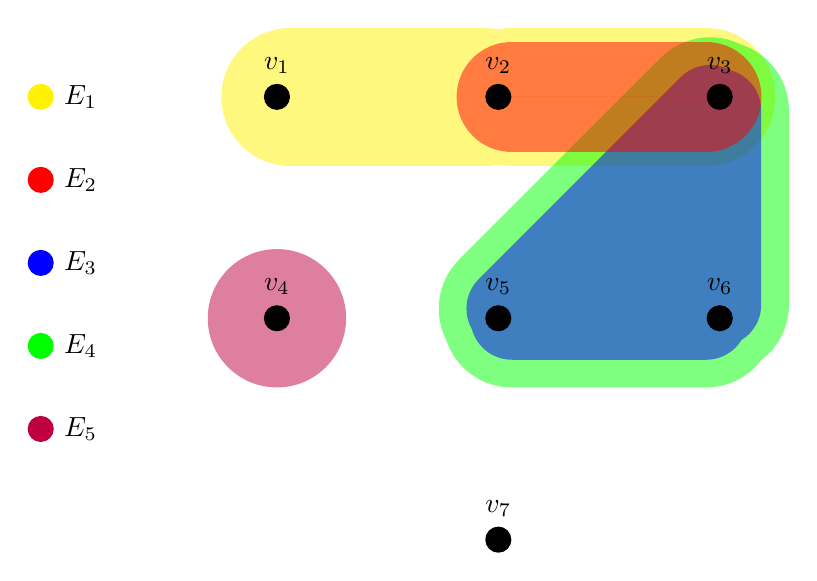
\begin{tikzpicture}
    \tikzstyle{vertex} = [fill,shape=circle,node distance=80pt]
\tikzstyle{edge} = [fill,opacity=.5,fill opacity=.5,line cap=round, line join=round, line width=50pt]
\tikzstyle{edge2} = [fill,opacity=.5,fill opacity=.5,line cap=round, line join=round, line width=30pt]

\tikzstyle{elabel} =  [fill,shape=circle,node distance=30pt]

\pgfdeclarelayer{background}
\pgfsetlayers{background,main}

\node[vertex,label=above:\(v_1\)] (v1) {};
\node[vertex,right of=v1,label=above:\(v_2\)] (v2) {};
\node[vertex,right of=v2,label=above:\(v_3\)] (v3) {};
\node[vertex,below of=v1,label=above:\(v_4\)] (v4) {};
\node[vertex,right of=v4,label=above:\(v_5\)] (v5) {};
\node[vertex,right of=v5,label=above:\(v_6\)] (v6) {};
\node[vertex,below of=v5,label=above:\(v_7\)] (v7) {};

\begin{pgfonlayer}{background}
\draw[edge,color=yellow] (v1) -- (v2) -- (v3);
\begin{scope}[transparency group,opacity=.5]
\draw[edge,opacity=1,color=green] (v3) -- (v5) -- (v6) -- (v3);
\fill[edge,opacity=1,color=green] (v3.center) -- (v5.center) -- (v6.center) -- (v3.center);
\end{scope}

\begin{scope}[transparency group,opacity=.5]
\draw[edge2,opacity=1,color=blue] (v3) -- (v5) -- (v6) -- (v3);
\fill[edge2,opacity=1,color=blue] (v3.center) -- (v5.center) -- (v6.center) -- (v3.center);
\end{scope}
\draw[edge,color=red,line width=40pt] (v2) -- (v3);
\draw[edge,color=purple] (v4) -- (v4);
\end{pgfonlayer}

\node[elabel,color=yellow,label=right:\(E_1\)]  (e1) at (-3,0) {};
\node[elabel,below of=e1,color=red,label=right:\(E_2\)]  (e2) {};
\node[elabel,below of=e2,color=blue,label=right:\(E_3\)]  (e3) {};
\node[elabel,below of=e3,color=green,label=right:\(E_4\)]  (e4) {};
\node[elabel,below of=e4,color=purple,label=right:\(E_5\)]  (e5) {};
\end{tikzpicture}
\end{center}
\end{example}
\begin{definition}
  In a hypergraph $\hgraf=(V,E)$, two vertices $v_i, v_j \in V$ are called 
  \textbf{adjacent} if there is an edge $E_i \in E$ that contains both vertices. 
  Two edges $E_k, E_l$ are called adjacent if there intersection is not empty.
\end{definition}

\begin{definition}
  The \textbf{order of a finite graph \hgraf} is the number of vertices of $\hgraf$ 
  and is denoted by $|\hgraf|$.
\end{definition}
We define now the degree of a vertex in a hypergraph. Note that we don't define 
the indegree and outdegree of vertex as the hypergraphs we consider are 
undirected.
\begin{definition}
The \textbf{degree of a vertex} $v$ in a hypergraph $\hgraf$ is the number of 
times $v$ is contained in an edge.
\end{definition}

\begin{definition}
A \textbf{path} in an hypergraph $\hgraf = (V,E)$ is a sequence $p = (a_0, A_1, a_1, \ldots, A_k, a_k), k \geq 1$ where the
$a_i$'s are pairwise distinct vertices, the $A_i$'s are pairwise distinct
edges and ${a_{i-1}, a_i} \in A_i$ for $1 \leq i \leq k$. The path $p$ is said 
to join $a_0$ and $a_k$. The length of the path is $k$.
\end{definition}

\begin{definition}
A hypergraph is \textbf{connected} if for each vertex there is a path to any 
other vertex.

\end{definition}
\subsubsection{$k$-hypergraphs}
In most applications, the edges of an hypergraph connect a fixed number of 
vertices. This is called a uniform hypergraph:

\begin{definition}
  A \textbf{$k$-uniform hypergraph} with $k \geq 2 \in \N$ if for all $E_i \in E$, 
  the cardinality $|E_i|$ is equal to $k$. The cardinality of multisets is defined in Definition \ref{multiset}.
  The term \textbf{$k$-graph} is often used 
  instead of a $k$-uniform hypergraph. The edges in a $k$-graph are sometimes 
  called $k$-edges.
\end{definition}

Notice that the $2$-hypergraphs are just the undirected graphs we defined in the previous 
section.



\subsubsection{Directed hypergraphs}
An important difference with the previous section is that all hypergraphs we 
have defined are \textbf{undirected}: their is no specific order in which an 
edge connect different vertices. In a graph, directed edges arise naturally as 
some vertex can be the source node and some vertex can be the terminal node, no other nodes
are connected by an edge of a graph. For edges of hypergraphs this concept is not straightforward to generalize: one option is to see 
edges as paths connecting vertices in a specific order,
 another option is to split the vertices connected by an edge in a set of source 
 nodes and a set of terminal nodes. This last notion is 
studied in \cite{gallo}. We will not discuss this topic in detail, all the 
hypergraphs in this master thesis are undirected.


\subsection{Incidence matrix}
A hypergraph can be represented as an incidence matrix by numbering the vertices 
and the edges. The resulting incidence matrix will be a boolean matrix with only 
$1$ and $0$ entries. An alternative way to represent a hypergraph is by using
adjacency tensors. As said in this introduction, these are discussed in chapter 
3.

\begin{definition}\label{incidencematrixhypergraph}
  The \textbf{incidence matrix} of a hypergraph $\hgraf = (V, E)$ with vertices
  $v_1, \ldots, v_n \in V$ and edges $e_1, \ldots, e_m \in E$ is a $n\times m$-matrix $A$ 
  where rows represent the vertices and the columns represent the 
  edges, such that:
  
 $$(A)_{ij} = \begin{cases} 1 &\mbox{if }$v_i \in e_j$   \\ 
0 & \mbox{if } $v_i \not\in e_j$ \end{cases}$$
\end{definition}
\begin{example}
  The corresponding incidence matrix of the hypergraph of Example \ref{vb1hypergraph} 
  is:
  $$\begin{pmatrix}
    1 & 0 & 0 & 0 & 0\\
    1 & 1 & 0 & 0 & 0\\
    1 & 1 & 1 & 1 & 0\\
    0 & 0 & 1 & 1 & 1\\
    0 & 0 & 1 & 1 & 0\\
    0 & 0 & 0 & 0 & 0\\
    0 & 0 & 0 & 0 & 0\\
  \end{pmatrix}.$$
\end{example}







\chapter{Similarity on graphs}

In the previous chapter all the basic terminology and results were introduced, 
now we take an extensive look at the concept of similarity on graphs. Similarity on graphs is a fairly new
concept to compare the nodes of two graphs. The concept arose from the research on algorithms for web searching engines (like \emph{Google}, \emph{Yahoo},\ldots) in the late nineties. 
More specifically, Jon M. Kleinberg 
introduced in his paper `Authoritative Sources in a Hyperlinked Environment' 
\cite{kleinberg} the famous `HITS algorithm' for extracting information from the link structure of websites. The method leads to an iterative algorithm where 
graphs represent the link structure of a collection of websites on a specific topic. Because this paper formed the basis of later research on similarity on graphs, 
the
whole idea and algorithm of Kleinberg is introduced in the first section of this chapter. In 
2004, V.D. Blondel et al. \cite{blondel} generalized the algorithm of 
Kleinberg, introducing the notion of similarity on directed graphs. This similarity is covered in the second section. With this similarity on directed graphs, 
there is a much wider scope of applications than just search algorithms. Next, we extend the notion of similarity on directed graphs: the method
of Blondel only returns the concept of node similarity which is in fact a 
measurement of how similar two nodes of two graphs are to each other.

\section{The HITS algorithm of Kleinberg}
\subsection{History}
Back in the nineties, internet became more and more popular by the public. The popular search 
engines back then where Altavista and Yahoo, but they weren't as advanced as 
search engines today. The main pitfall of the first search engines was that the search results 
were purely based on the number of occurrences of a word in a webpage. This was 
a pitfall for many reasons. The first reason was the growing popularity of the 
internet: as more and more webpages were put online, simply getting the relevant 
pages to a search query in this text-based manner, was a process that could possibly return millions 
of relevant pages. Also \emph{content similarity} was an issue: a website owner 
can easily cheat in a text-based search system by just adding and repeating some 
very popular search words, making his website appear in the results of a large 
number of search queries.
Two possible solutions were simultaneously invented in 1997 and 1998. The first 
one was the
\textit{PageRank}-system developed by Larry Page and Sergey 
Brin (\cite{page}). The PageRank system led to the foundation of the immensely popular Google 
search engine. Meanwhile, also Jon Kleinberg came up with his own solution, the\textit{ HITS algorithm} (hyperlink-induced topic search). At that time,
he was both a professor in the Computer Science Department at the Cornell University and researcher for IBM. The algorithm is 
used inter alia today by the Ask search engine (www.ask.com).
Both these algorithms use the hyperlinks between webpages to rank search 
results. 
Because this master thesis is about similarity and this concept is 
introduced on graphs as a generalization of the HITS algorithm, we don't go to into 
further detail about the PageRank-algorithm. In the following paragraphs, the 
HITS algorithm is extensively explained.

\subsection{Motivation}\label{motivatiehits}
Kleinberg's work originates in the problems that arise with text-based searching the WWW. Text-based searching just counts all the occurrences of a given search query on webpages and returns a set of webpages ordered by decreasing occurency.
When a user 
supplies a search query, we probably face an \textit{abundance problem} with this method: the number of pages that could reasonably be returned as relevant is
far too large for a human user to digest. To provide effective search results 
under these conditions, we need to filter the `authoritative' ones. We face some complications when we
want to filter the `authoritative' webpages in a text-based system. For example, if we search for `\texttt{job offers in Flanders} 
' the most authoritative page and expected first result in a search engine would be \texttt{www.vdab.be}. 
Unfortunately, the query  `\texttt{job offers}' is used in over a 
million pages on the internet and \texttt{www.vdab.be} is not the one using the 
term most often. Therefore, there is no way to favor \texttt{www.vdab.be} in a 
text-based ranking function. This a recurring phenomenon, as another example if 
you search for the query `\texttt{computer brands}', there is no reason at all to be sure that the 
website of Apple or Toshiba even contain this search term.

The HITS algorithm solves these difficulties by analyzing the hyperlink 
structure among webpages. The idea is that hyperlinks encode a sort of human 
judgment and that this judgement is crucial to formulate a notion of authority. 
Specifically, when a page $p$ includes a link to page $q$, it means 
that $p$ gives a \textit{conferred authority} on $q$. Again we face difficulties, because this conferred authority doesn't 
hold for every link. Links are created for a wide variety of reasons, for 
example, a large number of links are created for navigation within a website (e.g. ``Return to homepage'') 
and these have of course nothing to do with a notion of authority. 

The HITS method is based on the relationship between the \textit{authorities} for a topic 
and those pages that link to many related authorities, called \emph{hubs}. Page $p$ 
is called an \textit{authority} for the query ``\texttt{smartphone brand}'' if it 
contains valuable information on the subject. In our example websites of 
smartphone manufacturers such as ``\texttt{www.apple.com}'', 
``\texttt{www.samsung.com}'',... would be good authorities for this search 
query and these are the results a user expect from a search engine. 

A hub is a second category of pages needed to find good authorities. Their role 
is to advertise authoritative pages. Hubs contain useful links toward these 
authorities. In our example, consumer websites with reviews on smartphones, 
websites of smartphone shops,\ldots would be good hubs. In fact, hubs point the 
search process in the `right direction'.

To really grasp the idea, we make an analogy with everyday life. If you tell a 
friend that you think of buying a new smartphone, he might tell you his 
experiences with smartphones and he will probably share some opinions he got from other friends. 
He might suggest you some good models and good brands. Now, you are more inclined to 
buy a smartphone that your friend suggested. Well, this idea is used in the 
HITS-method: your friend served as hub, the brands and models he suggested are good 
authorities.

\subsection{Constructing relevant graphs of webpages}
\begin{algorithm}[t!]

\SetAlgoLined
 \KwData{\\$\sigma$: a query string.\\$\mathcal{E}$: a text-based search engine.\\$t$: natural number (usually initiated to $200$)\\
 $d$: natural number (usually initiated to $50$).}
 \KwResult{A page set $S_\sigma$ satisfying all the properties of our wish list.}
 \blankline
\SetKwFunction{creategraph}{create\_graph}
\SetKwProg{myalg}{begin}{}{end}
\myalg{\creategraph{$\sigma$, $\mathcal{E}$, $t$, $d$}}{
 Let $R_\sigma$ denote the top $t$ results of $\mathcal{E}$ on $\sigma$\;
 Set $S_\sigma := R_\sigma$\;
 \For{each page $p \in R_\sigma$}{
 Let $\Gamma^+(p)$ denote the set of all pages $p$ points to\;
 Let $\Gamma^-(p)$ denote the set of all pages pointing to $p$\;
 Add all pages in $\Gamma^+(p)$ to $S_\sigma$\;
 \eIf{$|\Gamma^-(p)| \leq d$}{
 Add all pages in $\Gamma^-(p)$ to $S_\sigma$\;
 }{
 Add an arbitrary set of $d$ pages from $\Gamma^-(p)$ to $S_\sigma$\;
 }
 }
 \KwRet $S_\sigma$\;}{}
 
 \caption{Algorithm to construct $S_\sigma$.}\label{algoritmegraf}
\end{algorithm}
Any collection of hyperlinked pages can be transformed to a directed graph $\graf = (V, 
\to)$: the nodes correspond to the pages, and if there is a link from page $p$ 
to page $q$, there is an arc $p \to q$. Suppose a search query is performed, 
specified by a query $\sigma$. We wish to determine the authoritative 
pages by an analysis of the link structure. But first we have to construct a 
subgraph of the internet on which our algorithm will operate. We want to make the 
computational effort as efficient as possible, so we restrict the subgraph to 
the set $Q_\sigma$ of all pages where the query $\sigma$ occurs. For this, we could use
any already existing text-based search engine.  But, for our algorithm $Q_\sigma$ 
is possibly much too big: it may contain millions of pages making it impossible 
for any computer to preform the algorithm. Moreover it is, as explained in the motivation in \ref{motivatiehits}, possible that $Q_\sigma$ 
does not contain some of the most important authorities because they never use 
the query string $\sigma$ on their website.

Therefore, we wish to transform the set $Q_\sigma$ to a set $S_\sigma$ of pages following 
this `wish list' of properties:
\begin{enumerate}
  \item $S_\sigma$ is relatively small,
  \item $S_\sigma$ is rich in relevant pages,
  \item$S_\sigma$ contains most of the strongest authorities.
\end{enumerate}
By keeping $S_\sigma$ small, the computational cost of preforming 
non-trivial algorithms can be kept under control. By the property of being rich 
in relevant pages, it will be easier to find good authorities. 

To construct $S_\sigma$, we first construct a \emph{root set} $R_\sigma$ with the $t$ highest-ranked pages for $\sigma$ 
using a text-based search engine (they sort results based on the occurence of 
$\sigma$). Typically, $t$ is set about $200$. $R_\sigma$ complies with properties 1 and 2 
of our wish list, but because $R_\sigma \subset Q_\sigma$, it may fail from satisfying 
property 3. Now we use the root set $R_\sigma$ to create the set $S_\sigma$ satisfying our 
complete wish list. When a strong authority is not in $R_\sigma$, it is very 
likely that at least one of the pages in $R_\sigma$ points to this authority. 
Hence, by using the pages in $R_\sigma$, we can expand it to $S_\sigma$ by looking 
at the links that enter and leave $R_\sigma$. We get algorithm \ref{algoritmegraf}.

Thus, we obtain $S_\sigma$ by expanding
$R_\sigma$ to include any page pointed to by a page in $R_\sigma$. We also add $d$ pages that point
to a page in $R_\sigma$. $d$ is usually initiated to 50. The parameter $d$ is 
crucial to stay in accordance with property 1 of our wish list. Indeed, a 
webpage can be pointed to by several thousands and thousands of other webpages, 
and we don't want to include them all if we want to keep $S_\sigma$ relatively 
small. Some experiments in \cite{kleinberg} showed that this algorithm resulted in a $S_\sigma$ 
with a size in the range of 1000 to 5000 web pages. Property 3 of our wish list is usually met 
because a strong authority need only be reference once in the $t$ pages of the 
root set $R_\sigma$ to be added to $S_\sigma$. 

Denote the resulting graph of the page set $S_\sigma$ by $\graf[S_\sigma]$. Note that $\graf[S_\sigma]$ will 
contain 
a lot of links serving only navigational purposes within a website. As mentioned 
before, these links have nothing to do with the the notion of authority and they must be 
removed from our final graph if we want a good determination of  the authoritative pages by an analysis of
 the link structure.  A very simple heuristic can be used to derive a subgraph 
 of $\graf[S_\sigma]$ leaving out all the navigational links: we make a 
 distinction between \emph{transverse} links and \emph{intrinsic} links. 
 Transverse links are links between different domain names (e.g. a link between \texttt{www.vub.ac.be} and
 \texttt{www.ua.ac.be}) and intrinsic links are links between the same domain 
 name (e.g. a link between \texttt{www.vub.ac.be} and
 \texttt{dwis.vub.ac.be}). Intrinsic links exist to allow navigation within a 
 website and they tell us very little about the authority of the pages they 
 point to. Therefore, we delete all intrinsic links from  $\graf[S_\sigma]$, 
 keeping only the arcs corresponding to transverse links.
 
Our graph still contains some meaningless links in the context of page 
 authority. Suppose a large number of pages from the same domain name have a transverse link to 
 the same page $p$. Most of the time, this means a form of advertisement (by example `Website created by\ldots.' at the bottom of each page). It is useful 
 to only allow $m$ pages ($m$ is usually initiated to 6) from the same domain name to have a transverse link to the same page. 
 If $m$ is exceeded, all the transverse links must be deleted from the graph. Note, 
 however, that not all links to advertisements will be erased because on most 
 web pages, advertisements change on every page which avoids the exceedance of $m$.
 
 Applying the two described heuristics above on $\graf[S_\sigma]$, we get a new 
 graph $\graf'_\sigma$ which is exactly what we need to preform our link analysis.
 
 \subsection{Hubs and Authorities}
 A very simple approach would now be to order the pages in $\graf'_\sigma$ by 
 their indegree. Although this approach can sometimes return good search results, this
 heuristic is often too simple because $S_\sigma$ will probably contain some 
 web pages with a lot of incoming links without being very relevant to the search query $\sigma$ (e.g. advertisements).   
 With these incoming links, those web pages are ranked high in the final search 
 result, which we want to avoid.

 Do we have to return to a text-based approach to avoid irrelevant web pages 
 being on top of the search results? No, the link structure of $\graf'_\sigma$ 
 can tell us a lot more than it may seem at first glance.  Authoritative pages 
 relevant to query $\sigma$ should indeed have a large in-degree, but there should also be a considerable overlap in the sets 
 of pages that point to authoritative pages. This set of pages that point to 
 authoritative pages are called \textit{hubs}. Hubs have links to several 
 authoritative pages and they sort of ``concentrate'' all the authorities on 
 query $\sigma$. Figure \ref{hubauth} shows what this means conceptually.
 \begin{figure}[h!]
  \centering
  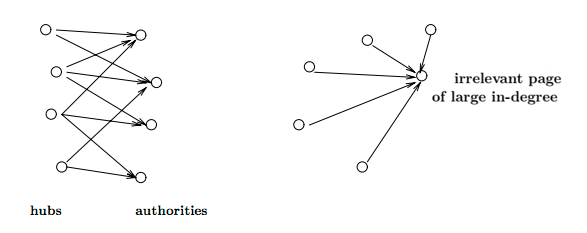
\includegraphics[scale=0.6]{hubauth.png}\caption{The concept of hubs and authorities (Source: \cite{kleinberg})}\label{hubauth}
\end{figure}
 
 So, for each page $j$ we assign two scores, an \textit{authority score} 
 which estimates the value of the content of the page and a \textit{hub 
 score} which estimates the value of the outgoing links to other pages. We get now a\textit{ mutually reinforcing 
 relation}: a good hub is a page pointing to many good authorities, a good 
 authority is a page that is pointed to by many good hubs. This leads us to a 
 \textit{mutually reinforcing relation} resulting in an iterative method to 
 break this circularity.
 
So let $\graf'_\sigma = (V,\to)$ and let $h_j$ and $a_j$ be the hub and authority 
scores of vertex $v_j$ (corresponding with page $j$). These scores must be initialized by some positive start values 
and then updated simultaneously for all vertices. This leads to a \emph{mutually reinforcing relation} 
in which the hub score of $v_j$ is set equal to the sum of the authority scores of all 
vertices pointed to by $v_j$ and in an equal manner the authority score of $v_j$ 
is set equal to the sum of the hub scores of all vertices pointing to $v_j$.

$$\begin{cases} h_j := \sum_{i:(v_j,v_i)\in \to} a_i,\\ 
a_j := \sum_{i:(v_i,v_j)\in \to} h_i.
\end{cases}$$ 

The basic operations in which hubs and authorities reinforce one another are 
depicted in Figure \ref{reinforcing}.
\mathbf{deze tekening wordt nog herwerkt}
\begin{figure}[h!]
  \centering
  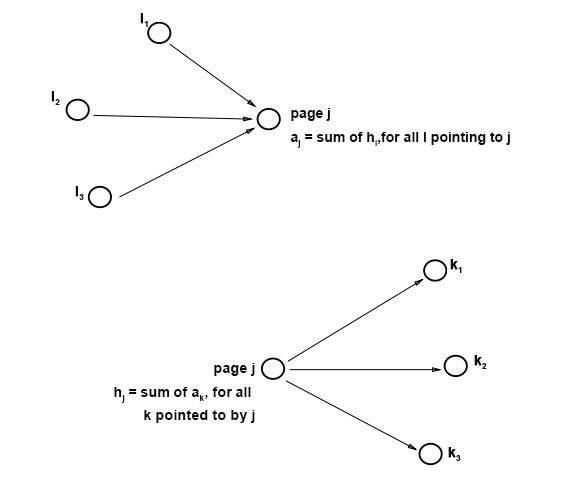
\includegraphics[scale=0.6]{basic.png}\caption{The basic operations in the reinforcing relation between hubs and authorities (Source: \cite{kleinberg})}\label{reinforcing}
\end{figure}

Let $B$ be the adjacency matrix of $\graf'_\sigma$ and denote $\mathbf{a}$ as the authority vector with coordinates $(a_1,a_2,\ldots,a_n)$ (with $n = 
 |\graf'_\sigma|$, the number of pages) and $\mathbf{h}$ as the hub vector. The mutually reinforcing relation can now be rewritten 
as:

$$\begin{pmatrix} 
\textbf{h}\\
\textbf{a}
\end{pmatrix}^{(k+1)} = \begin{pmatrix} 
0 & B\\
B^T & 0
\end{pmatrix} \begin{pmatrix} 
\textbf{h}\\
\textbf{a}
\end{pmatrix}^{(k)},\quad k = 0, 1,\ldots,$$
In compact form, we denote
\begin{eqnarray}\label{compactform}
  \mathbf{x}^{(k+1)} = M\mathbf{x}^{(k)},\quad k = 0, 1,\ldots,
\end{eqnarray}

where 
$$\mathbf{x}^{(k)} = \begin{pmatrix} 
\mathbf{h}\\
\mathbf{a}
\end{pmatrix}^{(k)}, M =  \begin{pmatrix} 
0 & B\\
B^T & 0
\end{pmatrix}$$

After each iteration, we have to normalize $h_j$ and $a_j$. Indeed, we want to get the authority and hub weights for each page
and in order to compare these after each iteration step, they must be normalized because only the relative differences do matter, otherwise the whole procedure would be 
meaningless. Pages with larger $a_j$-scores are viewed as being better authorities, pages with larger $h_j$-scores are better hubs. 

We get the following sequence (with $z^{(0)}$ some positive start value) of normalized vectors: 
\begin{eqnarray}\label{sequencezk}
  \mathbf{z}^{(0)} = \mathbf{x}^{(0)} > 0, \mathbf{z}^{(k+1)} = \frac{M\mathbf{z}^{(k)}}{||M\mathbf{z}^{(k)}||_2}, \quad k = 
  0,1,\ldots,
\end{eqnarray}

How do we decide on $\mathbf{x}^{(0)}$? We will see that any positive vector in $\R^{2n}$ is a good choice, but for the sake of simplicity, we make the natural choice\footnote{$\mathbf{1}$ is a matrix, or vector, whose entries are all equal to 
$1$.} $\mathbf{1} \in \R^{2n}$ . The limit to which the sequence converges 
results in `definitive' hub and authority scores for each page in the graph $\graf'_\sigma$. 

To compute the iterative algorithm, we update the hub and authority scores in an alternating form (by each step we have to normalize the scores). 
Because we will prove that the sequence converges, theoretically we can keep on iterating until a fixed point is approximated. But in most practical settings, 
we choose a fixed number of steps $k$ to reduce the computational cost because we can not know beforehand how
large $k$ has to be to reach the limit. But of course, it is extremely important to know that method converges anyway. Let $\mathbf{x}^{(i)}$ denote vector $\mathbf{x}$ at iteration step $i$ as in Notation \ref{numeriekenotatie}, and we get Algorithm 
\ref{hitsalgorithm}.


\begin{algorithm}[t!]
 \KwData{\\$\graf$: a graph of $n$ linked pages.\\$k$: natural number.}
 \KwResult{A vector $(\mathbf{h}, \mathbf{a})$ containing the hub and authority scores after $k$ steps.}
 \blankline
\SetKwFunction{hits}{hits}
\SetKwProg{myalg}{begin}{}{end}
\myalg{\hits{$\graf$, $k$}}{
 Set $\mathbf{a}^{(0)} = (1,1,\ldots,1) \in \R^n$\;
 Set $\mathbf{h}^{(0)} = (1,1,\ldots,1) \in \R^n$\;
 \For{$i = 1, 2,\ldots,k$}{
 Calculate  $\mathbf{h'}^{(i)} = \left(\sum_{m:(v_1,v_m)\in \to} \mathbf{a}^{(i-1)}_{m}, \sum_{m:(v_2,v_m)\in \to}  \mathbf{a}^{(i-1)}_{m},\ldots, \sum_{m:(v_n,v_m)\in \to}  
 \mathbf{a}^{(i-1)}_{m}\right)$\;
 Normalize  $\mathbf{h'}^{(i)}$ obtaining $\mathbf{h}^{(i)}$\;
 Calculate $\mathbf{a'}^{(i)}=\left(\sum_{m:(v_m,v_1)\in \to} \mathbf{h}^{(i)}_m, \sum_{m:(v_m,v_2)\in \to} \mathbf{h}^{(i)}_m, \ldots, \sum_{m:(v_m,v_n)\in \to} 
 \mathbf{h}^{(i)}_m\right)$\;
 Normalize  $\mathbf{a'}^{(i)}$ obtaining $\mathbf{a}^{(i)}$\;
}

 \KwRet $(\mathbf{h}^{(k)},\mathbf{a}^{(k)} )$\;}{}
 
 \caption{The iterative HITS-algorithm.}\label{hitsalgorithm}
\end{algorithm}

To filter the top $c$ hubs and the top $c$ authorities, you can use the trivial 
Algorithm \ref{filter}. \begin{algorithm}[t!]
 \KwData{\\$\graf$: a graph of $n$ linked pages.\\$k$: natural number.\\$c$: natural number.}
 \KwResult{A vector $((\mathcal{H}_1,\mathcal{H}_2,\ldots, \mathcal{H}_c), (\mathcal{A}_1,\mathcal{A}_2,\ldots, \mathcal{A}_c))$ containing exactly the nodes of the $c$ top hubs and $c$ top authorities.}
 \blankline
\SetKwFunction{filter}{filter}
\SetKwFunction{hits}{hits}

\SetKwProg{myalg}{begin}{}{end}
\myalg{\filter{$\graf$, $k$, $c$}}{
$(\mathbf{h},\mathbf{a}) =$ \hits{$\graf$, $k$}\;
Sort the pages with the $c$ largest values in $\mathbf{h}$, resulting in 
a vector of nodes $(\mathcal{H}_1,\mathcal{H}_2,\ldots, \mathcal{H}_c)$\;
Sort the pages with the $c$ largest values in $\mathbf{a}$, resulting in 
a vector of nodes $(\mathcal{A}_1,\mathcal{A}_2,\ldots, \mathcal{A}_c)$\;

 \KwRet $((\mathcal{H}_1,\mathcal{H}_2,\ldots, \mathcal{H}_c), (\mathcal{A}_1,\mathcal{A}_2,\ldots, \mathcal{A}_c))$\;}{}
 
 \caption{Returning the top $c$ hubs and authorities}\label{filter}
\end{algorithm}

How do we decide on the values of $k$ and $c$? It's immediately clear that $c$ and $k$ must
be proportional: for low $c$ values, a lower 
value for the number of iteration steps $k$ is appropriate and vice versa. 
Experiments in $\cite{kleinberg}$ showed that $k$ set to $20$ is sufficient to 
become stable for finding the $5$ best hubs and authorities, thus for $c = 5$. 

\subsection{Convergence of the algorithm}
We now want to prove that for arbitrarily large values of $k$, the
sequence $Z^{(k)}$ converge to a limit $(\mathbf{h'}, \mathbf{a'})$. Before 
  prove the convergence, note that  adjacency matrices are nonnegative by definition, and thus the matrix $M$ is 
nonnegative too. $M$ is also clearly a symmetric $n' \times n'$-matrix with nonnegative, real entries. We prove that such matrices
have  $n'$ (not necessarily different) real eigenvalues and that we can diagonalize $M$.   This is the first condition of the  
power method iwe introduced in section \ref{powersection}.
If we can also prove the second condition (having a unique dominant eigenvalue), 
convergence is immediately shown by the power method.

However, there is a problem here: we can not prove that nonnegative symmetric matrices have a unique dominant 
eigenvalue (a unique dominant eigenvalue means the largest eigenvalue with multiplicity 1), simply because this is not true in general.\footnote{The matrix $\begin{pmatrix} 
1 & 0\\
0 & 1
\end{pmatrix}$ is a simple counterexample of a symmetric, nonnegative, real matrix that has no unique dominant eigenvalue.} 
In the original paper of Kleinberg \cite{kleinberg} he solves this issue by 
simply imposing that the matrix $M$ has a unique dominant eigenvalue and he doesn't pay any further attention to this problem.  
He presents it as `a small, technical assumption for the sake of simplicity'.

Is this justified in practice? Actually it is, because you can prove with probability theory that a random 
matrix $C_n$,  with a probability tending to 1, has no repeated eigenvalues as the size of the matrix goes to infinity (See for example Thereom 2.2.3 in \cite{random}).  You can also defend this differently: the only reason why we can't use the 
Perron-Frobenius theorem (see \ref{frobtheorem}) here, is because $M$ will have 
zero entries (not all pages in $S_\sigma$ will be linked to each other, the graph $\graf'_\sigma$ is not strongly connected in general). But,
it is intuitively clear that by adding 1 to each entry of $M$, the final results 
of the algorithm (a sorted vector with the best hubs and authorities) will not 
be changed at all, because pages with larger indegrees and outdegrees will continue to get better hub and authority scores (note, however, that the relative hub and authority scores can fluctuate a bit and the algorithm will converge slower because of the lack of zero 
entries). So, by adding 1 to each entry of $M$, the matrix becomes a positive, real matrix 
and we know from the Perron-Frobenius that these matrices have a unique dominant 
eigenvalue. So yes, the `small, technical assumption' in the paper of Kleinberg 
is justified.

Now that this problem is solved, we present the relevant theorems below. We also 
impose on the matrix $M$ that it has a unique dominant eigenvalue with the preceding explanations in mind. 
Remember that we will generalize the idea of the HITS algorithm to introduce 
similarity on graphs. Therefore, we will reconsider the 
convergence of the (generalized) algorithm again in the following section, and 
there we prove that there exists also a limit even when the matrix $M$ has no unique 
dominant eigenvalue. The reason why we don't present this result immediately, is 
because we want to present the results as authentic possible and we want to show 
the evolution of the ideas in the successive papers.

\begin{theorem}
  If $A$ is a symmetric, real $n\times n$-matrix, then it has $n$ (not necessarily different) real eigenvalues corresponding
  to real eigenvectors.
  \end{theorem}
  \begin{proof}
    First, threat $A$ as complex matrix.
    The characteristic polynomial $\det(A-\lambda I)$ has $n$ roots in $\C$ and 
    each root is an eigenvalue for $A$. Let $\lambda \in \C$ be any eigenvalue 
    and $\mathbf{v} \in \C^n$ be a corresponding eigenvector for $A$. We have:
    $$A\mathbf{v} = \lambda\mathbf{v}.$$ As $A = A^t$, we also get:
    $$\mathbf{v}^tA = \lambda \mathbf{v}^t.$$
    Taking the complex conjugate of both sides we get ($A$ is a real matrix):
    $$\bar{\mathbf{v}}^tA = \bar{\lambda}\bar{\mathbf{v}}^t$$
    We get:
    $$\bar{\mathbf{v}}^tA\mathbf{v} = (\bar{\mathbf{v}}^tA)\mathbf{v} = (\bar{\lambda}\bar{\mathbf{v}}^t)\mathbf{v} 
    = \bar{\lambda}\bar{\mathbf{v}}^t\mathbf{v}.$$
    We also have:
    $$\bar{\mathbf{v}}^tA\mathbf{v} = \bar{\mathbf{v}}^t(A\mathbf{v}) = 
    \lambda\bar{\mathbf{v}}^t\mathbf{v}.$$
    Hence:
    $$\bar{\lambda}\bar{\mathbf{v}}^t\mathbf{v} = \lambda\bar{\mathbf{v}}^t\mathbf{v}.$$
    We conclude that $\lambda = \bar{\lambda}$ for $\mathbf{v} \not = 0$. 
    We proved that every eigenvalue of $A$ is real. If $\lambda$ is an 
    eigenvalue of $A$, then the matrix $(A - \lambda I)$ is not invertible so a 
    vector $\mathbf{s} \in \R^n$ exists with $$(A - \lambda I)\mathbf{s} = 0,$$ 
    proving that also the corresponding eigenvector is real.
    
  \end{proof}
\begin{theorem}\label{diagonaal}\textbf{(Symmetric Schur Decomposition)}
  Let $A$ be a real symmetric matrix, then there exist an orthogonal 
  matrix $P$ such that:
  \begin{enumerate}
    \item[(i)] $P^{-1}AP = D$, a diagonal matrix,
    \item[(ii)] The diagonal entries of $D$ are the eigenvalues of $A$,
    \item[(iii)] The column vectors of $P$ are the eigenvectors of the 
    eigenvalues of $A$.
  \end{enumerate}
\end{theorem}
 \begin{proof}
By induction on the order of the matrix. For $n=1$ the theorem is trivial. Let $A$ 
be a symmetric $n\times n$-matrix. $A$ has at least one eigenvalue $\lambda_1$ by the 
previous theorem. Let $\mathbf{x_1}$ be a corresponding eigenvalue with $\|\mathbf{x}_1\|=1$ 
and $A\mathbf{x}_1=\lambda_1\mathbf{x}_1$. By the Gram-Schmidt procedure, we construct an 
orthonormal basis $V_1 = \{\mathbf{x}_1, \mathbf{v}_2,\ldots,\mathbf{v}_n\}$ of 
$\R^n$.
Let:
$$S_1= [\mathbf{x}_1,\mathbf{v}_2,\ldots,\mathbf{v}_n],$$
since $S_1$ is orthonormal, we get $S^t_1 = S^{-1}$. Consider the matrix:
$S_1^{-1}AS_1$. We have:
$$(S_1^{-1}AS_1)^t = (S_1^{t}AS_1)^t = S_1^t A^t S_1 = S^{-1}_1AS_1$$
Thus $S_1^{-1}AS_1$ is a symmetric matrix. Since $S_1\mathbf{e}_1 = \mathbf{x}_1$, we get:
\begin{eqnarray*}
 S_1^{-1}AS_1\mathbf{e}_1 &=& (S_1^{-1} A)(\mathbf{x}_1)\\
 &=& S_1^{-1}(\lambda_1\mathbf{x}_1)\\
 &=& \lambda_1(S_1^{-1}\mathbf{x}_1)\\
 &=& \lambda_1 \mathbf{e}_1
\end{eqnarray*}
So we get:
$$S_1^{-1}AS_1=\left(
\begin{array}{c|c}
\lambda_1 & \mathbf{0} \\ \hline
\mathbf{0}^t & A_1
\end{array}\right),$$
with $\mathbf{0}$ a vector of zero entries of size $n-1$ and $A_1$ an $(n-1)\times(n-1)$ symmetric matrix. 
We know by induction that there exist a $(n-1)\times(n-1)$ orthogonal matrix $S_2$ such that 
$S_2^{-1}A_1S_2 = D'$ with $D'$ an  $(n-1)\times(n-1)$ diagonal matrix. Let:
$$S'_2=\left(
\begin{array}{c|c}
1 & \mathbf{0} \\ \hline
\mathbf{0}^t & S_2
\end{array}\right),$$
and also $S'_2$ is an orthogonal matrix, we get:
\begin{eqnarray*}
 \left(S'_2\right)^{-1}S_1^{-1}A S_1 S'_2 &=& \left(
\begin{array}{c|c}
1 & \mathbf{0} \\ \hline
\mathbf{0}^t & S^t_2
\end{array}\right) \left(S_1^{-1}A S_1\right) \left(
\begin{array}{c|c}
1 & \mathbf{0} \\ \hline
\mathbf{0}^t & S_2
\end{array}\right) \\
&=& \left(
\begin{array}{c|c}
1 & \mathbf{0} \\ \hline
\mathbf{0}^t & S^t_2
\end{array}\right) 
\left(
\begin{array}{c|c}
\lambda_1 & \mathbf{0} \\ \hline
\mathbf{0}^t & A_1
\end{array}\right) 
 \left(
\begin{array}{c|c}
1 & \mathbf{0} \\ \hline
\mathbf{0}^t & S_2
\end{array}\right) \\
&=& 
 \left(
\begin{array}{c|c}
\lambda_1 & \mathbf{0} \\ \hline
\mathbf{0}^t & S^t_2A_1S_2
\end{array}\right) \\
&=&
 \left(
\begin{array}{c|c}
\lambda_1 & \mathbf{0} \\ \hline
\mathbf{0}^t & D'\end{array}\right) 
\end{eqnarray*}
Thus, if we put
\begin{eqnarray*}
P &=& S_1S'_2\\
D &=& \left(
\begin{array}{c|c}
\lambda_1 & \mathbf{0} \\ \hline
\mathbf{0}^t & D'\end{array}\right),
\end{eqnarray*}
we have proved (1). From the definition of diagonalizable matrices and Theorem \ref{eigenbasis} 
(ii) and (iii) immediately follow.
\end{proof}
 \begin{theorem}
   Giving a graph $\graf$ with $n$ linked pages, the sequence as defined in the previous paragraph: 
   $$\mathbf{z}^{(0)} = \mathbf{1} \in \R^{n}, \mathbf{z}^{(k+1)} = \frac{M\mathbf{z}^{(k)}}{||M\mathbf{z}^{(k)}||_2}, \quad k = 
  0,1,\ldots,$$
  converges when $M$ has a unique dominant eigenvalue.
 \end{theorem}
\begin{proof}
  Since 1) $M$ is diagonalizable as symmetric matrix by Theorem \ref{diagonaal}  
  and 2) $M$ has a unique dominant eigenvalue, it follows from the power method that
  the sequence will converge to a corresponding dominating eigenvector $(\mathbf{h'}, \mathbf{a'})$. This eigenvector contains the hub and authority scores.
  \end{proof}


We conclude with a nice corollary.

\begin{corollary}
The second power of the matrix $M$ has the form:
$$M^2 = \begin{pmatrix} 
BB^T & 0\\
0 & B^TB
\end{pmatrix},$$
and the normalized hub and authority scores are given by the 
dominant eigenvectors of $BB^T$ and $B^TB$.\end{corollary}
 
 \begin{proof}
     By the compact form given in equation \ref{compactform}, we see that $\mathbf{h_k} \leftarrow (BB^T)^{k-1}B\mathbf{a_0}$ 
     and $\mathbf{a_k} \leftarrow (B^TB)^{k}\mathbf{a_0}$. Let $\mathbf{a_0}$ be $\mathbf{1} \in \R^n$. From the previous theorem we 
     also know that:
     $$\lim_{k\to\infty}\mathbf{h_k} = \mathbf{h} \quad \text{and} \quad \lim_{k\to\infty}\mathbf{a_k} = \mathbf{a},$$
     and also from the previous proof we know that $(\mathbf{h}, \mathbf{a})$ is 
     the dominant eigenvector of $M$. It follows immediately that also 
     $\mathbf{h}$ is the dominant eigenvector of $BB^T$ and $\mathbf{a}$ is the dominant eigenvector of 
     $B^TB$.
 \end{proof}
 \subsection{Examples}
 \subsubsection{Searching for math professors at the VUB}
\begin{example}
  We conclude this section with a fictitious example of the HITS-algorithm. Suppose you 
  are looking for \texttt{math professors vub} with a text-based search engine 
  and you get the following results:
  \begin{itemize}
    \item The website of the mathematics department of the VUB,
       \item The website of the faculty of science of the VUB,
    \item The websites of 4 math professors,
    \item The website of 10 PhD students at the the mathematics department of the VUB.
  \end{itemize}
Lets take a look at the link structure of these web pages (remember that it is a fictitious example):
  \begin{itemize}
    \item The website of the mathematics department at the VUB links to the websites of all the 4 professors, 
    the 10 PhD students and the faculty of science,
   
      \item The website of the faculty of science of the VUB links to the websites 
    of all the 4 math professors and the mathematics department,
    
 \item The websites of the 4 math professors link to the website of the 
    Mathematics department and the faculty of science,

    \item The websites of the 10 PhD students at the the VUB link to the the 
    website of their promotor. 1 professor has 4 PhD students, the other 3 professors 
    have 2 PhD students.
      \end{itemize}
We can now construct the graph $\graf_\sigma$ (of course this graph is not completely made according to Algorithm \ref{algoritmegraf}) and we have the following adjacency matrix of 
$\graf_\sigma$:
\setcounter{MaxMatrixCols}{20}
\begin{itemize}
  \item \textbf{Row 1}: website of the mathematics department,
    \item \textbf{Row 2}: website of the faculty of science,
    \item  \textbf{Row 3}: website of the professor with the 4 PhD students,
    \item  \textbf{Row 4, 5, 6}: websites of the professors with the 2 PhD students,
    \item  \textbf{Row 7, 8, 9, 10}: websites of the 4 PhD students of the professor on row 3,
    \item  \textbf{Row 11, 12}: websites of the 2 PhD students of the professor on row 4,
    \item  \textbf{Row 12, 14}: websites of the 2 PhD students of the professor on row 5,
    \item  \textbf{Row 14, 16}: websites of the 2 PhD students of the professor on row 6,


\end{itemize}
Leads to:
$$
 B= \begin{pmatrix} 
0 & 1 & 1 & 1 & 1 & 1 & 1 & 1 & 1 & 1 & 1  & 1 & 1 & 1 & 1 & 1\\
1 & 0 & 1 & 1 & 1 & 1 & 0 & 0 & 0 & 0 & 0 & 0 & 0 & 0 & 0 & 0 \\
1 & 1 & 0 & 0 & 0 & 0 & 0 & 0 & 0 & 0 & 0 & 0 & 0 & 0 & 0 & 0 \\
1 & 1 & 0 & 0 & 0 & 0 & 0 & 0 & 0 & 0 & 0 & 0 & 0 & 0 & 0 & 0 \\
1 & 1 & 0 & 0 & 0 & 0 & 0 & 0 & 0 & 0 & 0 & 0 & 0 & 0 & 0 & 0 \\
1 & 1 & 0 & 0 & 0 & 0 & 0 & 0 & 0 & 0 & 0 & 0 & 0 & 0 & 0 & 0 \\
0 & 0 & 1 & 0 & 0 & 0 & 0 & 0 & 0 & 0 & 0 & 0 & 0 & 0 & 0 & 0 \\
0 & 0 & 1 & 0 & 0 & 0 & 0 & 0 & 0 & 0 & 0 & 0 & 0 & 0 & 0 & 0 \\
0 & 0 & 1 & 0 & 0 & 0 & 0 & 0 & 0 & 0 & 0 & 0 & 0 & 0 & 0 & 0 \\
0 & 0 & 1 & 0 & 0 & 0 & 0 & 0 & 0 & 0 & 0 & 0 & 0 & 0 & 0 & 0 \\
0 & 0 & 0 & 1 & 0 & 0 & 0 & 0 & 0 & 0 & 0 & 0 & 0 & 0 & 0 & 0 \\
0 & 0 & 0 & 1 & 0 & 0 & 0 & 0 & 0 & 0 & 0 & 0 & 0 & 0 & 0 & 0 \\
0 & 0 & 0 & 0 & 1 & 0 & 0 & 0 & 0 & 0 & 0 & 0 & 0 & 0 & 0 & 0 \\
0 & 0 & 0 & 0 & 1 & 0 & 0 & 0 & 0 & 0 & 0 & 0 & 0 & 0 & 0 & 0 \\
0 & 0 & 0 & 0 & 0 & 1 & 0 & 0 & 0 & 0 & 0 & 0 & 0 & 0 & 0 & 0 \\
0 & 0 & 0 & 0 & 0 & 1 & 0 & 0 & 0 & 0 & 0 & 0 & 0 & 0 & 0 & 0 \\
\end{pmatrix},$$

Intuitively, we expect that the professor with his 4 PhD 
student will have the largest authority score, immediately followed by the other 3 professors.
The website of the mathematics department is clearly the best hub in this example and should get the largest hub score.
Also the website of the faculty of science should get a high hub score.

We now apply the HITS-method by
calculating the dominant eigenvector of $BB^T$ (this returns the hub scores) 
and the dominant eigenvector of $B^TB$ (this returns the authority scores) with 
the power method (see \ref{powersection}). We get:


$$ \mathbf{a} = \begin{pmatrix}
0.1979\\
0.3162\\
\mathbf{0.3688}\\
0.3231\\
0.3231\\
0.3231\\
0.2029\\
0.2029\\
0.2029\\
0.2029\\
0.2029\\
0.2029\\
0.2029\\
0.2029\\
0.2029\\
0.2029\\
\end{pmatrix} \quad \text{and} \quad
\mathbf{h} = \begin{pmatrix}
\mathbf{0.8645}\\
0.3605\\
0.1207\\
0.1207\\
0.1207\\
0.1207\\
0.0866\\
0.0866\\
0.0866\\
0.0866\\
0.0758\\
0.0758\\
0.0758\\
0.0758\\
0.0758\\
0.0758\\
\end{pmatrix}
$$

We see that the websites of the 4 math professors are indeed the best authorities for the search 
query \texttt{math professors vub} and that the website of the mathematics department is an 
extremely good hub (this is very logic because it links to all the other relevant 
websites). The professor with his 4 PhD students would be ranked first in the 
search results (he has the highest authority score), the other professors would 
appear just underneath him. Obviously, a hub score of 0.8645 is so high that it would be quite exceptional in 
a graph containing a lot more websites (it's very unlikely that you find a website containing links to all the other pages/nodes in the graph). Nevertheless, we conclude that the HITS-algorithm returns the 
results we wanted intuitively.

\end{example}
 \subsubsection{Predictors in the Eurovision Song Contest 2009-2014}
 The Eurovision Song Contest is an annual competition between countries whose 
 public broadcaster is part of the EBU-network. The contest is the biggest music 
 competition in the world, reaching about 200 million anually.
  
 The contest consists of three shows: 2 semi-finals and 1 grand final. From each 
 semi-final, 10 countries proceed the the grand final. Italy, Germany, Spain, United Kingdom and France are 
 always qualified for the grand final because they are the main funders of the event. 
 Also the winner of last year participates automatically in the final. Each country, also those 
 who dropped out during the semi-finals, gives points during the voting of the grand final. 
The voting during the grand final takes place after all the countries have performed their song. 
Each country is called and and awards 12 points to their 
favorite song, 10 points to their second favorite, and then points from 8 down 
to 1 to eight other songs. Countries can not vote for themselves. 

The voting 
system is in fact a positional voting system that is very similar to the Borda count 
method (see \cite{saari} for a scientific explanation of Borda count): the list 
of points of a country represents the ranking of the 10 best countries in the voting of that country. 
So the points are values on an ordinal scale.

The complete voting procedure during the Eurovision Song Contest can be seen as 
a directed graph: all the participating countries are the nodes and the edges 
represent the points between the countries (when country $a$ assigns 3 points to country $b$, then there are 3 edges from $a$ to 
$b$).

Let $A$ be the adjacency matrix of the voting during a song contest ($A$ will in fact be just a points table). If we 
take $A$ as input for the HITS-algorithm, we expect that the country with the 
highest authority score will be the winner of the competition. Actually we 
expect a lot more: when we order the countries based on their authority score, 
we expect that this ordering will be practically equal to the final ranking of the contest. 
This is based on the simple fact that Borda count just sums up points, and we 
only expect very small differences when the difference in points is low between 
two countries. This small differences are then be caused by the algorithm: remember 
that the HITS-algorithm does not simply give a high authority score to nodes 
with a large indegree, but also takes the hub scores into account, but we will 
see that the hub scores will be low so their influence will indeed be limited.

But what is very interesting now, is the role that the hub scores are playing. 
In fact these scores can be seen as a kind of `predictive value' of a country: a 
country with a high hub score will have assigned points in such way that it is 
seen as a reliable source, meaning that the points of that country will match 
well with the final result of the contest. 

Let's take the Eurovision Song Contest 2014 as an example. 

The final results of the contest where (the complete result table can be found in Appendix 
B):
\begin{enumerate}
  \itemsep0em
\item Austria (290 points)
\item The Netherlands (238 points)
\item Sweden (218 points)
\item Armenia (174 points)
\item Hungary (143 points)
\item Ukraine (113 points)
\item Russia (89 points)
\item Norway (88 points)
\item Denmark (74 points)
\item Spain (74 points)
\item Finland (72 points)
\item Romania (72 points)
\item Switzerland (64 points)
\item Poland (62 points)
\item Iceland (58 points)
\item Belarus (43 points)
\item United Kingdom (40 points)
\item Germany (39 points)
\item Montenegro (37 points)
\item Greece (35 points)
\item Italy (33 points)
\item Azerbaijan (33 points)
\item Malta (32 points)
\item San Marino (14 points)
\item Slovenia (9 points)
\item France (2 points)
\end{enumerate}
Now we calculate the hub and authority scores, based on the full scoreboard and 
the results are presented in Table \ref{t2014}.
\begin{table}[h!]
  \centering

\begin{tabular}{l | r}
\textbf{Participant}     & \textbf{Authority Score}\\\hline 
Austria         & 0.285110029     \\
The Netherlands & 0.235720093     \\
Sweden          & 0.212949392     \\
Armenia         & 0.156091783     \\
Hungary         & 0.124453384     \\
Ukraine         & 0.095410297     \\
Norway          & 0.086504385     \\
Denmark         & 0.074474911     \\
Finland & 0.070675128     \\
Spain           & 0.068432379     \\
Russia          & 0.065352465     \\
Romania         & 0.062560768     \\
Switzerland     & 0.055868228     \\
Iceland         & 0.053973263     \\
Poland          & 0.052246035     \\
United Kingdom  & 0.037978889     \\
Germany         & 0.029958317     \\
Belarus         & 0.027945852     \\
Malta           & 0.026911408     \\
Italy           & 0.023817428     \\
Montenegro      & 0.023425296     \\
Azerbaijan      & 0.022613716     \\
Greece          & 0.021816155     \\
San Marino      & 0.009315756     \\
Slovenia        & 0.005843162     \\
France  & 0.002167387     \\
Albania         & 0               \\
Belgium         & 0               \\
Estonia         & 0               \\
FYR Macedonia   & 0               \\
Georgia         & 0               \\
Ireland         & 0               \\
Israel          & 0               \\
Latvia          & 0               \\
Lithuania       & 0               \\
Moldova         & 0               \\
Portugal        & 0              
\end{tabular}
$\;\;\;$
\begin{tabular}{l|r}
\textbf{Participant}     & \textbf{Hub Score}   \\\hline 
Portugal        & 0.173610946 \\
Finland         & 0.172574335 \\
Belgium         & 0.169584694 \\
Latvia          & 0.166295198 \\
Spain           & 0.165764986 \\
Hungary         & 0.165699760  \\
Iceland         & 0.165062483 \\
Estonia         & 0.162056401 \\
Denmark         & 0.160549539 \\
Lithuania       & 0.159920120  \\
Greece          & 0.159278464 \\
Norway          & 0.156676045 \\
Slovenia        & 0.156533823 \\
Sweden          & 0.155725338 \\
Romania         & 0.155212094 \\
France          & 0.153993935 \\
Switzerland     & 0.153864143 \\
Israel          & 0.153059334 \\
Ireland         & 0.147584917 \\
The Netherlands & 0.145211066 \\
United Kingdom  & 0.144342619 \\
Austria         & 0.137956312 \\
Germany         & 0.136869443 \\
Ukraine         & 0.135769452 \\
Italy           & 0.121638547 \\
Malta           & 0.119063784 \\
Georgia         & 0.117423087 \\
Moldova         & 0.115874904 \\
Poland          & 0.112296570  \\
FYR Macedonia   & 0.107531180  \\
Russia          & 0.102149330  \\
San Marino      & 0.098204303 \\
Montenegro      & 0.097193444 \\
Albania         & 0.091897617 \\
Belarus         & 0.089227164 \\
Azerbaijan      & 0.068005452 \\
Armenia         & 0.050899422
\end{tabular}

\caption{The authority and hub scores of the countries during the Final of the Eurovision Song Contest 2014}
\end{table}\label{t2014}

Notice that ordering the countries by their authority scores indeed returns the final ranking of the contest. The countries who have an
authority score equal to 0 are the countries that didn't make it to the final and couldn't therefore 
receive any points. When looking at the hub scores, it appears that Portugal `predicted' the 
final ranking the best. When we look at the points awarded by Portugal during 
the final, this is indeed true:
\begin{itemize}
  \itemsep0em

  \item \textbf{12 points}: Austria
\item \textbf{10 points}: The Netherlands
\item \textbf{8 points}: Sweden
\item \textbf{7 points}: Switzerland	
\item \textbf{6 points}: Hungary
\item \textbf{5 points}: Denmark
\item \textbf{4 points}: Armenia	
\item \textbf{3 points}: Norway
\item \textbf{2 points}: Russia
\item \textbf{1 point}: Romania
\end{itemize}
No less than 7 countries in the points of Portugal have achieved the final top 
10, the top 3 results of Portugal are even equal to the final top 3! Russia, Romania and
Switzerland are the 3 countries where Portugal awarded points to but didn't achieve the 
top 10, but still they are placed 11$^\text{\th}$, 12$^\text{\th}$ and 
13$^\text{\th}$ in the final ranking. So it is absolutely not surprising that Portugal is the country 
with the highest hub score. 

Note that countries who scored very well during 
the final, usually have a moderate hub score: this is due to the fact that 
countries can not vote for themselves. The average hub score is, in general, also 
lower than the average authority score, this is because countries can award 
points to only 10 countries, but (qualified) countries can receive points from 
every country, except themselves. The `predictive value' of a country is 
therefore limited to only 10 countries, while the voting produces a complete final ranking of 26 
countries.

Of course, it's tempting to research the predictive value of countries during a 
couple of years. We opted for the period 2009-2014 because during the last five 
years the voting procedure remained unchanged: the points awarded by each country are based on 50$\%$ televoting and
$50\%$ jury vote. So we take the average of the hub scores of the last five 
years of each country. We only put one condition on these countries: they should 
have participated at 4 out of 5 times, more than 1 absence would possibly make the average misleading.
The result is presented in Table \ref{thub}. The complete results of each year can be found in Appendix B. 

We see that Hungary, Cyprus and Belgium are the best predictors during the last 
five years. The bottom is also not very surprising: in 2010, 2012 and 2013 Albania did not 
receive enough televotes so the jury decided their points (see \cite{eurovision} for more information), making their judging process vary from one year to another.
Azerbaijan and Armenia scored very high in the last five years, (e.g. Azerbaijan reached the top 5
every year except 2014, won in 2011 and became second in 2013) 
but due to their dispute about the Nagorno-Karabakh region, they never exchanged a 
single
point during the last five years. Also cultural differences are probably an 
explanation: Georgia, Azerbaijan and Armenia are located in the Caucasus, a remote corner of Europe, with 
many Asian influences (the region is sometimes refered to as Eurasia). 

\begin{table}[h!]
\begin{tabular}{|l|r|r|r|r|r|r|r|r|}
\hline
\textbf{Participant}                                       & \textbf{2014} & \textbf{2013} & \textbf{2012} & \textbf{2011} & \textbf{2010} & \textbf{2009} & \textbf{Average}  \\ \hline
Hungary                                                    & 0.165700      & 0.150320      & 0.151291      & 0.130650      & -             & 0.158260      & \textbf{0.151244} \\ \hline
Cyprus                                                     & -             & 0.161413      & 0.140385      & 0.145691      & 0.144175      & 0.146567      & \textbf{0.147646} \\ \hline
Belgium                                                    & 0.169585      & 0.159189      & 0.153462      & 0.118487      & 0.147362      & 0.122234      & \textbf{0.145053} \\ \hline
Lithuania                                                  & 0.159920      & 0.141552      & 0.144121      & 0.127425      & 0.144634      & 0.152601      & \textbf{0.145042} \\ \hline
\begin{tabular}[c]{@{}l@{}}The \\ Netherlands\end{tabular} & 0.145211      & 0.133926      & 0.147638      & 0.137637      & 0.139085      & 0.163395      & \textbf{0.144482} \\ \hline
Israel                                                     & 0.153059      & 0.157744      & 0.139948      & 0.131677      & 0.118970      & 0.157031      & \textbf{0.143072} \\ \hline
Spain                                                      & 0.165765      & 0.153609      & 0.133174      & 0.114255      & 0.162626      & 0.122739      & \textbf{0.142028} \\ \hline
Latvia                                                     & 0.166295      & 0.134627      & 0.138436      & 0.121329      & 0.142837      & 0.143788      & \textbf{0.141219} \\ \hline
Estonia                                                    & 0.162056      & 0.141096      & 0.131495      & 0.143254      & 0.136098      & 0.131401      & \textbf{0.140900} \\ \hline
Slovenia                                                   & 0.156534      & 0.141375      & 0.148665      & 0.118682      & 0.137277      & 0.133178      & \textbf{0.139285} \\ \hline
Malta                                                      & 0.119064      & 0.146482      & 0.122804      & 0.162192      & 0.138073      & 0.139682      & \textbf{0.138049} \\ \hline
Iceland                                                    & 0.165062      & 0.149906      & 0.129060      & 0.130358      & 0.137492      & 0.113493      & \textbf{0.137562} \\ \hline
Denmark                                                    & 0.160550      & 0.112496      & 0.139704      & 0.104782      & 0.144174      & 0.156365      & \textbf{0.136345} \\ \hline
Greece                                                     & 0.159278      & 0.144943      & 0.124054      & 0.145912      & 0.095629      & 0.148054      & \textbf{0.136312} \\ \hline
Austria                                                    & 0.137956      & 0.127058      & 0.153796      & 0.129429      & -             & 0.132217      & \textbf{0.136091} \\ \hline
Croatia                                                    & -             & 0.169310      & 0.132023      & 0.129980      & 0.114014      & 0.134540      & \textbf{0.135974} \\ \hline
France                                                     & 0.153994      & 0.135187      & 0.151435      & 0.137268      & 0.118194      & 0.109034      & \textbf{0.134185} \\ \hline
Russia                                                     & 0.102149      & 0.130277      & 0.129907      & 0.143360      & 0.141861      & 0.152992      & \textbf{0.133424} \\ \hline
Sweden                                                     & 0.155725      & 0.122816      & 0.099063      & 0.106864      & 0.153858      & 0.160329      & \textbf{0.133109} \\ \hline
Ireland                                                    & 0.147585      & 0.137790      & 0.132864      & 0.103704      & 0.147411      & 0.128126      & \textbf{0.132913} \\ \hline
Romania                                                    & 0.155212      & 0.141742      & 0.119829      & 0.131675      & 0.128084      & 0.119466      & \textbf{0.132668} \\ \hline
Germany                                                    & 0.136869      & 0.126650      & 0.157167      & 0.103942      & 0.115909      & 0.155134      & \textbf{0.132612} \\ \hline
Finland                                                    & 0.172574      & 0.108008      & 0.141472      & 0.101891      & 0.133330      & 0.132773      & \textbf{0.131675} \\ \hline
Bulgaria                                                   & -             & 0.136342      & 0.150772      & 0.110776      & 0.136208      & 0.122794      & \textbf{0.131378} \\ \hline
Norway                                                     & 0.156676      & 0.098933      & 0.154850      & 0.099012      & 0.155455      & 0.107546      & \textbf{0.128745} \\ \hline
\begin{tabular}[c]{@{}l@{}}United \\ Kingdom\end{tabular}  & 0.144343      & 0.143615      & 0.121922      & 0.096917      & 0.136172      & 0.133630      & \textbf{0.128594} \\ \hline
Portugal                                                   & 0.173611      & -             & 0.116836      & 0.130723      & 0.107674      & 0.105899      & \textbf{0.126949} \\ \hline
Serbia                                                     & -             & 0.165969      & 0.113907      & 0.095025      & 0.132455      & 0.123080      & \textbf{0.126087} \\ \hline
Ukraine                                                    & 0.135769      & 0.106438      & 0.123998      & 0.120992      & 0.139278      & 0.142826      & \textbf{0.125295} \\ \hline
\begin{tabular}[c]{@{}l@{}}FYR \\Macedonia\end{tabular}                                           & 0.107531      & 0.138521      & 0.132612      & 0.116197      & 0.127626      & 0.124228      & \textbf{0.124453} \\ \hline
Belarus                                                    & 0.089227      & 0.143351      & 0.120914      & 0.138934      & 0.104108      & 0.149588      & \textbf{0.124354} \\ \hline
Moldova                                                    & 0.115875      & 0.139519      & 0.119439      & 0.126125      & 0.119696      & 0.119161      & \textbf{0.123302} \\ \hline
Switzerland                                                & 0.153864      & 0.117585      & 0.125128      & 0.092621      & 0.127077      & 0.117733      & \textbf{0.122335} \\ \hline
Georgia                                                    & 0.117423      & 0.147386      & 0.123067      & 0.132744      & 0.086281      & -             & \textbf{0.121380} \\ \hline
Albania                                                    & 0.091898      & 0.102282      & 0.098185      & 0.142108      & 0.140538      & 0.141493      & \textbf{0.119417} \\ \hline
Azerbaijan                                                 & 0.068005      & 0.109553      & 0.113396      & 0.119173      & 0.120818      & 0.109357      & \textbf{0.106717} \\ \hline
Armenia                                                    & 0.050899      & 0.125792      & -             & 0.128531      & 0.101509      & 0.109782      & \textbf{0.103303} \\ \hline
\end{tabular}
\caption{The average of the hub scores between 2009-2014. Countries must have participated at least 4 times.}
\end{table}\label{thub}

\subsection{Final reflection}
The HITS-algorithm is one of the few algorithms that has the ability to rank pages according to a specific search 
query.
Also the computational cost of the HITS-algorithm, which equals the cost of 
the power method (see \ref{powersection}), is not excessive and feasible for most servers. 
The result of the HITS-algorithm for popular queries will also be cached by most 
search engines, which reduces the computational cost even more because the saved results can be served
directly to the user without any new calculations. 

The biggest 
disadvantage of the HITS-algorithm is that it suffers from \emph{topic drift}: 
the graph $\graf'_\sigma$ could contain nodes which have high authority scores 
for the query but are completely irrelevant.  E.g. \texttt{Facebook} is nowadays a universally popular website, 
almost every website 
 contains a `like' or `share' button linking to Facebook, and Facebook itself contains tons of posts
 linking to other webpages. This means that Facebook has a great chance to appear in almost any
  $\graf'_\sigma$ and receive a high
 authority score because the original HITS-algorithm as presented here cannot detect such `universally popular' websites.  The same goes for other social media websites and some advertisements.

Nowadays, we know that \texttt{Ask.com} uses this algorithm. In fact, most search engines are 
very secretive about their search algorithm (e.g. \texttt{Google}) to make profit and avoid cheating by webmasters. Still, the chances 
are that other search engines use some variant of the algorithm as well, in 
combination with a lot of other procedures. 

\section{Node similarity}\label{sectionnodesim}
This section provides a detailed overview of the paper `\emph{A Measure of Similarity between Graph Vertices: 
Applications to Synonym Extraction and Web Searching}'\cite{blondel} of V. D. Blondel and others. 
The paper generalizes the HITS-algorithm leading to the concept of similarity on 
directed graphs. This concept is explained in detail and far more mathematically 
rigorously than in the previous section. Recall our assumption in the previous section stating that the matrix $M$ has to have a unique dominant
eigenvalue. Although this is satisfactory in practical examples, we want to 
construct a concept that works for all types of directed graphs, also the ones leading to 
matrices with dominant eigenvalues with multiplicity greater than 1 and therefore 
we will develop a method to work around this situation.  

\subsubsection{From Hubs and Authorities to structure graphs}
We start with an introduction on how we generalize the construction of the previous section. We don't present any proofs in this subsection,
the results are shown in the next subsections.

Remember from the previous section
we constructed a graph $\graf'_\sigma$ and calculated hub and authorities scores for each vertex.
Now, for any directed graph $\graf$, the authority score of a vertex $v_j$ of $\graf$ can be thought of as a \emph{score} between $v_j$ of $\graf$ 
and the vertex denoted as \emph{authority} of the graph:

\begin{center}
\begin{tikzpicture}[->,>=stealth',shorten >=1pt,auto,node distance=3cm,
                    thick]
                    \tikzstyle{every node}=[draw,circle,fill=black,minimum size=4pt,
                            inner sep=0pt]


  \node[main node] (1) [label=left:\emph{hub}] {};
  \node[main node] (3) [label=right:\emph{authority}][right of=1] {};

  \path[every node/.style={font=\sffamily\small}]
   
    (1) edge node [left] {} (3)
  
    
\end{tikzpicture}
\end{center}
and, conversely, the hub score of vertex $v_j$ of $\graf$ can be thought of as a 
score between $v_j$ and the vertex denoted as \emph{hub}. We call the hub-authority graph a 
\emph{structure graph} and we already know the resulting iterative method from the previous section. 
We will call this scores \emph{similarity scores}.

The central question is now: which \emph{mutually reinforcing relation} (iterative method) do we get when using another structure graph, 
different from the hub-authority structure graph? 
We start with an example. In our example, we use as structure graph a path graph with three vertices $v_1$, $v_2$, $v_3$. 

\begin{center}
\begin{tikzpicture}[->,>=stealth',shorten >=1pt,auto,node distance=3cm,
                    thick]
                    \tikzstyle{every node}=[draw,circle,fill=black,minimum size=4pt,
                            inner sep=0pt]


  \node[main node] (1) [label=above:$v_1$] {};
  \node[main node] (2) [label=above:$v_2$][right of=1] {};
  \node[main node] (3) [label=above:$v_3$][right of=2] {};;

  \path[every node/.style={font=\sffamily\small}]
   
    (1) edge node [left] {} (2)
      (2) edge node [left] {} (3)
    
\end{tikzpicture}
\end{center}
Let $\graf(W,\to)$ be a graph. With each vertex $w_i$ of $\graf$ we now associate three scores $x_{i1}, x_{i2}$ and 
$x_{i3}$, one for each vertex of the structure graph. We initialize these scores 
with a positive value and then update them according to the mutually reinforcing 
relation:
$$\begin{cases} x_{i1} := \hspace{75px} \sum_{j:(w_i,w_j)\in \to} x_{j2},\\ 
x_{i2} := \sum_{j:(w_j,w_i)\in \to} x_{j1}\hspace{75px} + \sum_{j:(w_i,w_j)\in \to} x_{j3},\\
x_{i3} := \hspace{75px}\sum_{j:(w_j,w_i)\in \to} x_{j2},
\end{cases}$$or, in matrix form ($\mathbf{x_j}$ denotes the column vector with entries $x_{ij}$, $B$ is the adjacency matrix of graph $\graf$),

$$\begin{pmatrix}
x_1\\
x_2\\
x_3
\end{pmatrix}^{(k+1)} = \begin{pmatrix}
0 & B & 0\\
B^T & 0 & B\\
0 & B^T & 0
\end{pmatrix}\begin{pmatrix}
x_1\\
x_2\\
x_3
\end{pmatrix}^{(k)}   $$ 
which we, again, can denote by 
\begin{eqnarray}\label{kleinecompact}
 \mathbf{x}^{(k+1)} = M\mathbf{x}^{(k)}.
  \end{eqnarray}
 The principle is now exactly the 
same as the previous example with hubs and authorities. The matrix $M$ is 
symmetric and nonnegative, and again the result is the limit of the normalized vector sequence:
\begin{eqnarray}\label{sequencealgemeen}
  \mathbf{z}^{(0)} = \mathbf{x}^{(0)} > 0, \mathbf{z}^{(k+1)} = \frac{M\mathbf{z}^{(k)}}{||M\mathbf{z}^{(k)}||_2}, \quad k = 
  0,1,\ldots,
\end{eqnarray}
Remember that the HITS-algorithm assumed that $M$ has a unique dominant 
eigenvalue but we don't want to make this assumption in this section because we 
want a concept that can be applied to all kinds of directed graphs. We will see 
that without this assumption, the sequence \ref{sequencealgemeen} does not 
always converge but oscillates between the limits:
$$\mathbf{z}_\text{even}= \lim_{k\to\infty}\mathbf{z}^{(2k)}\quad\text{and}\quad \mathbf{z}_{\text{odd}}= \lim_{k\to\infty}\mathbf{z}^{(2k+1)}$$ 
The limit vectors $\mathbf{z}_\text{even}$ and $\mathbf{z}_\text{odd}$ do in 
general depend on the initial vector $\mathbf{z}^{(0)}$. The set of all limit vectors obtained when 
starting from a positive initial vector is given by:
$$ Z = \{\mathbf{z}_\text{even}(\mathbf{z}^{(0)}), \mathbf{z}_\text{odd}(\mathbf{z}^{(0)}): \mathbf{z}^{(0)} > 
0\},$$
and we would like to select a particular vector in that set. We will prove later on that the vector $\mathbf{z}^{(0)}=\mathbf{1}$
is a good choice because it's the unique 
vector with the largest possible Manhattan\footnote{$\|\boldsymbol{x}\|_1 := \sum_{i=1}^{n} |x_i|$ for $\mathbf{x}\in\R^n$is the Manhattan norm.} (we will prove this in Theorem \ref{grootbewijs}) norm. We denote  
$\mathbf{z}_{\text{even}}(\mathbf{1})$.

The  
extremal limit  $\mathbf{z}_{\text{even}}(\mathbf{1})$ will be defined as the \textit{similarity 
matrix}.

We now give a numerical example.
\begin{example}\label{ergvoorbeeld}
  Take as structure graph again the path graph with three vertices $v_1$, $v_2$, 
  $v_3$:

\begin{center}
\begin{tikzpicture}[->,>=stealth',shorten >=1pt,auto,node distance=3cm,
                    thick]
                    \tikzstyle{every node}=[draw,circle,fill=black,minimum size=4pt,
                            inner sep=0pt]


  \node[main node] (1) [label=above:$v_1$] {};
  \node[main node] (2) [label=above:$v_2$][right of=1] {};
  \node[main node] (3) [label=above:$v_3$][right of=2] {};;

  \path[every node/.style={font=\sffamily\small}]
   
    (1) edge node [left] {} (2)
      (2) edge node [left] {} (3)
    
\end{tikzpicture}
\end{center}
Let $\graf(W,\to)$ be the following graph:
 \begin{center}
\begin{tikzpicture}[->,>=stealth',shorten >=1pt,auto,node distance=3cm,
                    thick]
                    \tikzstyle{every node}=[draw,circle,fill=black,minimum size=4pt,
                            inner sep=0pt]

 \node[main node] (1) [label=above:$w_1$] {};

  \node[main node] (2) [label=left:$w_2$] [below left of =1; left of=3]{};
  \node[main node] (3) [label=right:$w_3$][below right of=1;] {};
    \node[main node] (4) [label=left:$w_4$][below of=2] {};
  \node[main node] (5) [label=right:$w_5$][below of=3] {};
  \path[every node/.style={font=\sffamily\small}]
       (1) edge node [left] {} (2)
      (1) edge node [left] {} (3)
      (2) edge node [left] {} (5)
            (2) edge node [left] {} (3)

      (2) edge node [left] {} (4)
      (3) edge node [left] {} (4)
      (3) edge node [left] {} (5)

\end{tikzpicture}
\end{center}
Then the adjacency matrix $B$ is:

$$B = \begin{pmatrix}
0 & 1 & 1 & 0 & 0\\
0 & 0 & 1 & 1 & 1\\
0 & 0 & 1 & 1 & 0\\
0 & 0 & 0 & 0 & 0\\
0 & 0 & 0 & 0 & 0\\
\end{pmatrix}$$
 By using the described mutually reinforcing updating iteration we get the 
 following similarity matrix (a numerical algorithm to calculate this is presented later 
 on in this section):
 $$ S = \begin{pmatrix}
 0.3557 & 0.1265 & 0\\
 0.3102 & 0.3451  & 0.0557\\
 0.2732 & 0.4619 & 0.4115\\
0 & 0.1579 & 0.3557\\
 0 & 0.0840 & 0.1521
\end{pmatrix}$$
The similarity score of $w_4$ with $v_2$ of the structure graph is equal to 
$0.1579$.
 \end{example}

 We now construct the general case. Take two directed graphs $\graf=(U, \to)$ and $\grafeen=(V, \to')$ 
 with $n_\graf$ and $n_\grafeen$ the order of the graphs. We think of $\graf$ as the structure 
 graph (such as the graphs $\text{hub}\to \text{authority}$ and the graph $1\to 2\to 
 3$ in the previous paragraphs). We get the following mutually reinforcing updating iteration with as updating equations:
 \begin{eqnarray}\label{vergblondel}
 x^{(k+1)}_{ij} := \sum_{r:(v_r,v_i)\in \to', s:(u_s,u_j) \in \to} x^{(k)}_{rs} +  \sum_{r:(v_i,v_r)\in \to', s:(u_j,u_s) \in \to} x^{(k)}_{rs} 
 \end{eqnarray}
 Consider the product graph $\graf \times \grafeen$ (see Definition \ref{productgraph}). The above updating equation is equivalent to replacing
 the scores of all vertices of the product graph by the sum of the scores of the vertices linked by an incoming
 or outgoing edge. 
 
 Equation (\ref{sequencealgemeen}) can be rewritten in a more compact matrix form. Let $X_k$
 be the $n_\grafeen \times n_\graf$ matrix of entries $x_{ij}$ at iteration $k$, and $A$ and $B$ are the adjacency matrices
 of $\graf$ and $\grafeen$. Then the 
 updating equations can be written as:
 \begin{eqnarray}\label{compacteforms}
X^{(k+1)} = BX^{(k)}A^T + B^TX^{(k)}A,\quad k=0,1,\ldots,
  \end{eqnarray}
We'll prove that the normalized even and odd iterates of 
 this updating equation converge and that the limit $\mathbf{z}_{\text{even}}(\mathbf{1})$ 
 is the limit with the largest Manhattan norm. This limit is the definition of 
 the similarity matrix. The following example shows a calculated similarity 
 matrix of two directed graphs.
 
 \begin{example}\label{eenvoudigvoorbeeldjes}
   Let $\graf_A(V,\to)$ be the following graph:
 \begin{center}
\begin{tikzpicture}[->,>=stealth',shorten >=1pt,auto,node distance=3cm,
                    thick]
                    \tikzstyle{every node}=[draw,circle,fill=black,minimum size=4pt,
                            inner sep=0pt]
  \node[main node] (2) [label=left:$v_2$] {};

 

  \node[main node] (1) [label=above:$v_1$][above right of=2] {};
      \node[main node] (3) [label=below:$v_3$][below right of = 2] {};
    \node[main node] (4) [label=right:$v_4$][below right of=1] {};


  \path[every node/.style={font=\sffamily\small}]
      (4) edge node [left] {} (1)
      (4) edge node [left] {} (3)
      (1) edge node [left] {} (3)
      (2) edge node [left] {} (3)
(3) edge node [left] {} (2)
(1) edge node [left] {} (2)
(2) edge node [left] {} (1)
\end{tikzpicture}
\end{center}
 Let $\graf_B(V',\to')$ be the following graph:
 \begin{center}
\begin{tikzpicture}[->,>=stealth',shorten >=1pt,auto,node distance=3cm,
                    thick]
                    \tikzstyle{every node}=[draw,circle,fill=black,minimum size=4pt,
                            inner sep=0pt]
  \node[main node] (6) [label=above left:$v'_6$] {};
   \node[main node] (1) [label=above:$v'_1$][above of=6] {};
   \node[main node] (2) [label=below:$v'_2$][below of=6] {};
   \node[main node] (4) [label=left:$v'_4$][left of=6] {};
   \node[main node] (3) [label=right:$v'_3$][right of=6] {};
   \node[main node] (5) [label=below:$v'_3$][below of=3] {};

  \path[every node/.style={font=\sffamily\small}]
      (1) edge node [left] {} (4)
      (1) edge node [left] {} (3)
       (2) edge node [left] {} (4)
      (2) edge node [left] {} (6)
      (3) edge node [left] {} (1)
      (3) edge node [left] {} (6)
      (3) edge node [left] {} (5)
      (6) edge node [left] {} (3)
      (6) edge node [left] {} (4)
      (6) edge node [left] {} (1)
\end{tikzpicture}
\end{center}
We get the following similarity matrix (a numerical algorithm to calculate this matrix is introduced later
in this section):
$$S = \begin{pmatrix}
0.2636 & 0.2786 & 0.2723 & 0.1289 \\
0.1286 & 0.1286 & 0.0624 & 0.1268 \\
0.2904 & 0.3115 & 0.2825 & 0.1667 \\
0.1540 & 0.1701 & 0.2462 & 0 \\
0.0634 & 0.0759 & 0.1018 & 0 \\
0.3038 & 0.3011 & 0.2532 & 0.1999\\
 \end{pmatrix}$$
 We see for example, that vertex $v_2$ of $\graf_A$ is most similar to
 vertex $v'_3$ in $\graf_B$  because the similarity score $s_{32}$ 
 is the highest among the similarity scores in $s_{2}$.
 \end{example}
 
 \subsection{Convergence of the sequence $\mathbf{z}^{(k)}$}
In the introduction, we mentioned already that the sequence in Equation (\ref{sequencealgemeen})
converges for even and odd iterates. We will prove this at the end of this subsection. But before we 
arrive there, we first need some results on the eigenvectors and eigenvalues of nonnegative matrices. 
The Perron-Frobenius applies only to nonnegative, \emph{irreducible} matrices, 
but we will prove in Theorem \ref{perronzonderperron} that also nonnegative 
matrices $M$ have a Perron root (see Definition \ref{perronroot}) 
that has an associated Perron vector. We will also investigate more specific 
results in the case $M$ is not only nonnegative, but also symmetric. 

The reason why we prove all this is clear: remember that in the previous chapter 
we assumed that $M$ has a unique dominant eigenvalue and showed convergence by the Power Method. 
This approach is far to naive when introducing 
similarity on graph vertices, because graphs can lead to matrices where there is 
no unique dominant eigenvalue. To solve this, a more profound 
mathematical analysis of the concept is needed, which we present here.

We first want to prove the spectral radius formula. Next, two lemmas are presented which will 
also contribute to the proof of the spectral radius formula. 


Before we prove the following lemma, remember the well known theorem about the 
Jordan canonical form of a square matrix $A$ (see Theorem in \cite{kieboom}). 
\begin{theorem}
  A square complex matrix $A$ is similar to a block diagonal matrix 
  $$ J = \begin{pmatrix}
  J_1 & & \\
  & \ddots & \\
  & & J_p
  \end{pmatrix}$$
  where each block $J_i$ is a square matrix of the form:
  $$J_i = \begin{pmatrix}
  \lambda_i & 1 & &\\
  & \lambda_1 & \ddots &\\
  & & \ddots & 1\\
  & & & \lambda_1.
  \end{pmatrix}$$
  So there exists an (invertible) matrix $P$ such that 
  $$P^{-1}AP = J$$
  J is called the \textbf{Jordan normal form}  of $A$.
  \end{theorem}

\begin{lemma}\label{eigennorm}
  Let A be an $n \times n$ matrix and $\epsilon > 0$, there exist a matix norm $\|. \|$ 
  such that:
  $$\|A\| \leq \rho(A) + \epsilon$$
\end{lemma}
\begin{proof}
  The Jordan canonical form of $A$ is:
  $$A = S \begin{bmatrix}
  J_{n_1}(\lambda_1) & 0 & \ldots & 0 \\
  0 & J_{n_2}(\lambda_2) & \ddots & \vdots \\
  \vdots & \ddots & \ddots & 0\\
  0 & \ldots & 0 & J_{n_k}(\lambda_k)
  \end{bmatrix}S^{-1},$$
  where $S \in \R^{n\times n}$ is an invertible matrix, $\lambda_1, \ldots, \lambda_k$ 
  are the eigenvalues of $A$ and $n_1 + \ldots + n_k = n$. Let:
  $$D(\eta) = \begin{bmatrix}
  D_{n_1}(\eta) & 0 & \ldots & 0 \\
  0 & D_{n_2}(\eta) & \ddots & \vdots \\
  \vodts & \ddots & \ddots & 0\\
  0 & \ldots & 0 & D_{n_k}(\eta)
  \end{bmatrix}\quad \text{with } D_m(\eta)= \begin{bmatrix}
  \eta & 0 & \ldots & 0 \\
  0 & \eta^2 & \ddots & \vdots\\
  \vdots & \ddots & \ddots & 0 \\
  0 & \ldots & 0 & \eta^m
  \end{bmatrix}$$
  Since the left multiplication by $D_m(1/\epsilon)$ multiplies the $i$th row by $1/\epsilon^i$ 
  and the right multiplication on the right by $D_m(\eta)$ multiplies the $j$th 
  colum by $\epsilon^j$, we calculate:
  $$D(1/\epsilon)S^{-1}ASD(\epsilon)=\begin{bmatrix}
  B_{n_1}(\lambda_1, \epsilon) & 0 & \ldots & 0 \\
  0 & B_{n_2}(\lambda_2, \epsilon) & \ddots & \vdots \\
  \vdts & \ddots & \ddots & 0\\
  0 & \ldots & 0 & B_{n_k}(\lambda_k, \epsilon)  \end{bmatrix}$$
  with 
  $$B_m(\lambda, \epsilon) = D_m(1/\epsilon)J_m(\lambda)D_m(\epsilon)=
  \begin{bmatrix}
   \lambda & \epsilon &  0 & \ldots & 0 \\
  0 & \lambda & \epsilon &  0 & \vdots \\
  0 & \ddots & \ddots & \ddots & 0\\
  \vdots & \ddots & \ddots & \lambda & \epsilon\\
  0 & \ldots & 0 & 0 & \lambda  \end{bmatrix}$$
  We now define the matrix norm for $M \in \R^{n\times n}$ by:
  \begin{eqnarray}
    \|M\| &=& \max_{\|\mathbf{x}\|_1 = 1} \| 
    D(1/\epsilon)S^{-1}MSD(\epsilon)\mathbf{x}\|_1\\
    &=& \max_{l \in [1:n]} \sum^n_{k=1} 
    |(D(1/\epsilon)S^{-1}MSD(\epsilon))_{k,l}|.
 \end{eqnarray}
 The conditions for being a matrix norm are trivially met because we know that $\max_{\|\mathbf{x}\|_1 = 1} \|A\mathbf{x}\|$ is a matrix norm for any $A$ in $\C^{n\times n}$.
\end{proof}

\begin{theorem}\label{spectraalformula}\textbf{Spectral radius formula}
 Let a be an $n\times n$  matrix and  let $\|.\|$ be a matrix norm then:
  $$\rho(A) = \lim_{k\to \infty} \|A^k\|^{1/k}$$
\end{theorem}
\begin{proof}
  Given $k \geq 0$, we use Lemma \ref{ongelijkheidnorm} to write:
  $$\rho(A)^k = \rho(A^k) \leq \|A^k\|,$$
  so:
  $$\rho(A) \leq \|A^k\|^{1/k}.$$
  Taking the limit as $k \to \infty$ gives $\rho(A) \leq \lim_{k\to 
  \infty}\|A^k\|^{1/k}$. To establish the reverse inequality, we need to prove 
  that, for any $\epsilon > 0$, there exists a $K \geq 0$ such that 
  $\|A^k\|^{1/k} \leq \rho(A) + \epsilon$ for all $k \geq K$. From Lemma \ref{eigennorm}, we know that
  there exists a matrix norm $\|.\|$ so $\|A| \leq \rho(A) + \epsilon/2$. Moreover, by the equivalence of 
  the norms on $\R^{n\times n},$ we know that there exists some constant $C  > 0$ such that 
  $\|M\| \leq C \|M\|$ for all $M \in \R^{n \times n}$. Then, for any $k \geq 0,$
  \begin{eqnarray*}
    \|A^k\| &\leq& C\|A^k\| \leq C\|A\|^k \leq C(\rho(A)+\epsilon/2)^k,\\
    \|A^k\|^{1/k} &\leq& C^{1/k}(\rho(A)+\epsilon/2) \rightarrow_{k\to \infty} 
    \rho(A) + \epsilon/2
  \end{eqnarray*}
  This implies the existence of $K \geq 0$ such that $\|A^k\|^{1/k} \leq \rho(A) + \epsilon$ 
  for $k \geq K$, as desired.
 \end{proof}
Now we are ready for are first big result: since one is confronted in practice 
with nonnegative matrices that are not necessary irreducible, 
we extend the Perron-Frobenius and see what remains without this assumption. We 
first start with a lemma and next we proof that the spectral radius $\rho(M)$ of a nonnegative matrix 
$M$ is an eigenvalue of $M$, the Perron root. Moreover, there exists an 
associated nonnegative eigenvector $\mathbf{x} \geq 0 (\mathbf{x} \not = 0)$, the Perron vector, such 
that $M\mathbf{x} = \rho\mathbf{x}$.
\begin{lemma}\label{voriglemmaspeer}
  Let $A, B$ be $n \times n$-matrices, if $|A| \leq B$, then $\rho(A) \leq \rho(|A|) \leq
  \rho(B)$. (See Definition \ref{modulusmatrix} for the definition of $|.|$).
\end{lemma}
\begin{proof}
  For every $m=1,2,\ldots$ we have
  $$|A^m| \leq |A|^m \leq B^m$$
  by using some trivial properties of the absolute value function. Let $||.||_2$ be the matrix 
  2-norm induced by the Euclidean vector norm: for any matrix $M$, we have $\|M\|_2 =
  \max_{\|\mathbf{x}\|_2 = 1}\|M\mathbf{x}\|_2$. For this matrix norm it is 
  trivial to see that if $|M| \leq |M'|$ (see Definition \ref{groterkleiner}) it follows that $\|M\|_2 \leq \|M'\|_2$ and also $\|M\|_2 = \|\;|M|\;\|_2$, we get:
  $$\|A^m\|_2 \leq \|\;|A|^m\;\|_2 \leq \|B^m\|_2$$
  and 
  $$\|A^m\|^{1/m}_2 \leq \|\;|A|^m\;\|^{1/m}_2 \leq \|B^m\|^{1/m}_2$$
  for all $m = 1, 2, \ldots$ If we now let $m \to \infty$ and apply the spectral 
  radius formula from Theorem \ref{spectraalformula} we get:
  $$\rho(A) \leq \rho(\|A\|) \leq \rho(B).$$
\end{proof}

\begin{theorem}\label{perronzonderperron}
  If $A \geq 0$ is an $n \times n$-matrix, then $\rho(A)$ is an eigenvalue of $A$ 
  and there is a nonnegative vector $\mathbf{x} \geq 0, \mathbf{x} \not = 0,$ 
  such that $A\mathbf{x}=\rho(A)\mathbf{x}.$
\end{theorem}
\begin{proof}
  For any $\epsilon > 0$ define $A(\epsilon)=[a_{ij}+\epsilon] > 0$. Denote by $\mathbf{x}(\epsilon)$ 
  the Perron vector of $A(\epsilon)$, so $\mathbf{x}(\epsilon) > 0$ and 
  $\sum^n_{i = 1} \mathbf{x}(\epsilon)_i = 1$. Since the set of vectors $\{\mathbf{x}(\epsilon): \epsilon > 0\}$ 
  is contained in the compact set $\{x: x\in \C^n, \|\mathbf{x}\|_1 \leq 1\}$, 
  there is a monotone decreasing sequence $\epsilon_1 > \epsilon_2 > \ldots$ with $\lim_{k\to\infty}\epsilon_k = 0$
  such that $\lim_{k \to \infty}\mathbf{x}(\epsilon_k) = \mathbf{x}$ exists. 
  Since $\mathbf{x}(\epsilon_k) > 0$ for all $k=1,2,\ldots,$ it must be that $\mathbf{x} = \lim_{k \to \infty} \mathbf{x}(\epsilon_k) \geq 
  0$; $\mathbf{x} = 0$ is impossible because:
  $$\sum^n_{i = 1}\mathbf{x}_i = \lim_{k\to 
  \infty}\sum^n_{i=1}\mathbf{x}(\epsilon_k)_i = 1$$
  By Lemma \ref{voriglemmaspeer}, $\rho(A(\epsilon_k)) \geq \rho(A(\epsilon_{k+1}) \geq \cdots \geq \rho(A)$ 
  for all $k = 1, 2, \ldots, $ so the sequence $\{\rho(A(\epsilon_k))\}_{k=1,2,\ldots}$ 
  is a monotone decreasing sequence. Thus, $\rho = \lim_{k \to \infty} \rho(A(\epsilon_k))$ 
  exists and $\rho \geq \rho(A).$ From the fact that
  \begin{eqnarray*}
    A\mathbf{x} &=& \lim_{k\to\infty} A(\epsilon_k)\mathbf{x}(\epsilon_k)\\
    &=& \lim_{k\to\infty} \rho(A(\epsilon_k))\mathbf{x}(\epsilon_k)\\
    &=& \lim_{k\to \infty} \rho(A(\epsilon_k)) \lim_{k\to \infty} \mathbf{x}(\epsilon_k) \\
    &=& \rho \mathbf{x},
  \end{eqnarray*}
  and the fact that $\mathbf{x}\not = 0$ we conclude that $\rho$ is an 
  eigenvalue of $A$. But then $\rho \leq \rho(A)$ so it must be that $\rho = 
  \rho(A)$.
\end{proof}

Now that we know that any nonnegative matrix $M$ has it's spectral radius as an 
eigenvalue and there exists an associated nonnegative eigenvector, we will see 
if we can get more specific results when handling nonnegative, symmetric 
matrices.
\begin{theorem}
  Let $M$ be a symmetric nonnegative matrix with spectral radius $\rho$. Then 
  the algebraic and geometric multiplicity of the Perron root $\rho$ are equal; 
  there is a nonnegative matrix $X$ whose columns span the invariant subspace 
  associated with the Perron root; and the elements of the orthogonal projector 
  $\Pi$ on the vector space associated with the Perron root of $M$ are all 
  nonnegative.
\end{theorem}
\begin{proof}
  We know that any symmetric nonnegative matrix $M$ can be permuted to a Jordan cononical form
  with irreducible blocks $M_i$ on the diagonal. We also know from the 
  Perron-Frobenius theorem (see \ref{frobtheorem}) that the algebraic 
  multiplicity of the Perron root of an irreducible nonnegative matrix is equal 
  to 1. It follows from both facts that the algebraic multiplicities and the geometric
  multiplicities  of the Perron root $\rho$ of $M$ are equal. The corresponding 
  eigenspace of $M$ is obtained from the normalized Perron vectors of the $M_i$ 
  blocks padded with zeros. This normalized Perron vectors form a basis $X$ which is nonnegative and 
  orthonormal.
  \end{proof}
  
  We are almost ready for the theorem about the convergence of $\mathbf{z}^{(k)}$, 
  but we first need an easy result about the orthogonal projection.
\begin{theorem}
  Let $\mathcal{V}$ be a linear subspace of $\R^n$ with orthonormal basis $\{\mathbf{v}_1, \mathbf{v}_2, \ldots, \mathbf{v}_m\}$.
  Arrange the column vectors $\mathbf{v}_i$ in a matrix $V$ and let $\mathbf{x} \in \R^n$. The 
  \textbf{orthogonal projection} of $\mathbf{x}$ on  $\mathcal{V}$ is then given by:
  $$\Pi\mathbf{x} = VV^T\mathbf{x},$$
  the matrix $\Pi = VV^T$ is the \textbf{orthogonal projector}. Projectors have 
  the property that $\Pi^2 = \Pi$
\end{theorem}
\begin{proof}\footnote{$\langle \mathbf{x}, \mathbf{y}\rangle = \sum_{i=1}^n x_i y_i$ with $\mathbf{x},\mathbf{y}\in \R^n$ is the standard inner product of  two vectors in $\R^n$.}
We use the connection between transposes and the standard inner product to find the matrix 
    orthogonal projection on the subspace $\mathcal{V}$:
  \begin{eqnarray*}
    \text{proj}_\mathcal{V}\mathbf{x} &=& \sum_{i=1}^{m} \frac{ \langle\mathbf{v}_i,\mathbf{x} \rangle}{\|\mathbf{v}_i\|}\mathbf{v}_i\\
  &=& \sum_{i=1}^{m} \langle\mathbf{v}_i,\mathbf{x}\rangle\mathbf{v}_1\\
  &=& \sum_{i=1}^{m} \mathbf{v}_i\langle\mathbf{v}_i,\mathbf{x}\rangle\\
  \end{eqnarray*}
  Remember that $\langle \mathbf{x}, \mathbf{y} \rangle = \mathbf{x}^T\mathbf{y}$ 
  so:
   \begin{eqnarray*}
  &=& \sum_{i=1}^{m} \mathbf{v}_i(\mathbf{v}_i^T\mathbf{x})\\
  &=& \sum_{i=1}^{m} (\mathbf{v}_i\mathbf{v}_i^T)\mathbf{x}\\
  &=& VV^T\mathbf{x}
  \end{eqnarray*}
Proving that $\Pi^2 =\Pi$ is also trivial, remember that for an orthogonal matrix $A$ it holds that $A^T = A^{-1}$:
  \begin{eqnarray*}
 \Pi^2 &=& (VV^T)^2\\
  &=& VV^TVV^T\\
  &=& VV^{-1}VV^T\\
  &=& I_nVV^T\\
  &=& VV^T\\
  &=& \Pi
  \end{eqnarray*}
\end{proof}

 \begin{theorem}\label{grootbewijs}
   Let $M$ be a  symmetric nonnegative, real matrix of spectral radius $\rho$. Let $Z^{(0)} > 0$ 
   and consider the sequence
   $$\mathbf{z}^{(k+1)} = \frac{M\mathbf{z}^{(k)}}{||M\mathbf{z}^{(k)}||_2}, k = 0,1,\ldots$$
   Two convergence cases can occur depending on whether or not $-\rho$ is an 
   eigenvalue of $M$. When $-\rho$ is not an eigenvalue of $M$, then the 
   sequence of $Z^{(k)}$ simply converges to 
   $\frac{\Pi \mathbf{z}^{(0)}}{||\Pi \mathbf{z}^{(0)}||_2}$, where $\Pi$ is the orthogonal projector on the 
  eigenspace associated with the Perron root $\rho$. When $-\rho$ is an 
   eigenvalue of $M$, then the subsequences $\mathbf{z}^{(2k)}$ and $\mathbf{z}^{(2k+1)}$ converge to 
   the limits
   $$\mathbf{z}_{\text{even}}(Z^{(0)}) = \lim_{k \to \infty} \mathbf{z}^{(2k)}  = \frac{\Pi \mathbf{z}^{(0)}}{||\Pi \mathbf{z}^{(0)}||_2} \quad \text{and}\quad \mathbf{z}_{\text{odd}}(\mathbf{z}^{(0)}) = \lim_{k \to \infty} \mathbf{z}^{(2k+1)} = \frac{\Pi M \mathbf{z}^{(0)}}{||\Pi M \mathbf{z}^{(0)}||_2}.$$
where $\Pi$ is the orthogonal projector on the sums of the invariant subspaces associated with $\rho$
and $-\rho$. In both cases the set of all possible limits is given by:
$$\{\mathbf{z}_{\text{even}}(Z^{(0)}), \mathbf{z}_{\text{odd}}(Z^{(0)}): \mathbf{z}^{(0)} > 0\} = \left\{ \frac{\Pi \mathbf{z}}{||\Pi \mathbf{z}||_2}: \mathbf{z} > 0 \right\}$$
and the vector $\mathbf{z}_{\text{even}}(\mathbf{1})$ is the unique vector of largest 
possible Manhattan norm in that set. \end{theorem}
\begin{proof}
  We prove only the case where $-\rho$ is an eigenvalue, the other case is an 
  easy adaption. Denote the invariant subspaces of $M$ corresponding to $\rho$, 
  $-\rho$ and to the rest of the spectrum, respectively by $\mathcal{V}_\rho, \mathcal{V}_{-\rho}$ 
  and $\mathcal{V}_\mu$. From the previous theorem, we know that $\mathcal{V}_\rho, \mathcal{V}_{-\rho}$  
  are certainly nontrivial ($\rho$ and $-\rho$ have at least multiplicity $1$, so the eigenspace contains also at least
  1 vector), also assume that $\mathcal{V}_\mu$ is nontrivial (if $\mathcal{V}_\mu$ would be trivial, the rest of the proof
  gets only easier). We have:
  $$MV_\rho = \rho V_\rho, \quad MV_{-\rho} = -\rho V_{-\rho}, \quad MV_\mu = V_\mu M_\mu,$$
  where $M_\mu$ is a square matrix (diagonal if $V_\mu$ is a basis of eigenvectors of the rest of the spectrum, see Theorem
  \ref{diagonaal}) with spectral radius $\mu$ strictly less than $\rho$. 
  
Remember from Theorem \ref{diagonaal} that $P^{-1}MP = D$, with $D$ a diagonal 
matrix, this can be rewritten as $M = PDP^{-1}$ or $M = PDP^T$ ($P$ is an orthogonal 
matrix), we can rewrite this in this case as (this is the so called \textit{eigendecomposition} for symmetric matrices):
\begin{eqnarray*}
M &=& \begin{bmatrix} 
V_\rho & V_{-\rho} & V_\mu \\ \end{bmatrix}
\begin{bmatrix}
\rho I & \; & \; \\
\; & -\rho I & \;\\
\; & \; & M_\mu \\
\end{bmatrix}\begin{bmatrix}
V_\rho & V_{-\rho} & V_\mu \\ \end{bmatrix}^T\\
&=&  \rho V_\rho V^T_\rho - \rho V_{-\rho}V^T_{-\rho} + V_{\mu}M_{\mu}V_{\mu}^T
\end{eqnarray*}
It then follows that:
$$M^2 = \rho^2 \Pi + V_\mu M^2_\mu V_\mu^T,$$
where
$$\Pi = V_\rho V_\rho^T + V_{-\rho}V_{-\rho}^T$$
 is the orthogonal projector onto the invariant subspace $\mathcal{V}_\rho \oplus \mathcal{V}_{-\rho}$ 
 of $M^2$ corresponding to $\rho^2$. We also have:
 $$M^{2k} = \rho^{2k}\Pi + V_\mu M^{2k}_\mu V_\mu^T,$$
 and since $\rho{M_\mu} = \mu < \rho$, it follows from multiplying this by $\mathbf{z}^{(0)}$ 
 and $M\mathbf{z}^{(0)}$ that:
 $$\mathbf{z}^{(2k)} = \frac{\Pi\mathbf{z}^{(0)}}{\|\Pi\mathbf{z}^{(0)}\|_2} + 
 O\left(\frac{\mu}{\rho}\right)^{2k}$$
 and
 $$\mathbf{z}^{(2k+1)} = \frac{\Pi M \mathbf{z}^{(0)}}{\|\Pi M \mathbf{z}^{(0)}\|_2} + 
 O\left(\frac{\mu}{\rho}\right)^{2k},$$
 provided $\Pi \mathbf{z}^{(0)}$ and $\Pi M \mathbf{z}^{(0)}$ are nonzero, so the 
 initial vectors $\mathbf{z}^{(0)}$ and $M\mathbf{z}^{(0)}$ must have a nonzero 
 component. This is no problem, because the Euclidean norms of these vectors 
 equal $\mathbf{z}^{(0)}^T \Pi \mathbf{z}^{(0)}$ and $\mathbf{z}^{(0)}^T M \Pi M \mathbf{z}^{(0)}$ 
 since $\Pi^2 = \Pi$. These norms are both nonzero since $\mathbf{z}^{(0)} > 0$ and 
 both $\Pi$ and $M\Pi$ are nonnegative and nonzero.
 
 From the fact that $M$ is nonnegative and the formula for $\mathbf{z}_{\text{even}}(\mathbf{z}^{(0)})$ 
 and $\mathbf{z}_{\text{odd}}(\mathbf{z}^{(0)})$ we conclude that both limits lie in 
 $\{\Pi\mathbf{z}/\|\Pi \mathbf{z}\|_2: \mathbf{z}> 0\}$. We now show that every 
 element $\mathbf{\tilde{z}}^{(0)} \in \{\Pi\mathbf{z}/\|\Pi \mathbf{z}\|_2: \mathbf{z}> 0\}$ 
 can be obtained as $\mathbf{z}_{\text{even}}(\mathbf{z}^{(0)})$ for some $\mathbf{z}^{(0)}  
 > 0$. Since the entries of $\Pi$ are nonnegative, so are those of 
 $\mathbf{\tilde{z}}^{(0)}$. This vector may have some zero entries. From $\mathbf{\tilde{z}}^{(0)}$ 
 we construct $\mathbf{z}^{(0)}$ by adding $\epsilon > 0$ to all the zero entries of 
 $\mathbf{\tilde{z}}^{(0)}$. The vector $\mathbf{z}^{(0)} - \mathbf{\tilde{z}}^{(0)}$ is 
 clearly orthogonal to $\mathcal{V}_\rho \oplus \mathcal{V}_{-\rho}$ and will 
 vanish in the iteration of $M^2$. Thus we have $\mathbf{z}_{\text{even}}(\mathbf{z}^{(0)}) = \mathbf{\tilde{z}}^{(0)}$ 
 for $\mathbf{z}^{(0)} > 0$, proving our statement.
 
 We now prove the last statement. The matrix $\Pi$ and all vectors are 
 nonnegative and $\Pi^2=\Pi$ and so:
 
 $$\left\|\frac{\Pi\mathbf{1}}{\|\Pi\mathbf{1}\|_2} \right\|_1=\sqrt{\mathbf{1}^T\Pi^2\mathbf{1}}$$
 and also:
 $$ \left\|\frac{\Pi\mathbf{z}^{(0)}}{\|\Pi\mathbf{z}^{(0)}\|_2} \right\|_1 = \frac{\mathbf{1}^T\Pi^2\mathbf{z}^{(0)}}{\sqrt{\mathbf{z}^{(0)}^T\Pi^2\mathbf{z}^{(0)}}}$$
We apply the Cauchy-Schwarz inequality to $\Pi\mathbf{1}$ and $\Pi\mathbf{z}^{(0)}$, remember that $\Pi = WW^T$ for some
$W$, so \Pi^T = (WW^T)^T = 
(W^T)^T W^T= WW^T = \Pi$, that the matrix $\Pi$ and all vectors are nonnegative and $\Pi^2=\Pi$:
\begin{eqnarray*}
  |\langle \Pi\mathbf{1}, \Pi\mathbf{z}^{(0)} \rangle| &\leq& \|\Pi\mathbf{1} 
  \|.\|\Pi\mathbf{z}^{(0)}\|\\
 \Leftrightarrow |(\Pi\mathbf{1})^T\Pi\mathbf{z}^{(0)}| &\leq& 
  \sqrt{\mathbf{1}^T\Pi^2\mathbf{1}}.\sqrt{\mathbf{z}^{(0)}^T\Pi^2\mathbf{z}^{(0)}}\\
\Leftrightarrow    |\mathbf{1}^T\Pi^T\Pi\mathbf{z}^{(0)}| &\leq& 
  \sqrt{\mathbf{1}^T\Pi^2\mathbf{1}}.\sqrt{\mathbf{z}^{(0)}^T\Pi^2\mathbf{z}^{(0)}}\\
\Leftrightarrow   |\mathbf{1}^T\Pi^2\mathbf{z}^{(0)}| &\leq& 
  \sqrt{\mathbf{1}^T\Pi^2\mathbf{1}}.\sqrt{\mathbf{z}^{(0)}^T\Pi^2\mathbf{z}^{(0)}},
\end{eqnarray*}
equality arises only when $\Pi\mathbf{z}^{(0)} = \lambda\Pi\mathbf{1}$ for some $\lambda \in 
\C$. But since $\Pi\mathbf{z}^{(0)}$ and $\Pi\mathbf{1}$ are both real nonnegative, 
the last statement is proved.

\end{proof}

\subsection{Compact form \& Similarity matrices}
We now come to the formal definition of the similarity matrix of two directed 
graphs $\graf(U,\to)$ and $\grafeen(V, \to')$, by proving that the mutually reinforcing relation
is given by ($A$ and $B$ are the adjacency matrices of $\graf$ and $\grafeen$):
 \begin{eqnarray}\label{compactform2}
X^{(k+1)} = BX^{(k)}A^T + B^TX^{(k)}A,\quad k=0,1,\ldots,
  \end{eqnarray}
which we already introduced in \ref{compacteforms}. To prove this relation, we take a 
detour via a nice property of the Kronecker product and the $\vect$-operator. The $\vect$-operator
is a convenient way of stacking columns of a matrix left to right. With this operator 
we can rewrite \ref{compactform2} in $\mathbf{x}^{(k+1)} = M\mathbf{x}^{(k)}$ with $M$ equal to a sum of Kronecker products. This will 
allow us the apply Theorem \ref{grootbewijs}.
\begin{definition}
  With each $m\times n$-matrix $A = [a_{ij}]$ we can associate the vector $\vect(A) \in \R^{mn}$ 
  defined by:
  $$\vect(A) = \begin{pmatrix}
  a_{11} & \ldots & a_{m1} & a_{12} & \ldots & a_{m2} & a_{1n} & \ldots & a_{mn}
  \end{pmatrix}^T$$
\end{definition}

\begin{definition}
  The  \textbf{Kronecker product} (or \textbf{tensor product}) of an $m \times 
  n$-matrix $A = (a_{ij})$ and a $p \times q$-matrix $B = (b_{ij})$ is denoted 
  by $A \otimes B$ and is defined by the matrix:
  $$A \otimes B = \begin{pmatrix}
  a_{11}B & \ldots & a_{1n}B\\
  \vdots & \ddots & \vdots \\
  a_{m1}B & \ldots & a_{mn}B
  \end{pmatrix} \in \R^{mp \times nq}$$
\end{definition}

\begin{lemma}\label{hulptensor}
  Consider a $m \times 
  n$-matrix $A = (a_{ij})$ and a $p \times q$-matrix $B=(b_{ij})$, we have:
  $$A^T \otimes B^T = (A\otimes B)^T$$
\end{lemma}
\begin{proof}
  By direct computation, we get:
  \begin{eqnarray*}
    (A \otimes B)^T  &=& \begin{pmatrix}
  a_{11}\begin{pmatrix}
  b_{11} & b_{12} & \ldots & b_{1q}\\
  \vdots & \ddots & \vdots &\vdots\\
  b_{p1} & b_{p2} & \ldots & _{pq}
  \end{pmatrix}
  
 & \ldots & a_{1n}\begin{pmatrix}
  b_{11} & b_{12} & \ldots & b_{1q}\\
  \vdots & \ddots & \vdots &\vdots\\
  b_{p1} & b_{p2} & \ldots & _{pq}
  \end{pmatrix}
\\
  \vdots & \ddots & \vdots \\
  a_{m1}\begin{pmatrix}
  b_{11} & b_{12} & \ldots & b_{1q}\\
  \vdots & \ddots & \vdots &\vdots\\
  b_{p1} & b_{p2} & \ldots & _{pq}
  \end{pmatrix}
 & \ldots & a_{mn}\begin{pmatrix}
  b_{11} & b_{12} & \ldots & b_{1q}\\
  \vdots & \ddots & \vdots &\vdots\\
  b_{p1} & b_{p2} & \ldots & _{pq}
  \end{pmatrix}

  \end{pmatrix}^T\\
  &=& \begin{pmatrix}
  a_{11}\begin{pmatrix}
  b_{11} & b_{21}  &\ldots & b_{p1}\\
  \vdots & \ddots & \vdots &\vdots\\
  b_{1q} & b_{2q} & \ldots & b_{pq}
  \end{pmatrix} & \ldots & a_{m1}\begin{pmatrix}
  b_{11} & b_{21}  &\ldots & b_{p1}\\
  \vdots & \ddots & \vdots &\vdots\\
  b_{1q} & b_{2q} & \ldots & b_{pq}
  \end{pmatrix}\\
  \vdots & \ddots & \vdots \\
  a_{1n}\begin{pmatrix}
  b_{11} & b_{21}  &\ldots & b_{p1}\\
  \vdots & \ddots & \vdots &\vdots\\
  b_{1q} & b_{2q} & \ldots & b_{pq}
  \end{pmatrix} & \ldots & a_{mn}\begin{pmatrix}
  b_{11} & b_{21}  &\ldots & b_{p1}\\
  \vdots & \ddots & \vdots &\vdots\\
  b_{1q} & b_{2q} & \ldots & b_{pq}
  \end{pmatrix}
  \end{pmatrix} \\
  &=&\begin{pmatrix}
  a_{11}B^T & \ldots & a_{m1}B^T\\
  \vdots & \ddots & \vdots \\
  a_{1n}B^T & \ldots & a_{mn}B^T  \end{pmatrix}\\
  &=& A^T \otimes B^T
  \end{eqnarray*}
\end{proof}
\begin{theorem}\label{tensor}
  Let $A$ a $m \times n$-matrix , $B$ a $p\times q$-matrix and $C$ a $m \times 
  p$ matrix, the matrix equation:
 $$AXB = C$$ with $X$ an unknown $n \times p$-matrix, is equivalent tot the 
 system of $qm$ equations and $np$ unkonws given by:
 $$(B^T \otimes A)\vect(X) = \vect(C)$$
 so:
 $$\vect(AXB) = (B^T \otimes A)\vect(X)$$
\end{theorem}
\begin{proof}
  Let $Q_k$ be the $k$th column of a given matrix $Q$, we get:
  \begin{eqnarray*}
    (AXB)_k &=& A(XB)_k\\
    &=& AXB_k\\
    &=& A \sum_{i=1}^p b_{ik}X_{i}\\
    &=& Ab_{1k}X_1 + Ab_{2k}X_2 + \ldots + Ab_{pk}X_p\\
    &=& \begin{pmatrix}
    b_{1k}A & b_{2k}A & \ldots & b_{pk}A \end{pmatrix}\vect(X)\\
    &=& (B^T_k \otimes A)\vect(X)
  \end{eqnarray*}
 We get:
 $$\vect(AXB) = \begin{pmatrix} 
 B^T_1 \otimes A\\
 \vdots\\
 B^T_q \otimes A\\
 \end{pmatrix} \vect(X)$$
 But it follows immediately that:
 $$\vect(AXB) = (B^T\otimes A)\vect(X)$$
 because the transpose of a column of $B$ is a row of $B^T$.
\end{proof}

\begin{theorem}\label{frobvorm}
  Let $\graf$ and $\grafeen$ be two directed graphs with adjacency matrices $A = [a_{ij}] \in R^{n\times n}$ 
  and $B = [b_{ij}] \in \R^{m\times m}$ and let $Z^{(0)} > 0$ be an initial positive matrix, and define\footnote{$\|A\|_F = \sqrt{\sum_{i=1}^m\sum_{j=1}^n(a_{ij})^2}$ is the \emph{Frobenius} norm for  a $m\times n$-matrix $A$.}:
  $$Z^{(k+1)} = \frac{BZ^{(k)}A^T + B^TZ^{(k)}A}{\|BZ^{(k)}A^T + B^TZ^{(k)}A\|_F}, \quad k = 
  0,1,\ldots.$$
  Then the matrix subsequences $Z^{(2k)}$ and $Z^{(2k+1)}$ converge to $Z_\text{even}$ 
  and $Z_\text{odd}$ and among all the matrices in the set of all possible 
  limits:
  $$\{Z_\text{even}(Z^{(0)}), Z_\text{odd}(Z^{(0)}): Z^{(0)} > 0 \}$$
  the matrix $Z_\text{even}(\mathbf{1})$ is the unique matrix of largest 1-norm\footnote{$\|A\|_{1,1} = \sum_{i=1}^m\sum_{j=1}^n|a_{ij}|$ is the $1$-norm for a $m\times n$-matrix $A$}.
  \end{theorem}

\begin{proof}
  We first rewrite the compact form of \ref{compactform2}:
  \begin{eqnarray*}
    X^{(k+1)} &=& BX^{(k)}A^T + B^TX^{(k)}A\\
 \Leftrightarrow   \vect(X^{(k+1)}) &=& \vect(BX^{(k)}A^T + B^TX^{(k)}A)\\
 \Leftrightarrow   \vect(X^{(k+1)}) &=& \vect(BX^{(k)}A^T) + \vect(B^TX^{(k)}A)\\
 \Leftrightarrow   \vect(X^{(k+1)}) &=& \left( (A^T)^T \otimes B\right)\vect(X^{(k)}) + \left( A^T \otimes B^T\right)\vect(X^{(k)})\\
  \Leftrightarrow  \vect(X^{(k+1)}) &=& (A \otimes B + A^T \otimes B^T)\vect(X^{(k)})
  \end{eqnarray*}
If we define $\mathbf{x}_k = \vect(X^{(k)})$ and $M = A \otimes B + A^T \otimes 
B^T$ we get:
$$\mathbf{x}^{(k+1)} = M\mathbf{x}^{(k)},$$
exactly the same compact form as introduced in the beginning of this section in 
\ref{kleinecompact}. If we can prove that $M$ is symmetric and nonnegative, then
we can apply Theorem \ref{grootbewijs} and the result follows. $M$ is, of 
course, nonnegative because the adjacency matrices $A$ and $B$ are always 
nonnegative. To see that $M$ is symmetric, first notice that M can be rewritten 
using Lemma \ref{hulptensor} to:
\begin{eqnarray}\label{uitgeschrevenvectornormaal}
M = A \otimes B + (A \otimes  B)^T,
\end{eqnarray}
because $A \otimes B$ is a $nm \times nm$ square matrix, we know that $M$ is 
symmetric because it's the sum of a square matrix and it's transpose. In order 
to stay consistent with the vector norm appearing in Theorem \ref{grootbewijs}, the matrix norm 
$\| .\|_F$ or the \emph{Frobenius} norm is the square root of the sum of all squared 
entries and the $1$-norm $\|.\|_1$ is the sum of all magnitudes of the entries. 
We can now apply Theorem \ref{grootbewijs} and the result follows.
\end{proof}
\begin{definition}
  Let $\graf, \grafeen$ be two directed graphs, then the unique matrix
   $$S = Z_\text{even}(\mathbf{1}) = \lim_{k\to +\infty} Z^{(2k)}$$ 
 (with the notations of the previous theorem) is the \textbf{similarity matrix} between $\graf$ and
   $\grafeen$.
\end{definition}
Notice that it follows from \ref{compactform2} that the similarity matrix 
between $\grafeen$ and $\graf$ is the transpose of the similarity matrix between 
$\graf$ and $\grafeen$.
\subsection{Algorithm \& Computational cost}



\begin{algorithm}[H]\label{algsimilarity}
 \KwData{\\
 $A$:  the $n\times n$ adjacency matrix of a directed graph $\graf$\\
$B$: the  $m \times m$adjacency matrix of a directed graph $\grafeen$.}\\
$\tol$: tolerance for the estimation error.\\
 \KwResult{\\$S$: the similarity matrix between $\graf$ and $\grafeen$.}
 \blankline
\SetKwFunction{powermethod}{similarity\_matrix}
\SetKwFunction{hits}{hits}

\SetKwProg{myalg}{begin}{}{end}
\myalg{\powermethod{$A$,$B$,$\tol$}}{
$k = 1$ \;
$Z^{(0)} = \mathbf{1}$ ($n \times m$-matrix with all entries equal to $1$)\;
$\mu =  n\times m$-matrix with all entries equal to $\tol$\;
\Repeat{$k$ is even and $|Z - Z^{(k-2)}| < \mu$}{
$Z^{(k)} = \frac{BZ^{(k-1)}A^T + B^TZ^{(k-1)}A}{\|BZ^{(k-1)}A^T + B^TZ^{(k-1)}A\|_F}$\;
$k = k + 1$\;
}
 
\KwRet $Z^{(k)} $\;}{}
 
 \caption{Algorithm for calculating the similarity matrix between $\graf$ and $\grafeen$}\label{powermethod}
\end{algorithm}
The compact form introduced in the previous section leads directly to the approximation 
algorithm \ref{algsimilarity}. Note that the algorithm must iterate an even number 
of times and to check if the tolerance limit is reached, only the even 
iteration steps are considered. This is of course an obvious consequence of the 
definition of the similarity matrix. A Matlab implementation of the algorithm 
can be found in Listing \ref{lstsim} in Appendix A.

To estimate the computational cost, we first notice that the algorithm is a 
matrix analogue to the power method introduced in section \ref{powersection}. We 
already showed in Theorem \ref{grootbewijs} that the convergence of the even 
iterates in the above recurrence relation is linear with ratio $(\mu/\rho)^{2n}$. 
With the accuracy level $\tol$, we become:
\textbf{Ik weet dat ik $\approx$ nog moet definiëren, maar ik weet niet goed hoe.}
$$\left|\frac{\mu}{\rho} \right|^{2n} \approx \tol$$

So, for example, for $\tol = 10^{-5}$ we get $n = -5/(2\log{\mu/\lambda})$, we become:
$$\text{\texttt{similarity\_matrix}} \in O\left(\frac{-1}{\log{\mu- \log\rho}}\right)$$
Note that this O holds for any estimation error $\tol$ of the form $10^{-e}$ with $e \in \N$. 
Also note that this is completely analogous to the computational cost of the 
power method, which comes as no surprise since the algorithms are similar, but remember 
from Theorem \ref{perronzonderperron} that we cannot encounter a situation in 
which $\mu = \rho$, since we know that $\rho$ is the unique dominant eigenvalue (in contrast to the power method, where
we don't know in general whether a matrix has a unique dominant eigenvalue or 
not).

\subsection{Special cases}
We now consider some special cases of of similarity scores between two vertices 
of graphs.
\subsubsection{HITS-algorithm}
Remember that the HITS-algorithm assumed that
$$M =  \begin{pmatrix} 
0 & B\\
B^T & 0
\end{pmatrix},$$ 

has a unique dominant eigenvalue to 
calculate the hub and authority scores of nodes in a graph $\graf_\sigma$ with adjacency matrix
$B$. This assumption is a direct result of the power method, because it's one 
of the conditions to apply the algorithm. One of our goals of this section was to drop this 
assumption, making the concept of similarity more robust. We finally arrived at 
this result.


\begin{theorem}
  Let $\graf$ be a graph with adjacency matrix $B$. The normalized hub and 
  authority scores of the vertices are given by the normalized dominant 
  eigenvectors of the matrices $BB^T$ and $B^TB$, provided the corresponding 
  Perron root is of multiplicity 1. Otherwise, it is the normalized projection 
  of the vector $\mathbf{1}$ on the eigenspace of the Perron root.
\end{theorem}
\begin{proof}
  The corresponding matrix $M$ is:
  $$M =  \begin{pmatrix} 
0 & B\\
B^T & 0
\end{pmatrix}$$
so:
$$M^2 = \begin{pmatrix} 
BB^T & 0\\
0 & B^TB
\end{pmatrix},$$
and the result follows from Theorem \ref{grootbewijs} under the condition that 
the matrix $M^2$ has a dominant root $\rho^2$ . This can be seen as follows: let $V$ and $U$ be
orthonormal bases for the dominant eigenspaces of $B$:
$$BV = \rho U, \quad B^TU = \rho V$$
then clearly $V$ and $U$ are also bases for the dominant eigenspaces of $B^TB$ 
and $BB^T$ so:
$$B^TBV = \rho^2V, \quad BB^TU= \rho^2U.$$
The projectors associated with the dominant eigenvalues of $BB^T$ and $B^TB$ 
are, respectively:
$$\Pi_v = VV^T \quad \text{and} \quad \Pi_u = UU^T,$$
the projector of $\Pi$ of $M^2$ is then:
$$\Pi = \text{diag}(\Pi_v, \Pi_u),$$
and hence the subvectors of $\Pi\mathbf{1}$ are the vectors $\Pi_{v}\mathbf{1}$ 
and $\Pi_u\mathbf{1}$, which can be computed with $B^TB$ and $BB^T$.
\end{proof}


\subsubsection{Central scores}
As for the hub and authority scores we can give an explicit expression for the 
similarity score with vertex $2$, which we will call the \emph{central score}. 
\begin{theorem}\label{centralescore}
  Let $\graf$ be a graph with adjacency matrix $B$. The normalized similarity scores of vertex $2$ 
  of the path graph $1 \to 2 \to 3$ with the vertices of graph $\graf$ are called the central 
  scores and are given by the normalized dominant eigenvector of the matrix 
  $B^TB+BB^T$, provided the corresponding Perron root is of multiplicity $1$. 
  Otherwise, it is the normalized projection of the vector \mathbf{1} on the 
  dominant invariant subspace.
  \end{theorem}
  
  \begin{proof}
    Let 
    $$M = \begin{pmatrix}
    0 & B & 0 \\
    B^T & 0 & B \\
    0 & B^T & 0
    \end{pmatrix}$$
    so:
    $$M^2 = \begin{pmatrix}
    BB^T & 0 & BB\\
    0 & B^TB + BB^T & 0 \\
    B^TB^T & 0 & B^TB
    \end{pmatrix}$$
    because $M$ is nonnegative and symmetric, the result follows from Theorem \ref{grootbewijs} 
    under the condition that the central matrix $B^TB+BB^T$ has a dominant root $\rho^2$ 
    of $M^2$. We can state this condition otherwise, because $M$ can be permuted 
    to:
    $$M = P^T \begin{pmatrix}
    0 & E\\
    E^T & 0
    \end{pmatrix}P, \quad \text{where } E = \begin{pmatrix}
    B\\
    B^T
    \end{pmatrix}
 
  Now let $V$ and $U$ be orthonormal bases for the dominant eigenspaces of $E^TE$ 
  and $EE^T$, since:
  $$E^TEV = \rho^2V, \quad EE^TU = \rho^2U.$$
  Moreover,
  $$PM^2P^T = \begin{pmatrix}
  EE^T & 0 \\
  0 & E^TE
  \end{pmatrix},$$
and let
$$\Pi_v = VV^T \quad \text{and} \quad \Pi_u = UU^T$$
be the projectors associated with the dominant eigenvalues of EE^T and E^TE. The 
project $\Pi$ of $M^2$ is then equal to:
$$\Pi = P^T\text{diag}(\Pi_v, \Pi_u)P,$$
and it follows that the subvectors of $\Pi\mathbf{1}$ are te vectors $\Pi_v\mathbf{1}$ 
and $\mathbf{\Pi_u\mathbf{1}}$, which can be computed from $E^TE$ or $EE^T$. 
Since $E^TE = B^TB + BB^T$, the central vector $\Pi_v\mathbf{1}$ is the central 
vector of $\Pi\mathbf{1}$.
 \end{proof} 
\begin{example}
  In order to illustrate the intuitive meaning of calculating a similarity 
  matrix where the path graph $1 \to 2 \to 3$ is the structure graph, consider 
  the following directed bow-tie graph:
  \begin{center}
   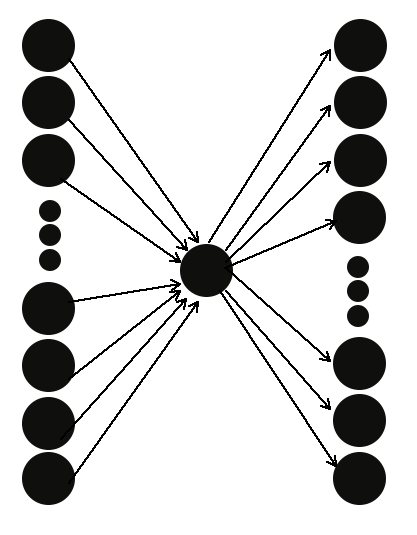
\includegraphics[scale=1]{bowtie2.png}
   \end{center}
   Label the center vertex first, then the $m$ left vertices and finally the $n$
 right vertices, then the adjacency matrix of the bow-tie graph becomes:
 
 $$B =\(
\left(
\begin{array}{c|ccc|ccc}
0       & 0 & \ldots & 0  & 1 & \ldots & 1\\\hline 
1 &  &             &     &    &              & \\
\vdots & & \mathbf{0}_n & && \mathbf{0}&\\
1 &  &             &     &    &              & \\ \hline
0 &  &             &     &    &              & \\
\vdots & & \mathbf{0} & && \mathbf{0}_m&\\
0 & & &     &    &              & \\


\end{array}
\right)
\) $$
 By direct computation, we get that the matrix $B^TB + BB^T$ is equal to:
 $$B^TB + BB^T = \begin{pmatrix}
 m + n & 0 & 0\\
 0 & \mathbf{1}_n & 0\\
 0 & 0 & \mathbf{1}_m
 \end{pmatrix}$$
 By Theorem \ref{centralescore}, the Perron root of $M$ is equal to $\rho = \sqrt{n+m}$ 
 and the similarity matrix is the $(1+m+n)\times 3$-matrix:
 $$S = \frac{1}{\sqrt{m+n+1}}\(
\left(\begin{array}{c|c|c}
 0 & 1 & 0\\\hline
 1 & 0 & 0\\
 \vdots & \vdots & \vdots\\
 1 & 0 & 0\\\hline
 0 & 0 & 1\\
 \vdots & \vdots & \vdots \\
 0 & 0 & 1
 \end{array}\right)
\) $$
 If we see vertex 2 of the path graph $1 \to 2 \to 3$ as the \emph{center}, 
 which can be seen as a vertex through which much information is passed, 
 then it is not surprising that $S$ indicates that vertex $1$ of the directed 
 bow-tie graph is the only one that looks like a center. The left vertices of 
 the bow-tie graph look like vertex 1 of the path graph and the right vertices 
 of the bow-tie graph look like vertex $3$. This is a beautiful example because 
 it confirms our intuition.
 \end{example}
 \subsubsection{Self-similarity of a graph}
When we compute the similarity matrix of two equal graphs $\graf = \grafeen$, 
the similarity matrix $S$ is  square matrix with as entries the similarity 
scores between vertices of $\graf$, we call $S$ the \emph{self-similarity matrix of $\graf$} 
in this case. 

Intuitively, we expect that vertices have the highest similarity scores with 
themselves, which means that the largest entries are located on the diagonal of 
$S$. We prove in the next theorem that the largest entry of a self-similarity 
matrix appears always on the diagonal and that, except for some special cases, 
the diagonal elements of a self-similarity matrix are nonzero. This doesn't mean
that the diagonal elements are always larger than the other elements on the same 
row or column and we conclude this paragraph with some easy examples the show 
this.

\begin{theorem}
  The self-similarity matrix of a graph $\graf$ is positive semidefinite\footnote{A $n\times n$-matrix $A$ is called positive-semidefinite if
$\mathbf{x}^{T} A \mathbf{x}\geq 0$
for all $\mathbf{x}$ in $\R^n$.}. The largest entry of the matrix appears on the 
diagonal and if a diagonal entry is equal to zero,  all the entries of the corresponding row and 
column are also equal to zero.
\end{theorem}
\textbf{Hier ga ik nog enkele relevante eigenschappen van positieve semidefinitie matrices toevoegen, dit bewijs toch net iets te kort door de bocht me dunkt.}
\begin{proof}
  Since A = B, the compact form of Theorem \ref{frobvorm} becomes:
 $$Z^{(k+1)} = \frac{BZ^{(k)}A^T + B^TZ^{(k)}A}{\|BZ^{(k)}A^T + B^TZ^{(k)}A\|_F}, \quad Z^{(0)} = \mathbf{1},  $$
  It is clear that all matrices $Z^{(k)}$ are positive semidefinite because the 
  scaled sum of two positive semidefinite matrices is also positive 
  semidefinite. Since the positive semidefinite matrices form a closed set (in the usual 
  topology), the limit $S$ will also be positive semidefinite. The rest of the 
  theorem are well known properties of positive semidefinite matrices.
\end{proof}
\begin{example}
  The self-similartiy matrix of the graph:
  \begin{center}
  \begin{tikzpicture}[->,>=stealth',shorten >=1pt,auto,node distance=3cm,
                    thick]
                    \tikzstyle{every node}=[draw,circle,fill=black,minimum size=4pt,
                            inner sep=0pt]


  \node[main node] (1) [label=above:$v_1$] {};
  \node[main node] (2) [label=above:$v_2$][right of=1] {};
  \node[main node] (3) [label=above:$v_3$][right of=2] {};;

  \path[every node/.style={font=\sffamily\small}]
   
    (1) edge node [left] {} (2)
      (2) edge node [left] {} (3)
    
\end{tikzpicture}
\end{center}
is equal to:
$$\begin{pmatrix}
  0.5774 & 0 & 0 \\
  0 & 0.5774 & 0 \\
  0 & 0 & 0.5774
\end{pmatrix}$$
\end{example}

\begin{example}
  The self-similartiy matrix of the graph:
  \begin{center}
  \begin{tikzpicture}[->,>=stealth',shorten >=1pt,auto,node distance=3cm,
                    thick]
                    \tikzstyle{every node}=[draw,circle,fill=black,minimum size=4pt,
                            inner sep=0pt]


  \node[main node] (1) [label=above:$v_1$] {};
  \node[main node] (2) [label=left:$v_2$][below left of=1] {};
    \node[main node] (4) [label=right:$v_4$][below right of=1] {};

  \node[main node] (3) [label=below:$v_3$][below right of=2] {};;

  \path[every node/.style={font=\sffamily\small}]
   
    (1) edge node [left] {} (2)
      (2) edge node [left] {} (3)
      (3) edge node [left] {} (4)
      (4) edge node [left] {} (1)
    
\end{tikzpicture}
\end{center}
is equal to:
$$\begin{pmatrix}
  0.250 & 0.250 & 0.250 & 0.250 \\
  0.250 & 0.250 & 0.250 & 0.250 \\
  0.250 & 0.250 & 0.250 & 0.250 \\
  0.250 & 0.250 & 0.250 & 0.250 \\
\end{pmatrix}$$


\end{example}
\begin{example}
  The self-similartiy matrix of the graph:
  \begin{center}
  \begin{tikzpicture}[->,>=stealth',shorten >=1pt,auto,node distance=3cm,
                    thick]
                    \tikzstyle{every node}=[draw,circle,fill=black,minimum size=4pt,
                            inner sep=0pt]


  \node[main node] (1) [label=above:$v_1$] {};
  \node[main node] (2) [label=below:$v_2$][below of=1] {};
    \node[main node] (4) [label=right:$v_4$][below right of=2] {};

  \node[main node] (3) [label=left:$v_3$][below left of=2] {};;

  \path[every node/.style={font=\sffamily\small}]
   
    (1) edge node [left] {} (2)
      (2) edge node [left] {} (3)
      (2) edge node [left] {} (4)
    
\end{tikzpicture}
\end{center}
is equal to:
$$\begin{pmatrix}
  0.4082 & 0 & 0 & 0\\
  0 & 0.4082 & 0 & 0\\
  0 & 0 & 0.4082 & 0.4082\\
    0 & 0 & 0.4082 & 0.4082\\

\end{pmatrix}$$


\end{example}
\section{Node-edge similarity}
The paper of Blondel et al. \cite{blondel} caused a flow of successive papers 
which build upon the concept of similarity between two graphs. For instance, the paper
`Graph similarity scoring and 
matching' of Laura Zager and George Verghese \cite{zager} expands the 
notion of node similarity presented in the previous section to similarity 
between the edges of two graphs. The paper was presented in 2006. Intuitively an 
edge of a graph $\graf$ is similar to an edge of graph $\grafeen$ if their 
\emph{source} and \emph{terminal nodes} are similar. As a consequence, the notion of similarity between edges
introduces a coupling between edge and node similarity scores. The algorithm presented in 
this paper is therefore an extension of the algorithm presented in the previous section.

\subsection{Coupled node-edge similarity scores}
We now present the extended algorithm allowing us to calculate not only a node 
similarity scores, but also edge similarity scores. The algorithm will use a 
new sort of matrices that represent a graph. Recall Definition \ref{terminal} of 
source and terminal nodes.


\begin{definition}
  Let be $\graf=(V,\to)$ be a graph with adjacency matrix A, numbered vertices $v_1, v_2, \ldots, v_n \in V$ 
  and numbered edges $e_1, e_2, \ldots e_m  \in \to$. We define the \textbf{source-edge matrix $A_S$} as a $n\times m$ matrix with entries:
  $$(A_S)_{ij} = \begin{cases} 1 &\mbox{if }s_\graf(e_j) = v_i   \\ 
0 & \mbox{otherwise} \end{cases},$$
the notation $A_S$ is derived from the adjacency matrix $A$.
  \end{definition}
  
  \begin{definition}
  Let be $\graf=(V,\to)$ be a graph with adjacency matrix $A$, numbered vertices $v_1, v_2, \ldots, v_n \in V$ 
  and numbered edges $e_1, e_2, \ldots e_m  \in \to$. We define the \textbf{terminus-edge matrix $A_T$} as a $n\times m$ matrix with entries:
  $$(A_T)_{ij} = \begin{cases} 1 &\mbox{if }$t_\graf(e_j) = v_i$   \\ 
0 & \mbox{otherwise} \end{cases},$$
the notation $A_T$ is derived from the adjacency matrix $A$.  \end{definition}
\begin{property}\label{outdegreeprop}
Let $\graf=(V,\to)$ be a graph, then $A_SA^T_S$ is a diagonal matrix where the $i$th diagonal entry is equal the outdegree of vertex $v_i$.
   \end{property}
   \begin{proof}
By direct computation, we get:
$$(A_SA_S^T)_{ij} = \sum^m_{k=1}(A_S)_{ik}(A_S)^T_{kj} = \sum^m_{k=1}(A_S)_{ik}(A_S)_{jk}$$
Assume $i \not = j$. Then for each $k$, $(A_S)_{ik}(A_S)_{jk}= 0$ since vetrex $v_i$ 
and vertex $v_j$ can't be both the source node of edge $k$.

When $i=j$, then for each $k$, $(A_S)_{ik}(A_S)_{jk}= ((A_S)_{ik})^2$ equals 0 or 1 depending on whether $v_i$ 
is a starting point or not, so 1 is added to $(A_SA_S^T)_{ii}$ each time an edge `departs' from 
$v_i$, this is exactly the outdegree of vertex $v_i$.
   \end{proof}
   
In an analogous way, we prove:
\begin{property}\label{indegreeprop}
Let $\graf=(V,\to)$ be a graph, then $A_TA_T^T$ is a diagonal matrix where the $i$th diagonal entry is equal the indegree of vertex $v_i$.
   \end{property}

\begin{property}\label{adjacencyprop}
  Let $\graf =(V,\to)$ be a graph, then the adjacency matrix $A$ is equal to 
  $A_SA^T_T$.
\end{property}
\begin{proof}
  By direct computation, we get:
  $$(A_SA_T^T)_{ij} = \sum^m_{k=1}(A_S)_{ik}(A_T)^T_{kj} = \sum^m_{k=1}(A_S)_{ik}(A_T)_{jk}$$
The terms $(A_S)_{ik}(A_T)_{jk}$ equal $1$ if edge $k$ goes from $v_i$ to 
$v_j$ and since the sum is taken over all edges we conclude:
$$(A_SA_T^T)_{ij} = A_{ij}.$$
\end{proof}
Let  $\graf(V,\to)$, $\grafeen(U,\to')$ be two (directed) graphs, $\graf$ has $n_\graf$ vertices and $m_\graf$ edges and $\grafeen$ has $n_\grafeen$ vertices and $m_\grafeen$. 
Remember the following updating equation from (\ref{vergblondel}), which returns the 
(node) similarity score between vertices $u_i$ 
from $\grafeen$ and $v_j$ from $\graf$:
\begin{eqnarray*}
 x^{(k+1)}_{ij} = \sum_{r:(u_r,u_i)\in \to', w:(v_w,v_j) \in \to} x^{(k)}_{rw} +  \sum_{r:(u_i,u_r)\in \to', w:(v_j,v_w) \in \to} 
 x^{(k)}_{rw},
 \end{eqnarray*} 
if we number the edges of $\graf$ and $\grafeen$ as  $e_1, e_2, \ldots e_{m_\graf}  \in \to$ and $e'_1, e'_2, \ldots, e'_{m_\grafeen}  \in \to'$, this can be rewritten as:
 \begin{eqnarray*}
 x^{(k+1)}_{ij} = \sum_{t_\grafeen(e'_p)=u_i, t_\graf(e_q)=v_j} x^{(k)}_{s_\grafeen(e'_p)s_\graf(e_q)} +  \sum_{s_\grafeen(e'_p)=u_i, s_\graf(e_q)=v_j} 
 x^{(k)}_{t_\grafeen(e'_p)t_\graf(e_q)}.
 \end{eqnarray*} 
 We now extend this mutually reinforcing relation with the notion of edge 
 similarity. $x_{ij}$ denotes again the node similarity score between vertex $u_i$ from $\grafeen$ and vertex $v_j$ from $\graf$ 
 and $y_{pq}$ denotes the edge similarity score between edge $p$ from $\grafeen$ and edge $q$ in $\graf$, the update equations for edge and node similarity scores take now the 
 following form:
 \begin{eqnarray}
 y_{pq}^{(k+1)} &=& x^{(k)}_{s_\grafeen(e'_p)s_\graf(e_q)} + x^{(k)}_{t_\grafeen(e'_p)t_\graf(e_q)}\label{edge1}\\
 x^{(k+1)}_{ij} &=& \sum_{t_\grafeen(e'_r)=u_i, t_\graf(e_w)=v_j} y^{(k)}_{rw} +  \sum_{s_\grafeen(e_t)=u_i, s_\graf(e_w)=v_j} y^{(k)}_{rw} \label{edge2}
 \end{eqnarray} 
With the same 
 reasoning as presented in the previous section, these scores can be assembled into matrices $Y^{(k)}$ and $X^{(k)}$ 
by using the source-edge matrices $A_S$ and the terminus-edge matrices $A_T$. Let $A$ be the adjacency matrix of $\graf$ and $B$ be the adjacency
matrix of $\grafeen$, let $X^{(k)}$ be the $n_\grafeen \times n_\graf$-matrix with entries $x_{ij}$, the node similarity scores at iteration step $k$ 
and let $Y^{(k)}$ be the $m_\grafeen \times m_\graf$-matrix with entries $y_{pq}$, the edge similarity scores at step $k$. The equations (\ref{edge1}) and (\ref{edge2}) 
can be rewritten as:
\begin{eqnarray}
  Y'^{(k+1)} &=& B_S^TX^{(k)}A_S + B_T^TX^{(k)}A_T\label{edgematrix1}\\
   X'^{(k+1)} &=& B_SY^{(k)}A_S^T + B_TY^{(k)}A^T_T\label{edgematrix2}
 \end{eqnarray}
 for  $k =  0,1,\ldots$
 
 Of course we want to customize these equations in a way that we can apply Theorem \ref{grootbewijs} to prove convergence. 
 This will be completely analogous to Theorem \ref{frobvorm}, but we can achieve a slightly better result: not only the even and odd iterates
 will converge, the iteration converges as a whole. Lastly, remember that one of the conditions of Theorem \ref{grootbewijs} is to 
 normalize the results at each iteration step. Therefore, the following theorem comes as no surprise:

 \begin{theorem}\label{edgegrootbewijs}
   Let $\graf$ and $\grafeen$ be two graphs with adjacency matrices $A$ and $B$, $\graf$ has $n_\graf$ vertices and
   $m_\graf$ edges and $\grafeen$ has $n_\grafeen$ vertices and $m_\grafeen$ edges, define: 


   
 \begin{eqnarray}
  Y^{(k+1)} &=& \frac{B_S^TX^{(k)}A_S + B_T^TX^{(k)}A_T}{\|B_S^TX^{(k)}A_S + 
  B_T^TX^{(k)}A_T\|_F}\label{edgegroot1}\\
   X^{(k+1)} &=& \frac{B_SY^{(k)}A_S^T + B_TY^{(k)}A^T_T}{\|B_SY^{(k)}A_S^T + 
   B'_TY^{(k)}A^T_T\|_F}\label{edgegroot2}
 \end{eqnarray}
  for  $k =  0,1,\ldots$.
  
  Then the matrix subsequences $X^{(2k)}$, $Y^{(2k)}$ and $X^{(k+1)}$, $Y^{(k+1)}$ 
  converge to $X_{\text{even}}$, $Y_{\text{even}}$ and $X_{\text{odd}}$, 
  $Y_{\text{odd}}$. If we take\footnote{$J$ is a matrix of all ones}:
  \begin{eqnarray*}  X^{(0)} = J \in \R^{n_\grafeen \times n_\graf}\\
    Y^{(0)} = J \in \R^{m_\grafeen \times m_\graf}
  \end{eqnarray*}
 as initial matrices, then $X_{\text{even}}(\mathbf{1})=X_{\text{odd}}(\mathbf{1})$, $Y_{\text{even}}(\mathbf{1})= Y_{\text{odd}}(\mathbf{1})$ 
 are the unique matrices of largest 1-norm among all possible limits with positive 
 initial matices and the matrix sequence $X^{(k)}$, $Y^{(k)}$ converges has a 
 whole.
  \end{theorem}
  \begin{proof}
 By Theorem \ref{tensor} we can rewrite (\ref{edgematrix1}) as follows:
 \begin{eqnarray*}
         Y'^{(k+1)} &=& B_S^TX'^{(k)}A_S + B_T^TX'^{(k)}A_T\\
  \Leftrightarrow  \vect(Y'^{(k+1)}) &=& \vect(B_S^TX'^{(k)}A_S + 
  B_T^TX'^{(k)}A_T)\\
  \Leftrightarrow  \vect(Y'^{(k+1)}) &=& \vect(B_S^TX'^{(k)}A_S) + 
  \vect(B_T^TX'^{(k)}A_T)\\
  \Leftrightarrow \vect(Y'^{(k+1)}) &=& (A_S^T \otimes B_S^T)\vect(X'^{(k)}) + (A^T_T \otimes 
  B^T_T)\vect(X'^{(k)})\\
   \Leftrightarrow \vect(Y'^{(k+1)}) &=& (A_S^T \otimes B_S^T + A^T_T \otimes 
  B^T_T)\vect(X'^{(k)})
 \end{eqnarray*}
 Completely analogously we can also rewrite (\ref{edgematrix2}):
 $$\vect(X'^{(k+1)}) &=& (A_S \otimes B_S + A_T \otimes B_T)\vect(Y^{k}),$$
 define $\mathbf{y}^{(k)}=\vect(Y'^{(k+1)})$ and $\mathbf{x}^{(k)}= \vect(X'^{(k+1)})$, we get:
 \begin{eqnarray*}
   \mathbf{y}^{(k+1)} &=& (A_S^T \otimes B_S^T + A^T_T \otimes 
   B^T_T)\mathbf{x}^{(k)}\\
   \mathbf{x}^{(k+1)} &=& (A_S \otimes B_S + A_T \otimes B_T)\mathbf{y}^{(k)}
 \end{eqnarray*} 
 If we define $G = A_S^T \otimes B_S^T + A^T_T \otimes B^T_T$, then with Lemma \ref{hulptensor} and well known
 properties of transpose matrices:
 \begin{eqnarray*}
   G^T &=& (A_S^T \otimes B_S^T + A^T_T \otimes B^T_T)^T\\
   &=& ((A_S\otimes B_S)^T + (A_T \otimes B_T)^T)^T\\
   &=& ((A_S\otimes B_S)^T)^T +  ((A_T \otimes B_T)^T)^T\\
   &=& A_S\otimes B_S + A_T \otimes B_T
 \end{eqnarray*}
 So we get:
  \begin{eqnarray}
     \mathbf{y}^{(k+1)} &=& G\mathbf{x}^{(k)}\label{uitgeschrevenvectoren1}\\
     \mathbf{x}^{(k+1)} &=& G^T\mathbf{y}^{(k)}\label{uitgeschrevenvectoren2},
 \end{eqnarray}
$G$ is a $m_\graf m_\grafeen \times n_\graf n_\grafeen$-matrix, the previous expressions  can be concatenated to a single matrix update equation (we define matrix $M$ and $\mathbf{z}^{(k+1)}$):
 $$\mathbf{z}^{(k+1)} =\begin{pmatrix}
 \mathbf{x}\\
 \mathbf{y}
 \end{pmatrix}^{(k+1)} = \begin{pmatrix}
 \mathbf{0}_{m_\graf m_\grafeen} & G^T\\
 G & \mathbf{0}_{n_\graf n_\grafeen} \\
 \end{pmatrix}
 \begin{pmatrix}
 \mathbf{x}\\
 \mathbf{y}
 \end{pmatrix}^{(k)}
 = M\mathbf{z}^{(k)},$$
$M$ is clearly nonnegative because $G$ and $G^T$ consists of sums of Kronecker products of $A_S, B_S, A_T$ and/or $B_T$, all matrices
 with entries equal to zero or one, $M$ is as a $(n_\graf n_\grafeen + m_\graf m_\grafeen)\times(n_\graf n_\grafeen + m_\graf m_\grafeen)$-matrix
 clearly symmetric, so the result follows immediately from Theorem \ref{grootbewijs}. 
The appearance of the Perron norm can be explained in the same way as in Theorem \ref{frobvorm}, note that we write $Y^{(k)}$ and $X^{(k)}$ 
for the normalized results at iteration step $k$. We still have to prove that 
odd and even iterates are the same and that $M$ has only positive eigenvalues, meaning that the sequence converges to $\frac{\Pi \mathbf{z}^{(0)}}{\|\Pi \mathbf{z}^{(0)}\|_2}$,
this can be done easily by expanding the matrix equation: 
$$\mathbf{x}^{(k)} = \begin{cases} 
(G^TG)^{\frac{k}{2}}\mathbf{x}^{(0)  &\mbox{k even }\\
 
(G^TG)^{\frac{k-1}{2}}G^T\mathbf{y}^{(0)&\mbox{k odd}
\end{cases} \quad \text{and} \quad
\mathbf{y}^{(k)} = \begin{cases} 
(GG^T)^{\frac{k}{2}}\mathbf{y}^{(0)  &\mbox{k even }\\
 
(GG^T)^{\frac{k-1}{2}}G\mathbf{x}^{(0)&\mbox{k odd}
\end{cases}
$$
The matrix $G$ is the sum of two matrices $(A_S^T \otimes B_S^T)$ and $(A^T_T \otimes 
B^T_T)$. Now, $A_S^T$ is a $m_\graf \times n_\graf$-matrix and has in each row a 
single `$1$'-entry, simply because an edge has at most one source node . The same holds for 
$B_S^T$. Therefore, taking the Kronecker product of those two matrices results in the matrix $A_S^T \otimes B_S^T$
which also has just a single `$1$' entry in each row. With the same reasoning, 
we conclude that also $A^T_T \otimes B^T_T$ has also just a single `$1$'-entry in each row. Taking 
the sum of $(A_S^T \otimes B_S^T)$ and $(A^T_T \otimes 
B^T_T)$ results thus in the matrix $G$ with exactly two $1$ entries in each row. If we now choose the initial conditions as 
$\mathbf{x}^{(0)} = \mathbf{1} \in \R^{n_\grafeen n_\graf}$ and $\mathbf{y}^{(0)} = 
\mathbf{1} \in \R^{m_\grafeen m_\graf}$, we conclude:
$$G\mathbf{x}^{(0)} = 2\mathbf{y}^{(0)},$$
we get:
\begin{eqnarray*}
\mathbf{x}^{(k)} &=& \begin{cases} 
(G^TG)^{\frac{k-2}{2}}G^TG\mathbf{x}^{(0)} = \frac{1}{2}(G^TG)^{\frac{k-2}{2}}G^T\mathbf{y}^{(0) &\mbox{$k$ even }\\
(G^TG)^{\frac{k-1}{2}}G^T\mathbf{y}^{(0)&\mbox{$k$ odd}
\end{cases}\\
\mathbf{y}^{(k)} &=& \begin{cases} 
(GG^T)^{\frac{k}{2}}\mathbf{y}^{(0)  &\mbox{$k$ even }\\
(GG^T)^{\frac{k-1}{2}}G\mathbf{x}^{(0)} = (GG^T)^{\frac{k-1}{2}}\frac{1}{2}\mathbf{y}^{(0)\;\;\;\;\;\;\;\;\;\;\;\;\;&\mbox{$k$ odd}
\end{cases}
\end{eqnarray*}
First, observe that the matrices $GG^T$ and $G^TG$ are besides being symmetric (for example, $(GG^T)^T = GG^T$) 
and nonnegative, are also positive semi-definite and thus have only nonnegative 
eigenvalues. Note that the factor $\frac{1}{2}$ that appears in the odd iterates 
will be eliminated by the normalization in each step. So in the limit as $k \to \infty$ 
, the even and odd iterates are the same.

 \end{proof}
 We now define $X_{\text{even}}(\mathbf{1})$ as the node similarity matrix and $Y_{\text{even}}(\mathbf{1})$ as the edge similarity 
 matrix.
 
 
 

  \subsection{The algorithm}
  \begin{algorithm}[h!]\label{edgealgorithm}
 \KwData{\\
 $A_S$:  the $n_\graf \times m_\graf$ source-edge matrix of a graph $\graf$\\
 $A_T$:  the $n_\graf \times m_\graf$ terminal-edge matrix of a graph $\graf$\\
 $B_S$: the $n_\grafeen \times m_\grafeen$ source-edge matrix of a graph $\graf$\\
 $B_T$: the $n_\grafeen \times m_\grafeen$ terminal-edge matrix of a graph $\graf$\\
 $\tol$: tolerance for the estimation error.\\
 \KwResult{\\
 $X$: the node similarity matrix between $\graf$ and $\grafeen$\\
 $Y$: the edge similarity matrix between $\graf$ and $\grafeen$}
 \blankline
\SetKwFunction{powermethod}{node\_edge\_similarity\_matrix}
\SetKwFunction{hits}{hits}

\SetKwProg{myalg}{begin}{}{end}
\myalg{\powermethod{$A_S$,$A_T$, $B_S$,$B_T$,$\tol$}}{
$k = 1$ \;
$X^{(0)} = \mathbf{1}$ ($n_\grafeen\times n_\graf$-matrix with all entries equal to $1$)\;
$Y^{(0)} = \mathbf{1}$ ($m_\grafeen\times m_\graf$-matrix with all entries equal to $1$)\;
$\mu_X =  n_\grafeen\times n_\graf$-matrix with all entries equal to $\tol$\;
$\mu_Y =  m_\grafeen\times m_\graf$-matrix with all entries equal to $\tol$\;

\Repeat{$|X^{(k)} - X^{(k-1)}| < \mu_X$ and $|Y^{(k)} - Y^{(k-1)}| < \mu_Y$ }{
$Y^{(k)}=& \frac{B_S^TX^{(k-1)}A_S + B_T^TX^{(k-1)}A_T}{\|B_S^TX^{(k-1)}A_S + B_T^TX^{(k-1)}A_T\|_F}$\;
$X^{(k)} = \frac{B_SY^{(k)}A_S^T + B_TY^{(k)}A^T_T}{\|B_SY^{(k)}A_S^T + B'_TY^{(k)}A^T_T\|_F}$\;
$k = k + 1$\;
}
 
\KwRet $X^{(k)}, Y^{(k)} $\;}{}
  \caption{Algorithm for calculating the node and edge similarity matrix $X$ and $Y$ between $\graf$ and $\grafeen$.\\}\label{edgealgorithm}
\end{algorithm}\label{edgealgorithm}
 
 The algorithm to calculate the node and edge similarity scores is presented in pseudo-code in Algorithm \ref{edgealgorithm}. 
 Remember that the absolute value that is mentioned is the same as in Notation 
 \ref{modulusmatrix}. Besides the different calculations, the main difference with the algorithm of the previous section (Algorithm \ref{algsimilarity})
 is that the whole sequence converges, not only the even (or odd) iterates, 
 making this algorithm twice as fast. This is because in Algorithm \ref{algsimilarity} we take the limit
 of the even iterates but we need the calculations of the odd iterates too to achieve a result. In this
 implementation, the algorithm will not oscillate and both the even and odd iterates converge to the same limit, so the tolerance level will
 be satisfied with half of the number of steps we would need for Algorithm \ref{algsimilarity}. Also notice that we implement a \textit{sequential} 
 update: when $Y^{(k)}$ is calculated,the result is immediately used in 
 $X^{(k)}$. This is not according to Theorem \ref{edgegrootbewijs}, which 
 suggest \textit{simultaneous} updating equations: in that case $X^{(k)}$ uses $Y^{(k-1)}$ 
 in it's calculations. It is not difficult to see, by an analogous argument of 
 Theorem \ref{edgegrootbewijs}, that both approaches yield the same set of 
 similarity scores. Numerical analysts, however, will always prefer the sequential
 update procedure because it performs slightly better (see section 3.2 in \cite{numeriekwiskunde}) as you directly use a more accurate 
 result for $Y^{(k)}$ in the calculation of $X^{(k)}$. 
 
 A Matlab implementation 
 can be found in Listing \ref{edgematlab} in Appendix \ref{appendixa}. Because giving source-edge matrices and terminal-edge matrices as input
 is quite unnatural, in Listing \ref{sourceedgematlab} and Listing \ref{terminaledgematlab} 
 some Matlab code is also presented to transform an adjacency matrix into a 
 source-edge matrix and a terminal-edge matrix. The resulting matrices represent an edge numbering left-to-right, based on the entries of the adjacency matrix. The algorithm to calculate the 
 source-edge matrix based on the adjacency matrix is also written in pseudo-code in Algorithm 
 \ref{sourceedge}, the calculation of the terminal-edge matrix is completely 
 analogous. A Matlab implementation of Algorithm \ref{edgealgorithm} that takes 
 two adjacency matrices as input can be found in Listing \ref{zeeruitgebreid}.
 
   \begin{algorithm}[H]\label{sourcedge}
 \KwData{\\
 $A$:  the $n \times n$ adjacency matrix of a graph $\graf$\\
 \KwResult{\\
 $A_S$: the source-edge matrix of graph $\graf$}
 \blankline
\SetKwFunction{powermethod}{source\_edge\_matrix}
\SetKwFunction{hits}{hits}

\SetKwProg{myalg}{begin}{}{end}
\myalg{\powermethod{$A$}}{
$m$ = sum of all entries of $A$ \;
$A_S$ = initialize a $n \times m$-matrix with all entries equal to 0\;
current\_edge = 1\;

\For{$i: 1$ to $n$ }{
  \For{$j: 1$ to $n$ }{
     \If{$(A)_{ij} > 0$}{
          \For{$e: 1$ to $(A)_{ij}$}{
            $(A_S)_{i, \text{current\_edge }}$ = 1\;
            current\_edge = current\_edge + 1 \;
          }
     }
  }}}
 
\KwRet $A_S$\;}{}
  \caption{Algorithm for calculating the source-edge matrix $A_S$ based on the adjacency matrix $A$ of a graph $\graf$.\\}\label{sourceedge}
\end{algorithm}
 
 \subsection{Difference with node similarity}
It is clear that the node-edge similarity algorithm is different from 
Algorithm \ref{algsimilarity} from the previous section. We will make this a little 
more explicit and show the difference in the resulting node similarity matrix. We first need another property of the Kronecker 
product.

\begin{property}\textbf{(mixed-product property of Kronecker products)}
  Let $A \in \R^{m\times n}, B \in \R^{r \times s}, C \in \R^{n\times p}$ and $D \in \R^{s \times t}$ 
  then:
  $$(A\otimes B)(C \otimes D) = AC \otimes BD$$
\end{property}
\begin{proof}
  \begin{eqnarray*}
(A\otimes B)(C \otimes D) &=&
  \begin{pmatrix}
    a_{11}B & \ldots & a_{1n}B\\
    \vdots & \ddots & \vdots\\
    a_{m1}B & \ldots & a_{mn}B
  \end{pmatrix}
  \begin{pmatrix}
    c_{11}D & \ldots & c_{1p}D\\
    \vdots & \ddots & \vdots\\
    a_{n1}D & \ldots & a_{np}D
  \end{pmatrix}\\
  &=& \begin{pmatrix}
    \sum_{k=1}^n a_{1k}c_{k1}BD & \ldots & \sum_{k=1}^n a_{1k}c_{kp}BD\\
    \vdots & \ddots & \vdots\\
    \sum_{k=1}^n a_{mk}c_{k1}BD & \ldots & \sum_{k=1}^n a_{mk}c_{kp}BD\\
  \end{pmatrix}\\
  &=& AC \otimes BD.
  \end{eqnarray*}
\end{proof}



Now take equations (\ref{uitgeschrevenvectoren1}) and 
(\ref{uitgeschrevenvectoren2}) and consider only the even iterates. We consider only the even iterates because Algorithm \ref{algsimilarity} does, 
remember that in Algorithm \ref{edgealgorithm} the even and odd iterates yield 
the same set of similarity scores. We get:
\begin{eqnarray*}
  \mathbf{x}^{(k)} &=& (G^TG)\mathbf{x}^{(k-2)}\\
  &=& ((A_S\otimes B_S + A_T \otimes B_T)(A^T_S \otimes B^T_S + A^T_T \otimes 
  B^T_T))\mathbf{x}^{(k-2)}\\
  &=& ((A_S\otimes B_S)(A^T_S \otimes B^T_S) + (A_S\otimes B_S)(A^T_T \otimes 
  B^T_T) \\
  &\quad& + (A_T \otimes B_T)(A^T_S \otimes B^T_S) + (A_T \otimes B_T)(A^T_T \otimes 
  B^T_T))\mathbf{x}^{(k-2)}\\
  &=& (A_S A^T_S \otimes B_SB^T_S + A_SA^T_T \otimes B_SB^T_T \\
  &\quad& + A_TA^T_S \otimes 
  B_TB^T_S + A_TA^T_T\otimes B_TB^T_T)\mathbf{x}^{(k-2)}\\
  &=& (A_S A^T_S \otimes B_SB^T_S + A \otimes B + A^T \otimes B^T + A_TA^T_T\otimes 
  B_TB^T_T)\mathbf{x}^{(k-2)}\\
  &=& (A \otimes B + A^T \otimes B^T + A_S A^T_S \otimes B_SB^T_S + A_TA^T_T\otimes 
  B_TB^T_T)\mathbf{x}^{(k-2)}
\end{eqnarray*}
Where $A, B$ are the adjacency matrices of $\graf, \grafeen$ (Property 
\ref{adjacencyprop}), 
$A_S A^T_S, B_S B^T_S$ are the diagonal matrices with the outdegrees of the vertices 
on the diagonal (Property \ref{outdegreeprop}) and $A_TA^T_T, 
  B_TB^T_T$ are the diagonal matrices with the indegree of the vertices on the 
  diagonal (Property \ref{indegreeprop}). The iteration sugested in Theorem \ref{frobvorm} 
  in the previous section has the following form (see equation 
  (\ref{uitgeschrevenvectornormaal})):
  $$\mathbf{x}^{(k)} = A \otimes B + A^T \otimes B^T\mathbf{x}^{(k-2)},$$
thus Algorithm \ref{edgealgorithm} differs from Algorithm \ref{algsimilarity} in three important ways:
\begin{itemize}
  \item  In Algorithm \ref{edgealgorithm} the inclusion of additional diagonal terms serve to amplify the scores of 
nodes that are highly connected in the node similarity matrix,
\item  Algorithm \ref{edgealgorithm} returns a node similarity matrix and an edge similarity matrix, Algorithm \ref{algsimilarity}
returns only a node similarity matrix,
\item The whole sequence in Algorithm \ref{edgealgorithm} converges, not only 
the even and odd iterates.

\end{itemize}
  
  
 \subsection{Example}
 \begin{example}
   We retake Example \ref{eenvoudigvoorbeeldjes} and number the edges as 
   follows, let $\graf = (V,\to)$ be :
\begin{center}
\begin{tikzpicture}[->,>=stealth',shorten >=1pt,auto,node distance=3cm,
                    thick]
                    \tikzstyle{every node}=[draw,circle,fill=black,minimum size=4pt,
                            inner sep=0pt]


  \node[main node] (1) [label=above:$v_1$] {};
  \node[main node] (2) [label=above:$v_2$][right of=1] {};
  \node[main node] (3) [label=above:$v_3$][right of=2] {};;

  \path[every node/.style={font=\sffamily\small}]
   
    (1) edge node [above] {1} (2)
      (2) edge node [above] {2} (3)
    
\end{tikzpicture}
\end{center}
Let $\grafeen=(W,\to)$ be the following graph:
 \begin{center}
\begin{tikzpicture}[->,>=stealth',shorten >=1pt,auto,node distance=3cm,
                    thick]
                    \tikzstyle{every node}=[draw,circle,fill=black,minimum size=4pt,
                            inner sep=0pt]

 \node[main node] (1) [label=above:$w_1$] {};

  \node[main node] (2) [label=left:$w_2$] [below left of =1; left of=3]{};
  \node[main node] (3) [label=right:$w_3$][below right of=1;] {};
    \node[main node] (4) [label=left:$w_4$][below of=2] {};
  \node[main node] (5) [label=right:$w_5$][below of=3] {};
  \path[every node/.style={font=\sffamily\small}]
       (1) edge node [left] {$1$} (2)
      (1) edge node [right] {$2$} (3)
      (2) edge node [near start, below] {$5$} (5)
            (2) edge node [above] {$3$} (3)

      (2) edge node [left] {$4$} (4)
      (3) edge node [near start] {$6$} (4)
      (3) edge node [right] {$7$} (5)

\end{tikzpicture}
\end{center}
Then the node similarity matrix is:

$$X = \begin{pmatrix}
0.2338  &  0.0718  &       0\\
0.2472   & 0.3230  &  0.0128\\
0.1841   &  0.7553 &   0.3185\\
0  &  0.0935  &  0.2338\\
0   & 0.0441 &   0.0576
\end{pmatrix},$$
 and the edge similarity matrix equals:
 $$ Y = \begin{pmatrix}
0.2166 & 0.0329\\
0.3847 & 0.1518\\
0.3899 & 0.2495\\
0.1325 & 0.2166\\
0.1133 & 0.1480\\
0.3653 & 0.4176\\
0.1080 & 0.3847
\end{pmatrix}$$
If you look at the structure of $\grafeen$ and compare it with the structure of $\graf$, then 
intuitively it is not surprising that edge $3$ of $\grafeen$ is most similar to edge $1$ of 
$\graf$ and edge $6$ of $\grafeen$ is most similar to edge $2$ of $\graf$ because they are both very
central edges with source nodes and terminal nodes that are very similar.
 \end{example}
 


\section{Colored graphs}
In this last section, we extend the notion of similarity to colored graphs. The 
paper \cite{vandoren} is written by two Belgian professors Paul Van Dooren and 
Catherine Fraikin from the Catholic University of 
Louvain in 2009.

Graph coloring is already introduced in paragraph \ref{colored} and we will 
construct a method that returns similarity matrices for two graphs where the coloring is on the nodes or 
on the edges of both graphs. If you would compare the orignal paper to 
explanation in this section, you will see that there are lot of differences. 
This has two reasons: first, with the previous sections we have already a broad overview of 
similarity on graphs so we can achieve results in a more detailed way, second, to make 
the notations uniform in the whole master thesis, this paper had to be 
rewritten.


\subsection{Colored nodes}
We first extend the node similarity introduced in section \ref{sectionnodesim} to 
node colored graphs. Take two node colored graphs $\graf=(V,\to, C, a)$ and $\grafeen=(U,\to', C, a')$ with $|C|$ (remember that $a$, $a'$ are surjective) different colors and assume that the nodes 
in both graphs are renumbered such that those of color $1$ come first, then 
those of color $2$,... The adjacency matrices $A$ (of graph $\graf$) and $B$ (of graph $\grafeen$) 
can then be partitioned as follows:
$$A = \begin{pmatrix}
A_{11} & A_{12} & \ldots & A_{1|C|}\\
A_{11} & A_{12} & \ldots & A_{1|C|}\\
\vdots & \vdots & \ddots & \vdots\\
A_{|C|1} & A_{|C|2} & \ldots & A_{|C||C|}\\
\end{pmatrix}
 \quad \text{and} \quad
 \begin{pmatrix}
B_{11} & B_{12} & \ldots & B_{1|C|}\\
B_{11} & B_{12} & \ldots & B_{1|C|}\\
\vdots & \vdots & \ddots & \vdots\\
B_{|C|1} & B_{|C|2} & \ldots & B_{|C||C|}\\
\end{pmatrix}$$
Remember that $c_\graf(V,i)$ denotes the number of vertices of color $i$ in graph $\graf$, then each block $A_{ij} \in \R^{c_\graf(V,i)\times c_\graf(V,j)}$ and $B_{ij} \in \R^{c_\grafeen(U,i)\times c_\grafeen(U,j)}$ 
describes the adjacency relations between the nodes of color $i$ to the vertices 
of color $j$ in both $A$ and $B$. In fact, by just renumbering the vertices such 
that the nodes with the same color succeed each other, you immediately get such 
partitioning. If you see this renumbering as a permutation on the nodes,
then performing on the original adjacency matrix a left and right multiplication with the corresponding permutation matrix (see Definition 
\ref{petmruation}) leads to this adjusted adjacency matrix.
To make the idea more comprehensible, we give an example.

\begin{example}
  Let $\graf$ be following graph:
  \begin{center}
\begin{tikzpicture}[->,>=stealth',shorten >=1pt,auto,node distance=3cm,
                    thick]
                    \tikzstyle{every node}=[draw,circle,fill=black,minimum size=6pt,
                            inner sep=0pt]


  \node[main node, fill=green] (1) [label=below:$v_1$] {};
  \node[main node, fill=blue] (2) [label=below:$v_2$][right of=1] {};
  \node[main node, fill=green] (3) [label=below:$v_3$][right of=2] {};;
  \node[main node, fill=yellow] (4) [label=below:$v_4$][right of=3] {};;

  \path[every node/.style={font=\sffamily\small}]
   
    (1) edge node [above] {} (2)
    (1) edge[bend right=30]  node [below] {} (3)

    (2) edge node [above] {} (3)
     (3) edge node [above] {} (4)
     (3) edge [bend right=30] node [below] {} (4)
     (2) edge [bend left=40] node [above] {} (3)
     (3) edge [bend right=40] node [above] {} (2)
     (4) edge [loop above] node {} (4)
\end{tikzpicture}
\end{center}
The adjacency matrix equals:
$$A = \begin{pmatrix}
0 & 1 & 1  & 0\\
0 & 0 & 2 & 0\\
0 & 1 & 0 & 2\\
0 & 0 & 0 & 1\\
\end{pmatrix}.$$
If we order the colors as: $\{\text{green, blue, yellow}\}$ (so color 1 = green, color 2 = blue, color 3 = yellow), we can renumber the 
vertices and get the following graph:
\begin{center}
\begin{tikzpicture}[->,>=stealth',shorten >=1pt,auto,node distance=3cm,
                    thick]
                    \tikzstyle{every node}=[draw,circle,fill=black,minimum size=6pt,
                            inner sep=0pt]


  \node[main node, fill=green] (1) [label=below:$v_1$] {};
  \node[main node, fill=green] (2) [label=below:$v_2$][right of=1] {};
  \node[main node, fill=blue] (3) [label=below:$v_3$][right of=2] {};;
  \node[main node, fill=yellow] (4) [label=below:$v_4$][right of=3] {};;

  \path[every node/.style={font=\sffamily\small}]
    (1) edge[bend right=30] node [below] {} (3)
    (1) edge node [below] {} (2)

    (3) edge node [above] {} (2)
     (2) edge[bend right=30] node [below] {} (4)
     (2) edge[bend right=20] node [below] {} (4)
        (2) edge [bend left=40] node [above] {} (3)
     (3) edge [bend right=40] node [above] {} (2)
          (4) edge [loop above] node {} (4)

\end{tikzpicture}
\end{center}

The adjacency matrix equals:
$$A' = PAP = \begin{pmatrix}
1 & 0 & 0 & 0\\
0 & 0 & 1 & 0\\
0 & 1 & 0 & 0\\
0 & 0 & 0 & 1
\end{pmatrix}\begin{pmatrix}
0 & 1 & 1  & 0\\
0 & 0 & 2 & 0\\
0 & 1 & 0 & 2\\
0 & 0 & 0 & 1\\
\end{pmatrix}\begin{pmatrix}
1 & 0 & 0 & 0\\
0 & 0 & 1 & 0\\
0 & 1 & 0 & 0\\
0 & 0 & 0 & 1
\end{pmatrix}=
\begin{pmatrix}
0 & 1 & 1 & 0\\
0 & 0 & 1 & 2\\
0 & 2 & 0 & 0\\
0 & 0 & 0 & 1
\end{pmatrix},$$
which can be partitioned in blocks as follows (we have 3 colors: 1 = green, 2 = blue, 3 = yellow):
$$A' = \begin{pmatrix}
A_{11} & A_{12} & A_{13}\\
A_{21} & A_{22} & A_{23}\\
A_{31} & A_{32} & A_{33}\\
\end{pmatrix} =
\begin{pmatrix}\smallskip
\begin{pmatrix}
 0 & 1\\
 0 & 0\\
\end{pmatrix}& 
\begin{pmatrix}
 1\\
 1\\
\end{pmatrix}
& \begin{pmatrix}
0\\
2\\
\end{pmatrix}\\ \smallskip
 \begin{pmatrix}
0 & 2\\
\end{pmatrix} & \begin{pmatrix}
 0\\
\end{pmatrix} & \begin{pmatrix}
 0\\
\end{pmatrix}\\
\begin{pmatrix}
 0 & 0\\
\end{pmatrix} & \begin{pmatrix}
 0\\
\end{pmatrix} & \begin{pmatrix}
 1\\
\end{pmatrix}\\
\end{pmatrix} .$$
\end{example}
Now, we will only compare the nodes of the same color in both graphs, so that we 
define similarity matrices $S_{ii} \in \R^{c_\graf(V,i)\times c_\grafeen(v_i)}$, with 
$i=1,\ldots,|C|$, which we can put in a block-diagonal similarity matrix:
$$S = \begin{pmatrix}
S_{11} & 0 & \ldots & 0\\
0 & S_{12} & \ldots & 0\\
\vdots & \vdots & \ddots & \vdots\\
0 & 0 & \ldots & S_{|C||C|}
\end{pmatrix}$$



\begin{theorem}
  Let $\graf=(V,\to, C, a)$ and $\grafeen=(U,\to', C, a')$ be two node colored graphs and define:
  \begin{eqnarray*}
  Z^{(k+1)}_1 &=& \sum_{i \in \{1,\ldots, |C|\}}B_{1i}S^{(k)}_{ii}A^T_{1i} + B^T_{i1}S^{(k)}_{ii}A_{i1}\\
  Z^{(k+1)}_2 &=& \sum_{i \in \{1,\ldots, |C|\}}B_{2i}S^{(k)}_{ii}A^T_{2i} + B^T_{i2}S^{(k)}_{ii}A_{i2} \\
  &\vdots& \\
    Z^{(k+1)}_{|C|} &=& \sum_{i \in \{1,\ldots, |C|\}}B_{|C|i}S^{(k)}_{ii}A^T_{|C|i} + B^T_{i|C|}S^{(k)}_{ii}A_{i|C|} \\
 (S_{11}, S_{22},\ldots, S_{|C| |C|} )^{(k+1)} &=& \frac{\left(Z^{(k+1)}_1, Z^{(k+1)}_2, \ldots,Z^{(k+1)}_{|C|}\right)}{\left|\left|\left(Z^{(k+1)}_1, Z^{(k+1)}_2, \ldots,Z^{(k+1)}_{|C|}\right)\right|\right|_F}
  \end{eqnarray*}
 for $k = 0,1,\ldots$

 Then the the matrix subsequences $Z^{(2k)}_j$ for every $j \in \{1, \ldots, |C|\}$ 
 and $(S_{11}, S_{22},\ldots, S_{|C| |C|} )^{(2k)}$ converge to $Z^{\text{even}}_j$ and  $(S_{11}, S_{22},\ldots, S_{|C| |C|} 
 )^{\text{even}}$. Also the odd subsequences converge. If we take:
 $$S^{(0)}_{jj} = J\in \R^{c_\grafeen(U,j)\times c_\graf(V,j)}$$
 as initial matrices, then the resulting $S^{\text{even}}_{jj}(\mathbf{1})$ are 
 the unique matrices of largest 1-norm among all possible limits with positive 
 start vector.
  
\end{theorem}
  
\begin{proof}
   By induction on $|C|$. Remember from Definition \ref{defcolor} that the function $a$ is surjective, meaning that
  $C$ only consists of colors that are actually used.
    
   For $|C|=1$, we have a graph with all vertices having the same color, which can be seen as an uncoloured graph. This is just 
   the normal case as proved in Theorem \ref{frobvorm}.
      
Although redundant, it is instructive to prove the case $|C|=2$ separately, because the 
generalization in the induction step is then immediately clear, so consider 
the partitioned adjacency matrices:
$$\begin{pmatrix}
A_{11} & A_{12}\\
A_{21} & A_{22}\\
\end{pmatrix} \quad \text{and} \quad
\begin{pmatrix}
B_{11} & B_{12}\\
B_{21} & B_{22}\\
\end{pmatrix},$$
the equations of the theorem are in this case:

\begin{eqnarray*}
  Z'^{(k+1)}_1 &=& B_{11}S^{(k)}_{11}A_{11}^T + B^T_{11}S^{(k)}_{11}A_{11} + B_{12}S^{(k)}_{22}A_{12}^T + B^T_{21}S^{(k)}_{22}A_{21}\\
  Z'^{(k+1)}_2 &=& B_{21}S^{(k)}_{11}A_{21}^T + B^T_{12}S^{(k)}_{11}A_{12} + B_{22}S^{(k)}_{22}A_{22}^T + B^T_{22}S^{(k)}_{22}A_{22} \\
 (S_{11}, S_{22})^{(k+1)} &=& \frac{(Z'^{(k+1)}_1, Z'^{(k+1)}_2)}{\|(Z'^{(k+1)}_1, Z'^{(k+1)}_2)\|_F}
 \end{eqnarray*}
We can write with Theorem \ref{tensor}:
\begin{eqnarray*}
  Z'^{(k+1)}_1 &=& B_{11}Z'^{(k)}_1A_{11}^T + B^T_{11}Z'^{(k)}_1A_{11} + B_{12}Z'^{(k)}_2A_{12}^T + B^T_{21}Z'^{(k)}_{2}A_{21}\\
 \Leftrightarrow \vect(Z'^{(k+1)}_1) &=& \vect(B_{11}Z'^{(k)}_1A_{11}^T + B^T_{11}Z'^{(k)}_1A_{11} + B_{12}Z'^{(k)}_2A_{12}^T + B^T_{21}Z'^{(k)}_{2}A_{21})\\
  \Leftrightarrow \vect(Z'^{(k+1)}_1) &=& (A_{11}\otimes B_{11})\vect{Z'^{(k)}_1}  
  + (A^T_{11}\otimes B^T_{11})\vect(Z'^{(k)}_1) \\
  && \;\; + (A_{12}\otimes B_{12})\vect(Z'^{(k)}_2)
  + (A^T_{21}\otimes B^T_{21})\vect(Z'^{(k)}_2) \\
  \Leftrightarrow \vect(Z'^{(k+1)}_1) &=& (A_{11}\otimes B_{11} + A^T_{11}\otimes B^T_{11})\vect(Z'^{(k)}_1)  \\ 
&&  \;\; + (A_{12}\otimes B_{12}+A^T_{21}\otimes B^T_{21})\vect(Z'^{(k)}_2)
 \end{eqnarray*}
 In a similar way, we can write $Z'^{(k+1)}_2$, which is the not normalized version of $Z^{(k+1)}_2$, as:
 \begin{eqnarray*}
 \vect(Z'^{(k+1)}_2) &=& (A_{21}\otimes B_{21} + A^T_{12}\otimes B^T_{12})\vect{Z'^{(k)}_1} + (A_{22}\otimes B_{22}+A^T_{22}\otimes B^T_{22})\vect{Z'^{(k)}_2}\\
\end{eqnarray*}
If we define $M$, $\mathbf{z}^{k+1}$ as follows, the previous expressions 
concatenate to a single matrix update equation:
\begin{eqnarray*}
\mathbf{z}^{k+1} &=& \begin{pmatrix}
\vect(Z'_1)\\
\vect(Z'_2)\\
\end{pmatrix}^{(k+1)}\\
&=& \begin{pmatrix}
A_{11}\otimes B_{11} + A^T_{11}\otimes B^T_{11}& A_{12}\otimes B_{12}+A^T_{21}\otimes B^T_{21}\\
A_{21}\otimes B_{21} + A^T_{12}\otimes B^T_{12} & A_{22}\otimes B_{22} + A^T_{22}\otimes B^T_{22}
\end{pmatrix}
\begin{pmatrix}
\vect(Z'_1)\\
\vect(Z'_2)\\
\end{pmatrix}^{(k)}\\
&=& M\mathbf{z}^{(k)}
\end{eqnarray*}
Notice that the diagonal blocks in $M$ are related to links between the nodes with the same color, 
while the off diagonal blocks refer to links between nodes of another color. As 
always, we want to use Theorem \ref{grootbewijs} to get the result. $M$ is 
clearly nonnegative, because every block $A_{ij}$ and $B_{ij}$ is nonnegative (it's derived from the nonnegative adjacency matrices $A$ and 
$B$). Proving that $M$ is symmetric a bit trickier, but notice that $A_{11}\otimes B_{11} + (A_{11}\otimes B_{11})^T$
is a symmetric $c_\graf(1)c_\grafeen(1)\times c_\graf(1)c_\grafeen(1)$ matrix (because it's the sum of a matrix with his transpose), and $A_{22}\otimes B_{22} + (A_{22}\otimes B_{22})^T$ is a symmetric 
$c_\graf(2)c_\grafeen(2)\times c_\graf(2)c_\grafeen(2)$. If we define $G = A_{21} \otimes B_{21} + A^T_{12}\otimes B^T_{12}$, $G$ is a $c_\graf(2)c_\grafeen(2) \times c_\graf(1)c_\grafeen(1)$-matrix. Now, notice the following relation between the off diagonal blocks:
\begin{eqnarray*}
  G^T &=& (A_{21} \otimes B_{21} + A^T_{12}\otimes B^T_{12})^T \\
  &=& (A_{21} \otimes B_{21})^T + ((A^T_{12}\otimes B^T_{12})^T)^T\\
  &=& A_{12}\otimes B_{12}+A^T_{21}\otimes B^T_{21}
  \end{eqnarray*}
$G^T$ is a $c_\graf(1)c_\grafeen(1) \times c_\graf(2)c_\grafeen(2)$-matrix.
So we can rewrite $M$ as:
$$M = \begin{pmatrix}
A_{11}\otimes B_{11} + A^T_{11}\otimes B^T_{11}& G^T\\
G & A_{22}\otimes B_{22} + A^T_{22}\otimes B^T_{22}
\end{pmatrix}$$
 $M$ is a $(c_\graf(1)c_\grafeen(1)+c_\graf(2)c_\grafeen(2))\times(c_\graf(1)c_\grafeen(1)+c_\graf(2)c_\grafeen(2))$-matrix, we want to prove that $(M)_{ij}  = (M)_{ji}$ and to do so we distinguish all possible cases: 
 
\begin{itemize}
  \item If $i \leq c_\graf(1)c_\grafeen(1), j \leq c_\graf(1)c_\grafeen(1)$, 
  then $(M)_{ij}$ and $(M)_{ji}$ will both be entries of $A_{11}\otimes B_{11} + A^T_{11}\otimes B^T_{11}$ and this submatrix was symmetric.
  \item If $i \leq c_\graf(1)c_\grafeen(1), j > c_\graf(1)c_\grafeen(1)$, then $(M)_{ij}$ 
  will be an entry of $G^T$ and $(M)_{ji}$ will be an entry of $G$, so they are 
  equal.
  \item If $i > c_\graf(1)c_\grafeen(1), j > c_\graf(1)c_\grafeen(1)$, then $(M)_{ij}$ and $(M)_{ji}$ will both be entries of $A_{22}\otimes B_{22} + A^T_{22}\otimes B^T_{22}$ and this submatrix was symmetric.
   \item If $i > c_\graf(1)c_\grafeen(1), j \leq c_\graf(1)c_\grafeen(1)$, then $(M)_{ij}$ 
  will be an entry of $G$ and $(M)_{ji}$ will be an entry of $G^T$, so they are 
  equal.
  \end{itemize}

The result immediately follows from Theorem \ref{grootbewijs}. We motivated the usage of the Frobenius norm
already in the proof of  Theorem \ref{frobvorm}. Notice that the normalization after each iteration step happens 
`together' by dividing by $\|(Z^{(k+1)}_1, Z^{(k+1)}_2)\|_F$ , because this is in accordance to the conditions of Theorem \ref{grootbewijs}.
Normalizing $Z^{(k+1)}_1, Z^{(k+1)}_2$ separately after the expressions are 
calculated is a bad idea: it gives an iterative process that is different from the one described 
in Theorem \ref{grootbewijs} and we can not prove convergence in this case.

We now prove the induction step $|C|=n-1\Rightarrow |C|=n$. The only crucial thing to prove is that $M$ is 
again symmetric, the rest of the steps consist of an easy expansion of the case 
$|C|=2$. $M$ is in this case equal to:
$$M=\left(\begin{array}{ccc | c}\smallskip
\begin{array}{l}
A_{11} \otimes B_{11}\\ + A^T_{11} \otimes B^T_{11} 
\end{array} & \ldots & 
\begin{array}{l}
A_{1(n-1)} \otimes B_{1(n-1)}\\ + A^T_{(n-1)1} \otimes B^T_{ (n-1)1}
\end{array}  & \begin{array}{l}
A_{1n} \otimes B_{1n} \\ + A^T_{n1} \otimes B^T_{n1} 
\end{array}
\\
\vdots & \ddots  & \vdots & \vdots\\
\begin{array}{l}
A_{(n-1)1} \otimes B_{(n-1)1}\\ + A^T_{1(n-1)} \otimes B^T_{1(n-1)}
\end{array} & \ldots
& \begin{array}{l}
A_{(n-1)(n-1)} \otimes B_{(n-1)(n-1)}\\ + A^T_{(n-1)(n-1)} \otimes B^T_{(n-1)(n-1)}  
\end{array} 
& \begin{array}{l}
 A_{(n-1)n} \otimes B_{(n-1)n}\\ + A^T_{n(n-1)} \otimes B^T_{n(n-1)}\end{array} \\
 \hline
\begin{array}{l}
 A_{n1} \otimes B_{n1}\\ + A^T_{1n} \otimes B^T_{1n}\end{array}
 & \ldots
&\begin{array}{l}
 A_{n(n-1)} \otimes B_{n(n-1)}\\ + A^T_{(n-1)n} \otimes B^T_{(n-1)n}  
\end{array}
& \begin{array}{l}
A_{nn} \otimes B_{nn}\\ + A^T_{nn} \otimes B^T_{nn}
\end{array}
\end{array}\right)$$
which can be seen as:
$$M = \left(\begin{array}{ccc|c}\smallskip
& & &

\begin{array}{l}
A_{1n} \otimes B_{1n} \\ + A^T_{n1} \otimes B^T_{n1} 
\end{array}
\\ & \begin{array}{l}M'
\end{array} & & \vdots\\
&  & &
 \begin{array}{l}
 A_{(n-1)n} \otimes B_{(n-1)n}\\ + A^T_{n(n-1)} \otimes B^T_{n(n-1)}\end{array} \\

 \hline
\begin{array}{l}
 A_{n1} \otimes B_{n1}\\ + A^T_{1n} \otimes B^T_{1n}\end{array}
 & \ldots
&\begin{array}{l}
 A_{n(n-1)} \otimes B_{n(n-1)}\\ + A^T_{(n-1)n} \otimes B^T_{(n-1)n}  
\end{array}
& \begin{array}{l}
A_{nn} \otimes B_{nn}\\ + A^T_{nn} \otimes B^T_{nn}
\end{array}
\end{array}\right)$$
From the induction hypothesis we now that $M'$ is symmetric. It's clear that the 
entries in the last column of $M$ are the transpose of the entries in the last 
row. It follows that $M$ is again symmetric.

\end{proof}



\subsection{Colored edges}
We now extend the node-edge similarity method from Section 2.3 to edge colored 
graph. Take two edge colored graphs $\graf = (V, \to, C, b)$ and $\hgraf = (U', \to', C, b')$ 
with $|C|$ different colors (remember that $b$, $b'$ are surjective). The edges 
can be renumbered such that those of the same color are next to each other in the 
source-edge and terminal-edge matrices, so $A_S, A_T$ from 
$\graf$ and $B_S, B_T$ from $\grafeen$ can be partitioned as follows:
\begin{eqnarray*}
  A_S = \begin{pmatrix}
  A_{S_1} & \ldots & A_{S_{|C|}}
  \end{pmatrix} \quad &\text{and}& \quad A_T = \begin{pmatrix}
  A_{T_1} & \ldots & A_{T_{|C|}}
  \end{pmatrix}\\
   B_S = \begin{pmatrix}
  B_{S_1} & \ldots & B_{S_{|C|}}
  \end{pmatrix} \quad &\text{and}& \quad B_T = \begin{pmatrix}
  B_{T_1} & \ldots & B_{T_{|C|}}
  \end{pmatrix}
\end{eqnarray*}
Again, this can easily be achieved by multiplying the original $A_S$ by the permutation matrix
that represents the renumbering of the edges. The blocks $A_{S_i}, A_{T_i} \in \R^{n_\graf \times c_\graf(\to, i)}$ with $n_\graf$ 
the number of vertices of $\graf$ and $c_\graf(\to,i)$ the number of edges of 
color $i$. So for $\grafeen$ we have: $B_{S_i}, B_{T_i} \in \R^{n_\grafeen \times c_\grafeen(\to', 
i)}$. We give a small example.

\begin{example}

  Let $\graf$ be following graph:
  \begin{center}
\begin{tikzpicture}[->,>=stealth',shorten >=1pt,auto,node distance=3cm,
                    thick]
                    \tikzstyle{every node}=[draw,circle,fill=black,minimum size=6pt,
                            inner sep=0pt]


  \node[main node] (1) [label=below:$v_1$] {};
  \node[main node] (2) [label=below:$v_2$][right of=1] {};
  \node[main node] (3) [label=below:$v_3$][right of=2] {};;
  \node[main node] (4) [label=below:$v_4$][right of=3] {};;

  \path[every node/.style={font=\sffamily\small}]
   
    (1) edge[green] node [above] {$e_1$} (2)
    (1) edge[bend right=30, blue]  node [below] {$e_2$} (3)

    (2) edge[orange] node [above] {$e_3$} (3)
     (3) edge[green] node [above] {$e_7$} (4)
     (3) edge [bend right=30, blue] node [below] {$e_6$} (4)
     (2) edge [bend left=40, blue] node [above] {$e_4, e_5$} (3)
     (3) edge [bend right=40,blue] node [above] {} (2)
     (4) edge [loop above, blue] node {$e_8$} (4)
\end{tikzpicture}
\end{center}
When we calculate the source-edge matrix with Algorithm \ref{sourceedge} (the resulting matrices represent an edge numbering left-to-right, the same as indicated in the graph) and terminal-edge matrices in an equal way, we get:
$$A_S = \begin{pmatrix}
1&1&0&0&0&0&0&0\\
0&0&1&1&0&0&0&0\\
0&0&0&0&1&1&1&0\\
0&0&0&0&0&0&0&1
\end{pmatrix} \quad \text{and} \quad A_T = \begin{pmatrix}
0&0&0&0&0&0&0&0\\
1&0&0&0&1&0&0&0\\
0&1&1&1&0&0&0&0\\
0&0&0&0&0&1&1&1
\end{pmatrix}$$
If we order the colors as: $\{\text{green, blue, orange}\}$ (so color 1 = green, color 2 = blue, color 3 = yellow), we can renumber the 
edges:
  \begin{center}
\begin{tikzpicture}[->,>=stealth',shorten >=1pt,auto,node distance=3cm,
                    thick]
                    \tikzstyle{every node}=[draw,circle,fill=black,minimum size=6pt,
                            inner sep=0pt]


  \node[main node] (1) [label=below:$v_1$] {};
  \node[main node] (2) [label=below:$v_2$][right of=1] {};
  \node[main node] (3) [label=below:$v_3$][right of=2] {};;
  \node[main node] (4) [label=below:$v_4$][right of=3] {};;

  \path[every node/.style={font=\sffamily\small}]
   
    (1) edge[green] node [above] {$e_1$} (2)
    (1) edge[bend right=30, blue]  node [below] {$e_3$} (3)

    (2) edge[orange] node [above] {$e_8$} (3)
     (3) edge[green] node [above] {$e_2$} (4)
     (3) edge [bend right=30, blue] node [below] {$e_6$} (4)
     (2) edge [bend left=40, blue] node [above] {$e_4, e_5$} (3)
     (3) edge [bend right=40,blue] node [above] {} (2)
     (4) edge [loop above, blue] node {$e_7$} (4)
\end{tikzpicture}
\end{center}
$A'_S$ and $A'_T$ are now: 
\begin{eqnarray*}
  A'_S = A_SP &=& \begin{pmatrix}
1&1&0&0&0&0&0&0\\
0&0&1&1&0&0&0&0\\
0&0&0&0&1&1&1&0\\
0&0&0&0&0&0&0&1
\end{pmatrix}\smallskip\begin{pmatrix}
1&0&0&0&0&0&0&0\\
0&0&1&0&0&0&0&0\\
0&0&0&0&0&0&0&1\\
0&0&0&1&0&0&0&0\\
0&0&0&0&1&0&0&0\\
0&0&0&0&0&1&0&0\\
0&1&0&0&0&0&0&0\\
0&0&0&0&0&0&1&0
\end{pmatrix}\\  &=&\begin{pmatrix}
1&0&1&0&0&0&0&0\\
0&0&0&1&0&0&0&1\\
0&1&0&0&1&1&0&0\\
0&0&0&0&0&0&1&0
\end{pmatrix}\\
  A'_T = A_TP &=& \begin{pmatrix}
0&0&0&0&0&0&0&0\\
1&0&0&0&1&0&0&0\\
0&1&1&1&0&0&0&0\\
0&0&0&0&0&1&1&1
\end{pmatrix}\begin{pmatrix}
1&0&0&0&0&0&0&0\\
0&0&1&0&0&0&0&0\\
0&0&0&0&0&0&0&1\\
0&0&0&1&0&0&0&0\\
0&0&0&0&1&0&0&0\\
0&0&0&0&0&1&0&0\\
0&1&0&0&0&0&0&0\\
0&0&0&0&0&0&1&0
\end{pmatrix}\\  &=& \begin{pmatrix}
0&0&0&0&0&0&0&0\\
1&0&0&0&1&0&0&0\\
0&0&1&1&0&0&0&1\\
0&1&0&0&0&1&1&0
\end{pmatrix}
\end{eqnarray*}
which can be partitioned in blocks as follows (we have 3 colors: 1 = green, 2 = blue, 3 = orange):
\begin{eqnarray*}A'_S &=& \begin{pmatrix}
A'_{S_1} & A'_{S_2} & A'_{S_3}\\
\end{pmatrix} =
\begin{pmatrix}\smallskip
  \begin{pmatrix}
  1&0\\
0&0\\
0&1\\
0&0
\end{pmatrix}
\begin{pmatrix}
1&0&0&0&0\\
0&1&0&0&0\\
0&0&1&1&0\\
0&0&0&0&1
\end{pmatrix}
\begin{pmatrix}
0\\
1\\
0\\
0
\end{pmatrix}
\end{pmatrix}\\
A'_T &=& \begin{pmatrix}
A'_{T_1} & A'_{T_2} & A'_{T_3}\\
\end{pmatrix} =
\begin{pmatrix}\smallskip
  \begin{pmatrix}
0&0\\
1&0\\
0&0\\
0&1
\end{pmatrix}
\begin{pmatrix}
0&0&0&0&0\\
0&0&1&0&0\\
1&1&0&0&0\\
0&0&0&1&1
\end{pmatrix}
\begin{pmatrix}
0\\
0\\
1\\
0
\end{pmatrix}
\end{pmatrix}
\end{eqnarray*}
\end{example}

Just like the colored node method, the edge similarity matrix will be 
block-diagonal because we compare only the edges of the same type. The edge 
similarity matrix has thus a block diagonal structure with blocks $Y_{ii} \in \R^{c_\graf(\to, i) \times c_\grafeen(\to', i)}.$
$$Y = \begin{pmatrix}
Y_{11} & 0 & \ldots & 0\\
0 & Y_{22} & \ldots & 0\\
\vdots & \vdots & \ddots & \vdots \\
0 & 0 & \ldots & Y_{|C||C|}
\end{pmatrix}$$
The node similarity matrix $X$, on the other hand, is no different from the one 
of Theorem \ref{edgegrootbewijs}. To adapt the method of Theorem 
\ref{edgegrootbewijs} to colored edges we have to rewrite the equations (\ref{edgegroot1}) 
and (\ref{edgegroot2}) in a decoupled form such that $X^{(k)}$ and $Y^{(k)}$ can 
be calculated independently of each other. To make this paragraph more readable, we write our orignal equations again:
 \begin{eqnarray*}
  Y^{(k+1)} &=& \frac{B_S^TX^{(k)}A_S + B_T^TX^{(k)}A_T}{\|B_S^TX^{(k)}A_S + 
  B_T^TX^{(k)}A_T\|_F}\\
   X^{(k+1)} &=& \frac{B_SY^{(k)}A_S^T + B_TY^{(k)}A^T_T}{\|B_SY^{(k)}A_S^T + 
   B'_TY^{(k)}A^T_T\|_F}
 \end{eqnarray*}
Remember that $G = A^T_S \otimes B^T_S + A^T_T \otimes B^T_T$ 
and $G^T = A_S \otimes B_S + A_T \otimes B_T$. From equations (\ref{uitgeschrevenvectoren1}) 
and (\ref{uitgeschrevenvectoren2}) we can write (see the proof of Theorem \ref{edgegrootbewijs}):

\begin{eqnarray}
  \mathbf{x}^{(k+1)} = \frac{G^TG(\mathbf{x}^{(k)})}{\|G^TG(\mathbf{x}^{(k)})\|_F} 
\quad \text{and} \quad \mathbf{y}^{(k+1)} = 
\frac{GG^T(\mathbf{y}^{(k)})}{\|GG^T(\mathbf{y}^{(k)})\|_F}\end{eqnarray}\label{decoupled}

Remember that $\mathbf{x}^{(k)} = \vect(X^{(k)})$, with Lemma \ref{hulptensor} 
we can rewrite this to decoupled notations (see the first part of the proof Theorem \ref{edgegrootbewijs}):

\begin{eqnarray*}
X^{(k+1)} &=& \frac{B_S (B^T_S X^{(k)}A_S + B^T_T X^{(k)}A_T)A^T_S + B_T (B^T_S X^{(k)}A_S + B^T_T X^{(k)}A_T)A^T_T }{\|B_S (B^T_S X^{(k)}A_S + B^T_T X^{(k)}A_T)A^T_S + B_T (B^T_S X^{(k)}A_S + B^T_T X^{(k)}A_T)A^T_T\|_F} \\
Y^{(k+1)} &=& \frac{B^T_S (B_SY^{(k)}A^T_S + B_TY^{(k)}+A^T_T)A_S + B^T_T(B_SY^{(k)}A^T_S + B_TY^{(k)}+A^T_T)A_T}{\| B^T_S (B_SY^{(k)}A^T_S + B_TY^{(k)}+A^T_T)A_S + B^T_T(B_SY^{(k)}A^T_S + B_TY^{(k)}+A^T_T)A_T\|_F}
\end{eqnarray*}

To keep the notation understandable, we will keep on using the decoupled equations of 
(\ref{decoupled}). We are ready for the theorem that describes the method of 
edge similarity on colored edges:

\begin{theorem}
  Let $\graf = (V, \to, C, b)$ and $\grafeen = (U, \to', C, b')$ be two edge 
  colored graphs and define:
  
 \begin{eqnarray*}
   X'^{(k+1)} &=& \sum_{i \in \{1, \ldots, |C|\}} B_{S_i}Y^{(k)}_{ii} A^T_{S_i} +  B_{T_i}Y^{(k)}_{ii} 
   A^T_{T_i}\\
   Y'^{(k+1)}_{11} &=& B^T_{S_1}X^{(k)}A_{S_1} + B^T_{T_1}X^{(k)}A_{T_1}\\
   &\vdots &\\
   Y'^{(k+1)}_{ii} &=& B^T_{S_i}X^{(k)}A_{S_i} + B^T_{T_i}X^{(k)}A_{T_i}\\
    &\vdots &\\
 Y'^{(k+1)}_{|C||C|} &=& B^T_{S_|C|}X^{(k)}A_{S_|C|} + B^T_{T_|C|}X^{(k)}A_{T_|C|}\\
   (X, Y_{11}, \ldots, Y_{|C||C|}) &=& \frac{\left(X'^{(k+1)},  Y'^{(k+1)}_{11}, \ldots, Y'^{(k+1)}_{|C||C|} 
   \right)}{\left\|{\left(X'^{(k+1)},  Y'^{(k+1)}_{11}, \ldots, Y'^{(k+1)}_{|C||C|} 
   \right)\right\|_F}
 \end{eqnarray*}
   for $k = 0, 1, \ldots$
    Then the the matrix subsequences $(X,Y_{11},\ldots,Y_{|C||C|})^{(2k)}$ converge to $(X,Y_{11},\ldots,Y_{|C||C|})^{\text{even}}$ 
  Also the odd subsequences converge. If we take:
 \begin{eqnarray*}
   X^{(0)}  &=& J \in \R^{n_grafeen \times n_graf}\\
   Y^{(0)}_{jj} &=& J \in \R^{c_\graf(\to, i) \times c_\grafeen(\to', 
   i)}
 \end{eqnarray*}
 as initial matrices, then the resulting $S^{\text{even}}_{jj}(\mathbf{1})$ are 
 the unique matrices of largest 1-norm among all possible limits with positive 
 start vector.
\end{theorem}
\begin{proof}
  By induction on $|C|$. Remember from Defintion \ref{edgecolored} that the 
  function $b$ is surjective, meaning that $C$ only consist of colors that are 
  actually used.
  
  For $|C| = 1$, we have a graph with all edges having the same color, which can 
  be seen as an uncoloured graph. This is just the normal case as proved in 
  Theorem \ref{edgegrootbewijs}.
  
  Altough again redundant, it is instructuve to prove the case $|C|$ seprately, 
  because the generalization in the indcution step is then immediately clear, so 
  consider the partitioned source-edge and terminal-edge matrices:
  \begin{eqnarray*}
    A_S &=& \begin{pmatrix}
A_{S_1} & A_{S_2}\\
\end{pmatrix} \quad \text{and} \quad  A_T = \begin{pmatrix}
A_{T_1} & A_{T_2}\\
\end{pmatrix}\\
    B_S &=& \begin{pmatrix}
B_{S_1} & B_{S_2}\\
\end{pmatrix} \quad \text{and} \quad  B_T = \begin{pmatrix}
B_{T_1} & A_{B_2}\\
\end{pmatrix}
  \end{eqnarray*}
  the equations of the theorem are in this case:
   \begin{eqnarray*}
   X'^{(k+1)} &=& B_{S_1}Y'^{(k)}_{11} A^T_{S_1} +  B_{T_1}Y'^{(k)}_{11} 
   A^T_{T_1} +  B_{S_2}Y'^{(k)}_{22} A^T_{S_2} +  B_{T_2}Y'^{(k)}_{22} 
   A^T_{T_2}\\
   Y'^{(k+1)}_{11} &=& B^T_{S_1}X'^{(k)}A_{S_1} + B^T_{T_1}X'^{(k)}A_{T_1}\\
   Y'^{(k+1)}_{22} &=& B^T_{S_2}X'^{(k)}A_{S_2} + B^T_{T_2}X'^{(k)}A_{T_2}
    \end{eqnarray*}
which can be rewritten using Theorem \ref{hulptensor} as:
\begin{eqnarray*}
  X'^{(k+1)} &=& B_{S_1}Y'^{(k)}_{11} A^T_{S_1} +  B_{T_1}Y'^{(k)}_{11} 
   A^T_{T_1} +  B_{S_2}Y'^{(k)}_{22} A^T_{S_2} +  B_{T_2}Y'^{(k)}_{22} 
   A^T_{T_2} \\
  \Leftrightarrow\vect(X'^{(k+1)}) &=& (A_{S_1} \otimes  B_{S_1} + A_{T_1} \otimes B_{T_1})\vect(Y'^{(k)}_{11}) + 
  (A_{S_2} \otimes  B_{S_2} + A_{T_2} \otimes B_{T_2})\vect(Y'^{(k)}_{22})\\
\end{eqnarray*}
$Y'^{(k)}_{11}$ and $Y'^{(k)}_{22}$ can also be rewritten:
\begin{eqnarray*}
  \vect(Y'^{(k+1)}_{11}) &=& (A^T_{S_1} \otimes  B^T_{S_1} + A^T_{T_1} \otimes B^T_{T_1})\vect(X'^{(k)})\\
  \vect(Y'^{(k+1)}_{22}) &=& (A^T_{S_2} \otimes  B^T_{S_2} + A^T_{T_2} \otimes B^T_{T_2})\vect(X'^{(k)})
\end{eqnarray*}
We define $\mathbf{z}^{(k+1})$ and $M$ as follows, and again the previous 
expressions concatenate to a single matrix equation:
\begin{eqnarray*}
  \mathbf{z}^{(k+1)} &=& \begin{pmatrix}
  \vect(X)\\
  \vect(Y_{11})\\
  \vect(Y_{22})
  \end{pmatrix}^{(k+1)}\\
  &=& \left(\begin{array}{lll}  
  0 &  \begin{array}{l}
A_{S_1} \otimes  B_{S_1}\\ + A_{T_1} \otimes B_{T_1}\end{array}   & \begin{array}{l}
 A_{S_2} \otimes  B_{S_2}\\ + A_{T_2} \otimes 
  B_{T_2}\end{array} \\
\begin{array}{l}
 A^T_{S_1} \otimes  B^T_{S_1}\\ + A^T_{T_1} \otimes B^T_{T_1}\end{array}   & 0  & 
 0\\\\
 \begin{array}{l} A^T_{S_2} \otimes  B^T_{S_2}\\ + A^T_{T_2} \otimes B^T_{T_2}\end{array} & 0 & 0
  \end{array}\right)\begin{pmatrix}
  \vect(X)\\
  \vect(Y_{11})\\
  \vect(Y_{22})
  \end{pmatrix}^{(k)}\\
  &=& M\mathbf{z}^{(k)}
\end{eqnarray*}
$M$ is cleary nonnegative as it exists of zero elements or sums of Kronecker 
products of nonnegative matrices. To see that is symmetric, rewrite $M$ with $G$ 
and $G^T$:
$$G = \begin{pmatrix}
A^T_{S_1} \otimes  B^T_{S_1} + A^T_{T_1} \otimes B^T_{T_1}\\
A^T_{S_2} \otimes  B^T_{S_2} + A^T_{T_2} \otimes B^T_{T_2}
\end{pmatrix}$$

With Lemma \ref{hulptensor} we calculate $G^T$:
$$G^T = \begin{pmatrix}
A_{S_1} \otimes  B_{S_1} + A_{T_1} \otimes B_{T_1} &
A_{S_2} \otimes  B_{S_2} + A_{T_2} \otimes B_{T_2}
\end{pmatrix}$$

$G$ is a $n_\graf n_\grafeen \times (c_\graf(\to,1)c_\grafeen(\to',1)+c_\graf(\to,1)c_\grafeen(\to',2))$-matrix, so:
$$ M = \begin{pmatrix}
0_{c_\graf(\to,1)c_\grafeen(\to',1)+c_\graf(\to,1)c_\grafeen(\to',2)}& G^T\\
G & 0_{n_\graf n_\grafeen}
\end{pmatrix}$$
which is clearly a symmetric matrix and the result follows.

We now prove the induction step $|C|=n-1 \Rightarrow |C|=n$. The only thing to 
show is that $M$ stays symmetric (nonnegative is clear), but this is obvious as $G$ can be rewritten 
as:
$$G = \begin{pmatrix}
A^T_{S_1} \otimes  B^T_{S_1} + A^T_{T_1} \otimes B^T_{T_1}\\
A^T_{S_2} \otimes  B^T_{S_2} + A^T_{T_2} \otimes B^T_{T_2}\\
\vdtos\\
A^T_{S_|C|} \otimes  B^T_{S_|C|} + A^T_{T_|C|} \otimes B^T_{T_|C|}
\end{pmatrix}$$
and you can rewrite $M$ with $G$ and $G^T$.



\end{proof}
\chapter{Similarity on hypergraphs}
\section{Introduction}
In this section, we explore similarity on hypergraphs. This is exploration is new as no papers can be found on the subject. In order to generalize
this concept of similarity successfully and give it a correct meaning, we need to formulate 
some conditions that a possible method for similarity on hypergraphs has to fulfill. 
Intuitively, all methods from the previous chapter work in the same way: in the 
first iteration step only the adjacency relations of vertices (or edges) in two graphs are 
used and in each following iteration step, the relationships between these 
adjaceny relations are calculated, which will result in high similarity scores (compared to the others in the similarity matrix)
for a vertex when the adjacent vertices have a high similarity score. When calculating an edge similarity matrix,
an edge will have a high similarity score (compared to others) if the vertices that an edge connect have a high similarity score.
 In fact, from the second iteration step the method is the same as the power method. 
Based on this, we now present our conditions. These conditions must ensure that 
a similarity method for hypergraphs has the same behaviour as the similarity 
methods for graphs:
\begin{itemize}
  \item[(C1)] When the method is applied on two undirected graphs, it must return the same 
  similarity scores as the methods from Section 2.
  \item[(C2)] Adding a non-isolated node to one of the hypergraphs must influence 
  the similarity scores.
  \item[(C3)] Adding an edge that is not a hyperloop 
  must influence the similarity scores.
  \item[(C4)] The similarity score of a vertex in an hypergraph is large (compared to others) when the similarity score 
  of the adjacent vertices in the hypergraph is large.
  \item[(C5)] The similarity score of an edge is large (compared to others) when it connects vertices 
  with large similarity scores.
  \item[(C6)] When two vertices are contained in exactly the same edges, we say 
  that these vertices are \emph{interchangeable}. Interchangeable vertices must have 
  the same similarity scores because they play the same role. When calculating 
  an edge similarity matrix, interchangeable edges must have the same similarity 
  scores. Interchangeable edges are edges that contain exactly the same 
  vertices.
  \item[(C7)] Also the other direction must hold: when two adjacent vertices have the same similarity score, they must 
  be interchangeable. 
  \item[(C8)] The cardinality of an edge E in a hypergraph ($|E|$) must 
  influence the edge similarity scores: two edges with the same cardinality must have a higher similarity score than two edges with a different 
  cardinality.
      \item[(C9)] A vertex can only have a similarity score equal to zero when the hypergraph is not connected. In that case, it can occur that a group
  of adjacent vertices dominates all vertices that are not adjacent to this group. 
  Also edge can only have a similarity score equal to zero when the hypergraph is not connected. 
  An isolated vertex will always have a similarity score equal 
  to zero. This is no different from isolated vertices in graphs (see Thereom NOG TE 
  BEWIJZEN).
  \end{itemize}  
In the first section, we explore representations of hypergraphs as (classical) graphs and use 
them to calculate the similarity between two hypergraphs by simply using the 
methods of the previous chapter. Intuively, we want a characteristic graph
representation of a hypergraph that is faithful (meaning that a graph represents
only 1 hypergraph), because only a faithful
characteristic graph will preserve all the information that the structure of a hypergraph
contains. When the characteristic graph of a hypergraph is not faithful,
the resulting similarity methods 
can do a fair job under certain circumstances, but we will see that we can not fulfill
all the conditions at the same time because some information of the original hypergraph is lost.


\section{Similarity through corresponding graph representations}
\subsection{Line-graphs}
\subsubsection{General definitions and properties}
\begin{definition}
  Let $\hgrafeen = (V,E)$ be a hypergraph with $E \not = \emptyset$ and $E = \{E_1, \ldots E_m\}$. The \textbf{line-graph} of $\hgrafeen$ is the graph 
  often denoted by $\ell(\hgrafeen) = (V', \to)$ 
with:
  \begin{enumerate}
    \item $V' = E$,
    \item $E_i \to E_j$ if and only if $E_i \cap E_j \not = \emptyset$ and $i \not = j$.
      \end{enumerate}
\end{definition}

It's immediately clear that line-graphs are simple graphs (see Definition \ref{simplegraph}). 
An important property of a hypergraphs can be seen on a line-graph:

\begin{property}\label{linegrafconnected}
The line-graph $\ell(\hgrafeen)$ is connected if  $\hgrafeen = (V, E)$ is connected.
\end{property}
\begin{proof}
By contraposition, if $\ell(\hgrafeen)$ is not connected, take $E_p, E_q$,  two vertices of $\ell(\hgrafeen)$ 
 that doesn't have a path between each other. This means that there is no 
 sequence
 $$E_p = E_{k_0}, E_{k_1}, \ldots, E_{k_{l-1}}, E_q = E_{k_l}$$
such that $E_{k_{i-1}} \cap E_{k_i} \not = \emptyset$ for $i \in \{0,\ldots, l\}$, if $v_p \in E_p$ and $v_q \in E_q$ 
 with $v_p,v_q$ vertices of $\hgrafeen$, this means that no path exists between $v_p$ 
 and $v_q$ and therefore $\hgrafeen$ is not connected.
 $\Rightarrow$ If $\hgrafeen = (V,E)$ is not connected, then take $v_a, v_b \in 
 V$, two vertices of $\hgrafeen$ that are not connected, meaning that 
 \end{proof}



The following example shows that characteristic line-graph of a hypergraph is 
not faithful:


\begin{example}
  Let $\hgraf_1$ be the following hypergraph:
  \begin{center}
   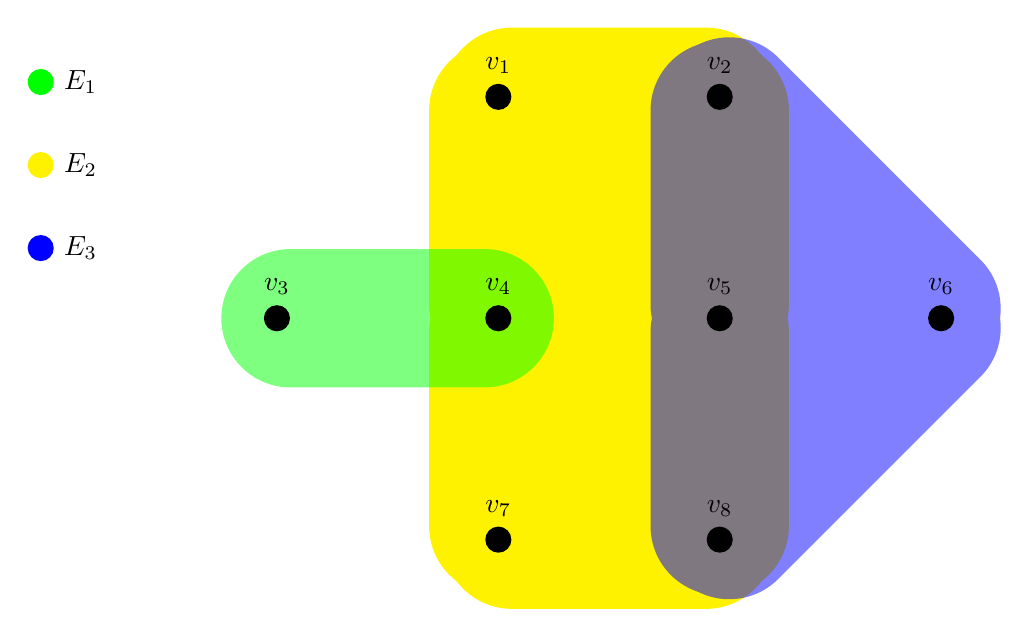
\begin{tikzpicture}
    \tikzstyle{vertex} = [fill,shape=circle,node distance=80pt]
\tikzstyle{edge} = [fill,opacity=.5,fill opacity=.5,line cap=round, line join=round, line width=50pt]
\tikzstyle{edge2} = [fill,opacity=.5,fill opacity=.5,line cap=round, line join=round, line width=30pt]
\tikzstyle{edge3} = [fill,opacity=1,fill opacity=1,line cap=round, line join=round, line width=50pt]

\tikzstyle{elabel} =  [fill,shape=circle,node distance=30pt]

\pgfdeclarelayer{background}
\pgfsetlayers{background,main}

\node[vertex,label=above:\(v_3\)] (v3) {};
\node[vertex,right of=v3,label=above:\(v_4\)] (v4) {};
\node[vertex,above of=v4,label=above:\(v_1\)] (v1) {};
\node[vertex,right of=v4,label=above:\(v_5\)] (v5) {};
\node[vertex,above of=v5,label=above:\(v_2\)] (v2) {};

\node[vertex,right of=v5,label=above:\(v_6\)] (v6) {};
\node[vertex,below of=v4,label=above:\(v_7\)] (v7) {};
\node[vertex,right of=v7,label=above:\(v_8\)] (v8) {};

\begin{pgfonlayer}{background}
\begin{scope}[transparency group,opacity=1]
\draw[edge3,color=yellow] (v1) -- (v2);
\draw[edge3,color=yellow] (v2) -- (v4);

\draw[edge3,color=yellow] (v1) -- (v4);
\draw[edge3,color=yellow] (v4) -- (v7);
\draw[edge3,color=yellow] (v2) -- (v5);
\draw[edge3,color=yellow] (v5) -- (v8);
\draw[edge3,color=yellow] (v5) -- (v7);

\draw[edge3,color=yellow] (v4) -- (v5);
\draw[edge3,color=yellow] (v7) -- (v8);
\end{scope}
\begin{scope}[transparency group,opacity=.5]
\draw[edge,opacity=1,color=green] (v3) -- (v4);
\fill[edge,opacity=1,color=green] (v3.center) -- (v4.center);
\end{scope}
\begin{scope}[transparency group,opacity=.5]
\draw[edge,opacity=1,color=blue] (v5) -- (v6);
\fill[edge,opacity=1,color=blue] (v5.center) -- (v6.center);
\draw[edge,opacity=1,color=blue] (v2) -- (v6);
\fill[edge,opacity=1,color=blue] (v2.center) -- (v6.center);
\draw[edge,opacity=1,color=blue] (v8) -- (v6);
\fill[edge,opacity=1,color=blue] (v8.center) -- (v6.center);
\draw[edge,opacity=1,color=blue] (v2) -- (v5)--(v8);
\fill[edge,opacity=1,color=blue] (v8.center) -- (v6.center);
\end{scope}


\end{pgfonlayer}

\node[elabel,color=green,label=right:\(E_1\)]  (e1) at (-3,3) {};
\node[elabel,below of=e1,color=yellow,label=right:\(E_2\)]  (e2) {};
\node[elabel,below of=e2,color=blue,label=right:\(E_3\)]  (e3) {};
\end{tikzpicture}
\end{center}

  Let $\hgrafeen_2$ be the following hypergraph:
  
  \begin{center}
   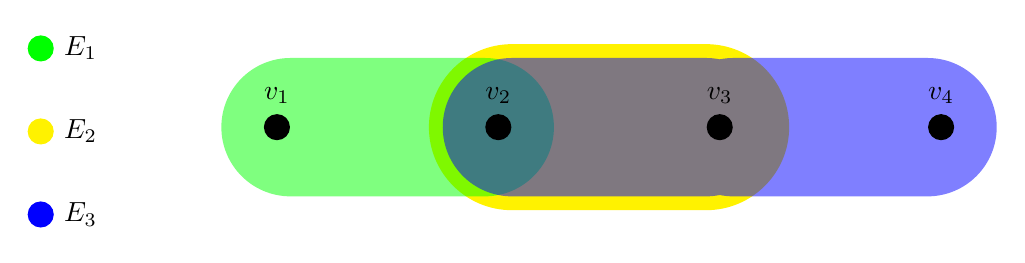
\begin{tikzpicture}
    \tikzstyle{vertex} = [fill,shape=circle,node distance=80pt]
\tikzstyle{edge} = [fill,opacity=.5,fill opacity=.5,line cap=round, line join=round, line width=50pt]
\tikzstyle{edge2} = [fill,opacity=.5,fill opacity=.5,line cap=round, line join=round, line width=30pt]
\tikzstyle{edge3} = [fill,opacity=1,fill opacity=1,line cap=round, line join=round, line width=60pt]

\tikzstyle{elabel} =  [fill,shape=circle,node distance=30pt]

\pgfdeclarelayer{background}
\pgfsetlayers{background,main}

\node[vertex,label=above:\(v_1\)] (v1) {};
\node[vertex,right of=v1,label=above:\(v_2\)] (v2) {};
\node[vertex,right of=v2,label=above:\(v_3\)] (v3) {};
\node[vertex,right of=v3,label=above:\(v_4\)] (v4) {};


\begin{pgfonlayer}{background}
\begin{scope}[transparency group,opacity=1]
\draw[edge3,color=yellow] (v2) -- (v3);

\end{scope}
\begin{scope}[transparency group,opacity=.5]
\draw[edge,opacity=1,color=green] (v1) -- (v2);
\fill[edge,opacity=1,color=green] (v1.center) -- (v2.center);
\end{scope}
\begin{scope}[transparency group,opacity=.5]
\draw[edge,opacity=1,color=blue] (v2)--(v3) -- (v4);
\fill[edge,opacity=1,color=blue] (v3.center) -- (v4.center);
\end{scope}


\end{pgfonlayer}

\node[elabel,color=green,label=right:\(E_1\)]  (e1) at (-3,1) {};
\node[elabel,below of=e1,color=yellow,label=right:\(E_2\)]  (e2) {};
\node[elabel,below of=e2,color=blue,label=right:\(E_3\)]  (e3) {};
\end{tikzpicture}
\end{center}

 And let $\hgrafeen_3$ be the following hypergraph ($\hgrafeen_3$ is in fact also an undirected graph):
  \begin{center}
   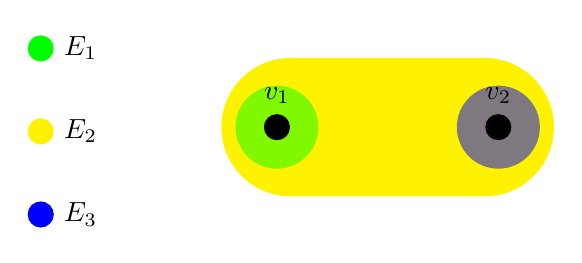
\begin{tikzpicture}
    \tikzstyle{vertex} = [fill,shape=circle,node distance=80pt]
\tikzstyle{edge} = [fill,opacity=.5,fill opacity=.5,line cap=round, line join=round, line width=50pt]
\tikzstyle{edge2} = [fill,opacity=.5,fill opacity=.5,line cap=round, line join=round, line width=30pt]
\tikzstyle{edge3} = [fill,opacity=1,fill opacity=1,line cap=round, line join=round, line width=50pt]

\tikzstyle{elabel} =  [fill,shape=circle,node distance=30pt]

\pgfdeclarelayer{background}
\pgfsetlayers{background,main}

\node[vertex,label=above:\(v_1\)] (v1) {};
\node[vertex,right of=v1,label=above:\(v_2\)] (v2) {};



\begin{pgfonlayer}{background}
\begin{scope}[transparency group,opacity=1]
\draw[edge3,color=yellow] (v1) -- (v2);

\end{scope}
\begin{scope}[transparency group,opacity=.5]
\draw[edge2,opacity=1,color=green] (v1) -- (v1);
\end{scope}
\begin{scope}[transparency group,opacity=.5]
\draw[edge2,opacity=1,color=blue] (v2) -- (v2);
\end{scope}


\end{pgfonlayer}

\node[elabel,color=green,label=right:\(E_1\)]  (e1) at (-3,1) {};
\node[elabel,below of=e1,color=yellow,label=right:\(E_2\)]  (e2) {};
\node[elabel,below of=e2,color=blue,label=right:\(E_3\)]  (e3) {};
\end{tikzpicture}
\end{center}
All off $\hgrafeen_1, \hgrafeen_2$ and $\hgrafeen_3$ lead to the same line-graph 
$\graf$:
\begin{center}
\begin{tikzpicture}[<->,>=stealth',shorten >=1pt,auto,node distance=3cm,
                    thick]
                    \tikzstyle{every node}=[draw,circle,fill=black,minimum size=4pt,
                            inner sep=0pt]


  \node[main node] (1) [label=above:$E_1$] {};
  \node[main node] (2) [label=above:$E_2$][right of=1] {};
  \node[main node] (3) [label=above:$E_3$][right of=2] {};;

  \path[every node/.style={font=\sffamily\small}]
   
    (1) edge node [left] {} (2)
      (2) edge node [left] {} (3)
    
\end{tikzpicture}
\end{center}
\end{example}
\subsubsection{Algorithm for similarity}
We want to apply Algorithm \ref{algsimilarity} to produce a similarity matrix
between two hypergraphs. This will produces an edge similarity matrix, because the vertices are not represented in the line-graph representation. 


To use Algorithm \ref{algsimilarity} from section 2.2, we first take a hypergraph as input and calculate the adjacency matrix of 
the corresponding line-graph. The Matlab implementation of this step can be found in Appendix \ref{appendixa} in Listing \ref{linealgmatlab}. By applying this algorithm to two hypergraphs, we 
can use Algorithm \ref{algsimilarity}. 

\subsubsection{Examples}
We now give some examples of the similarity of two hypergraphs by using 
line-graphs:
\begin{example}\label{ex1line}
  Let $\hgrafeen_1$ be the following hypergraph:
     \begin{center}
   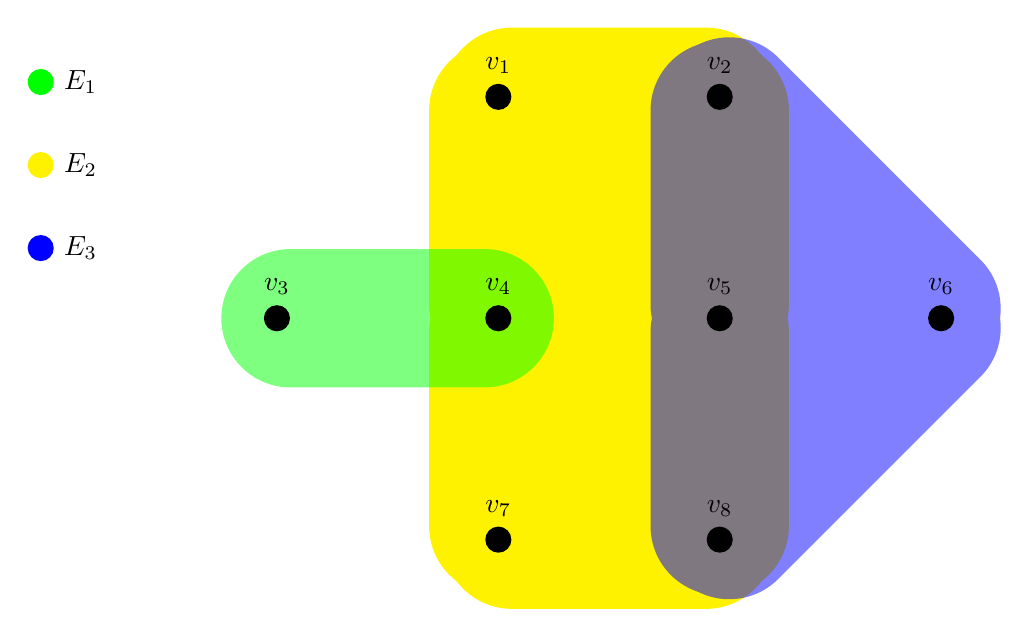
\begin{tikzpicture}
    \tikzstyle{vertex} = [fill,shape=circle,node distance=80pt]
\tikzstyle{edge} = [fill,opacity=.5,fill opacity=.5,line cap=round, line join=round, line width=50pt]
\tikzstyle{edge2} = [fill,opacity=.5,fill opacity=.5,line cap=round, line join=round, line width=30pt]
\tikzstyle{edge3} = [fill,opacity=1,fill opacity=1,line cap=round, line join=round, line width=50pt]

\tikzstyle{elabel} =  [fill,shape=circle,node distance=30pt]

\pgfdeclarelayer{background}
\pgfsetlayers{background,main}

\node[vertex,label=above:\(v_3\)] (v3) {};
\node[vertex,right of=v3,label=above:\(v_4\)] (v4) {};
\node[vertex,above of=v4,label=above:\(v_1\)] (v1) {};
\node[vertex,right of=v4,label=above:\(v_5\)] (v5) {};
\node[vertex,above of=v5,label=above:\(v_2\)] (v2) {};

\node[vertex,right of=v5,label=above:\(v_6\)] (v6) {};
\node[vertex,below of=v4,label=above:\(v_7\)] (v7) {};
\node[vertex,right of=v7,label=above:\(v_8\)] (v8) {};

\begin{pgfonlayer}{background}
\begin{scope}[transparency group,opacity=1]
\draw[edge3,color=yellow] (v1) -- (v2);
\draw[edge3,color=yellow] (v2) -- (v4);

\draw[edge3,color=yellow] (v1) -- (v4);
\draw[edge3,color=yellow] (v4) -- (v7);
\draw[edge3,color=yellow] (v2) -- (v5);
\draw[edge3,color=yellow] (v5) -- (v8);
\draw[edge3,color=yellow] (v5) -- (v7);

\draw[edge3,color=yellow] (v4) -- (v5);
\draw[edge3,color=yellow] (v7) -- (v8);
\end{scope}
\begin{scope}[transparency group,opacity=.5]
\draw[edge,opacity=1,color=green] (v3) -- (v4);
\fill[edge,opacity=1,color=green] (v3.center) -- (v4.center);
\end{scope}
\begin{scope}[transparency group,opacity=.5]
\draw[edge,opacity=1,color=blue] (v5) -- (v6);
\fill[edge,opacity=1,color=blue] (v5.center) -- (v6.center);
\draw[edge,opacity=1,color=blue] (v2) -- (v6);
\fill[edge,opacity=1,color=blue] (v2.center) -- (v6.center);
\draw[edge,opacity=1,color=blue] (v8) -- (v6);
\fill[edge,opacity=1,color=blue] (v8.center) -- (v6.center);
\draw[edge,opacity=1,color=blue] (v2) -- (v5)--(v8);
\fill[edge,opacity=1,color=blue] (v8.center) -- (v6.center);
\end{scope}


\end{pgfonlayer}

\node[elabel,color=green,label=right:\(E_1\)]  (e1) at (-3,3) {};
\node[elabel,below of=e1,color=yellow,label=right:\(E_2\)]  (e2) {};
\node[elabel,below of=e2,color=blue,label=right:\(E_3\)]  (e3) {};
\end{tikzpicture}
\end{center}

  Let $\hgrafeen_2$ be the following hypergraph:
   \begin{center}
   \begin{tikzpicture}
    \tikzstyle{vertex} = [fill,shape=circle,node distance=60pt]
\tikzstyle{edge} = [fill,opacity=.5,fill opacity=.5,line cap=round, line join=round, line width=50pt]
\tikzstyle{edge2} = [fill,opacity=.5,fill opacity=.5,line cap=round, line join=round, line width=30pt]
\tikzstyle{edge3} = [fill,opacity=1,fill opacity=1,line cap=round, line join=round, line width=50pt]

\tikzstyle{elabel} =  [fill,shape=circle,node distance=30pt]

\pgfdeclarelayer{background}
\pgfsetlayers{background,main}

\node[vertex,label=above:\(v_4\)] (v4) {};
\node[vertex,right of=v3,label=above:\(v_5\)] (v5) {};
\node[vertex,right of=v5,label=above:\(v_6\)] (v6) {};

\node[vertex,right of=v6,label=above:\(v_7\)] (v7) {};
\node[vertex,right of=v7,label=above:\(v_8\)] (v8) {};
\node[vertex,right of=v8,label=above:\(v_9\)] (v9) {};
\node[vertex,above of=v6,label=above:\(v_1\)] (v1) {};

\node[vertex,above of=v8,label=above:\(v_3\)] (v3) {};
\node[vertex,above of=v7,label=above:\(v_2\)] (v2) {};


\node[vertex,below of=v6,label=above:\(v_{10}\)] (v10) {};
\node[vertex,right of=v10,label=above:\(v_{11}\)] (v11) {};
\node[vertex,right of=v11,label=above:\(v_{12}\)] (v12) {};


\begin{pgfonlayer}{background}
\begin{scope}[transparency group,opacity=1]
\draw[edge3,color=yellow] (v1) -- (v2);
\draw[edge3,color=yellow] (v2) -- (v7);
\draw[edge3,color=yellow] (v11) -- (v7);
\draw[edge3,color=yellow] (v1) -- (v6);
\draw[edge3,color=yellow] (v1) -- (v7);
\draw[edge3,color=yellow] (v6) -- (v7);
\draw[edge3,color=yellow] (v6) -- (v11);
\draw[edge3,color=yellow] (v6) -- (v10);

\draw[edge3,color=yellow] (v10) -- (v11);

\end{scope}
\begin{scope}[transparency group,opacity=.5]
\draw[edge,opacity=1,color=green] (v4) -- (v5);
\fill[edge,opacity=1,color=green] (v4.center) -- (v5.center);
\end{scope}
\begin{scope}[transparency group,opacity=.5]
\draw[edge,opacity=1,color=blue] (v3) -- (v8);
\fill[edge,opacity=1,color=blue] (v3.center) -- (v8.center);
\draw[edge,opacity=1,color=blue] (v3) -- (v9);
\fill[edge,opacity=1,color=blue] (v3.center) -- (v9.center);
\draw[edge,opacity=1,color=blue] (v9) -- (v8);
\draw[edge,opacity=1,color=blue] (v9) -- (v12);
\fill[edge,opacity=1,color=blue] (v8.center) -- (v6.center);
\draw[edge,opacity=1,color=blue] (v3) -- (v8)--(v12);
\fill[edge,opacity=1,color=blue] (v8.center) -- (v6.center);
\end{scope}
\draw[edge,color=purple] (v5) -- (v6)--(v7)--(v8);


\end{pgfonlayer}

\node[elabel,color=green,label=right:\(E'_1\)]  (e1) at (-3,3) {};
\node[elabel,below of=e1,color=yellow,label=right:\(E'_2\)]  (e2) {};
\node[elabel,below of=e2,color=blue,label=right:\(E'_3\)]  (e3) {};
\node[elabel,below of=e3,color=purple,label=right:\(E'_4\)]  (e4) {};

\end{tikzpicture}
\end{center}

By applying algorithm \ref{linealg} we get the adjacency matrices $A_1$ for 
 $\hgrafeen_1$ and $A_2$ for $\hgrafeen_2$:
 $$A_1 = \begin{pmatrix}
  0 & 1 & 0\\
 1 & 0 & 1\\
  0 & 1 & 0
 \end{pmatrix} \quad \text{and} \quad
 A_2 = \begin{pmatrix}
     0 & 0 & 0 & 1\\
     0 & 0 & 0 & 1\\
     0 & 0 & 0 & 1\\
     1 & 1 & 1 & 0
 \end{pmatrix}
 
 
 Now we use Algorithm \ref{algsimilarity} with $A_1$ and $A_2$ and get the following similarity matrix:
  $$ S = \begin{pmatrix}
      0.2887 &    0.2887  & 0.2887\\
    0.2887  & 0.2887   & 0.2887\\
    0.2887   & 0.2887  & 0.2887\\
    0.2887  &  0.2887  & 0.2887
    \end{pmatrix}$$
    
   \end{example}

\begin{example}\label{ex2line}
  $\hgrafeen_1$ is the same as in the previous example, but now, $\hgrafeen_2$ 
  is the following hypergraph:
   \begin{center}
   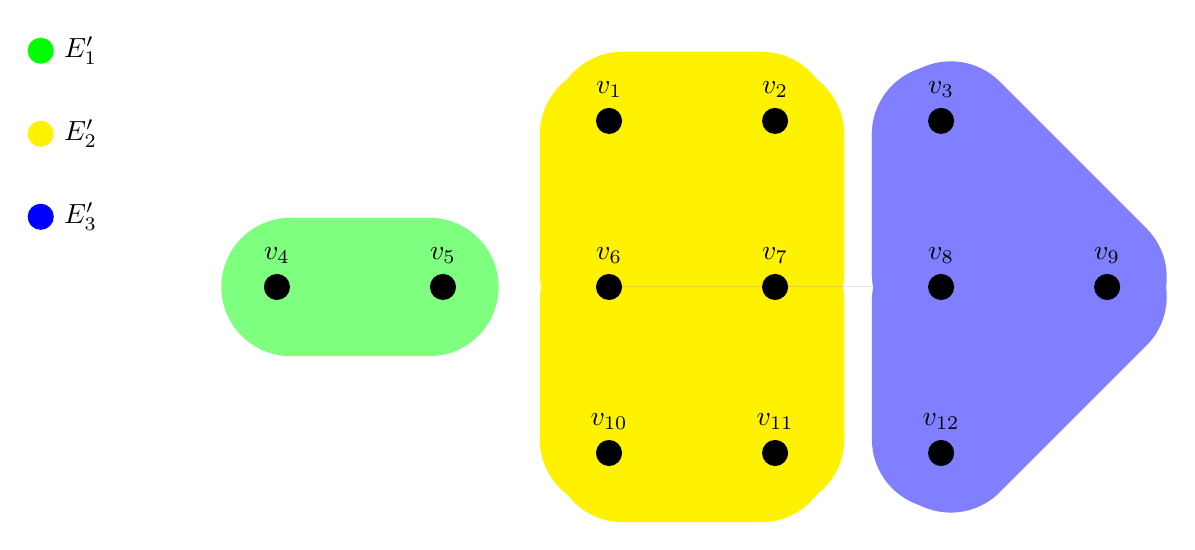
\begin{tikzpicture}
    \tikzstyle{vertex} = [fill,shape=circle,node distance=60pt]
\tikzstyle{edge} = [fill,opacity=.5,fill opacity=.5,line cap=round, line join=round, line width=50pt]
\tikzstyle{edge2} = [fill,opacity=.5,fill opacity=.5,line cap=round, line join=round, line width=30pt]
\tikzstyle{edge3} = [fill,opacity=1,fill opacity=1,line cap=round, line join=round, line width=50pt]

\tikzstyle{elabel} =  [fill,shape=circle,node distance=30pt]

\pgfdeclarelayer{background}
\pgfsetlayers{background,main}

\node[vertex,label=above:\(v_4\)] (v4) {};
\node[vertex,right of=v4,label=above:\(v_5\)] (v5) {};
\node[vertex,right of=v5,label=above:\(v_6\)] (v6) {};

\node[vertex,right of=v6,label=above:\(v_7\)] (v7) {};
\node[vertex,right of=v7,label=above:\(v_8\)] (v8) {};
\node[vertex,right of=v8,label=above:\(v_9\)] (v9) {};
\node[vertex,above of=v6,label=above:\(v_1\)] (v1) {};

\node[vertex,above of=v8,label=above:\(v_3\)] (v3) {};
\node[vertex,above of=v7,label=above:\(v_2\)] (v2) {};


\node[vertex,below of=v6,label=above:\(v_{10}\)] (v10) {};
\node[vertex,right of=v10,label=above:\(v_{11}\)] (v11) {};
\node[vertex,right of=v11,label=above:\(v_{12}\)] (v12) {};


\begin{pgfonlayer}{background}
\begin{scope}[transparency group,opacity=1]
\draw[edge3,color=yellow] (v1) -- (v2);
\draw[edge3,color=yellow] (v2) -- (v7);
\draw[edge3,color=yellow] (v11) -- (v7);
\draw[edge3,color=yellow] (v1) -- (v6);
\draw[edge3,color=yellow] (v1) -- (v7);
\draw[edge3,color=yellow] (v6) -- (v7);
\draw[edge3,color=yellow] (v6) -- (v11);
\draw[edge3,color=yellow] (v6) -- (v10);

\draw[edge3,color=yellow] (v10) -- (v11);

\end{scope}
\begin{scope}[transparency group,opacity=.5]
\draw[edge,opacity=1,color=green] (v4) -- (v5);
\fill[edge,opacity=1,color=green] (v4.center) -- (v5.center);
\end{scope}
\begin{scope}[transparency group,opacity=.5]
\draw[edge,opacity=1,color=blue] (v3) -- (v8);
\fill[edge,opacity=1,color=blue] (v3.center) -- (v8.center);
\draw[edge,opacity=1,color=blue] (v3) -- (v9);
\fill[edge,opacity=1,color=blue] (v3.center) -- (v9.center);
\draw[edge,opacity=1,color=blue] (v9) -- (v8);
\draw[edge,opacity=1,color=blue] (v9) -- (v12);
\fill[edge,opacity=1,color=blue] (v8.center) -- (v6.center);
\draw[edge,opacity=1,color=blue] (v3) -- (v8)--(v12);
\fill[edge,opacity=1,color=blue] (v8.center) -- (v6.center);
\end{scope}


\end{pgfonlayer}

\node[elabel,color=green,label=right:\(E'_1\)]  (e1) at (-3,3) {};
\node[elabel,below of=e1,color=yellow,label=right:\(E'_2\)]  (e2) {};
\node[elabel,below of=e2,color=blue,label=right:\(E'_3\)]  (e3) {};

\end{tikzpicture}
\end{center}
  The similarity score of these two hypergraphs by using their line-graph representation becomes:
  $$S = \begin{pmatrix}
  0 & 0 & 0\\
  0 & 0 & 0\\
  0 & 0 & 0
  \end{pmatrix}$$

\end{example}

\begin{example}\label{ex3line}
  $\hgrafeen_1$ is the same as in the previous example, but now, $\hgrafeen_2$ 
  is the following hypergraph:
   \begin{center}
   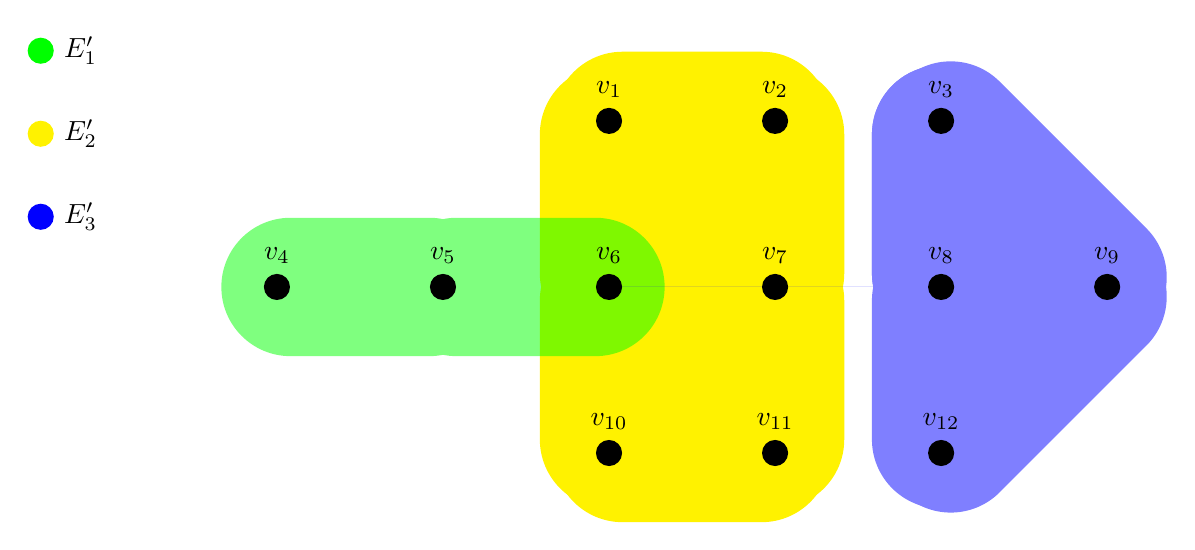
\begin{tikzpicture}
    \tikzstyle{vertex} = [fill,shape=circle,node distance=60pt]
\tikzstyle{edge} = [fill,opacity=.5,fill opacity=.5,line cap=round, line join=round, line width=50pt]
\tikzstyle{edge2} = [fill,opacity=.5,fill opacity=.5,line cap=round, line join=round, line width=30pt]
\tikzstyle{edge3} = [fill,opacity=1,fill opacity=1,line cap=round, line join=round, line width=50pt]

\tikzstyle{elabel} =  [fill,shape=circle,node distance=30pt]

\pgfdeclarelayer{background}
\pgfsetlayers{background,main}

\node[vertex,label=above:\(v_4\)] (v4) {};
\node[vertex,right of=v4,label=above:\(v_5\)] (v5) {};
\node[vertex,right of=v5,label=above:\(v_6\)] (v6) {};

\node[vertex,right of=v6,label=above:\(v_7\)] (v7) {};
\node[vertex,right of=v7,label=above:\(v_8\)] (v8) {};
\node[vertex,right of=v8,label=above:\(v_9\)] (v9) {};
\node[vertex,above of=v6,label=above:\(v_1\)] (v1) {};

\node[vertex,above of=v8,label=above:\(v_3\)] (v3) {};
\node[vertex,above of=v7,label=above:\(v_2\)] (v2) {};


\node[vertex,below of=v6,label=above:\(v_{10}\)] (v10) {};
\node[vertex,right of=v10,label=above:\(v_{11}\)] (v11) {};
\node[vertex,right of=v11,label=above:\(v_{12}\)] (v12) {};


\begin{pgfonlayer}{background}
\begin{scope}[transparency group,opacity=1]
\draw[edge3,color=yellow] (v1) -- (v2);
\draw[edge3,color=yellow] (v2) -- (v7);
\draw[edge3,color=yellow] (v11) -- (v7);
\draw[edge3,color=yellow] (v1) -- (v6);
\draw[edge3,color=yellow] (v1) -- (v7);
\draw[edge3,color=yellow] (v6) -- (v7);
\draw[edge3,color=yellow] (v6) -- (v11);
\draw[edge3,color=yellow] (v6) -- (v10);

\draw[edge3,color=yellow] (v10) -- (v11);

\end{scope}
\begin{scope}[transparency group,opacity=.5]
\draw[edge,opacity=1,color=green] (v4) -- (v5)--(v6);
\fill[edge,opacity=1,color=green] (v4.center) -- (v5.center) -- (v6.center);
\end{scope}
\begin{scope}[transparency group,opacity=.5]
\draw[edge,opacity=1,color=blue] (v3) -- (v8);
\fill[edge,opacity=1,color=blue] (v3.center) -- (v8.center);
\draw[edge,opacity=1,color=blue] (v3) -- (v9);
\fill[edge,opacity=1,color=blue] (v3.center) -- (v9.center);
\draw[edge,opacity=1,color=blue] (v9) -- (v8);
\draw[edge,opacity=1,color=blue] (v9) -- (v12);
\fill[edge,opacity=1,color=blue] (v8.center) -- (v6.center);
\draw[edge,opacity=1,color=blue] (v3) -- (v8)--(v12);
\fill[edge,opacity=1,color=blue] (v8.center) -- (v6.center);
\end{scope}


\end{pgfonlayer}

\node[elabel,color=green,label=right:\(E'_1\)]  (e1) at (-3,3) {};
\node[elabel,below of=e1,color=yellow,label=right:\(E'_2\)]  (e2) {};
\node[elabel,below of=e2,color=blue,label=right:\(E'_3\)]  (e3) {};

\end{tikzpicture}
\end{center}
  The similarity score of these two hypergraphs by using their line-graph representation becomes:
  $$S = \begin{pmatrix}
    0.4082 &    0.4082  &  0.4082\\
    0.4082 &    0.4082  &   0.4082\\
         0      &   0   &      0
  \end{pmatrix}$$

  \end{example}
  
  \begin{example}\label{ex4line}
  $\hgrafeen_1$ is the same as in the previous example, but now, $\hgrafeen_2$ 
  is the following hypergraph:
     \begin{center}
   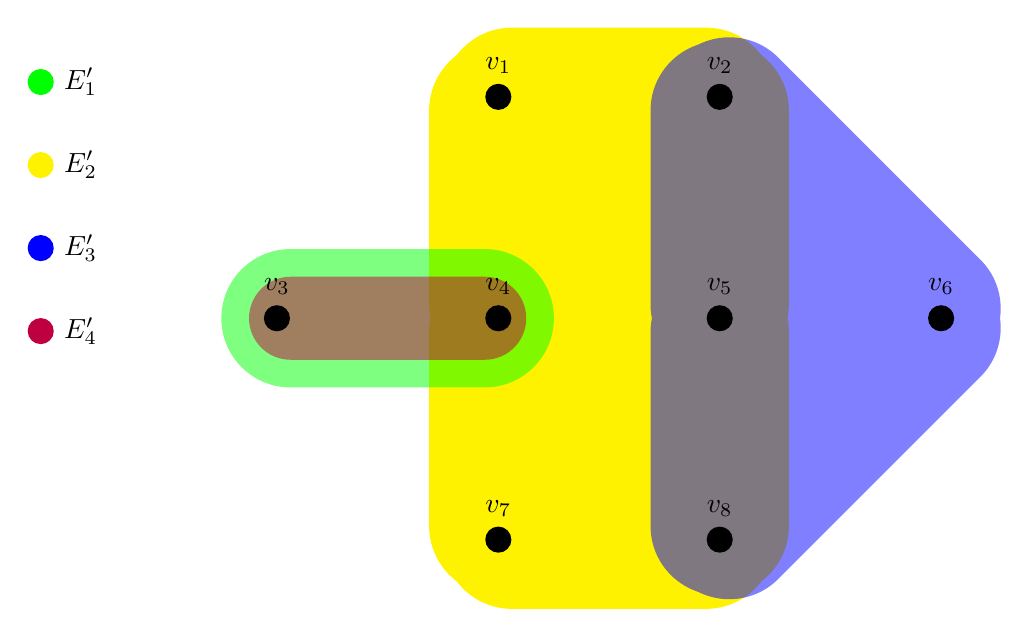
\begin{tikzpicture}
    \tikzstyle{vertex} = [fill,shape=circle,node distance=80pt]
\tikzstyle{edge} = [fill,opacity=.5,fill opacity=.5,line cap=round, line join=round, line width=50pt]
\tikzstyle{edge2} = [fill,opacity=.5,fill opacity=.5,line cap=round, line join=round, line width=30pt]
\tikzstyle{edge3} = [fill,opacity=1,fill opacity=1,line cap=round, line join=round, line width=50pt]

\tikzstyle{elabel} =  [fill,shape=circle,node distance=30pt]

\pgfdeclarelayer{background}
\pgfsetlayers{background,main}

\node[vertex,label=above:\(v_3\)] (v3) {};
\node[vertex,right of=v3,label=above:\(v_4\)] (v4) {};
\node[vertex,above of=v4,label=above:\(v_1\)] (v1) {};
\node[vertex,right of=v4,label=above:\(v_5\)] (v5) {};
\node[vertex,above of=v5,label=above:\(v_2\)] (v2) {};

\node[vertex,right of=v5,label=above:\(v_6\)] (v6) {};
\node[vertex,below of=v4,label=above:\(v_7\)] (v7) {};
\node[vertex,right of=v7,label=above:\(v_8\)] (v8) {};

\begin{pgfonlayer}{background}
\begin{scope}[transparency group,opacity=1]
\draw[edge3,color=yellow] (v1) -- (v2);
\draw[edge3,color=yellow] (v2) -- (v4);

\draw[edge3,color=yellow] (v1) -- (v4);
\draw[edge3,color=yellow] (v4) -- (v7);
\draw[edge3,color=yellow] (v2) -- (v5);
\draw[edge3,color=yellow] (v5) -- (v8);
\draw[edge3,color=yellow] (v5) -- (v7);

\draw[edge3,color=yellow] (v4) -- (v5);
\draw[edge3,color=yellow] (v7) -- (v8);
\end{scope}
\begin{scope}[transparency group,opacity=.5]
\draw[edge,opacity=1,color=green] (v3) -- (v4);
\fill[edge,opacity=1,color=green] (v3.center) -- (v4.center);
\end{scope}
\begin{scope}[transparency group,opacity=.5]
\draw[edge2,opacity=1,color=purple] (v3) -- (v4);
\fill[edge2,opacity=1,color=purple] (v3.center) -- (v4.center);
\end{scope}
\begin{scope}[transparency group,opacity=.5]
\draw[edge,opacity=1,color=blue] (v5) -- (v6);
\fill[edge,opacity=1,color=blue] (v5.center) -- (v6.center);
\draw[edge,opacity=1,color=blue] (v2) -- (v6);
\fill[edge,opacity=1,color=blue] (v2.center) -- (v6.center);
\draw[edge,opacity=1,color=blue] (v8) -- (v6);
\fill[edge,opacity=1,color=blue] (v8.center) -- (v6.center);
\draw[edge,opacity=1,color=blue] (v2) -- (v5)--(v8);
\fill[edge,opacity=1,color=blue] (v8.center) -- (v6.center);
\end{scope}


\end{pgfonlayer}

\node[elabel,color=green,label=right:\(E'_1\)]  (e1) at (-3,3) {};
\node[elabel,below of=e1,color=yellow,label=right:\(E'_2\)]  (e2) {};
\node[elabel,below of=e2,color=blue,label=right:\(E'_3\)]  (e3) {};
\node[elabel,below of=e3,color=purple,label=right:\(E'_4\)]  (e4) {};

\end{tikzpicture}
\end{center}
  The similarity score of these two hypergraphs by using their line-graph representation becomes:
  $$S = \begin{pmatrix}
    0.4082 &    0.4082  & 0 & 0.4082 \\
    0.4082 &    0.4082  &  0&  0.4082 \\
         0      &   0   &      0 & 0
  \end{pmatrix}$$

  \end{example}
  
  \subsubsection{Interpretation}
  We now discuss the conditions from the introduction:
  \begin{itemize}
    \item[(C1)] Not fulfilled: first, the method will only result an edge 
    similarity matrix and second, the line-graph of an undirected graph is not 
    necessary the undirected graph itself:
    \begin{center}
\begin{tikzpicture}[<->,>=stealth',shorten >=1pt,auto,node distance=3cm,
                    thick]
                    \tikzstyle{every node}=[draw,circle,fill=black,minimum size=4pt,
                            inner sep=0pt]


  \node[main node] (1) [label=above:$v_1$] {};
  \node[main node] (2) [label=above:$v_2$][right of=1] {};
  \node[main node] (3) [label=above:$v_3$][right of=2] {};;

  \path[every node/.style={font=\sffamily\small}]
   
    (1) edge node [above] {$e_1$} (2)
      (2) edge node [above] {$e_2$} (3)
    
\end{tikzpicture}
\end{center}
Has as line-graph:

        \begin{center}
\begin{tikzpicture}[<->,>=stealth',shorten >=1pt,auto,node distance=3cm,
                    thick]
                    \tikzstyle{every node}=[draw,circle,fill=black,minimum size=4pt,
                            inner sep=0pt]


  \node[main node] (1) [label=above:$e_1$] {};
  \node[main node] (2) [label=above:$e_2$][right of=1] {};


  \path[every node/.style={font=\sffamily\small}]
   
    (1) edge node [above] {} (2)
    
\end{tikzpicture}
\end{center}
which will clearly not result in the same edge similarity scores as no 
information about the vertex adjacency is saved.
    
    
 
 
   \item[(C2)] Not fulfilled: the vertices of the hypergraph doesn't play a role 
   in the line-graph. No information about them is saved in the line-graph 
   representation.
  \item[(C3)] Fulfilled: Adding an edge to one of the two hypergraphs will 
  result in an extra vertex in the line-graph. Adding this vertex will take the 
  edge into account when calculating the similarity scores and therefore we 
  conclude that this condition is fulfilled.
  \item[(C4)] Not fulfilled: in Examples \ref{ex1line}, \ref{ex2line}, \ref{ex3line}  
  and \ref{ex4line}
  all positive similarity scores are the same, regardless of the adjacency 
  structure of the hypergraph.
  \item[(C5)] Not fulfilled: there is no information about the vertices saved in 
  the line-graph representation of a hypergraph.
  \item[(C6)] Fulfilled: from Example \ref{ex4line} we see that the $E_1$ and 
 $E_4$ are interchangeable and have indeed the same similarity scores.
  \item[(C7)] Not fulfilled: from Example \ref{ex1line} we see that alle edges 
  have exactly the same similarity scores but none of them is interchangeable.
   \item[(C8)] Not fulfilled: no information on the number of vertices an edge 
contains is preserverd by the line-graph representation.
  \item[(C9)] Fulfilled: but it is also the only thing this representation tells us 
  when used for the calculation of similarity: two edges of the two line-graphs
  have a positive similarity score when these edges are connected to other edges, meaning that for any $E_p, E_q$ there is a sequence 
  $$E_p = E_{k_0}, E_{k_1}, \ldots, E_{k_{l-1}}, E_q = E_{k_l}$$
  such that $E_{k_{i-1}} \cap E_{k_i} \not = \emptyset$. From Property 
  \ref{linegrafconnected}, this is not surprising.

  \end{itemize}  
  \subsubsection{Conclusion}
  The line-graph fails to satisfy lots of the conditions and is therefore 
  not a good representation to calculate similarity between two hypergraphs. 
  Similarity between hypergraphs through line-graphs only allows us to discover 
  groups of connected edges in both hypergraphs. The fact that the line-graph 
  representation is a bit disappointing, was also predictable as a lot of 
  hypegraphs share the same line-graph representation. 


\subsection{$2$-section of a hypergraph}
\subsubsection{General definitions and properties}
We now look at another graph representation of a hypergraph. In contrast to the 
line-graph representation, the $2$-section saves information about the vertices 
which will introduce a more sophisticated way to say something about 
similarity between two hypergraphs by using their $2$-section.

\begin{defintion}
  The \textbf{$2$-section} of a hypergraph $\hgrafeen = (V,E)$ is the (undirected) graph denoted by $\[\hgrafeen\]_2 = (V,\to)$ 
  with:
  \begin{itemize}
    \item The same vertex set as the hypergraph,
    \item $v_i \to v_j$ if and only if $v_i, v_j \in E_k$ for some $E_k \in E$ and $i \not = j$.
  \end{itemize}
  \end{defintion}
  
\begin{example}\label{uniciteitsvoorbeeld}
The 2-section of the following hypergraph $\hgrafeen$ is drawn on top:
    \begin{center}
   \begin{tikzpicture}
    \tikzstyle{vertex} = [fill,shape=circle,node distance=80pt]
\tikzstyle{edge} = [fill,opacity=.5,fill opacity=.5,line cap=round, line join=round, line width=50pt]
\tikzstyle{edge2} = [fill,opacity=.5,fill opacity=.5,line cap=round, line join=round, line width=30pt]
\tikzstyle{edge3} = [fill,opacity=1,fill opacity=1,line cap=round, line join=round, line width=50pt]
\tikzstyle{gedge} = [<->,>=stealth',shorten >=1pt, auto,node distance=3cm,
                    thick]
                    \tikzstyle{gedge30} = [<->,>=stealth',shorten >=1pt,bend right=30, auto,node distance=3cm,
                    thick]
\tikzstyle{elabel} =  [fill,shape=circle,node distance=30pt]

\pgfdeclarelayer{background}
\pgfsetlayers{background,main}

\node[vertex,label=above:\(v_3\)] (v3) {};
\node[vertex,right of=v3,label=above left:\(v_4\)] (v4) {};
\node[vertex,above of=v4,label=above:\(v_1\)] (v1) {};
\node[vertex,right of=v4,label=above right:\(v_5\)] (v5) {};
\node[vertex,above of=v5,label=above:\(v_2\)] (v2) {};

\node[vertex,right of=v5,label=above:\(v_6\)] (v6) {};
\node[vertex,below of=v4,label=below:\(v_7\)] (v7) {};
\node[vertex,right of=v7,label=below:\(v_8\)] (v8) {};



\begin{pgfonlayer}{background}
\begin{scope}[transparency group,opacity=1]
\draw[edge3,color=yellow] (v1) -- (v2);
\draw[edge3,color=yellow] (v2) -- (v4);

\draw[edge3,color=yellow] (v1) -- (v4);
\draw[edge3,color=yellow] (v4) -- (v7);
\draw[edge3,color=yellow] (v2) -- (v5);
\draw[edge3,color=yellow] (v5) -- (v8);
\draw[edge3,color=yellow] (v5) -- (v7);

\draw[edge3,color=yellow] (v4) -- (v5);
\draw[edge3,color=yellow] (v7) -- (v8);
\end{scope}
\begin{scope}[transparency group,opacity=.5]
\draw[edge,opacity=1,color=green] (v3) -- (v4);
\fill[edge,opacity=1,color=green] (v3.center) -- (v4.center);
\end{scope}
\begin{scope}[transparency group,opacity=.5]
\draw[edge,opacity=1,color=blue] (v5) -- (v6);
\fill[edge,opacity=1,color=blue] (v5.center) -- (v6.center);
\draw[edge,opacity=1,color=blue] (v2) -- (v6);
\fill[edge,opacity=1,color=blue] (v2.center) -- (v6.center);
\draw[edge,opacity=1,color=blue] (v8) -- (v6);
\fill[edge,opacity=1,color=blue] (v8.center) -- (v6.center);
\draw[edge,opacity=1,color=blue] (v2) -- (v5)--(v8);
\fill[edge,opacity=1,color=blue] (v8.center) -- (v6.center);
\end{scope}
\begin{scope}[transparency group,opacity=1]
  \draw[gedge,opacity=1,color=black] (v3) -- (v4);
  \draw[gedge,opacity=1,color=black] (v1) -- (v4);
  \draw[gedge,opacity=1,color=black] (v2) -- (v4);
   \draw[gedge,opacity=1,color=black] (v5) -- (v4);
  \draw[gedge,opacity=1,color=black] (v8) -- (v4);
  \draw[gedge,opacity=1,color=black] (v7) -- (v4);
   \draw[gedge,opacity=1,color=black] (v1) -- (v2);
  \draw[gedge,opacity=1,color=black] (v1) -- (v5);
  \draw[gedge,opacity=1,color=black] (v1) -- (v8);
   \draw[gedge30, bent left=100, opacity=1,color=black] (v1) -- (v7);
  \draw[gedge,opacity=1,color=black] (v2) -- (v5);
  \draw[gedge,opacity=1,color=black] (v2) -- (v8);
   \draw[gedge,opacity=1,color=black] (v2) -- (v7);
  \draw[gedge,opacity=1,color=black] (v2) -- (v6);
  \draw[gedge,opacity=1,color=black] (v5) -- (v7);
    \draw[gedge,opacity=1,color=black] (v5) -- (v8);
    \draw[gedge,opacity=1,color=black] (v5) -- (v6);
      \draw[gedge,opacity=1,color=black] (v8) -- (v6);
      \end{scope}
      \begin{scope}[transparency group,opacity=1]

      \draw[gedge30, opacity=1, bend left] (v1) -- (v7);
\end{scope}

\end{pgfonlayer}

\node[elabel,color=green,label=right:\(E_1\)]  (e1) at (-3,3) {};
\node[elabel,below of=e1,color=yellow,label=right:\(E_2\)]  (e2) {};
\node[elabel,below of=e2,color=blue,label=right:\(E_3\)]  (e3) {};
\end{tikzpicture}
\end{center}
\end{example}

Also the 2-section of a hypergraph is not a faithful graph characteristic of a hypergraph, as the following example 
shows:

\begin{example}\label{2sectievoorbeeld}
The 2-section of the following hypergraph $\hgrafeen'$ is drawn on top and is the same as the previous example:

      \begin{center}
   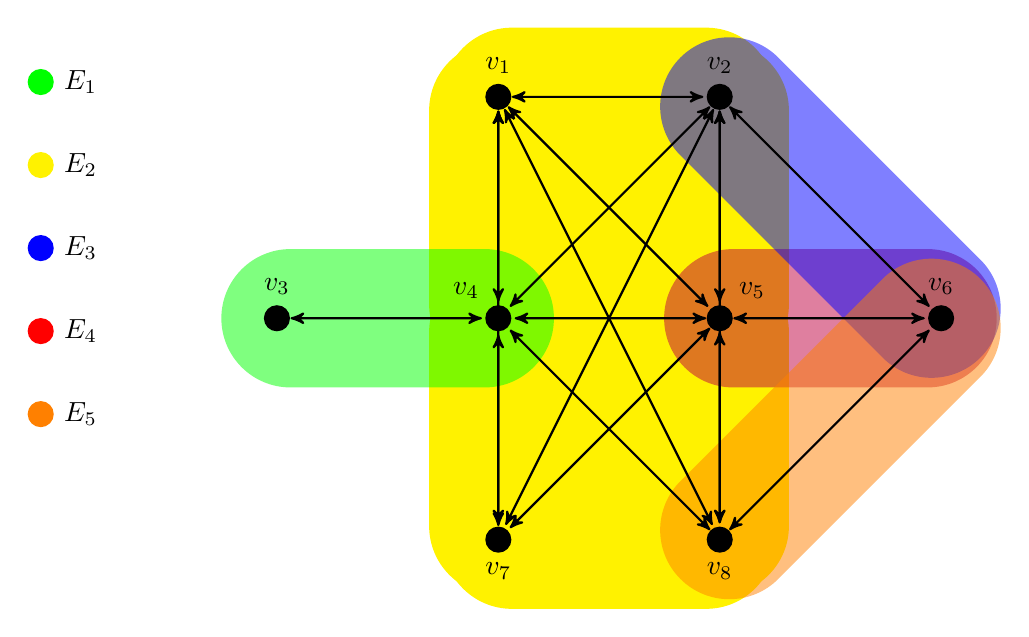
\begin{tikzpicture}
    \tikzstyle{vertex} = [fill,shape=circle,node distance=80pt]
\tikzstyle{edge} = [fill,opacity=.5,fill opacity=.5,line cap=round, line join=round, line width=50pt]
\tikzstyle{edge2} = [fill,opacity=.5,fill opacity=.5,line cap=round, line join=round, line width=30pt]
\tikzstyle{edge3} = [fill,opacity=1,fill opacity=1,line cap=round, line join=round, line width=50pt]
\tikzstyle{gedge} = [<->,>=stealth',shorten >=1pt, auto,node distance=3cm,
                    thick]
                    \tikzstyle{gedge30} = [<->,>=stealth',shorten >=1pt,bend right=30, auto,node distance=3cm,
                    thick]
\tikzstyle{elabel} =  [fill,shape=circle,node distance=30pt]

\pgfdeclarelayer{background}
\pgfsetlayers{background,main}

\node[vertex,label=above:\(v_3\)] (v3) {};
\node[vertex,right of=v3,label=above left:\(v_4\)] (v4) {};
\node[vertex,above of=v4,label=above:\(v_1\)] (v1) {};
\node[vertex,right of=v4,label=above right:\(v_5\)] (v5) {};
\node[vertex,above of=v5,label=above:\(v_2\)] (v2) {};

\node[vertex,right of=v5,label=above:\(v_6\)] (v6) {};
\node[vertex,below of=v4,label=below:\(v_7\)] (v7) {};
\node[vertex,right of=v7,label=below:\(v_8\)] (v8) {};



\begin{pgfonlayer}{background}
\begin{scope}[transparency group,opacity=1]
\draw[edge3,color=yellow] (v1) -- (v2);
\draw[edge3,color=yellow] (v2) -- (v4);

\draw[edge3,color=yellow] (v1) -- (v4);
\draw[edge3,color=yellow] (v4) -- (v7);
\draw[edge3,color=yellow] (v2) -- (v5);
\draw[edge3,color=yellow] (v5) -- (v8);
\draw[edge3,color=yellow] (v5) -- (v7);

\draw[edge3,color=yellow] (v4) -- (v5);
\draw[edge3,color=yellow] (v7) -- (v8);
\end{scope}
\begin{scope}[transparency group,opacity=.5]
\draw[edge,opacity=1,color=green] (v3) -- (v4);
\fill[edge,opacity=1,color=green] (v3.center) -- (v4.center);
\end{scope}
\begin{scope}[transparency group,opacity=.5]
\draw[edge,opacity=1,color=purple] (v5) -- (v6);
\fill[edge,opacity=1,color=purple] (v5.center) -- (v6.center);
\end{scope}
\begin{scope}[transparency group,opacity=.5]

\draw[edge,opacity=1,color=blue] (v2) -- (v6);
\fill[edge,opacity=1,color=blue] (v2.center) -- (v6.center);
\end{scope}
\begin{scope}[transparency group,opacity=.5]

\draw[edge,opacity=1,color=orange] (v8) -- (v6);
\fill[edge,opacity=1,color=orange] (v8.center) -- (v6.center);

\end{scope}
\begin{scope}[transparency group,opacity=1]
  \draw[gedge,opacity=1,color=black] (v3) -- (v4);
  \draw[gedge,opacity=1,color=black] (v1) -- (v4);
  \draw[gedge,opacity=1,color=black] (v2) -- (v4);
   \draw[gedge,opacity=1,color=black] (v5) -- (v4);
  \draw[gedge,opacity=1,color=black] (v8) -- (v4);
  \draw[gedge,opacity=1,color=black] (v7) -- (v4);
   \draw[gedge,opacity=1,color=black] (v1) -- (v2);
  \draw[gedge,opacity=1,color=black] (v1) -- (v5);
  \draw[gedge,opacity=1,color=black] (v1) -- (v8);
   \draw[gedge30, bend right=100, opacity=1,color=black] (v1) -- (v7);
  \draw[gedge,opacity=1,color=black] (v2) -- (v5);
  \draw[gedge,opacity=1,color=black] (v2) -- (v8);
   \draw[gedge,opacity=1,color=black] (v2) -- (v7);
  \draw[gedge,opacity=1,color=black] (v2) -- (v6);
  \draw[gedge,opacity=1,color=black] (v5) -- (v7);
    \draw[gedge,opacity=1,color=black] (v5) -- (v8);
    \draw[gedge,opacity=1,color=black] (v5) -- (v6);
      \draw[gedge,opacity=1,color=black] (v8) -- (v6);
\end{scope}

\end{pgfonlayer}

\node[elabel,color=green,label=right:\(E_1\)]  (e1) at (-3,3) {};
\node[elabel,below of=e1,color=yellow,label=right:\(E_2\)]  (e2) {};
\node[elabel,below of=e2,color=blue,label=right:\(E_3\)]  (e3) {};
\node[elabel,below of=e3,color=red,label=right:\(E_4\)]  (e4) {};
\node[elabel,below of=e4,color=orange,label=right:\(E_5\)]  (e5) {};
\end{tikzpicture}
\end{center}
\end{example}
\subsubsection{Algorithm for similarity}
  In Listing \ref{2sectionalgmatlab} in Appenix \ref{appendixa}, we introduce 
  an algorithm that 
  takes a hypergraph as input and returns the adjacency matrix of the 
  corresponding $2$-section of the hypergraph. The 
  resulting adjacency matrix can then be used in the node similarity method from 
  Algorithm \ref{algsimilarity}.
  
  
  
\subsubsection{Examples}
We now use the same examples as in the previous subsection and look at what the 
similarity of two hypergraphs becomes by using their $2$-section.
\begin{example}\label{ex2sec1}
  Take the same $\hgrafeen_1$ and $\hgrafeen_2$ as in Example \ref{ex1line}, 
by calculating the adjacency matrices of the 2-section,
   and we can apply Algorithm \ref{algsimilarity}  which returns the similarity 
   matrix:
   $$ S = \begin{pmatrix}
0.1347&0.1479&0.0261&0.1388&0.1479&0.0833&0.1347&0.1479\\
0.1347&0.1479&0.0261&0.1388&0.1479&0.0833&0.1347&0.1479\\
0.0263&0.0288&0.0051&0.0271&0.0288&0.0162&0.0263&0.0288\\
0.0147&0.0161&0.0028&0.0151&0.0161&0.0091&0.0147&0.0161\\
0.0790&0.0867&0.0153&0.0814&0.0867&0.0489&0.0790&0.0867\\
0.1610&0.1768&0.0312&0.1659&0.1768&0.0996&0.1610&0.1768\\
0.1610&0.1768&0.0312&0.1659&0.1768&0.0996&0.1610&0.1768\\
0.0890&0.0977&0.0172&0.0917&0.0977&0.0551&0.0890&0.0977\\
0.0263&0.0288&0.0051&0.0271&0.0288&0.0162&0.0263&0.0288\\
0.1347&0.1479&0.0261&0.1388&0.1479&0.0833&0.1347&0.1479\\
0.1347&0.1479&0.0261&0.1388&0.1479&0.0833&0.1347&0.1479\\
0.0263&0.0288&0.0051&0.0271&0.0288&0.0162&0.0263&0.0288
\end{pmatrix} $$


 \end{example}

 \begin{example}\label{ex2sec2}
   Let $\hgrafeen_1$ and $\hgrafeen_2$ be the same as in Example \ref{ex2line}, 
   the similarity matrix using the 2-section of the hypergraphs becomes:
   $$S = \begin{pmatrix}
   0.1532&0.1682&0.0297&0.1579&0.1682&0.0948&0.1532&0.1682\\
0.1532&0.1682&0.0297&0.1579&0.1682&0.0948&0.1532&0.1682\\
0&0&0&0&0&0&0&0\\
0&0&0&0&0&0&0&0\\
0&0&0&0&0&0&0&0\\
0.1532&0.1682&0.0297&0.1579&0.1682&0.0948&0.1532&0.1682\\
0.1532&0.1682&0.0297&0.1579&0.1682&0.0948&0.1532&0.1682\\
0&0&0&0&0&0&0&0\\
0&0&0&0&0&0&0&0\\
0.1532&0.1682&0.0297&0.1579&0.1682&0.0948&0.1532&0.1682\\
0.1532&0.1682&0.0297&0.1579&0.1682&0.0948&0.1532&0.1682\\
0&0&0&0&0&0&0&0
   \end{pmatrix}$$
   \end{example}
 
\begin{example}\label{ex2sec3}
     Let $\hgrafeen_1$ and $\hgrafeen_2$ be the same as in Example \ref{ex3line}, 
   the similarity matrix using the 2-section of the hypergraphs becomes:
   $$S = \begin{pmatrix}
0.1493&0.1639&0.0289&0.1538&0.1639&0.0923&0.1493&0.1639\\
0.1493&0.1639&0.0289&0.1538&0.1639&0.0923&0.1493&0.1639\\
0&0&0&0&0&0&0&0\\
0.0397&0.0436&0.0077&0.0409&0.0436&0.0246&0.0397&0.0436\\
0.0397&0.0436&0.0077&0.0409&0.0436&0.0246&0.0397&0.0436\\
0.1623&0.1782&0.0314&0.1673&0.1782&0.1004&0.1623&0.1782\\
0.1493&0.1639&0.0289&0.1538&0.1639&0.0923&0.1493&0.1639\\
0&0&0&0&0&0&0&0\\
0&0&0&0&0&0&0&0\\
0.1493&0.1639&0.0289&0.1538&0.1639&0.0923&0.1493&0.1639\\
0.1493&0.1639&0.0289&0.1538&0.1639&0.0923&0.1493&0.1639\\
0&0&0&0&0&0&0&0
   \end{pmatrix}$$
   
\end{example}
\subsubsection{Interpretation}

\begin{itemize}
  \item[(C1)] Not fulfilled: an undirected graph with multiple edges between two vertices $v_p, v_q$ will `lose' this
  edges in its 2-section. Also loops are not taken into consideration. Take for example the following graph $\graf$:
   \begin{center}
\begin{tikzpicture}[<->,>=stealth',shorten >=1pt,auto,node distance=3cm,
                    thick]
                    \tikzstyle{every node}=[draw,circle,fill=black,minimum size=4pt,
                            inner sep=0pt]


  \node[main node] (1) [label=above:$v_1$] {};
  \node[main node] (2) [label=above:$v_2$][right of=1] {};

  \path[every node/.style={font=\sffamily\small}]
   
    (1) edge node [above] {$e_1$} (2)
      (1) edge[bend left=30] node [above] {$e_2$} (2)
           (1) edge [loop below] node {$e_3$} (1)

    
\end{tikzpicture}

\end{center} 
$\graf$ will have as 2-section:
 \begin{center}
\begin{tikzpicture}[<->,>=stealth',shorten >=1pt,auto,node distance=3cm,
                    thick]
                    \tikzstyle{every node}=[draw,circle,fill=black,minimum size=4pt,
                            inner sep=0pt]


  \node[main node] (1) [label=above:$v_1$] {};
  \node[main node] (2) [label=above:$v_2$][right of=1] {};

  \path[every node/.style={font=\sffamily\small}]
   
    (1) edge node [above] {$e_1$} (2)
      
    
\end{tikzpicture}

\end{center}
  \item[(C2)] Fulfilled: the number of vertices is preserved in the 2-section of 
  a hypergraph.
  \item[(C3)] Not fulfilled: introducing an edge in a hypergraph that connects vertices who are already connected, 
doesn't change anything to the 2-section of the hypergraph (by definition), for 
instance if we take $\hgrafeen_1$ in Example \ref{ex2sec1} as follows:
   \begin{center}
   \begin{tikzpicture}
    \tikzstyle{vertex} = [fill,shape=circle,node distance=80pt]
\tikzstyle{edge} = [fill,opacity=.5,fill opacity=.5,line cap=round, line join=round, line width=50pt]
\tikzstyle{edge2} = [fill,opacity=.5,fill opacity=.5,line cap=round, line join=round, line width=40pt]
\tikzstyle{edge3} = [fill,opacity=1,fill opacity=1,line cap=round, line join=round, line width=50pt]

\tikzstyle{elabel} =  [fill,shape=circle,node distance=30pt]

\pgfdeclarelayer{background}
\pgfsetlayers{background,main}

\node[vertex,label=above:\(v_3\)] (v3) {};
\node[vertex,right of=v3,label=above:\(v_4\)] (v4) {};
\node[vertex,above of=v4,label=above:\(v_1\)] (v1) {};
\node[vertex,right of=v4,label=above:\(v_5\)] (v5) {};
\node[vertex,above of=v5,label=above:\(v_2\)] (v2) {};

\node[vertex,right of=v5,label=above:\(v_6\)] (v6) {};
\node[vertex,below of=v4,label=above:\(v_7\)] (v7) {};
\node[vertex,right of=v7,label=above:\(v_8\)] (v8) {};

\begin{pgfonlayer}{background}
\begin{scope}[transparency group,opacity=1]
\draw[edge3,color=yellow] (v1) -- (v2);
\draw[edge3,color=yellow] (v2) -- (v4);

\draw[edge3,color=yellow] (v1) -- (v4);
\draw[edge3,color=yellow] (v4) -- (v7);
\draw[edge3,color=yellow] (v2) -- (v5);
\draw[edge3,color=yellow] (v5) -- (v8);
\draw[edge3,color=yellow] (v5) -- (v7);

\draw[edge3,color=yellow] (v4) -- (v5);
\draw[edge3,color=yellow] (v7) -- (v8);
\end{scope}
\begin{scope}[transparency group,opacity=.5]
\draw[edge,opacity=1,color=green] (v3) -- (v4);
\fill[edge,opacity=1,color=green] (v3.center) -- (v4.center);
\end{scope}
\begin{scope}[transparency group,opacity=.5]
\draw[edge,opacity=1,color=blue] (v5) -- (v6);
\fill[edge,opacity=1,color=blue] (v5.center) -- (v6.center);
\draw[edge,opacity=1,color=blue] (v2) -- (v6);
\fill[edge,opacity=1,color=blue] (v2.center) -- (v6.center);
\draw[edge,opacity=1,color=blue] (v8) -- (v6);
\fill[edge,opacity=1,color=blue] (v8.center) -- (v6.center);
\draw[edge,opacity=1,color=blue] (v2) -- (v5)--(v8);
\fill[edge,opacity=1,color=blue] (v8.center) -- (v6.center);
\draw[edge2,opacity=0.7,color=purple] (v1) -- (v4);
\end{scope}


\end{pgfonlayer}

\node[elabel,color=green,label=right:\(E_1\)]  (e1) at (-3,3) {};
\node[elabel,below of=e1,color=yellow,label=right:\(E_2\)]  (e2) {};
\node[elabel,below of=e2,color=blue,label=right:\(E_3\)]  (e3) {};
\node[elabel,below of=e4,color=purple,label=right:\(E_4\)]  (e4) {};

\end{tikzpicture}
\end{center}
then we will get the same similarity matrix as the introduced edge $E_4$ will not influence the similarity scores at all 
because $v_1, v_4, v_7$ were already adjacent to each other in the 2-section of 
$\hgrafeen_1$. 

  \item[(C4)] Fulfilled: take for Example \ref{ex2sec1}, we see that the largest similarity scores
  occurs between vertices $v_6, v_7$ 
  in $\hgrafeen_2$ and vertices $v_2, v_5$ and $v_8$ from $\hgrafeen_1$. This can 
  be explained by the fact that indeed $v_6,v_7$ are all adjacent to the vertices in $E_2$. And that $E_2$ is the 
  most central set of vertices in the whole hypergraph. 
  
  This can be explained 
  generally by the fact that the 2-section preserves the adjacency relations between 
  vertices of the hypergraph by definition. Therefore, this is a consequence 
  from Algorithm \ref{algsimilarity} that returns a high similarity score of a 
  vertex in a graph (in this case the 2-section of the hypergraph) when the similarity score of the adjacent vertices is large.
    \item[(C5)] This condition does not apply on this method because we don't calculate edge similarity scores.
   \item[(C6)] Fulfilled: all interchangeable vertices have the same similarity 
   scores in the Examples \ref{ex2sec1}, \ref{ex2sec2}, \ref{ex2sec3}. This is can be explained
   by the fact that the interchangeable vertices of a hypergraph are also 
   interchangeable vertices in the 2-section graph.
   
   
     \item[(C7)] Not fulfilled: we know from (C3) that edges that connect 
     vertices that where already connected by other edges have no effect on
   the 2-section. This means that $\hgrafeen$ in the example in (C3) would 
     return the same similarity scores for $v_1$ and $v_7$ although they are not 
     interchangeable.
     \item [(C8)] Not fulfilled: the $2$-section doesn't save any information 
     about the number of vertices in each edge. 
  \item[(C9)] Fulfilled by the fact that isolated vertices in a hypergraph will 
  also be isolated in the 2-section.
  \end{itemize}  

\subsubsection{Conclusion}
The $2$-section of a hypergraph is a rich structure that 
saves a lot more information compared to the the line-graph representation. The biggest drawback for this method is that 
adding an edge to a hypergraph can sometimes have no effect at all. This happens when 
the added edge connects vertices which were already connected. This is bad, because adding an edge always should have an impact on 
  the similarity scores as it expresses a union between vertices. As a consequence, adjacent vertices that aren't interchangeable
  can still have the same similarity scores. We saw in Example \ref{2sectievoorbeeld} that
  the 2-section of a hypergraph is not unique, meaning that we are loosing certain
  information on the hypergraph. In this case, we can lose information about 
  the edges as some edges will not be represented in the 2 section and we also lose 
  all information about 
  the number of vertices contained in each edge. Meaning that the number of vertices
  contained in an edge doesn't play any role when calculating the similarity scores. 
  
 We can resolve the problems in conditions (C1), (C3) and (C7) by allowing multiple edges
  between vertices and loops: every edge in the hypergraph is then also represented in this \emph{extended 2-section}.
  
  \subsection{Extended $2$-section of a hypergraph}
 \subsubsection{General definitions and properties}
\begin{defintion}
  The \textbf{extended $2$-section} of a hypergraph $\hgrafeen = (V,E)$ is the (undirected) graph denoted by $\[\hgrafeen\]'_2 = (V,\to)$ 
  with:
  \begin{itemize}
    \item The same vertex set as the hypergraph,
    \item for every $E_i \in E$ with $|E_i| > 1$: $v_k \to v_l$ for every $v_k, v_l \in E_i and k \not 
    = l$,
    \item for every $E_i \in E$ with $|E_i| =1$ : $v_k \to v_k$ for $v_k \in 
    E_i$.
    \end{itemize}
      \end{defintion}
\subsubsection{Algorithm for similarity}
We introduce Algorithm \ref{extended2sectionalg} that 
  takes a hypergraph as input and returns the adjacency matrix of the 
  corresponding  extended $2$-section of the hypergraph. A Matlab implementation can be 
  found in Listing \ref{extended2sectionalgmatlab} in Appenix \ref{appendixa}.
  
  
  \begin{algorithm}[H]\label{extended2sectionalg}
 \KwData{\\
 $n$:  the number of vertices of hypergraph $\hgrafeen$\\
 $E$:  a set of subsets $E_i$ of $\{1, \ldots, n\}$ that represent the edges of hypergraph $\hgrafeen$\\
 \KwResult{\\
 $A$: the adjacency matrix of the corresponding extended 2-section}
 \blankline
\SetKwFunction{powermethod}{hypergraph\_to\_extended2section}
\SetKwFunction{hits}{hits}

\SetKwProg{myalg}{begin}{}{end}
\myalg{\powermethod{$n$, $E$}}{
$A$ = initialize a $n \times n$-matrix with all entries equal to 0\;
$m$ = number of edges\;
\For{$i: 1$ to $m$ }{
      \eIf{$|E_m|$ = 1}{
         $k =$ vertex in $E_m$\;
         $(A)_{kk} = A_{kk} + 1$\;
     }{
     \For{$j: 1$ to $|E_m|$}{
     $C = $ all possible combinations of elements in $E_m \backslash j$\;
       \For{$l: 1$ to $|C|$}{
       $A_{jl} = A_{jl} + 1$
       } 
     }
     
          }
  }}
\KwRet $A$\;}{}
  \caption{Algorithm to calculate the adjacency matrix of the extended 2-section of a hypergraph.\\}
\end{algorithm}


\subsubsection{Example}
We take an example that really shows the power of 
extended 2-sections:
\begin{example}
  Take $\hgrafeen_1$ as in Example \ref{ex1line} and $\hgrafeen_2$:
  \begin{center}
   \begin{tikzpicture}
    \tikzstyle{vertex} = [fill,shape=circle,node distance=80pt]
\tikzstyle{edge} = [fill,opacity=.5,fill opacity=.5,line cap=round, line join=round, line width=50pt]
\tikzstyle{edge2} = [fill,opacity=.5,fill opacity=.5,line cap=round, line join=round, line width=40pt]
\tikzstyle{edge3} = [fill,opacity=1,fill opacity=1,line cap=round, line join=round, line width=50pt]

\tikzstyle{elabel} =  [fill,shape=circle,node distance=30pt]

\pgfdeclarelayer{background}
\pgfsetlayers{background,main}

\node[vertex,label=above:\(v_3\)] (v3) {};
\node[vertex,right of=v3,label=above:\(v_4\)] (v4) {};
\node[vertex,above of=v4,label=above:\(v_1\)] (v1) {};
\node[vertex,right of=v4,label=above:\(v_5\)] (v5) {};
\node[vertex,above of=v5,label=above:\(v_2\)] (v2) {};

\node[vertex,right of=v5,label=above:\(v_6\)] (v6) {};
\node[vertex,below of=v4,label=above:\(v_7\)] (v7) {};
\node[vertex,right of=v7,label=above:\(v_8\)] (v8) {};

\begin{pgfonlayer}{background}
\begin{scope}[transparency group,opacity=1]
\draw[edge3,color=yellow] (v1) -- (v2);
\draw[edge3,color=yellow] (v2) -- (v4);

\draw[edge3,color=yellow] (v1) -- (v4);
\draw[edge3,color=yellow] (v4) -- (v7);
\draw[edge3,color=yellow] (v2) -- (v5);
\draw[edge3,color=yellow] (v5) -- (v8);
\draw[edge3,color=yellow] (v5) -- (v7);

\draw[edge3,color=yellow] (v4) -- (v5);
\draw[edge3,color=yellow] (v7) -- (v8);
\end{scope}
\begin{scope}[transparency group,opacity=.5]
\draw[edge,opacity=1,color=green] (v3) -- (v4);
\fill[edge,opacity=1,color=green] (v3.center) -- (v4.center);
\end{scope}
\begin{scope}[transparency group,opacity=.5]
\draw[edge,opacity=1,color=blue] (v5) -- (v6);
\fill[edge,opacity=1,color=blue] (v5.center) -- (v6.center);
\draw[edge,opacity=1,color=blue] (v2) -- (v6);
\fill[edge,opacity=1,color=blue] (v2.center) -- (v6.center);
\draw[edge,opacity=1,color=blue] (v8) -- (v6);
\fill[edge,opacity=1,color=blue] (v8.center) -- (v6.center);
\draw[edge,opacity=1,color=blue] (v2) -- (v5)--(v8);
\fill[edge,opacity=1,color=blue] (v8.center) -- (v6.center);
\draw[edge2,opacity=0.7,color=purple] (v1) -- (v4);
\end{scope}


\end{pgfonlayer}

\node[elabel,color=green,label=right:\(E_1\)]  (e1) at (-3,3) {};
\node[elabel,below of=e1,color=yellow,label=right:\(E_2\)]  (e2) {};
\node[elabel,below of=e2,color=blue,label=right:\(E_3\)]  (e3) {};
\node[elabel,below of=e4,color=purple,label=right:\(E_4\)]  (e4) {};

\end{tikzpicture}
\end{center}
The extended 2-section has as adjacency matrices for $\hgrafeen_1$ and $\hgrafeen_2$:
$$A = \begin{pmatrix}
0&1&0&1&1&0&1&1\\
1&0&0&1&2&1&1&2\\
0&0&0&1&0&0&0&0\\
1&1&1&0&1&0&1&1\\
1&2&0&1&0&1&1&2\\
0&1&0&0&1&0&0&1\\
1&1&0&1&1&0&0&1\\
1&2&0&1&2&1&1&0
\end{pmatrix} \quad \text{and} \quad B = \begin{pmatrix}
 0& 1& 0& 2& 1& 0& 1& 1\\
 1& 0& 0& 1& 2& 1& 1& 2\\
 0& 0& 0& 1& 0& 0& 0& 0\\
 2& 1& 1& 0& 1& 0& 1& 1\\
 1& 2& 0& 1& 0& 1& 1& 2\\
 0& 1& 0& 0& 1& 0& 0& 1\\
 1& 1& 0& 1& 1& 0& 0& 1\\
 1& 2& 0& 1& 2& 1& 1& 0
\end{pmatrix}$$
Remember that the `normal' 2-section for $\hgrafeen_1$ and $\hgrafeen_2$ would return the following
adjacency matrices: 
$$
A' = \begin{pmatrix}
0&1&0&1&1&0&1&1\\
1&0&0&1&1&1&1&1\\
0&0&0&1&0&0&0&0\\
1&1&1&0&1&0&1&1\\
1&1&0&1&0&1&1&1\\
0&1&0&0&1&0&0&1\\
1&1&0&1&1&0&0&1\\
1&1&0&1&1&1&1&0
\end{pmatrix} \quad \text{and} \quad
B' = \begin{pmatrix}
 0& 1& 0& 1& 1& 0& 1& 1\\
 1& 0& 0& 1& 1& 1& 1& 1\\
 0& 0& 0& 1& 0& 0& 0& 0\\
 1& 1& 1& 0& 1& 0& 1& 1\\
 1& 1& 0& 1& 0& 1& 1& 1\\
 0& 1& 0& 0& 1& 0& 0& 1\\
 1& 1& 0& 1& 1& 0& 0& 1\\
1& 1& 0& 1& 1& 1& 1& 0
\end{pmatrix}$$
The node similarity matrix with the extended 2-section is:
$$S = \begin{pmatrix}
\mathbf{0.1108}&\mathbf{0.1651}&\mathbf{0.0174}&\mathbf{0.1132}&\mathbf{0.1651}&\mathbf{0.0763}&\mathbf{0.1108}&\mathbf{0.1651}\\
0.1409&0.2099&0.0222&0.1438&0.2099&0.0970&0.1409&0.2099\\
0.0168&0.0250&0.0026&0.0171&0.0250&0.0116&0.0168&0.0250\\
0.1128&0.1680&0.0177&0.1151&0.1680&0.0776&0.1128&0.1680\\
0.1409&0.2099&0.0222&0.1438&0.2099&0.0970&0.1409&0.2099\\
0.0629&0.0937&0.0099&0.0643&0.0937&0.0433&0.0629&0.0937\\
\mathbf{0.0962}&\mathbf{0.1433}&\mathbf{0.0151}&\mathbf{0.0982}&\mathbf{0.1433}&\mathbf{0.0663}&\mathbf{0.0962}&\mathbf{0.1433}\\
0.1409&0.2099&0.0222&0.1438&0.2099&0.0970&0.1409&0.2099
\end{pmatrix}$$
Conversely, the node similarity matrix with the `normal' 2-section would return:
$$S' = \begin{pmatrix}
\mathbf{0.1409}&\mathbf{0.1547}&\mathbf{0.0273}&\mathbf{0.1452}&\mathbf{0.1547}&\mathbf{0.0872}&\mathbf{0.1409}&\mathbf{0.1547}\\
0.1547&0.1698&0.0299&0.1594&0.1698&0.0957&0.1547&0.1698\\
0.0273&0.0299&0.0053&0.0281&0.0299&0.0169&0.0273&0.0299\\
0.1452&0.1594&0.0281&0.1496&0.1594&0.0898&0.1452&0.1594\\
0.1547&0.1698&0.0299&0.1594&0.1698&0.0957&0.1547&0.1698\\
0.0872&0.0957&0.0169&0.0898&0.0957&0.0539&0.0872&0.0957\\
\mathbf{0.1409}&\mathbf{0.1547}&\mathbf{0.0273}&\mathbf{0.1452}&\mathbf{0.1547}&\mathbf{0.0872}&\mathbf{0.1409}&\mathbf{0.1547}\\
0.1547&0.1698&0.0299&0.1594&0.1698&0.0957&0.1547&0.1698
\end{pmatrix}$$
The most important thing to notice here is the difference in similarity scores 
of vertices $v_1, v_7$ of $\hgrafeen_2$: in the extended 2-section these 
vertices have different similarity scores which is correct as $v_1$ is also contained in edge 
$E_4$ and therefore, $v_1$ and $v_7$ are not interchangeable. Conversely, in the `normal'
2-section, the representation doesn't take $E_4$ into account, leading 
to the same similarity scores for $v_1, v_7$.
\end{example}

\subsubsection{Interpretation}

\begin{itemize}
  \item[(C1)] Fulfilled by definition of the extended 2-section. An undirected 
  graph will have exactly the same vertices and exactly the same edges in his 
  extended 2-section.
    \item[(C2)] Fulfilled (see `normal' 2-section). 
    \item[(C3)] Fulfilled: all edges are represented in the extended 2-section of 
  a hypergraph by definition.
  \item[(C4)] Fulfilled (see `normal' 2-section).
  \item[(C5)] This condition does not apply on this method.
  \item[(C6)] Fulfilled (see `normal' 2-section).
  \item[(C7)] Fulfilled: because all the edges are represented in the extended 
  2-section of a hypergraph, the interchangeable vertices in the extended 2-section are 
  also the interchangeable vertices in the hypergraph.
  \item[(C8)] Not fulfilled: the extended 2-section doesn't save any information 
  about the number of vertices contained in an edge.
    \item[(C9)] Fulfilled (see `normal' 2-section).
  \end{itemize}  
\subsubsection{Conclusion}
The extended $2$-section solves all the issues with (C1), (C3) and (C7) as it preserves all the information about the connectivity 
and the adjacency of the vertices. Still, this representation is not unique as no information 
about the cardinality of the edges is saved, therefore, the method fails to fulfill (C8). Therefore, the method
works well when using $k$-hypergraphs (in this case, all edges have the same size anyway) 
or when one is only interested in calculating similarity scores where only the 
adjancency  and connectivity of the vertices must be taken into account, regardless of the number
of vertices in each edge.

Also note that it is impossible to calculate edge similarity scores with the extended $2$-section: 
an edge of a 
hypergraph is translated into multiple vertices in the $2$-section so it would 
be impossible to satisfy (C5) and (C8). 


\subsection{The incidence graph of a hypergraph}

 \subsubsection{General definitions and properties}
\begin{definition}
  Let $\hgrafeen = (V,E)$ be a hypergraph, then the \textbf{incidence graph} $\graf_i$ 
  of $\hgrafeen$ is the undirected graph with:
   
  \begin{enumerate}
    \item $V' = V \cup E$,
    \item $\forall v_i \in V, \forall E_j \in E: v_i \to E_j$ if $v_i \in E_j$.
      \end{enumerate}

\end{definition}
  Because all edges in $\graf_i$ are between an element of $V$ and $E$, $\grafi_i$ 
  is a bipartite graph and we write $\grafi_i = ((V,E),\to)$.

\begin{example}
Take the same hypergraph $\hgrafeen$ as in Example \ref{uniciteitsvoorbeeld}, 
then the incidence graph $\graf_i$ equals:
\begin{center}
\begin{tikzpicture}[<->,>=stealth',shorten >=1pt,auto,node distance=2cm,
                    thick]
                    \tikzstyle{every node}=[draw,circle,fill=black,minimum size=4pt,
                            inner sep=0pt]


  \node[main node] (1) [label=above:$v_1$] {};
  \node[main node] (2) [label=above:$v_2$][right of=1] {};
  \node[main node] (3) [label=above:$v_3$][right of=2] {};
  \node[main node] (4) [label=above:$v_4$][right of=3] {};
  \node[main node] (5) [label=above:$v_5$][right of=4] {};
  \node[main node] (6) [label=above:$v_6$][right of=5] {};
  \node[main node] (7) [label=above:$v_7$][right of=6] {};
  \node[main node] (8) [label=above:$v_8$][right of=7] {};
    \node[main node] (9) [label=below:$E_1$][below of=4] {};
    \node[main node] (10) [label=below:$E_2$][below of=5] {};
    \node[main node] (11) [label=below:$E_2$][below of=6] {};

  \path[every node/.style={font=\sffamily\small}]
   
    (3) edge node [above] {} (9)
    (4) edge node [above] {} (9)
    (4) edge node [above] {} (10)
    (1) edge node [above] {} (10)
    (2) edge node [above] {} (10)
    (5) edge node [above] {} (10)
    (7) edge node [above] {} (10)
    (8) edge node [above] {} (10)
    (2) edge node [above] {} (11)
    (5) edge node [above] {} (11)
    (6) edge node [above] {} (11)
    (8) edge node [above] {} (11)

\end{tikzpicture}
\end{example}
We can prove that the incidence graph $\graf_i = ((V,E),\to)$ of a hypergraph is a faitfhul 
characteristic graph representation.

\begin{theorem}\label{iguniek}
 The incidence graph  $\graf_i = ((V,E),\to)$ of a hypergraph is a faithul representation: the incidence 
 graph represents only one hypergraph.
\end{theorem}
\begin{proof}
  Suppose that $\hgraf$ and $\hgrafeen$ are two hypergraphs that share the same 
  incidence graph $\graf_i = ((V,E),\to)$. Then $\hgraf$ and $\hgrafeen$ have the same 
  set of vertices $V$ and the same set of edges $E$. Also the adjacency 
  relations in $\hgraf$ and $\hgrafeen$ are the same by the edge set $\to$ of 
  $\graf_i$. We conclude that $\hgraf = \hgrafeen$.
\end{proof}
\end{center} 
\subsubsection{Algorithm for similarity}
  In Listing \ref{igmatlab} in Appenix \ref{appendixa}, we introduce 
 an algorithm that 
  takes a hypergraph as input and returns the adjacency matrix of the 
  corresponding incidence graph. The 
  resulting adjacency matrix can then be used in the node similarity method from 
  Algorithm \ref{algsimilarity}.
  
  An important note has to be made here: this algorithm will return both the 
  node and edge similarity scores in the same matrix. Also similarity scores 
  will be available to compare an edge to a node and vice versa. Since we can not give a correct meaning
  to such similarity scores, we regard them as redundant, intermediate results. In the examples, we will always draw lines
  in order to clearly separate the node similarity submatrix and the edge 
  similarity submatrix.
\subsubsection{Examples}
\begin{example}\label{igex1}
Take $\hgrafeen_1$ and $\hgrafeen_2$ as in Example \ref{ex1line}, the similarity 
matrix with the incidence graph representation becomes:
$$\left(\begin{array}{llllllll|lll}
 0.0631&0.1075&0.0101&0.0732&0.1075&0.0444&0.0631&0.1075&0.0170&0.1065&0.0748\\
0.0631&0.1075&0.0101&0.0732&0.1075&0.0444&0.0631&0.1075&0.0170&0.1065&0.0748\\
0.0129&0.0220&0.0021&0.0150&0.0220&0.0091&0.0129&0.0220&0.0035&0.0217&0.0153\\
0.0081&0.0138&0.0013&0.0094&0.0138&0.0057&0.0081&0.0138&0.0022&0.0137&0.0096\\
0.0517&0.0880&0.0082&0.0599&0.0880&0.0363&0.0517&0.0880&0.0139&0.0871&0.0612\\
0.1067&0.1817&0.0170&0.1237&0.1817&0.0750&0.1067&0.1817&0.0287&0.1799&0.1265\\
0.1067&0.1817&0.0170&0.1237&0.1817&0.0750&0.1067&0.1817&0.0287&0.1799&0.1265\\
0.0565&0.0961&0.0090&0.0655&0.0961&0.0397&0.0565&0.0961&0.0152&0.0952&0.0669\\
0.0129&0.0220&0.0021&0.0150&0.0220&0.0091&0.0129&0.0220&0.0035&0.0217&0.0153\\
0.0631&0.1075&0.0101&0.0732&0.1075&0.0444&0.0631&0.1075&0.0170&0.1065&0.0748\\
0.0631&0.1075&0.0101&0.0732&0.1075&0.0444&0.0631&0.1075&0.0170&0.1065&0.0748\\
0.0129&0.0220&0.0021&0.0150&0.0220&0.0091&0.0129&0.0220&0.0035&0.0217&0.0153\\ 
\hline
0.0123&0.0209&0.0020&0.0143&0.0209&0.0086&0.0123&0.0209&0.0033&0.0207&0.0146\\
0.0958&0.1632&0.0153&0.1111&0.1632&0.0674&0.0958&0.1632&0.0258&0.1616&0.1136\\
0.0196&0.0333&0.0031&0.0227&0.0333&0.0138&0.0196&0.0333&0.0053&0.0330&0.0232\\
0.0661&0.1126&0.0106&0.0767&0.1126&0.0465&0.0661&0.1126&0.0178&0.1115&0.0784
\end{array}\right)$$
\end{example}

\begin{example}\label{igex2}
Take $\hgrafeen_1$ and $\hgrafeen_2$ as in Example \ref{ex2line}, the similarity 
matrix with the incidence graph representation becomes:
$$\left(\begin{array}{llllllll|lll}
  0.0920&0.1566&0.0147&0.1067&0.1566&0.0647&0.0920&0.1566&0.0247&0.1551&0.1090\\
0.0920&0.1566&0.0147&0.1067&0.1566&0.0647&0.0920&0.1566&0.0247&0.1551&0.1090\\
0.0000&0.0000&0.0000&0.0000&0.0000&0.0000&0.0000&0.0000&0.0000&0.0000&0.0000\\
0.0000&0.0000&0.0000&0.0000&0.0000&0.0000&0.0000&0.0000&0.0000&0.0000&0.0000\\
0.0000&0.0000&0.0000&0.0000&0.0000&0.0000&0.0000&0.0000&0.0000&0.0000&0.0000\\
0.0920&0.1566&0.0147&0.1067&0.1566&0.0647&0.0920&0.1566&0.0247&0.1551&0.1090\\
0.0920&0.1566&0.0147&0.1067&0.1566&0.0647&0.0920&0.1566&0.0247&0.1551&0.1090\\
0.0000&0.0000&0.0000&0.0000&0.0000&0.0000&0.0000&0.0000&0.0000&0.0000&0.0000\\
0.0000&0.0000&0.0000&0.0000&0.0000&0.0000&0.0000&0.0000&0.0000&0.0000&0.0000\\
0.0920&0.1566&0.0147&0.1067&0.1566&0.0647&0.0920&0.1566&0.0247&0.1551&0.1090\\
0.0920&0.1566&0.0147&0.1067&0.1566&0.0647&0.0920&0.1566&0.0247&0.1551&0.1090\\
0.0000&0.0000&0.0000&0.0000&0.0000&0.0000&0.0000&0.0000&0.0000&0.0000&0.0000\\
\hline
0.0000&0.0000&0.0000&0.0000&0.0000&0.0000&0.0000&0.0000&0.0000&0.0000&0.0000\\
0.0920&0.1566&0.0147&0.1067&0.1566&0.0647&0.0920&0.1566&0.0247&0.1551&0.1090\\
0.0000&0.0000&0.0000&0.0000&0.0000&0.0000&0.0000&0.0000&0.0000&0.0000&0.0000
\end{array}\right)$$

\end{example}

\begin{example}\label{igex3}
Take $\hgrafeen_1$ and $\hgrafeen_2$ as in Example \ref{ex3line}, the similarity 
matrix with the incidence graph representation becomes:
$$\left(\begin{array}{llllllll|lll}
0.0839&0.1428&0.0134&0.0972&0.1428&0.0589&0.0839&0.1428&0.0226&0.1414&0.0994\\
0.0839&0.1428&0.0134&0.0972&0.1428&0.0589&0.0839&0.1428&0.0226&0.1414&0.0994\\
0.0000&0.0000&0.0000&0.0000&0.0000&0.0000&0.0000&0.0000&0.0000&0.0000&0.0000\\
0.0254&0.0432&0.0041&0.0294&0.0432&0.0178&0.0254&0.0432&0.0068&0.0428&0.0301\\
0.0254&0.0432&0.0041&0.0294&0.0432&0.0178&0.0254&0.0432&0.0068&0.0428&0.0301\\
0.1092&0.1860&0.0174&0.1267&0.1860&0.0768&0.1092&0.1860&0.0294&0.1842&0.1295\\
0.0839&0.1428&0.0134&0.0972&0.1428&0.0589&0.0839&0.1428&0.0226&0.1414&0.0994\\
0.0000&0.0000&0.0000&0.0000&0.0000&0.0000&0.0000&0.0000&0.0000&0.0000&0.0000\\
0.0000&0.0000&0.0000&0.0000&0.0000&0.0000&0.0000&0.0000&0.0000&0.0000&0.0000\\
0.0839&0.1428&0.0134&0.0972&0.1428&0.0589&0.0839&0.1428&0.0226&0.1414&0.0994\\
0.0839&0.1428&0.0134&0.0972&0.1428&0.0589&0.0839&0.1428&0.0226&0.1414&0.0994\\
0.0000&0.0000&0.0000&0.0000&0.0000&0.0000&0.0000&0.0000&0.0000&0.0000&0.0000\\
\hline
0.0302&0.0514&0.0048&0.0350&0.0514&0.0212&0.0302&0.0514&0.0081&0.0509&0.0358\\
0.0997&0.1697&0.0159&0.1156&0.1697&0.0701&0.0997&0.1697&0.0268&0.1681&0.1181\\
0.0000&0.0000&0.0000&0.0000&0.0000&0.0000&0.0000&0.0000&0.0000&0.0000&0.0000
\end{array}\right)$$

\end{example}
\begin{example}\label{igex4}
Take $\hgrafeen_1$ and $\hgrafeen_2$ as in Example \ref{ex4line}, the similarity 
matrix with the incidence graph representation becomes:
$$\left(\begin{array}{llllllll|lll}
0.0565&0.0961&0.0090&0.0655&0.0961&0.0397&0.0565&0.0961&0.0152&0.0952&0.0669\\
0.0944&0.1608&0.0151&0.1095&0.1608&0.0664&0.0944&0.1608&0.0254&0.1592&0.1119\\
0.0253&0.0431&0.0040&0.0293&0.0431&0.0178&0.0253&0.0431&0.0068&0.0427&0.0300\\
0.0818&0.1392&0.0130&0.0948&0.1392&0.0575&0.0818&0.1392&0.0220&0.1379&0.0969\\
0.0944&0.1608&0.0151&0.1095&0.1608&0.0664&0.0944&0.1608&0.0254&0.1592&0.1119\\
0.0379&0.0646&0.0061&0.0440&0.0646&0.0267&0.0379&0.0646&0.0102&0.0640&0.0450\\
0.0565&0.0961&0.0090&0.0655&0.0961&0.0397&0.0565&0.0961&0.0152&0.0952&0.0669\\
0.0944&0.1608&0.0151&0.1095&0.1608&0.0664&0.0944&0.1608&0.0254&0.1592&0.1119\\
\hline
0.0237&0.0403&0.0038&0.0275&0.0403&0.0166&0.0237&0.0403&0.0064&0.0399&0.0281\\
0.1057&0.1800&0.0169&0.1226&0.1800&0.0743&0.1057&0.1800&0.0284&0.1783&0.1253\\
0.0710&0.1210&0.0113&0.0824&0.1210&0.0499&0.0710&0.1210&0.0191&0.1198&0.0842\\
0.0237&0.0403&0.0038&0.0275&0.0403&0.0166&0.0237&0.0403&0.0064&0.0399&0.0281
\end{array}\right)$$

\end{example}
\subsubsection{Interpretation}

\begin{itemize}
  \item[(C1)] Fulfilled: if we would take two undirected graphs and apply them to the node-edge similarity method
  we would get results who are equal in ratio.  
    \item[(C2)] Fulfilled by the fact that an isolated vertex is also 
    represented in the incidence graph of the hypergraph.
    \item[(C3)] Fulfilled by the fact that all edges are 
    represented in the incidence graph of the hypergraph.
  \item[(C4)] Fulfilled by the fact that the adjacency relations of the original hypergraph are represented in it's 
  incidence graph and that we use Algorithm \ref{algsimilarity}, for which this 
  statement already holds.
  
  An example can be found in Example \ref{igex1} where $v_2, v_5, v_8$ of $\hgrafeen_1$ 
  have the largest similarity score with $v_6, v_7$ of $\hgrafeen_2$. This is 
  not surprising as $v_6, v_7$ are contained in all possible edges.
  \item[(C5)] Fulfilled by the fact that the adjacency relations of the original hypergraph are represented in it's 
  incidence graph, that the edges are considered as normal vertices and that we use Algorithm \ref{algsimilarity}, for which this 
  statement already holds.
  
  
  An example can be found in Example \ref{igex1} where $E_2$ of $\hgrafeen_1$ 
  has the largest similarity score with $E'_2$ of $\hgrafeen_2$. This is 
  not surprising as these edges are almost equal.


  \item[(C6)] Fulfilled by the fact that interchangeable vertices are also 
  interchangeable in the incidence graph. As edges are just seen as normal 
  vertices, the same holds for them. 
  
  An example of interchangeable edges can be found in Example \ref{igex4}, where 
  $E'_1$ and $E'_4$ of $\hgrafeen_2$ have the same similarity scores. In the same 
  example, the vertices $v_1, v_7$ of $\hgrafeen_2$ as well as $v_2, v_5, v_8$.
  \item[(C7)] Fulfilled: because the interchangeable vertices in the incidence graph are also interchangable in the hypergraph.
  \item[(C8)] Fulfilled: the adjancy relations in the incidence graph are determined by the number of vertices
  contained in an edge in the hypergraph.
    \item[(C9)] Fulfilled. An example is Example \ref{ex3line} where the 
    vertices $v_3, v_8, v_9$ and $v_12$ have all similarity scores equal to zero 
    as they form a clique that is not connected to the other vertices.
  \end{itemize}  
  \subsubsection{Conclusion}
  We conclude that using the incidence graph returns similarity scores that 
  satisfy all the conditions and can be seen as a very good way to calculate the 
  similarity scores of a hypergraph. By Theorem \ref{iguniek} this is not so 
  surprising: the incidence graph is a faithful representation. Intuitively, 
  this means that this representation saves all information of the represented 
  hypergraph, meaning that it is possible to reconstruct the hypergraph based on 
  its incidece graph. As a result, no information of the hypergraph is lost when using Algorithm \ref{algsimilarity},
  so it is possible to satisfy all the conditions. 
  \section{Similarity by using the incidence matrix}
We already showed that using the incidence graph representation of a hypergraph
is a very good way to caculate similarity between hypergraphs. It would be somehow logic to stop searching for similarity methods
for hypergraphs now, but there is one very natural generalization that is worth mentioning: the node-edge similarity 
method described in Section 2.3 uses a source-edge matrix and a terminus-edge 
matrix. When we would use this method (see Theorem \ref{edgegrootbewijs}) with undirected graphs $\graf$ and $\grafeen$, the source-edge matrix and terminus-edge
matrix are the same and are equal to the \textit{incidence matrices} of $\graf$ and 
$\grafeen$. The question is now: is there any problem if we enter not the incidence matrices of two graphs, but of 
two hypergraphs (see Definition \ref{incidencematrixhypergraph})? The only difference is that each
column can have more than 2 entries equal to 1. The answer is 
no. 

Even better, also this method will satisfy all the conditions we imposed at the introduction of this chapter. 
So both this method as the method with the incidence graph representation 
are good ways to calculate the similarity between hypergraphs. Because of that, 
their output must be somehow related. This is the case: we will prove that this method 
returns similarity scores that are equal in ratio to the method with the 
incidence graph representation.

We first prove the compact form of the method:

\subsection{Compact form}
 \begin{theorem}\label{incidencegrootbewijs}
   Let $\hgraf=(V,E)$ and $\hgrafeen=(V',E')$ be two hypergraphs, $\hgraf$ has $n_\hgraf$ 
   vertices and $m_\hgraf$ eges and $\hgrafeen$ has $n_\hgrafeen$ vertices and $m_\hgrafeen$ 
   edges. Let $A$ and $B$ be the incidence matrices of $\hgraf$ and $\hgrafeen$ 
   and define:
 \begin{eqnarray}
  Y^{(k+1)} &=& \frac{B^TX^{(k)}A}{\|B^TX^{(k)}A\|_F}\\
   X^{(k+1)} &=& \frac{BY^{(k)}A^T}{\|BY^{(k)}A^T\|_F}
 \end{eqnarray}
  for  $k =  0,1,\ldots$.
  
  Then the matrix subsequences $X^{(2k)}$, $Y^{(2k)}$ and $X^{(k+1)}$, $Y^{(k+1)}$ 
  converge to $X_{\text{even}}$, $Y_{\text{even}}$ and $X_{\text{odd}}$, 
  $Y_{\text{odd}}$. If we take:
  \begin{eqnarray*}  X^{(0)} = J \in \R^{n_\grafeen \times n_\graf}\\
    Y^{(0)} = J \in \R^{m_\grafeen \times m_\graf}
  \end{eqnarray*}
 as initial matrices, then $X_{\text{even}}(\mathbf{1})=X_{\text{odd}}(\mathbf{1})$, $Y_{\text{even}}(\mathbf{1})= Y_{\text{odd}}(\mathbf{1})$ 
 are the unique matrices of largest 1-norm among all possible limits with positive 
 initial matices and the matrix sequence $X^{(k)}$, $Y^{(k)}$ converges has a 
 whole.
  \end{theorem}
  \begin{proof}
 The only thing we have to prove is that we can construct a matrix $M$ that is 
 nonnegative and symmetric, the rest of the proof is completely analogous to the proof of Theorem 
 \ref{edgegrootbewijs}.
 
 So, by Theorem \ref{tensor} we can rewrite (\ref{edgematrix1}) as follows:
 \begin{eqnarray*}
         Y'^{(k+1)} &=& B^TX^{(k)}A\\
  \Leftrightarrow  \vect(Y'^{(k+1)}) &=& \vect(B^TX'^{(k)}A)\\
  \Leftrightarrow  \vect(Y'^{(k+1)}) &=& (A^T \otimes B^T)\vect(X'^{(k)})
   \end{eqnarray*}
 Completely analogous we can also rewrite (\ref{edgematrix2}):
 $$\vect(X'^{(k+1)}) &=& (A \otimes B)\vect(Y'^{k}),$$
 define $\mathbf{y}^{(k)}=\vect(Y'^{(k+1)})$ and $\mathbf{x}^{(k)}= \vect(X'^{(k+1)})$, we get:
 \begin{eqnarray*}
   \mathbf{y}^{(k+1)} &=& (A^T \otimes B^T)\mathbf{x}^{(k)}\\
   \mathbf{x}^{(k+1)} &=& (A \otimes B)\mathbf{y}^{(k)}
 \end{eqnarray*} 
 If we define $G = A^T \otimes B^T$, then with Lemma \ref{hulptensor}:
  \begin{eqnarray*}
   G^T &=& (A^T \otimes B^T)^T\\
   &=& A \otimes B \end{eqnarray*}
 So we get:
  \begin{eqnarray}
     \mathbf{y}^{(k+1)} &=& G\mathbf{x}^{(k)}\label{uitgeschrevenvectoren1}\\
     \mathbf{x}^{(k+1)} &=& G^T\mathbf{y}^{(k)}\label{uitgeschrevenvectoren2},
 \end{eqnarray}
$G$ is a $m_\graf m_\grafeen \times n_\graf n_\grafeen$-matrix, the previous expressions  can be concatenated to a single matrix update equation (we define matrix $M$ and $\mathbf{z}^{(k+1)}$):
 $$\mathbf{z}^{(k+1)} =\begin{pmatrix}
 \mathbf{x}\\
 \mathbf{y}
 \end{pmatrix}^{(k+1)} = \begin{pmatrix}
 \mathbf{0}_{m_\graf m_\grafeen} & G^T\\
 G & \mathbf{0}_{n_\graf n_\grafeen} \\
 \end{pmatrix}
 \begin{pmatrix}
 \mathbf{x}\\
 \mathbf{y}
 \end{pmatrix}^{(k)}
 = M\mathbf{z}^{(k)},$$
  M is clearly nonnegative because $G$ and $G^T$ are nonnegative and $M$ is also
 clearly symmetric, so the result follows immediately from Theorem \ref{grootbewijs}. 
The rest of the proof is now completely analogous to the proof of Theorem 
\ref{edgegrootbewijs}.

 \end{proof}
 We define now $X_{\text{even}}(\mathbf{1})$ as the node similarity matrix and $Y_{\text{even}}(\mathbf{1})$ as the edge similarity 
 matrix.
 
 Note that the equations in compact form in the node-edge similarity method 
 where defined as:
  \begin{eqnarray*}
  Y^{(k+1)} &=& \frac{B_S^TX^{(k)}A_S + B_T^TX^{(k)}A_T}{\|B_S^TX^{(k)}A_S + 
  B_T^TX^{(k)}A_T\|_F}\\
   X^{(k+1)} &=& \frac{B_SY^{(k)}A_S^T + B_TY^{(k)}A^T_T}{\|B_SY^{(k)}A_S^T + 
   B'_TY^{(k)}A^T_T\|_F}
 \end{eqnarray*}
 
 But since $A_S = A_T = A$ and $B_S = B_T = B$ in this case, the second term of the sum is redundant 
and would be eliminated by the normalization in each step. This shows that the 
compact form as presented in the previous theorem is not different from the 
compact form of Theorem \ref{edgegrootbewijs}.

\subsection{The algorithm}
The algorithm is completely analogous to Algorithm 6. A Matlab implementation 
can be found in Listing \ref{edgealgorithmhypergraphmatlab} in Appendix 
\ref{appendixa}. We also present Algorithm \ref{incidencealg}, an algorithm that 
takes an hypergraph as input and returns the incidence matrix of the hypergraph.


\begin{algorithm}[H]\label{edgealgorithmhypergraph}
 \KwData{\\
 $A$:  the $n_\hgraf \times m_\hgraf$ incidence matrix of a hypergraph $\hgraf$\\
 $B$: the $n_\hgrafeen \times m_\hgrafeen$ incidence matrix of a hypergraph $\hgraf$\\
 $\tol$: tolerance for the estimation error.\\
 \KwResult{\\
 $X$: the node similarity matrix between $\graf$ and $\grafeen$\\
 $Y$: the edge similarity matrix between $\graf$ and $\grafeen$}
 \blankline
\SetKwFunction{powermethod}{node\_edge\_similarity\_matrix\_hypergraphs}
\SetKwFunction{hits}{hits}

\SetKwProg{myalg}{begin}{}{end}
\myalg{\powermethod{$A$,$B$,$\tol$}}{
$k = 1$ \;
$X^{(0)} = \mathbf{1}$ ($n_\grafeen\times n_\graf$-matrix with all entries equal to $1$)\;
$Y^{(0)} = \mathbf{1}$ ($m_\grafeen\times m_\graf$-matrix with all entries equal to $1$)\;
$\mu_X =  n_\grafeen\times n_\graf$-matrix with all entries equal to $\tol$\;
$\mu_Y =  m_\grafeen\times m_\graf$-matrix with all entries equal to $\tol$\;

\Repeat{$|X^{(k)} - X^{(k-1)}| < \mu_X$ and $|Y^{(k)} - Y^{(k-1)}| < \mu_Y$ }{
$Y^{(k)}=& \frac{B^TX^{(k-1)}A}{\|B^TX^{(k-1)}A\|_F}$\;
$X^{(k)} = \frac{BY^{(k)}A^T}{\|BY^{(k)}A^T\|_F}$\;
$k = k + 1$\;
}}
 
\KwRet $X^{(k)}, Y^{(k)} $\;}{}
  \caption{Algorithm for calculating the node and edge similarity matrix $X$ and $Y$ between $\hgraf$ and $\hgrafeen$.\\}
  \end{algorithm}
  
  \begin{algorithm}[H]\label{incidencealg}
 \KwData{\\
 $n$:  the number of vertices of hypergraph $\hgrafeen$\\
 $E$:  a set of subsets $E_i$ of $\{1, \ldots, n\}$ that represent the edges of hypergraph $\hgrafeen$\\
 \KwResult{\\
 $A$: the incidence matrix of the hypergraph}
 \blankline
\SetKwFunction{powermethod}{hypergraph\_to\_incidencematrix}
\SetKwFunction{hits}{hits}

\SetKwProg{myalg}{begin}{}{end}
\myalg{\powermethod{$n$, $E$}}{
$m = |E|$\;
$A$ = initialize a $n \times n$-matrix with all entries equal to 0\;

\For{$E_j \in E }{
  \For{$v_i \in E_j$}{
    $(A)_{ij} = 1$\;
  }}}
\KwRet $A$\;}{}
  \caption{Algorithm to calculate the adjacency matrix of the 2-section of a hypergraph.\\}
\end{algorithm}
\subsection{Examples}
We now calculate the same example as in the previous section:

\begin{example}
  Let $\hgrafeen_1$, $\hgrafeen_2$ be the same hypergraphs as in Example \ref{ex1line}}, we get as incidence matrix $A$ of 
  $\hgrafeen_1$ and $B$ of $\hgrafeen_2$:
  $$A = \begin{pmatrix}
  0&1&0\\
0&1&1\\
1&0&0\\
1&1&0\\
0&1&1\\
0&0&1\\
0&1&0\\
0&1&1\\
\end{pmatrix} \quad \text{and} \quad
B = \begin{pmatrix}
  0&1&0&0\\
0&1&0&0\\
0&0&1&0\\
1&0&0&0\\
1&0&0&1\\
0&1&0&1\\
0&1&0&1\\
0&0&1&1\\
0&0&1&0\\
0&1&0&0\\
0&1&0&0\\
0&0&1&0
\end{pmatrix}$$
which can be used to apply Algorithm \ref{edgealgorithmhypergraph} which results in the node similarity matrix $X$ and the edge similarity matrix 
$Y$:
$$ X = \begin{pmatrix}
0.0838&0.1428&0.0134&0.0972&0.1428&0.0589&0.0838&0.1428\\
0.0838&0.1428&0.0134&0.0972&0.1428&0.0589&0.0838&0.1428\\
0.0171&0.0291&0.0027&0.0198&0.0291&0.0120&0.0171&0.0291\\
0.0108&0.0183&0.0017&0.0125&0.0183&0.0076&0.0108&0.0183\\
0.0686&0.1168&0.0109&0.0796&0.1168&0.0482&0.0686&0.1168\\
0.1417&0.2413&0.0226&0.1643&0.2413&0.0996&0.1417&0.2413\\
0.1417&0.2413&0.0226&0.1643&0.2413&0.0996&0.1417&0.2413\\
0.0750&0.1277&0.0120&0.0869&0.1277&0.0527&0.0750&0.1277\\
0.0171&0.0291&0.0027&0.0198&0.0291&0.0120&0.0171&0.0291\\
0.0838&0.1428&0.0134&0.0972&0.1428&0.0589&0.0838&0.1428\\
0.0838&0.1428&0.0134&0.0972&0.1428&0.0589&0.0838&0.1428\\
0.0171&0.0291&0.0027&0.0198&0.0291&0.0120&0.0171&0.0291
\end{pmatrix}$$
$$Y = \begin{pmatrix}
0.0134&0.0840&0.0590\\
0.1045&0.6549&0.4603\\
0.0213&0.1337&0.0940\\
0.0721&0.4519&0.3177
\end{pmatrix}$$


\begin{example}
  Take $\hgrafeen_1$ and $\hgrafeen_2$ as in Example \ref{ex2line}, the node 
  similarity matrix $X$ and the edge similarity matrix $Y$ become:
  $$X=\begin{pmatrix}
    0.1152&0.1961&0.0184&0.1336&0.1961&0.0810&0.1152&0.1961\\
0.1152&0.1961&0.0184&0.1336&0.1961&0.0810&0.1152&0.1961\\
0.0000&0.0000&0.0000&0.0000&0.0000&0.0000&0.0000&0.0000\\
0.0000&0.0000&0.0000&0.0000&0.0000&0.0000&0.0000&0.0000\\
0.0000&0.0000&0.0000&0.0000&0.0000&0.0000&0.0000&0.0000\\
0.1152&0.1961&0.0184&0.1336&0.1961&0.0810&0.1152&0.1961\\
0.1152&0.1961&0.0184&0.1336&0.1961&0.0810&0.1152&0.1961\\
0.0000&0.0000&0.0000&0.0000&0.0000&0.0000&0.0000&0.0000\\
0.0000&0.0000&0.0000&0.0000&0.0000&0.0000&0.0000&0.0000\\
0.1152&0.1961&0.0184&0.1336&0.1961&0.0810&0.1152&0.1961\\
0.1152&0.1961&0.0184&0.1336&0.1961&0.0810&0.1152&0.1961\\
0.0000&0.0000&0.0000&0.0000&0.0000&0.0000&0.0000&0.0000
  \end{pmatrix}$$
  
    $$Y=\begin{pmatrix}
    0.0000&0.0000&0.0000\\
0.1294&0.8112&0.5702\\
0.0000&0.0000&0.0000
  \end{pmatrix}$$
  

\end{example}

\begin{example}
  Take $\hgrafeen_1$ and $\hgrafeen_2$ as in Example \ref{ex3line}, the node 
  similarity matrix $X$ and the edge similarity matrix $Y$ become:
  $$X=\begin{pmatrix}
    0.1076&0.1832&0.0172&0.1247&0.1832&0.0756&0.1076&0.1832\\
0.1076&0.1832&0.0172&0.1247&0.1832&0.0756&0.1076&0.1832\\
0.0000&0.0000&0.0000&0.0000&0.0000&0.0000&0.0000&0.0000\\
0.0326&0.0555&0.0052&0.0378&0.0555&0.0229&0.0326&0.0555\\
0.0326&0.0555&0.0052&0.0378&0.0555&0.0229&0.0326&0.0555\\
0.1401&0.2386&0.0224&0.1625&0.2386&0.0985&0.1401&0.2386\\
0.1076&0.1832&0.0172&0.1247&0.1832&0.0756&0.1076&0.1832\\
0.0000&0.0000&0.0000&0.0000&0.0000&0.0000&0.0000&0.0000\\
0.0000&0.0000&0.0000&0.0000&0.0000&0.0000&0.0000&0.0000\\
0.1076&0.1832&0.0172&0.1247&0.1832&0.0756&0.1076&0.1832\\
0.1076&0.1832&0.0172&0.1247&0.1832&0.0756&0.1076&0.1832\\
0.0000&0.0000&0.0000&0.0000&0.0000&0.0000&0.0000&0.0000
  \end{pmatrix}$$
  
    $$Y=\begin{pmatrix}
    0.0375&0.2351&0.1652\\
0.1239&0.7764&0.5457\\
0.0000&0.0000&0.0000
  \end{pmatrix}$$
  

\end{example}
\begin{example}
  Take $\hgrafeen_1$ and $\hgrafeen_2$ as in Example \ref{ex4line}, the node 
  similarity matrix $X$ and the edge similarity matrix $Y$ become:
  $$X=\begin{pmatrix}
  0.0778&0.1326&0.0124&0.0903&0.1326&0.0547&0.0778&0.1326\\
0.1302&0.2216&0.0208&0.1509&0.2216&0.0915&0.1302&0.2216\\
0.0349&0.0594&0.0056&0.0404&0.0594&0.0245&0.0349&0.0594\\
0.1127&0.1919&0.0180&0.1307&0.1919&0.0792&0.1127&0.1919\\
0.1302&0.2216&0.0208&0.1509&0.2216&0.0915&0.1302&0.2216\\
0.0523&0.0891&0.0083&0.0607&0.0891&0.0368&0.0523&0.0891\\
0.0778&0.1326&0.0124&0.0903&0.1326&0.0547&0.0778&0.1326\\
0.1302&0.2216&0.0208&0.1509&0.2216&0.0915&0.1302&0.2216
  \end{pmatrix}$$
  
    $$Y=\begin{pmatrix}
0.0233&0.1459&0.1025\\
0.1039&0.6512&0.4577\\
0.0698&0.4376&0.3076\\
0.0233&0.1459&0.1025
  \end{pmatrix}$$
  

\end{example}



 
\begin{appendices}
  \chapter{Listings} \label{appendixa}% appeared as appendix A
\lstinputlisting[caption=The MatLab code for the Power Method described in algorithm 1]{power_method.m}

\lstinputlisting[caption={The MatLab code for algorithm \ref{algsimilarity}.},label={lstsim}]{similarity_matrix.m}
\lstinputlisting[caption={The MatLab code for Algorithm 6.},label={edgematlab}]{node_edge_similarity_matrix.m}
\lstinputlisting[caption={The MatLab code to converse an adjacency matrix to a source-edge matrix (edges are numbered left-to-right based on the adjacency matrix).},label={sourceedgematlab}]{source_edge_matrix.m}
\lstinputlisting[caption={The MatLab code to converse an adjacency matrix to a terminal-edge matrix (edges are numbered left-to-right based on the adjacency matrix).},label={terminaledgematlab}]{terminal_edge_matrix.m}
\lstinputlisting[caption={The MatLab code for Algorithm 6 but with adjacency matrices as input (edges are numbered left-to-right based on the adjacency matrices).}, label={zeeruitgebreid}]{node_edge_similarity_matrix_adjacency_matrix.m}
\lstinputlisting[caption={The MatLab code for Algorithm \ref{colorpartition1} that takes an ordered list with the number of vertices and a normal adjacency matrix as input and returns a partitioned adjacency matrix.}, label={colorpartition1matlab}]{colored_node_adjacency_matrix_partitioning.m}
\lstinputlisting[breaklines=true,caption={The MatLab code for Algorithm \ref{colornodesimilarity} that calculates the node similarity matirx for colored nodes.}, label={colornodesimilaritymatlab}]{colored_node_similarity_matrix.m}

\lstinputlisting[caption={The MatLab code for to calculate the adjacency matrix of the representing line-graph of a hypergraph.}, label={linealgmatlab}]{hypergraph_to_linegraph.m}
\lstinputlisting[caption={The MatLab code for to calculate the adjacency matrix of the $2$-section of a hypergraph.}, label={2sectionalgmatlab}]{hypergraph_to_2section.m}
\lstinputlisting[caption={The MatLab code for Algorithm  to calculate the adjacency matrix of the extended $2$-section of a hypergraph.}, label={extended2sectionalgmatlab}]{hypergraph_to_extended2section.m}
\lstinputlisting[caption={The MatLab code for Algorithm  to calculate the adjacency matrix of the incidence graph of a hypergraph.}, label={igmatlab}]{hypergraph_to_incidencegraph.m}

\lstinputlisting[caption={The MatLab code for Algorithm \ref{incidencealg} to calculate the incidence matrix of a hypergraph.}, label={incidencealgmatlab}]{hypergraph_to_incidencematrix.m}
\lstinputlisting[caption={The MatLab code for Algorithm \ref{edgealgorithmhypergraph} to calculate the node-edge similarity scores of a hypergraph.}, label={edgealgorithmhypergraphmatlab}]{hypergraph_to_2section.m}


% Please add the following required packages to your document preamble:
% \usepackage{graphicx}

\begin{landscape}
  \chapter{Results of the Eurovision Song Contest 2009-2014}
  
\bgroup
\setlength{\tabcolsep}{0.5pt}
\footnotesize
\begin{longtable}{r|r|r|r|r|r|r|r|r|r|r|r|r|r|r|r|r|r|r|r|r|r|r|r|r|r|r|r|r|r|r|r|r|r|r|r|r|r|r|r|r|r|r|r|r|r|r|}
\caption{Eurovision Song Contest 2009}\\
\cline{2-47} 
\multicolumn{1}{c|}{}                     & \multicolumn{1}{c|}{\rotatebox{90}{\textbf{Albania}}} & \multicolumn{1}{c|}{\rotatebox{90}{\textbf{Andorra}}} & \multicolumn{1}{c|}{\rotatebox{90}{\textbf{Armenia}}} & \multicolumn{1}{c|}{\rotatebox{90}{\textbf{Azerbaijan}}} & \multicolumn{1}{c|}{\rotatebox{90}{\textbf{Belarus}}} & \multicolumn{1}{c|}{\rotatebox{90}{\textbf{Belgium}}} & \multicolumn{1}{c|}{\rotatebox{90}{\textbf{Bosnia \& Herzegovina}}} & \multicolumn{1}{c|}{\rotatebox{90}{\textbf{Bulgaria}}} & \multicolumn{1}{c|}{\rotatebox{90}{\textbf{Croatia}}} & \multicolumn{1}{c|}{\rotatebox{90}{\textbf{Cyprus}}} & \multicolumn{1}{c|}{\rotatebox{90}{\textbf{Czech Republic}}} & \multicolumn{1}{c|}{\rotatebox{90}{\textbf{Denmark}}} & \multicolumn{1}{c|}{\rotatebox{90}{\textbf{Estonia}}} & \multicolumn{1}{c|}{\rotatebox{90}{\textbf{F.Y.R. Macedonia}}} & \multicolumn{1}{c|}{\rotatebox{90}{\textbf{Finland}}} & \multicolumn{1}{c|}{\rotatebox{90}{\textbf{France}}} & \multicolumn{1}{c|}{\rotatebox{90}{\textbf{Germany}}} & \multicolumn{1}{c|}{\rotatebox{90}{\textbf{Greece}}} & \multicolumn{1}{c|}{\rotatebox{90}{\textbf{Hungary}}} & \multicolumn{1}{c|}{\rotatebox{90}{\textbf{Iceland}}} & \multicolumn{1}{c|}{\rotatebox{90}{\textbf{Ireland}}} & \multicolumn{1}{c|}{\rotatebox{90}{\textbf{Israel}}} & \multicolumn{1}{c|}{\rotatebox{90}{\textbf{Latvia}}} & \multicolumn{1}{c|}{\rotatebox{90}{\textbf{Lithuania}}} & \multicolumn{1}{c|}{\rotatebox{90}{\textbf{Malta}}} & \multicolumn{1}{c|}{\rotatebox{90}{\textbf{Moldova}}} & \multicolumn{1}{c|}{\rotatebox{90}{\textbf{Montenegro}}} & \multicolumn{1}{c|}{\rotatebox{90}{\textbf{Norway}}} & \multicolumn{1}{c|}{\rotatebox{90}{\textbf{Poland}}} & \multicolumn{1}{c|}{\rotatebox{90}{\textbf{Portugal}}} & \multicolumn{1}{c|}{\rotatebox{90}{\textbf{Romania}}} & \multicolumn{1}{c|}{\rotatebox{90}{\textbf{Russia}}} & \multicolumn{1}{c|}{\rotatebox{90}{\textbf{Serbia}}} & \multicolumn{1}{c|}{\rotatebox{90}{\textbf{Slovakia}}} & \multicolumn{1}{c|}{\rotatebox{90}{\textbf{Slovenia}}} & \multicolumn{1}{c|}{\rotatebox{90}{\textbf{Spain}}} & \multicolumn{1}{c|}{\rotatebox{90}{\textbf{Sweden}}} & \multicolumn{1}{c|}{\rotatebox{90}{\textbf{Switzerland}}} & \multicolumn{1}{c|}{\rotatebox{90}{\textbf{The Netherlands}}} & \multicolumn{1}{c|}{\rotatebox{90}{\textbf{Turkey}}} & \multicolumn{1}{c|}{\rotatebox{90}{\textbf{Ukraine}}} & \multicolumn{1}{c|}{\rotatebox{90}{\textbf{United Kingdom}}} & \multicolumn{1}{c|}{\rotatebox{90}{\textbf{Points}}} & \multicolumn{1}{c|}{\rotatebox{90}{\textbf{Place}}} & \multicolumn{1}{c|}{\rotatebox{90}{\textbf{Authority Score}}} & \multicolumn{1}{c|}{\rotatebox{90}{\textbf{Hub Score}}} \\ \hline

\endfirsthead
 
 \caption{Eurovision Song Contest 2009 (continued)}\\
\cline{2-47}
\multicolumn{1}{c|}{}                     & \multicolumn{1}{c|}{\rotatebox{90}{\textbf{Albania}}} & \multicolumn{1}{c|}{\rotatebox{90}{\textbf{Andorra}}} & \multicolumn{1}{c|}{\rotatebox{90}{\textbf{Armenia}}} & \multicolumn{1}{c|}{\rotatebox{90}{\textbf{Azerbaijan}}} & \multicolumn{1}{c|}{\rotatebox{90}{\textbf{Belarus}}} & \multicolumn{1}{c|}{\rotatebox{90}{\textbf{Belgium}}} & \multicolumn{1}{c|}{\rotatebox{90}{\textbf{Bosnia \& Herzegovina}}} & \multicolumn{1}{c|}{\rotatebox{90}{\textbf{Bulgaria}}} & \multicolumn{1}{c|}{\rotatebox{90}{\textbf{Croatia}}} & \multicolumn{1}{c|}{\rotatebox{90}{\textbf{Cyprus}}} & \multicolumn{1}{c|}{\rotatebox{90}{\textbf{Czech Republic}}} & \multicolumn{1}{c|}{\rotatebox{90}{\textbf{Denmark}}} & \multicolumn{1}{c|}{\rotatebox{90}{\textbf{Estonia}}} & \multicolumn{1}{c|}{\rotatebox{90}{\textbf{F.Y.R. Macedonia}}} & \multicolumn{1}{c|}{\rotatebox{90}{\textbf{Finland}}} & \multicolumn{1}{c|}{\rotatebox{90}{\textbf{France}}} & \multicolumn{1}{c|}{\rotatebox{90}{\textbf{Germany}}} & \multicolumn{1}{c|}{\rotatebox{90}{\textbf{Greece}}} & \multicolumn{1}{c|}{\rotatebox{90}{\textbf{Hungary}}} & \multicolumn{1}{c|}{\rotatebox{90}{\textbf{Iceland}}} & \multicolumn{1}{c|}{\rotatebox{90}{\textbf{Ireland}}} & \multicolumn{1}{c|}{\rotatebox{90}{\textbf{Israel}}} & \multicolumn{1}{c|}{\rotatebox{90}{\textbf{Latvia}}} & \multicolumn{1}{c|}{\rotatebox{90}{\textbf{Lithuania}}} & \multicolumn{1}{c|}{\rotatebox{90}{\textbf{Malta}}} & \multicolumn{1}{c|}{\rotatebox{90}{\textbf{Moldova}}} & \multicolumn{1}{c|}{\rotatebox{90}{\textbf{Montenegro}}} & \multicolumn{1}{c|}{\rotatebox{90}{\textbf{Norway}}} & \multicolumn{1}{c|}{\rotatebox{90}{\textbf{Poland}}} & \multicolumn{1}{c|}{\rotatebox{90}{\textbf{Portugal}}} & \multicolumn{1}{c|}{\rotatebox{90}{\textbf{Romania}}} & \multicolumn{1}{c|}{\rotatebox{90}{\textbf{Russia}}} & \multicolumn{1}{c|}{\rotatebox{90}{\textbf{Serbia}}} & \multicolumn{1}{c|}{\rotatebox{90}{\textbf{Slovakia}}} & \multicolumn{1}{c|}{\rotatebox{90}{\textbf{Slovenia}}} & \multicolumn{1}{c|}{\rotatebox{90}{\textbf{Spain}}} & \multicolumn{1}{c|}{\rotatebox{90}{\textbf{Sweden}}} & \multicolumn{1}{c|}{\rotatebox{90}{\textbf{Switzerland}}} & \multicolumn{1}{c|}{\rotatebox{90}{\textbf{The Netherlands}}} & \multicolumn{1}{c|}{\rotatebox{90}{\textbf{Turkey}}} & \multicolumn{1}{c|}{\rotatebox{90}{\textbf{Ukraine}}} & \multicolumn{1}{c|}{\rotatebox{90}{\textbf{United Kingdom}}} & \multicolumn{1}{c|}{\rotatebox{90}{\textbf{Points}}} & \multicolumn{1}{c|}{\rotatebox{90}{\textbf{Place}}} & \multicolumn{1}{c|}{\rotatebox{90}{\textbf{Authority Score}}} & \multicolumn{1}{c|}{\rotatebox{90}{\textbf{Hub Score}}} \\ \hline

\endhead

\multicolumn{1}{|r|}{\textbf{Norway}}                & 7                & 10               & 8                & 8                   & 12               & 10               & 10                             & 2                 & 8                & 10              & 3                       & 12               & 12               & 8                         & 8                & 8               & 12               & 10              & 12               & 12               & 8                & 12              & 12              & 12                 & 8              & 8                & 10                  &                 & 12              & 5                 & 5                & 12              & 10              & 10                & 12                & 12             & 12              & 8                    & 12                       & 3               & 12               & 10                      & 387             & 1              & 0.311382108              & 0.107545693        \\ \hline
\multicolumn{1}{|r|}{\textbf{Iceland}}               & 6                & 8                & 5                &                     & 2                &                  &                                & 5                 & 2                & 5               & 2                       & 10               & 8                & 2                         & 10               &                 & 7                & 4               & 7                &                  & 12               & 10              & 8               & 8                  & 12             & 3                & 5                   & 12              & 1               & 8                 & 10               & 3               &                 & 6                 & 5                 &                & 10              & 5                    & 7                        & 2               &                  & 8                       & 218             & 2              & 0.175683413              & 0.113493313        \\ \hline
\multicolumn{1}{|r|}{\textbf{Azerbaijan}}            & 4                &                  & 1                &                     & 10               & 3                & 3                              & 8                 & 10               & 8               & 10                      & 8                & 7                & 3                         & 2                & 1               &                  & 8               & 10               &                  &                  & 6               & 4               & 5                  & 1              & 10               & 6                   & 10              & 6               &                   & 4                & 7               & 4               & 4                 & 1                 &                & 8               &                      & 10                       & 12              & 10               & 3                       & 207             & 3              & 0.165946697              & 0.109357170        \\ \hline
\multicolumn{1}{|r|}{\textbf{Turkey}}                & 10               &                  & 4                & 12                  &                  & 12               & 7                              & 10                & 1                &                 & 1                       & 6                &                  & 12                        & 5                & 12              & 10               & 3               & 5                &                  &                  & 3               &                 &                    & 5              &                  & 3                   & 7               &                 & 3                 & 6                &                 &                 &                   &                   & 2              & 6               & 12                   & 8                        &                 &                  & 12                      & 177             & 4              & 0.136634156              & 0.094714828        \\ \hline
\multicolumn{1}{|r|}{\begin{tabular}[c]{@{}l@{}}\textbf{United}\\ \textbf{Kingdom}\end{tabular}}        & 8                & 4                & 7                &                     & 3                &                  & 4                              & 7                 & 4                & 7               & 6                       & 3                &                  & 6                         &                  & 4               & 8                & 12              & 1                &                  & 10               & 4               & 2               & 3                  & 10             & 1                &                     & 2               & 4               & 10                &                  & 6               & 8               & 7                 & 3                 & 10             &                 &                      & 3                        &                 & 6                &                         & 173             & 5              & 0.137107599              & 0.133630498        \\ \hline
\multicolumn{1}{|r|}{\textbf{Estonia}}               &                  &                  &                  & 4                   & 4                &                  &                                &                   & 6                & 3               &                         & 5                &                  &                           & 12               &                 & 1                & 5               & 6                & 10               & 6                &                 & 10              & 10                 &                & 7                &                     &                 & 8               &                   & 1                & 8               &                 & 12                &                   &                & 7               &                      &                          &                 & 4                &                         & 129             & 6              & 0.106793281              & 0.131401482        \\ \hline
\multicolumn{1}{|r|}{\textbf{Greece}}                & 12               &                  & 10               &                     & 5                & 5                & 5                              & 12                & 7                & 12              &                         &                  &                  &                           &                  &                 & 6                &                 & 4                &                  &                  &                 &                 &                    & 7              &                  & 2                   &                 &                 &                   & 8                & 4               & 6               &                   & 4                 & 1              & 2               & 2                    & 1                        &                 &                  & 5                       & 120             & 7              & 0.096460793              & 0.148053884        \\ \hline
\multicolumn{1}{|r|}{\textbf{France}}                & 2                & 3                & 6                &                     & 7                & 1                & 6                              &                   &                  &                 &                         & 2                &                  &                           & 4                &                 & 3                & 6               &                  & 6                & 3                & 5               & 5               & 6                  &                &                  & 1                   & 1               &                 &                   &                  & 10              & 3               &                   & 7                 & 3              &                 & 7                    & 6                        &                 & 3                & 1                       & 107             & 8              & 0.087462271              & 0.109033937        \\ \hline
\multicolumn{1}{|r|}{\begin{tabular}[c]{@{}l@{}}\textbf{Bosnia \&}\\ \textbf{Herzegovina}\end{tabular}} & 5                &                  &                  & 2                   &                  &                  &                                & 4                 & 12               &                 &                         &                  &                  & 10                        & 6                &                 & 2                &                 &                  & 2                &                  &                 &                 &                    &                &                  & 12                  &                 &                 &                   &                  &                 & 12              & 8                 & 10                &                & 5               & 4                    & 4                        & 8               &                  &                         & 106             & 9              & 0.081427395              & 0.119158387        \\ \hline
\multicolumn{1}{|r|}{\textbf{Armenia}}               &                  &                  &                  &                     & 1                & 7                &                                & 6                 &                  & 4               & 12                      &                  &                  & 1                         & 1                & 6               &                  &                 &                  & 5                &                  & 8               &                 &                    &                &                  &                     &                 & 2               & 4                 & 7                & 5               &                 & 3                 &                   & 4              & 3               &                      & 5                        & 6               & 2                &                         & 92              & 10             & 0.069134382              & 0.132217298        \\ \hline
\multicolumn{1}{|r|}{\textbf{Russia}}                &                  &                  & 12               & 6                   & 8                &                  &                                &                   &                  & 1               & 8                       &                  & 10               &                           &                  &                 & 5                &                 &                  &                  &                  & 7               & 6               & 7                  &                & 6                &                     &                 & 3               &                   &                  &                 &                 &                   &                   &                &                 &                      &                          & 4               & 8                &                         & 91              & 11             & 0.072122471              & 0.152992047        \\ \hline
\multicolumn{1}{|r|}{\textbf{Ukraine}}               &                  &                  & 3                & 10                  & 6                &                  &                                &                   &                  &                 & 5                       &                  &                  &                           &                  &                 &                  &                 & 8                &                  &                  & 2               &                 & 4                  & 2              & 4                &                     & 5               & 10              & 6                 &                  & 2               &                 & 1                 &                   & 6              &                 &                      &                          &                 &                  & 2                       & 76              & 12             & 0.058251749              & 0.142826304        \\ \hline
\multicolumn{1}{|r|}{\textbf{Denmark}}               &                  & 5                &                  &                     &                  &                  &                                &                   &                  & 6               &                         &                  &                  &                           &                  & 5               &                  &                 & 3                & 4                & 4                &                 & 3               & 2                  & 6              & 5                &                     & 8               & 7               &                   & 2                &                 & 1               &                   & 8                 &                &                 &                      &                          &                 & 5                &                         & 74              & 13             & 0.056476607              & 0.156365431        \\ \hline
\multicolumn{1}{|r|}{\textbf{Moldova}}               &                  &                  & 2                & 7                   &                  & 4                &                                &                   & 3                &                 &                         &                  &                  &                           &                  &                 &                  &                 &                  &                  &                  & 1               &                 &                    &                &                  &                     & 3               & 5               & 12                & 12               & 1               &                 &                   &                   & 5              &                 &                      &                          & 7               & 7                &                         & 69              & 14             & 0.048643191              & 0.119160533        \\ \hline
\multicolumn{1}{|r|}{\textbf{Portugal}}              &                  & 6                &                  &                     &                  & 6                & 1                              &                   &                  &                 & 7                       &                  & 3                &                           &                  & 7               &                  &                 &                  & 7                &                  &                 &                 &                    &                &                  &                     &                 &                 &                   &                  &                 &                 & 2                 &                   & 8              &                 & 10                   &                          &                 &                  &                         & 57              & 15             & 0.039280535              & 0.105898749        \\ \hline
\multicolumn{1}{|r|}{\textbf{Israel}}                &                  & 7                &                  &                     &                  & 8                & 8                              &                   &                  &                 & 4                       &                  & 5                &                           &                  & 10              &                  &                 &                  &                  &                  &                 &                 &                    &                &                  & 4                   &                 &                 &                   &                  &                 &                 & 5                 &                   &                &                 & 1                    &                          &                 & 1                &                         & 53              & 16             & 0.037533919              & 0.157031429        \\ \hline
\multicolumn{1}{|r|}{\textbf{Albania}}               &                  &                  &                  &                     &                  &                  &                                &                   & 5                &                 &                         &                  & 1                & 7                         &                  &                 &                  & 7               & 2                &                  &                  &                 &                 &                    &                &                  & 7                   &                 &                 &                   &                  &                 &                 &                   & 2                 &                & 1               & 6                    &                          & 10              &                  &                         & 48              & 17             & 0.035463621              & 0.141493351        \\ \hline
\multicolumn{1}{|r|}{\textbf{Croatia}}               &                  &                  &                  & 5                   &                  &                  & 12                             &                   &                  &                 &                         &                  &                  & 4                         &                  &                 &                  & 2               &                  & 1                &                  &                 &                 &                    &                & 2                & 8                   &                 &                 &                   &                  &                 & 5               &                   & 6                 &                &                 &                      &                          &                 &                  &                         & 45              & 18             & 0.032830769              & 0.134539946        \\ \hline
\multicolumn{1}{|r|}{\textbf{Romania}}               &                  &                  &                  & 3                   &                  &                  &                                &                   &                  & 2               &                         &                  &                  & 5                         &                  &                 &                  &                 &                  &                  & 2                &                 &                 &                    &                & 12               &                     &                 &                 & 2                 &                  &                 & 2               &                   &                   & 7              &                 &                      &                          & 5               &                  &                         & 40              & 19             & 0.027940824              & 0.119466004        \\ \hline
\multicolumn{1}{|r|}{\textbf{Germany}}               & 3                &                  &                  &                     &                  & 2                & 2                              &                   &                  &                 &                         & 7                &                  &                           &                  & 3               &                  &                 &                  &                  & 1                &                 &                 &                    &                &                  &                     & 6               &                 & 1                 &                  &                 &                 &                   &                   &                &                 &                      & 2                        & 1               &                  & 7                       & 35              & 20             & 0.027028531              & 0.155134199        \\ \hline
\multicolumn{1}{|r|}{\textbf{Sweden}}                & 1                & 2                &                  &                     &                  &                  &                                &                   &                  &                 &                         & 4                & 6                &                           & 7                & 2               &                  &                 &                  & 3                &                  &                 &                 &                    & 4              &                  &                     & 4               &                 &                   &                  &                 &                 &                   &                   &                &                 &                      &                          &                 &                  &                         & 33              & 21             & 0.025173339              & 0.160328666        \\ \hline
\multicolumn{1}{|r|}{\textbf{Malta}}                 &                  & 1                &                  &                     &                  &                  &                                &                   &                  &                 &                         &                  &                  &                           & 3                &                 & 4                &                 &                  &                  & 5                &                 & 1               & 1                  &                &                  &                     &                 &                 &                   & 3                &                 & 7               &                   &                   &                &                 &                      &                          &                 &                  & 6                       & 31              & 22             & 0.024200005              & 0.139682295        \\ \hline
\multicolumn{1}{|r|}{\textbf{Lithuania}}             &                  &                  &                  & 1                   &                  &                  &                                & 1                 &                  &                 &                         & 1                & 2                &                           &                  &                 &                  &                 &                  &                  & 7                &                 & 7               &                    &                &                  &                     &                 &                 &                   &                  &                 &                 &                   &                   &                &                 &                      &                          &                 &                  & 4                       & 23              & 23             & 0.018290261              & 0.152600566        \\ \hline
\multicolumn{1}{|r|}{\textbf{Spain}}                 &                  & 12               &                  &                     &                  &                  &                                &                   &                  &                 &                         &                  &                  &                           &                  &                 &                  & 1               &                  &                  &                  &                 &                 &                    &                &                  &                     &                 &                 & 7                 &                  &                 &                 &                   &                   &                &                 & 3                    &                          &                 &                  &                         & 23              & 24             & 0.015156376              & 0.122739159        \\ \hline
\multicolumn{1}{|r|}{\textbf{Finland}}               &                  &                  &                  &                     &                  &                  &                                & 3                 &                  &                 &                         &                  & 4                &                           &                  &                 &                  &                 &                  & 8                &                  &                 &                 &                    & 3              &                  &                     &                 &                 &                   &                  &                 &                 &                   &                   &                & 4               &                      &                          &                 &                  &                         & 22              & 25             & 0.016946597              & 0.132773031        \\ \hline
\multicolumn{1}{|r|}{\textbf{Andorra}}               &                  &                  &                  &                     &                  &                  &                                &                   &                  &                 &                         &                  &                  &                           &                  &                 &                  &                 &                  &                  &                  &                 &                 &                    &                &                  &                     &                 &                 &                   &                  &                 &                 &                   &                   &                &                 &                      &                          &                 &                  &                         &                 &                & 0                        & 0.109781594        \\ \hline
\multicolumn{1}{|r|}{\textbf{Belarus}}               &                  &                  &                  &                     &                  &                  &                                &                   &                  &                 &                         &                  &                  &                           &                  &                 &                  &                 &                  &                  &                  &                 &                 &                    &                &                  &                     &                 &                 &                   &                  &                 &                 &                   &                   &                &                 &                      &                          &                 &                  &                         &                 &                & 0                        & 0.149587578        \\ \hline
\multicolumn{1}{|r|}{\textbf{Belgium}}               &                  &                  &                  &                     &                  &                  &                                &                   &                  &                 &                         &                  &                  &                           &                  &                 &                  &                 &                  &                  &                  &                 &                 &                    &                &                  &                     &                 &                 &                   &                  &                 &                 &                   &                   &                &                 &                      &                          &                 &                  &                         &                 &                & 0                        & 0.122233834        \\ \hline
\multicolumn{1}{|r|}{\textbf{Bulgaria}}              &                  &                  &                  &                     &                  &                  &                                &                   &                  &                 &                         &                  &                  &                           &                  &                 &                  &                 &                  &                  &                  &                 &                 &                    &                &                  &                     &                 &                 &                   &                  &                 &                 &                   &                   &                &                 &                      &                          &                 &                  &                         &                 &                & 0                        & 0.122793535        \\ \hline
\multicolumn{1}{|r|}{\textbf{Cyprus}}                &                  &                  &                  &                     &                  &                  &                                &                   &                  &                 &                         &                  &                  &                           &                  &                 &                  &                 &                  &                  &                  &                 &                 &                    &                &                  &                     &                 &                 &                   &                  &                 &                 &                   &                   &                &                 &                      &                          &                 &                  &                         &                 &                & 0                        & 0.146566820        \\ \hline
\multicolumn{1}{|r|}{\textbf{\begin{tabular}[c]{@{}l@{}}\textbf{Czech}\\ \textbf{Republic}\end{tabular}}}        &                  &                  &                  &                     &                  &                  &                                &                   &                  &                 &                         &                  &                  &                           &                  &                 &                  &                 &                  &                  &                  &                 &                 &                    &                &                  &                     &                 &                 &                   &                  &                 &                 &                   &                   &                &                 &                      &                          &                 &                  &                         &                 &                & 0                        & 0.103917420        \\ \hline
\multicolumn{1}{|r|}{\textbf{\begin{tabular}[c]{@{}l@{}}\textbf{FYR}\\ \textbf{Macedonia}\end{tabular}}}         &                  &                  &                  &                     &                  &                  &                                &                   &                  &                 &                         &                  &                  &                           &                  &                 &                  &                 &                  &                  &                  &                 &                 &                    &                &                  &                     &                 &                 &                   &                  &                 &                 &                   &                   &                &                 &                      &                          &                 &                  &                         &                 &                & 0                        & 0.124227588        \\ \hline
\multicolumn{1}{|r|}{\textbf{Hungary}}               &                  &                  &                  &                     &                  &                  &                                &                   &                  &                 &                         &                  &                  &                           &                  &                 &                  &                 &                  &                  &                  &                 &                 &                    &                &                  &                     &                 &                 &                   &                  &                 &                 &                   &                   &                &                 &                      &                          &                 &                  &                         &                 &                & 0                        & 0.158260146        \\ \hline
\multicolumn{1}{|r|}{\textbf{Ireland}}               &                  &                  &                  &                     &                  &                  &                                &                   &                  &                 &                         &                  &                  &                           &                  &                 &                  &                 &                  &                  &                  &                 &                 &                    &                &                  &                     &                 &                 &                   &                  &                 &                 &                   &                   &                &                 &                      &                          &                 &                  &                         &                 &                & 0                        & 0.128126358        \\ \hline
\multicolumn{1}{|r|}{\textbf{Latvia}}                &                  &                  &                  &                     &                  &                  &                                &                   &                  &                 &                         &                  &                  &                           &                  &                 &                  &                 &                  &                  &                  &                 &                 &                    &                &                  &                     &                 &                 &                   &                  &                 &                 &                   &                   &                &                 &                      &                          &                 &                  &                         &                 &                & 0                        & 0.143787849        \\ \hline
\multicolumn{1}{|r|}{\textbf{Montenegro}}            &                  &                  &                  &                     &                  &                  &                                &                   &                  &                 &                         &                  &                  &                           &                  &                 &                  &                 &                  &                  &                  &                 &                 &                    &                &                  &                     &                 &                 &                   &                  &                 &                 &                   &                   &                &                 &                      &                          &                 &                  &                         &                 &                & 0                        & 0.126144148        \\ \hline
\multicolumn{1}{|r|}{\textbf{Poland}}                &                  &                  &                  &                     &                  &                  &                                &                   &                  &                 &                         &                  &                  &                           &                  &                 &                  &                 &                  &                  &                  &                 &                 &                    &                &                  &                     &                 &                 &                   &                  &                 &                 &                   &                   &                &                 &                      &                          &                 &                  &                         &                 &                & 0                        & 0.135972955        \\ \hline
\multicolumn{1}{|r|}{\textbf{Serbia}}                &                  &                  &                  &                     &                  &                  &                                &                   &                  &                 &                         &                  &                  &                           &                  &                 &                  &                 &                  &                  &                  &                 &                 &                    &                &                  &                     &                 &                 &                   &                  &                 &                 &                   &                   &                &                 &                      &                          &                 &                  &                         &                 &                & 0                        & 0.123080364        \\ \hline
\multicolumn{1}{|r|}{\textbf{Slovakia}}              &                  &                  &                  &                     &                  &                  &                                &                   &                  &                 &                         &                  &                  &                           &                  &                 &                  &                 &                  &                  &                  &                 &                 &                    &                &                  &                     &                 &                 &                   &                  &                 &                 &                   &                   &                &                 &                      &                          &                 &                  &                         &                 &                & 0                        & 0.142349752        \\ \hline
\multicolumn{1}{|r|}{\textbf{Slovenia}}              &                  &                  &                  &                     &                  &                  &                                &                   &                  &                 &                         &                  &                  &                           &                  &                 &                  &                 &                  &                  &                  &                 &                 &                    &                &                  &                     &                 &                 &                   &                  &                 &                 &                   &                   &                &                 &                      &                          &                 &                  &                         &                 &                & 0                        & 0.133178441        \\ \hline
\multicolumn{1}{|r|}{\textbf{Switzerland}}           &                  &                  &                  &                     &                  &                  &                                &                   &                  &                 &                         &                  &                  &                           &                  &                 &                  &                 &                  &                  &                  &                 &                 &                    &                &                  &                     &                 &                 &                   &                  &                 &                 &                   &                   &                &                 &                      &                          &                 &                  &                         &                 &                & 0                        & 0.117733465        \\ \hline
\multicolumn{1}{|r|}{\begin{tabular}[c]{@{}l@{}}\textbf{The}\\ \textbf{Netherlands}\end{tabular}}       &                  &                  &                  &                     &                  &                  &                                &                   &                  &                 &                         &                  &                  &                           &                  &                 &                  &                 &                  &                  &                  &                 &                 &                    &                &                  &                     &                 &                 &                   &                  &                 &                 &                   &                   &                &                 &                      &                          &                 &                  &                         &                 &                & 0                        & 0.163394917        \\ \hline

\end{longtable}
\footnotesize
\begin{longtable}{r|r|r|r|r|r|r|r|r|r|r|r|r|r|r|r|r|r|r|r|r|r|r|r|r|r|r|r|r|r|r|r|r|r|r|r|r|r|r|r|r|r|r|r|}
\caption{Eurovision Song Contest 2010}\\
\cline{2-44} 
\multicolumn{1}{c|}{}                     & \multicolumn{1}{c|}{\rotatebox{90}{\textbf{Albania}}} & \multicolumn{1}{c|}{\rotatebox{90}{\textbf{Armenia}}} & \multicolumn{1}{c|}{\rotatebox{90}{\textbf{Azerbaijan}}} & \multicolumn{1}{c|}{\rotatebox{90}{\textbf{Belarus}}} & \multicolumn{1}{c|}{\rotatebox{90}{\textbf{Belgium}}} & \multicolumn{1}{c|}{\rotatebox{90}{\textbf{Bosnia \& Herzegovina}}} & \multicolumn{1}{c|}{\rotatebox{90}{\textbf{Bulgaria}}} & \multicolumn{1}{c|}{\rotatebox{90}{\textbf{Croatia}}} & \multicolumn{1}{c|}{\rotatebox{90}{\textbf{Cyprus}}} & \multicolumn{1}{c|}{\rotatebox{90}{\textbf{Denmark}}} & \multicolumn{1}{c|}{\rotatebox{90}{\textbf{Estonia}}} & \multicolumn{1}{c|}{\rotatebox{90}{\textbf{F.Y.R. Macedonia}}} & \multicolumn{1}{c|}{\rotatebox{90}{\textbf{Finland}}} & \multicolumn{1}{c|}{\rotatebox{90}{\textbf{France}}} & \multicolumn{1}{c|}{\rotatebox{90}{\textbf{Georgia}}} & \multicolumn{1}{c|}{\rotatebox{90}{\textbf{Germany}}} & \multicolumn{1}{c|}{\rotatebox{90}{\textbf{Greece}}} & \multicolumn{1}{c|}{\rotatebox{90}{\textbf{Iceland}}} & \multicolumn{1}{c|}{\rotatebox{90}{\textbf{Ireland}}} & \multicolumn{1}{c|}{\rotatebox{90}{\textbf{Israel}}} & \multicolumn{1}{c|}{\rotatebox{90}{\textbf{Latvia}}} & \multicolumn{1}{c|}{\rotatebox{90}{\textbf{Lithuania}}} & \multicolumn{1}{c|}{\rotatebox{90}{\textbf{Malta}}} & \multicolumn{1}{c|}{\rotatebox{90}{\textbf{Moldova}}} & \multicolumn{1}{c|}{\rotatebox{90}{\textbf{Norway}}} & \multicolumn{1}{c|}{\rotatebox{90}{\textbf{Poland}}} & \multicolumn{1}{c|}{\rotatebox{90}{\textbf{Portugal}}} & \multicolumn{1}{c|}{\rotatebox{90}{\textbf{Romania}}} & \multicolumn{1}{c|}{\rotatebox{90}{\textbf{Russia}}} & \multicolumn{1}{c|}{\rotatebox{90}{\textbf{Serbia}}} & \multicolumn{1}{c|}{\rotatebox{90}{\textbf{Slovakia}}} & \multicolumn{1}{c|}{\rotatebox{90}{\textbf{Slovenia}}} & \multicolumn{1}{c|}{\rotatebox{90}{\textbf{Spain}}} & \multicolumn{1}{c|}{\rotatebox{90}{\textbf{Sweden}}} & \multicolumn{1}{c|}{\rotatebox{90}{\textbf{Switzerland}}} & \multicolumn{1}{c|}{\rotatebox{90}{\textbf{The Netherlands}}} & \multicolumn{1}{c|}{\rotatebox{90}{\textbf{Turkey}}} & \multicolumn{1}{c|}{\rotatebox{90}{\textbf{Ukraine}}} & \multicolumn{1}{c|}{\rotatebox{90}{\textbf{United Kingdom}}} & \multicolumn{1}{c|}{\rotatebox{90}{\textbf{Points}}} & \multicolumn{1}{c|}{\rotatebox{90}{\textbf{Place}}} & \multicolumn{1}{c|}{\rotatebox{90}{\textbf{Authority Score}}} & \multicolumn{1}{c|}{\rotatebox{90}{\textbf{Hub Score}}} \\ \hline

\endfirsthead
 
 \caption{Eurovision Song Contest 2010 (continued)}\\
\cline{2-44}
\multicolumn{1}{c|}{}                     & \multicolumn{1}{c|}{\rotatebox{90}{\textbf{Albania}}} & \multicolumn{1}{c|}{\rotatebox{90}{\textbf{Armenia}}} & \multicolumn{1}{c|}{\rotatebox{90}{\textbf{Azerbaijan}}} & \multicolumn{1}{c|}{\rotatebox{90}{\textbf{Belarus}}} & \multicolumn{1}{c|}{\rotatebox{90}{\textbf{Belgium}}} & \multicolumn{1}{c|}{\rotatebox{90}{\textbf{Bosnia \& Herzegovina}}} & \multicolumn{1}{c|}{\rotatebox{90}{\textbf{Bulgaria}}} & \multicolumn{1}{c|}{\rotatebox{90}{\textbf{Croatia}}} & \multicolumn{1}{c|}{\rotatebox{90}{\textbf{Cyprus}}} & \multicolumn{1}{c|}{\rotatebox{90}{\textbf{Denmark}}} & \multicolumn{1}{c|}{\rotatebox{90}{\textbf{Estonia}}} & \multicolumn{1}{c|}{\rotatebox{90}{\textbf{F.Y.R. Macedonia}}} & \multicolumn{1}{c|}{\rotatebox{90}{\textbf{Finland}}} & \multicolumn{1}{c|}{\rotatebox{90}{\textbf{France}}} & \multicolumn{1}{c|}{\rotatebox{90}{\textbf{Georgia}}} & \multicolumn{1}{c|}{\rotatebox{90}{\textbf{Germany}}} & \multicolumn{1}{c|}{\rotatebox{90}{\textbf{Greece}}} & \multicolumn{1}{c|}{\rotatebox{90}{\textbf{Iceland}}} & \multicolumn{1}{c|}{\rotatebox{90}{\textbf{Ireland}}} & \multicolumn{1}{c|}{\rotatebox{90}{\textbf{Israel}}} & \multicolumn{1}{c|}{\rotatebox{90}{\textbf{Latvia}}} & \multicolumn{1}{c|}{\rotatebox{90}{\textbf{Lithuania}}} & \multicolumn{1}{c|}{\rotatebox{90}{\textbf{Malta}}} & \multicolumn{1}{c|}{\rotatebox{90}{\textbf{Moldova}}} & \multicolumn{1}{c|}{\rotatebox{90}{\textbf{Norway}}} & \multicolumn{1}{c|}{\rotatebox{90}{\textbf{Poland}}} & \multicolumn{1}{c|}{\rotatebox{90}{\textbf{Portugal}}} & \multicolumn{1}{c|}{\rotatebox{90}{\textbf{Romania}}} & \multicolumn{1}{c|}{\rotatebox{90}{\textbf{Russia}}} & \multicolumn{1}{c|}{\rotatebox{90}{\textbf{Serbia}}} & \multicolumn{1}{c|}{\rotatebox{90}{\textbf{Slovakia}}} & \multicolumn{1}{c|}{\rotatebox{90}{\textbf{Slovenia}}} & \multicolumn{1}{c|}{\rotatebox{90}{\textbf{Spain}}} & \multicolumn{1}{c|}{\rotatebox{90}{\textbf{Sweden}}} & \multicolumn{1}{c|}{\rotatebox{90}{\textbf{Switzerland}}} & \multicolumn{1}{c|}{\rotatebox{90}{\textbf{The Netherlands}}} & \multicolumn{1}{c|}{\rotatebox{90}{\textbf{Turkey}}} & \multicolumn{1}{c|}{\rotatebox{90}{\textbf{Ukraine}}} & \multicolumn{1}{c|}{\rotatebox{90}{\textbf{United Kingdom}}} & \multicolumn{1}{c|}{\rotatebox{90}{\textbf{Points}}} & \multicolumn{1}{c|}{\rotatebox{90}{\textbf{Place}}} & \multicolumn{1}{c|}{\rotatebox{90}{\textbf{Authority Score}}} & \multicolumn{1}{c|}{\rotatebox{90}{\textbf{Hub Score}}} \\ \hline

\endhead

\multicolumn{1}{|r|}{\textbf{Germany}}               & 10                                    &                                       & 1                                        &                                       & 10                                    & 8                                                   & 3                                      & 6                                     & 4                                    & 12                                    & 12                                    & 8                                              & 12                                    & 3                                    &                                       &                                       & 2                                    & 3                                     & 8                                     &                                      & 12                                   & 10                                      & 4                                   &                                       & 12                                   & 7                                    & 1                                      & 3                                     & 6                                    & 8                                    & 12                                     & 10                                     & 12                                  & 12                                   & 12                                        & 4                                             & 10                                   & 5                                     & 4                                            & 246                                  & 1                                   & 0.263781309                                   & 0.115909290                             \\ \hline
\multicolumn{1}{|r|}{\textbf{Turkey}}                & 8                                     &                                       & 12                                       & 3                                     & 6                                     & 10                                                  & 10                                     & 12                                    &                                      & 6                                     & 6                                     & 10                                             & 3                                     & 12                                   & 5                                     & 10                                    &                                      &                                       & 1                                     &                                      &                                      & 4                                       &                                     &                                       & 2                                    &                                      &                                        & 8                                     &                                      & 3                                    &                                        & 2                                      & 3                                   & 5                                    & 3                                         & 8                                             &                                      & 8                                     & 10                                           & 170                                  & 2                                   & 0.169318656                                   & 0.137704079                             \\ \hline
\multicolumn{1}{|r|}{\textbf{Romania}}               & 5                                     & 1                                     & 7                                        & 1                                     &                                       & 2                                                   &                                        &                                       & 8                                    & 8                                     &                                       &                                                &                                       &                                      &                                       &                                       & 4                                    & 5                                     & 7                                     & 8                                    & 3                                    & 2                                       & 5                                   & 12                                    & 10                                   & 6                                    & 10                                     &                                       & 3                                    & 6                                    & 1                                      & 7                                      & 10                                  & 10                                   & 4                                         & 5                                             & 2                                    & 2                                     & 8                                            & 162                                  & 3                                   & 0.168898361                                   & 0.128083998                             \\ \hline
\multicolumn{1}{|r|}{\textbf{Denmark}}               & 2                                     & 5                                     & 4                                        &                                       & 2                                     &                                                     &                                        & 2                                     &                                      &                                       & 5                                     & 2                                              & 2                                     &                                      &                                       &                                       &                                      & 12                                    & 12                                    & 4                                    & 10                                   & 3                                       & 8                                   &                                       & 8                                    & 12                                   & 4                                      & 12                                    & 1                                    &                                      & 7                                      & 12                                     & 4                                   & 8                                    &                                           & 2                                             &                                      &                                       & 6                                            & 149                                  & 4                                   & 0.158250811                                   & 0.144174170                             \\ \hline
\multicolumn{1}{|r|}{\textbf{Azerbaijan}}            &                                       &                                       &                                          & 6                                     & 5                                     & 7                                                   & 12                                     &                                       & 10                                   & 2                                     &                                       & 3                                              &                                       &                                      & 8                                     &                                       & 1                                    & 4                                     & 3                                     & 7                                    & 2                                    &                                         & 12                                  & 7                                     & 7                                    & 8                                    &                                        &                                       & 8                                    &                                      &                                        &                                        & 7                                   &                                      & 2                                         &                                               & 12                                   & 12                                    &                                              & 145                                  & 5                                   & 0.150037583                                   & 0.120818451                             \\ \hline
\multicolumn{1}{|r|}{\textbf{Belgium}}               &                                       &                                       &                                          &                                       &                                       &                                                     &                                        &                                       &                                      & 10                                    & 3                                     &                                                & 6                                     & 7                                    &                                       & 12                                    & 6                                    & 10                                    & 10                                    &                                      & 4                                    & 7                                       & 10                                  &                                       & 3                                    & 10                                   & 5                                      & 4                                     & 5                                    & 5                                    & 10                                     &                                        &                                     & 2                                    & 7                                         & 6                                             &                                      & 1                                     &                                              & 143                                  & 6                                   & 0.147556763                                   & 0.147362420                             \\ \hline
\multicolumn{1}{|r|}{\textbf{Armenia}}               &                                       &                                       &                                          & 5                                     & 7                                     &                                                     & 8                                      &                                       & 7                                    &                                       &                                       & 4                                              &                                       & 6                                    & 10                                    & 7                                     & 7                                    &                                       &                                       & 12                                   & 1                                    &                                         &                                     & 6                                     &                                      & 5                                    &                                        & 6                                     & 12                                   & 1                                    & 4                                      &                                        & 8                                   & 1                                    &                                           & 12                                            & 6                                    & 6                                     &                                              & 141                                  & 7                                   & 0.139231319                                   & 0.101508660                             \\ \hline
\multicolumn{1}{|r|}{\textbf{Greece}}                & 12                                    & 3                                     &                                          &                                       & 12                                    & 6                                                   & 5                                      &                                       & 12                                   &                                       &                                       &                                                & 7                                     & 4                                    &                                       & 8                                     &                                      & 8                                     &                                       &                                      &                                      &                                         & 7                                   & 2                                     &                                      & 1                                    & 8                                      & 7                                     &                                      & 10                                   & 5                                      &                                        & 5                                   &                                      &                                           & 3                                             & 3                                    &                                       & 12                                           & 140                                  & 8                                   & 0.143954029                                   & 0.095629350                             \\ \hline
\multicolumn{1}{|r|}{\textbf{Georgia}}               &                                       & 12                                    & 8                                        & 7                                     & 4                                     & 4                                                   & 6                                      & 7                                     & 5                                    &                                       & 8                                     & 5                                              &                                       &                                      &                                       &                                       & 5                                    & 2                                     & 5                                     & 5                                    &                                      & 12                                      &                                     & 5                                     & 1                                    & 4                                    &                                        &                                       & 10                                   &                                      &                                        & 1                                      & 1                                   & 6                                    & 1                                         &                                               & 5                                    & 7                                     &                                              & 136                                  & 9                                   & 0.135392862                                   & 0.086281121                             \\ \hline
\multicolumn{1}{|r|}{\textbf{Ukraine}}               &                                       & 8                                     & 10                                       & 10                                    &                                       &                                                     & 7                                      &                                       & 6                                    &                                       &                                       &                                                &                                       & 2                                    & 7                                     &                                       &                                      &                                       &                                       & 2                                    & 7                                    & 6                                       &                                     & 8                                     &                                      & 3                                    &                                        & 5                                     & 7                                    & 7                                    &                                        &                                        &                                     &                                      &                                           & 7                                             & 1                                    &                                       & 5                                            & 108                                  & 10                                  & 0.103750143                                   & 0.139277675                             \\ \hline
\multicolumn{1}{|r|}{\textbf{Russia}}                &                                       & 10                                    & 3                                        & 12                                    &                                       &                                                     &                                        &                                       &                                      &                                       & 10                                    &                                                &                                       &                                      &                                       &                                       &                                      &                                       &                                       & 10                                   & 8                                    & 5                                       &                                     & 10                                    &                                      &                                      & 2                                      &                                       &                                      &                                      & 6                                      &                                        &                                     &                                      &                                           &                                               & 4                                    & 10                                    &                                              & 90                                   & 11                                  & 0.085893582                                   & 0.141861113                             \\ \hline
\multicolumn{1}{|r|}{\textbf{France}}                &                                       & 6                                     &                                          &                                       &                                       & 3                                                   &                                        & 3                                     & 3                                    & 7                                     & 1                                     & 1                                              & 8                                     &                                      &                                       & 3                                     & 8                                    & 6                                     & 6                                     & 3                                    &                                      &                                         & 2                                   &                                       & 4                                    &                                      & 7                                      &                                       &                                      & 4                                    &                                        & 3                                      & 2                                   &                                      &                                           &                                               &                                      &                                       & 2                                            & 82                                   & 12                                  & 0.080095341                                   & 0.118193639                             \\ \hline
\multicolumn{1}{|r|}{\textbf{Serbia}}                & 3                                     &                                       &                                          &                                       &                                       & 12                                                  &                                        & 8                                     & 1                                    &                                       &                                       & 7                                              &                                       & 10                                   &                                       & 5                                     &                                      &                                       &                                       &                                      &                                      &                                         &                                     &                                       &                                      &                                      &                                        &                                       &                                      &                                      &                                        & 8                                      &                                     & 7                                    & 10                                        & 1                                             &                                      &                                       &                                              & 72                                   & 13                                  & 0.071530583                                   & 0.132454774                             \\ \hline
\multicolumn{1}{|r|}{\textbf{Israel}}                & 4                                     &                                       & 5                                        & 8                                     &                                       & 1                                                   &                                        &                                       & 2                                    &                                       &                                       &                                                & 10                                    & 1                                    & 4                                     &                                       &                                      &                                       &                                       &                                      &                                      &                                         &                                     & 1                                     & 5                                    &                                      &                                        &                                       &                                      &                                      & 8                                      & 6                                      &                                     &                                      &                                           & 10                                            &                                      & 3                                     & 3                                            & 71                                   & 14                                  & 0.071051244                                   & 0.118969983                             \\ \hline
\multicolumn{1}{|r|}{\textbf{Spain}}                 & 7                                     & 7                                     &                                          &                                       & 1                                     &                                                     & 2                                      &                                       &                                      &                                       &                                       &                                                & 4                                     &                                      & 2                                     &                                       &                                      &                                       &                                       & 1                                    & 5                                    & 8                                       &                                     & 4                                     &                                      &                                      & 12                                     & 2                                     & 4                                    &                                      &                                        & 5                                      &                                     &                                      &                                           &                                               &                                      & 4                                     &                                              & 68                                   & 15                                  & 0.065904340                                   & 0.162626170                             \\ \hline
\multicolumn{1}{|r|}{\textbf{Albania}}               &                                       &                                       &                                          &                                       & 3                                     & 5                                                   &                                        & 5                                     &                                      &                                       &                                       & 12                                             &                                       &                                      &                                       & 1                                     & 10                                   & 7                                     &                                       &                                      &                                      &                                         &                                     &                                       &                                      & 2                                    &                                        & 1                                     &                                      &                                      &                                        &                                        &                                     &                                      & 8                                         &                                               & 7                                    &                                       & 1                                            & 62                                   & 16                                  & 0.059724471                                   & 0.140537652                             \\ \hline
\multicolumn{1}{|r|}{\textbf{Bosnia \& Herzegovina}} & 6                                     &                                       &                                          &                                       &                                       &                                                     &                                        & 10                                    &                                      &                                       &                                       & 6                                              &                                       & 5                                    &                                       &                                       &                                      &                                       &                                       &                                      &                                      &                                         &                                     &                                       &                                      &                                      &                                        &                                       &                                      & 12                                   &                                        & 4                                      &                                     &                                      &                                           &                                               & 8                                    &                                       &                                              & 51                                   & 17                                  & 0.050145707                                   & 0.139053777                             \\ \hline
\multicolumn{1}{|r|}{\textbf{Portugal}}              &                                       & 4                                     &                                          &                                       &                                       &                                                     &                                        &                                       &                                      & 4                                     &                                       &                                                &                                       & 8                                    &                                       & 6                                     &                                      & 1                                     &                                       &                                      & 6                                    &                                         & 1                                   &                                       &                                      &                                      &                                        &                                       &                                      & 2                                    &                                        &                                        & 6                                   &                                      & 5                                         &                                               &                                      &                                       &                                              & 43                                   & 18                                  & 0.042922001                                   & 0.107674053                             \\ \hline
\multicolumn{1}{|r|}{\textbf{Iceland}}               &                                       &                                       &                                          & 2                                     & 8                                     &                                                     &                                        &                                       &                                      & 3                                     & 4                                     &                                                & 5                                     &                                      &                                       & 4                                     & 3                                    &                                       &                                       &                                      &                                      &                                         & 6                                   &                                       & 6                                    &                                      &                                        &                                       &                                      &                                      &                                        &                                        &                                     &                                      &                                           &                                               &                                      &                                       &                                              & 41                                   & 19                                  & 0.042236126                                   & 0.137492185                             \\ \hline
\multicolumn{1}{|r|}{\textbf{Norway}}                &                                       & 2                                     &                                          &                                       &                                       &                                                     &                                        &                                       &                                      & 5                                     & 7                                     &                                                &                                       &                                      & 6                                     &                                       &                                      &                                       & 2                                     &                                      &                                      &                                         & 3                                   &                                       &                                      &                                      & 3                                      &                                       &                                      &                                      & 3                                      &                                        &                                     & 4                                    &                                           &                                               &                                      &                                       &                                              & 35                                   & 20                                  & 0.034123011                                   & 0.155454891                             \\ \hline
\multicolumn{1}{|r|}{\textbf{Cyprus}}                &                                       &                                       &                                          &                                       &                                       &                                                     & 4                                      & 4                                     &                                      & 1                                     &                                       &                                                &                                       &                                      &                                       &                                       & 12                                   &                                       &                                       &                                      &                                      & 1                                       &                                     &                                       &                                      &                                      &                                        &                                       &                                      &                                      & 2                                      &                                        &                                     & 3                                    &                                           &                                               &                                      &                                       &                                              & 27                                   & 21                                  & 0.024305724                                   & 0.144174824                             \\ \hline
\multicolumn{1}{|r|}{\textbf{Moldova}}               &                                       &                                       & 6                                        & 4                                     &                                       &                                                     &                                        &                                       &                                      &                                       &                                       &                                                &                                       &                                      & 1                                     &                                       &                                      &                                       &                                       &                                      &                                      &                                         &                                     &                                       &                                      &                                      & 6                                      & 10                                    &                                      &                                      &                                        &                                        &                                     &                                      &                                           &                                               &                                      &                                       &                                              & 27                                   & 22                                  & 0.024039196                                   & 0.119696370                             \\ \hline
\multicolumn{1}{|r|}{\textbf{Ireland}}               &                                       &                                       &                                          &                                       &                                       &                                                     &                                        & 1                                     &                                      &                                       & 2                                     &                                                & 1                                     &                                      &                                       & 2                                     &                                      &                                       &                                       & 6                                    &                                      &                                         &                                     &                                       &                                      &                                      &                                        &                                       &                                      &                                      &                                        &                                        &                                     &                                      & 6                                         &                                               &                                      &                                       & 7                                            & 25                                   & 23                                  & 0.024239863                                   & 0.147411097                             \\ \hline
\multicolumn{1}{|r|}{\textbf{Belarus}}               &                                       &                                       &                                          &                                       &                                       &                                                     & 1                                      &                                       &                                      &                                       &                                       &                                                &                                       &                                      & 12                                    &                                       &                                      &                                       &                                       &                                      &                                      &                                         &                                     & 3                                     &                                      &                                      &                                        &                                       & 2                                    &                                      &                                        &                                        &                                     &                                      &                                           &                                               &                                      &                                       &                                              & 18                                   & 24                                  & 0.013826739                                   & 0.104107756                             \\ \hline
\multicolumn{1}{|r|}{\textbf{United Kingdom}}        & 1                                     &                                       & 2                                        &                                       &                                       &                                                     &                                        &                                       &                                      &                                       &                                       &                                                &                                       &                                      & 3                                     &                                       &                                      &                                       & 4                                     &                                      &                                      &                                         &                                     &                                       &                                      &                                      &                                        &                                       &                                      &                                      &                                        &                                        &                                     &                                      &                                           &                                               &                                      &                                       &                                              & 10                                   & 25                                  & 0.009378369                                   & 0.136171561                             \\ \hline
\multicolumn{1}{|r|}{\textbf{Bulgaria}}              &                                       &                                       &                                          &                                       &                                       &                                                     &                                        &                                       &                                      &                                       &                                       &                                                &                                       &                                      &                                       &                                       &                                      &                                       &                                       &                                      &                                      &                                         &                                     &                                       &                                      &                                      &                                        &                                       &                                      &                                      &                                        &                                        &                                     &                                      &                                           &                                               &                                      &                                       &                                              &                                      &                                     & 0                                             & 0.136208081                             \\ \hline
\multicolumn{1}{|r|}{\textbf{Croatia}}               &                                       &                                       &                                          &                                       &                                       &                                                     &                                        &                                       &                                      &                                       &                                       &                                                &                                       &                                      &                                       &                                       &                                      &                                       &                                       &                                      &                                      &                                         &                                     &                                       &                                      &                                      &                                        &                                       &                                      &                                      &                                        &                                        &                                     &                                      &                                           &                                               &                                      &                                       &                                              &                                      &                                     & 0                                             & 0.114014418                             \\ \hline
\multicolumn{1}{|r|}{\textbf{Estonia}}               &                                       &                                       &                                          &                                       &                                       &                                                     &                                        &                                       &                                      &                                       &                                       &                                                &                                       &                                      &                                       &                                       &                                      &                                       &                                       &                                      &                                      &                                         &                                     &                                       &                                      &                                      &                                        &                                       &                                      &                                      &                                        &                                        &                                     &                                      &                                           &                                               &                                      &                                       &                                              &                                      &                                     & 0                                             & 0.136097782                             \\ \hline
\multicolumn{1}{|r|}{\textbf{FYR Macedonia}}         &                                       &                                       &                                          &                                       &                                       &                                                     &                                        &                                       &                                      &                                       &                                       &                                                &                                       &                                      &                                       &                                       &                                      &                                       &                                       &                                      &                                      &                                         &                                     &                                       &                                      &                                      &                                        &                                       &                                      &                                      &                                        &                                        &                                     &                                      &                                           &                                               &                                      &                                       &                                              &                                      &                                     & 0                                             & 0.127626178                             \\ \hline
\multicolumn{1}{|r|}{\textbf{Finland}}               &                                       &                                       &                                          &                                       &                                       &                                                     &                                        &                                       &                                      &                                       &                                       &                                                &                                       &                                      &                                       &                                       &                                      &                                       &                                       &                                      &                                      &                                         &                                     &                                       &                                      &                                      &                                        &                                       &                                      &                                      &                                        &                                        &                                     &                                      &                                           &                                               &                                      &                                       &                                              &                                      &                                     & 0                                             & 0.133330433                             \\ \hline
\multicolumn{1}{|r|}{\textbf{Latvia}}                &                                       &                                       &                                          &                                       &                                       &                                                     &                                        &                                       &                                      &                                       &                                       &                                                &                                       &                                      &                                       &                                       &                                      &                                       &                                       &                                      &                                      &                                         &                                     &                                       &                                      &                                      &                                        &                                       &                                      &                                      &                                        &                                        &                                     &                                      &                                           &                                               &                                      &                                       &                                              &                                      &                                     & 0                                             & 0.142837341                             \\ \hline
\multicolumn{1}{|r|}{\textbf{Lithuania}}             &                                       &                                       &                                          &                                       &                                       &                                                     &                                        &                                       &                                      &                                       &                                       &                                                &                                       &                                      &                                       &                                       &                                      &                                       &                                       &                                      &                                      &                                         &                                     &                                       &                                      &                                      &                                        &                                       &                                      &                                      &                                        &                                        &                                     &                                      &                                           &                                               &                                      &                                       &                                              &                                      &                                     & 0                                             & 0.144633755                             \\ \hline
\multicolumn{1}{|r|}{\textbf{Malta}}                 &                                       &                                       &                                          &                                       &                                       &                                                     &                                        &                                       &                                      &                                       &                                       &                                                &                                       &                                      &                                       &                                       &                                      &                                       &                                       &                                      &                                      &                                         &                                     &                                       &                                      &                                      &                                        &                                       &                                      &                                      &                                        &                                        &                                     &                                      &                                           &                                               &                                      &                                       &                                              &                                      &                                     & 0                                             & 0.138072738                             \\ \hline
\multicolumn{1}{|r|}{\textbf{Poland}}                &                                       &                                       &                                          &                                       &                                       &                                                     &                                        &                                       &                                      &                                       &                                       &                                                &                                       &                                      &                                       &                                       &                                      &                                       &                                       &                                      &                                      &                                         &                                     &                                       &                                      &                                      &                                        &                                       &                                      &                                      &                                        &                                        &                                     &                                      &                                           &                                               &                                      &                                       &                                              &                                      &                                     & 0                                             & 0.159433083                             \\ \hline
\multicolumn{1}{|r|}{\textbf{Slovakia}}              &                                       &                                       &                                          &                                       &                                       &                                                     &                                        &                                       &                                      &                                       &                                       &                                                &                                       &                                      &                                       &                                       &                                      &                                       &                                       &                                      &                                      &                                         &                                     &                                       &                                      &                                      &                                        &                                       &                                      &                                      &                                        &                                        &                                     &                                      &                                           &                                               &                                      &                                       &                                              &                                      &                                     & 0                                             & 0.145328357                             \\ \hline
\multicolumn{1}{|r|}{\textbf{Slovenia}}              &                                       &                                       &                                          &                                       &                                       &                                                     &                                        &                                       &                                      &                                       &                                       &                                                &                                       &                                      &                                       &                                       &                                      &                                       &                                       &                                      &                                      &                                         &                                     &                                       &                                      &                                      &                                        &                                       &                                      &                                      &                                        &                                        &                                     &                                      &                                           &                                               &                                      &                                       &                                              &                                      &                                     & 0                                             & 0.137277314                             \\ \hline
\multicolumn{1}{|r|}{\textbf{Sweden}}                &                                       &                                       &                                          &                                       &                                       &                                                     &                                        &                                       &                                      &                                       &                                       &                                                &                                       &                                      &                                       &                                       &                                      &                                       &                                       &                                      &                                      &                                         &                                     &                                       &                                      &                                      &                                        &                                       &                                      &                                      &                                        &                                        &                                     &                                      &                                           &                                               &                                      &                                       &                                              &                                      &                                     & 0                                             & 0.153858352                             \\ \hline
\multicolumn{1}{|r|}{\textbf{Switzerland}}           &                                       &                                       &                                          &                                       &                                       &                                                     &                                        &                                       &                                      &                                       &                                       &                                                &                                       &                                      &                                       &                                       &                                      &                                       &                                       &                                      &                                      &                                         &                                     &                                       &                                      &                                      &                                        &                                       &                                      &                                      &                                        &                                        &                                     &                                      &                                           &                                               &                                      &                                       &                                              &                                      &                                     & 0                                             & 0.127076574                             \\ \hline
\multicolumn{1}{|r|}{\textbf{The Netherlands}}       &                                       &                                       &                                          &                                       &                                       &                                                     &                                        &                                       &                                      &                                       &                                       &                                                &                                       &                                      &                                       &                                       &                                      &                                       &                                       &                                      &                                      &                                         &                                     &                                       &                                      &                                      &                                        &                                       &                                      &                                      &                                        &                                        &                                     &                                      &                                           &                                               &                                      &                                       &                                              &                                      &                                     & 0                                             & 0.139085180                             \\ \hline
\end{longtable}


\footnotesize
\begin{longtable}{r|r|r|r|r|r|r|r|r|r|r|r|r|r|r|r|r|r|r|r|r|r|r|r|r|r|r|r|r|r|r|r|r|r|r|r|r|r|r|r|r|r|r|r|r|r|r|r|}
\caption{Eurovision Song Contest 2011}\\
\cline{2-48} 
\multicolumn{1}{c|}{}                     & \multicolumn{1}{c|}{\rotatebox{90}{\textbf{Albania}}} & \multicolumn{1}{c|}{\rotatebox{90}{\textbf{Armenia}}} & \multicolumn{1}{c|}{\rotatebox{90}{\textbf{Austria}}} & \multicolumn{1}{c|}{\rotatebox{90}{\textbf{Azerbaijan}}} & \multicolumn{1}{c|}{\rotatebox{90}{\textbf{Belarus}}} & \multicolumn{1}{c|}{\rotatebox{90}{\textbf{Belgium}}} & \multicolumn{1}{c|}{\rotatebox{90}{\textbf{Bosnia \& Herzegovina}}} & \multicolumn{1}{c|}{\rotatebox{90}{\textbf{Bulgaria}}} & \multicolumn{1}{c|}{\rotatebox{90}{\textbf{Croatia}}} & \multicolumn{1}{c|}{\rotatebox{90}{\textbf{Cyprus}}} & \multicolumn{1}{c|}{\rotatebox{90}{\textbf{Denmark}}} & \multicolumn{1}{c|}{\rotatebox{90}{\textbf{Estonia}}} & \multicolumn{1}{c|}{\rotatebox{90}{\textbf{F.Y.R. Macedonia}}} & \multicolumn{1}{c|}{\rotatebox{90}{\textbf{Finland}}} & \multicolumn{1}{c|}{\rotatebox{90}{\textbf{France}}} & \multicolumn{1}{c|}{\rotatebox{90}{\textbf{Georgia}}} & \multicolumn{1}{c|}{\rotatebox{90}{\textbf{Germany}}} & \multicolumn{1}{c|}{\rotatebox{90}{\textbf{Greece}}} & \multicolumn{1}{c|}{\rotatebox{90}{\textbf{Hungary}}} & \multicolumn{1}{c|}{\rotatebox{90}{\textbf{Iceland}}} & \multicolumn{1}{c|}{\rotatebox{90}{\textbf{Ireland}}} & \multicolumn{1}{c|}{\rotatebox{90}{\textbf{Israel}}} & \multicolumn{1}{c|}{\rotatebox{90}{\textbf{Italy}}} & \multicolumn{1}{c|}{\rotatebox{90}{\textbf{Latvia}}} & \multicolumn{1}{c|}{\rotatebox{90}{\textbf{Lithuania}}} & \multicolumn{1}{c|}{\rotatebox{90}{\textbf{Malta}}} & \multicolumn{1}{c|}{\rotatebox{90}{\textbf{Moldova}}} & \multicolumn{1}{c|}{\rotatebox{90}{\textbf{Norway}}} & \multicolumn{1}{c|}{\rotatebox{90}{\textbf{Poland}}} & \multicolumn{1}{c|}{\rotatebox{90}{\textbf{Portugal}}} & \multicolumn{1}{c|}{\rotatebox{90}{\textbf{Romania}}} & \multicolumn{1}{c|}{\rotatebox{90}{\textbf{Russia}}} & \multicolumn{1}{c|}{\rotatebox{90}{\textbf{San Marino}}} & \multicolumn{1}{c|}{\rotatebox{90}{\textbf{Serbia}}} & \multicolumn{1}{c|}{\rotatebox{90}{\textbf{Slovakia}}} & \multicolumn{1}{c|}{\rotatebox{90}{\textbf{Slovenia}}} & \multicolumn{1}{c|}{\rotatebox{90}{\textbf{Spain}}} & \multicolumn{1}{c|}{\rotatebox{90}{\textbf{Sweden}}} & \multicolumn{1}{c|}{\rotatebox{90}{\textbf{Switzerland}}} & \multicolumn{1}{c|}{\rotatebox{90}{\textbf{The Netherlands}}} & \multicolumn{1}{c|}{\rotatebox{90}{\textbf{Turkey}}} & \multicolumn{1}{c|}{\rotatebox{90}{\textbf{Ukraine}}} & \multicolumn{1}{c|}{\rotatebox{90}{\textbf{United Kingdom}}} & \multicolumn{1}{c|}{\rotatebox{90}{\textbf{Points}}} & \multicolumn{1}{c|}{\rotatebox{90}{\textbf{Place}}} & \multicolumn{1}{c|}{\rotatebox{90}{\textbf{Authority Score}}} & \multicolumn{1}{c|}{\rotatebox{90}{\textbf{Hub Score}}} \\ \hline

\endfirsthead
 
 \caption{Eurovision Song Contest 2011 (continued)}\\
\cline{2-48}
\multicolumn{1}{c|}{}                     & \multicolumn{1}{c|}{\rotatebox{90}{\textbf{Albania}}} & \multicolumn{1}{c|}{\rotatebox{90}{\textbf{Armenia}}} & \multicolumn{1}{c|}{\rotatebox{90}{\textbf{Austria}}} & \multicolumn{1}{c|}{\rotatebox{90}{\textbf{Azerbaijan}}} & \multicolumn{1}{c|}{\rotatebox{90}{\textbf{Belarus}}} & \multicolumn{1}{c|}{\rotatebox{90}{\textbf{Belgium}}} & \multicolumn{1}{c|}{\rotatebox{90}{\textbf{Bosnia \& Herzegovina}}} & \multicolumn{1}{c|}{\rotatebox{90}{\textbf{Bulgaria}}} & \multicolumn{1}{c|}{\rotatebox{90}{\textbf{Croatia}}} & \multicolumn{1}{c|}{\rotatebox{90}{\textbf{Cyprus}}} & \multicolumn{1}{c|}{\rotatebox{90}{\textbf{Denmark}}} & \multicolumn{1}{c|}{\rotatebox{90}{\textbf{Estonia}}} & \multicolumn{1}{c|}{\rotatebox{90}{\textbf{F.Y.R. Macedonia}}} & \multicolumn{1}{c|}{\rotatebox{90}{\textbf{Finland}}} & \multicolumn{1}{c|}{\rotatebox{90}{\textbf{France}}} & \multicolumn{1}{c|}{\rotatebox{90}{\textbf{Georgia}}} & \multicolumn{1}{c|}{\rotatebox{90}{\textbf{Germany}}} & \multicolumn{1}{c|}{\rotatebox{90}{\textbf{Greece}}} & \multicolumn{1}{c|}{\rotatebox{90}{\textbf{Hungary}}} & \multicolumn{1}{c|}{\rotatebox{90}{\textbf{Iceland}}} & \multicolumn{1}{c|}{\rotatebox{90}{\textbf{Ireland}}} & \multicolumn{1}{c|}{\rotatebox{90}{\textbf{Israel}}} & \multicolumn{1}{c|}{\rotatebox{90}{\textbf{Italy}}} & \multicolumn{1}{c|}{\rotatebox{90}{\textbf{Latvia}}} & \multicolumn{1}{c|}{\rotatebox{90}{\textbf{Lithuania}}} & \multicolumn{1}{c|}{\rotatebox{90}{\textbf{Malta}}} & \multicolumn{1}{c|}{\rotatebox{90}{\textbf{Moldova}}} & \multicolumn{1}{c|}{\rotatebox{90}{\textbf{Norway}}} & \multicolumn{1}{c|}{\rotatebox{90}{\textbf{Poland}}} & \multicolumn{1}{c|}{\rotatebox{90}{\textbf{Portugal}}} & \multicolumn{1}{c|}{\rotatebox{90}{\textbf{Romania}}} & \multicolumn{1}{c|}{\rotatebox{90}{\textbf{Russia}}} & \multicolumn{1}{c|}{\rotatebox{90}{\textbf{San Marino}}} & \multicolumn{1}{c|}{\rotatebox{90}{\textbf{Serbia}}} & \multicolumn{1}{c|}{\rotatebox{90}{\textbf{Slovakia}}} & \multicolumn{1}{c|}{\rotatebox{90}{\textbf{Slovenia}}} & \multicolumn{1}{c|}{\rotatebox{90}{\textbf{Spain}}} & \multicolumn{1}{c|}{\rotatebox{90}{\textbf{Sweden}}} & \multicolumn{1}{c|}{\rotatebox{90}{\textbf{Switzerland}}} & \multicolumn{1}{c|}{\rotatebox{90}{\textbf{The Netherlands}}} & \multicolumn{1}{c|}{\rotatebox{90}{\textbf{Turkey}}} & \multicolumn{1}{c|}{\rotatebox{90}{\textbf{Ukraine}}} & \multicolumn{1}{c|}{\rotatebox{90}{\textbf{United Kingdom}}} & \multicolumn{1}{c|}{\rotatebox{90}{\textbf{Points}}} & \multicolumn{1}{c|}{\rotatebox{90}{\textbf{Place}}} & \multicolumn{1}{c|}{\rotatebox{90}{\textbf{Authority Score}}} & \multicolumn{1}{c|}{\rotatebox{90}{\textbf{Hub Score}}} \\ \hline

\endhead



\multicolumn{1}{|r|}{\textbf{Azerbaijan}}            & 8                &                  & 8                &                     & 6                & 3                & 8                              &                   & 10               & 8               &                  & 8                &                           & 5                & 6               & 8                &                  & 5               & 7                & 8                &                  & 4               &                & 2               & 8                  & 12             & 10               &                 & 8               & 8                 & 10               & 12              & 10                  &                 & 7                 &                   &                & 3               & 1                    & 6                        & 12              & 10               &                         & 221             & 1              & 0.239456546              & 0.119172772        \\ \hline
\multicolumn{1}{|r|}{\textbf{Italy}}                 & 12               & 6                & 6                & 1                   & 3                & 6                & 6                              &                   &                  & 1               &                  & 6                & 1                         & 3                & 8               & 7                & 3                & 10              & 4                & 3                & 5                &                 &                & 12              & 10                 & 10             &                  &                 & 10              & 10                & 6                &                 & 12                  & 2               &                   & 3                 & 12             &                 & 4                    &                          &                 &                  & 7                       & 189             & 2              & 0.196060135              & 0.098845242        \\ \hline
\multicolumn{1}{|r|}{\textbf{Sweden}}                &                  & 4                &                  & 3                   & 4                & 4                & 5                              &                   & 4                & 10              & 10               & 12               & 6                         & 6                & 10              & 1                &                  & 6               & 10               & 7                & 4                & 12              &                &                 &                    & 6              & 3                & 10              &                 &                   & 3                & 1               & 6                   & 1               & 10                & 4                 & 5              &                 &                      & 10                       & 4               & 1                & 3                       & 185             & 3              & 0.191434165              & 0.106864013        \\ \hline
\multicolumn{1}{|r|}{\textbf{Ukraine}}               & 3                & 12               &                  & 12                  & 10               &                  &                                & 8                 & 5                & 5               &                  &                  & 7                         &                  &                 & 10               &                  & 7               &                  &                  &                  & 7               & 7              &                 &                    & 4              & 8                &                 & 2               & 7                 & 2                & 10              &                     & 6               & 12                & 6                 &                & 2               &                      &                          & 7               &                  &                         & 159             & 4              & 0.164438109              & 0.120992086        \\ \hline
\multicolumn{1}{|r|}{\textbf{Denmark}}               &                  &                  &                  &                     & 1                &                  &                                & 7                 &                  & 3               &                  & 10               &                           &                  & 7               &                  & 6                &                 &                  & 12               & 12               & 10              &                & 6               &                    & 5              &                  & 7               & 3               &                   &                  &                 & 4                   &                 & 6                 & 8                 &                & 10              &                      & 12                       &                 &                  & 5                       & 134             & 5              & 0.133906705              & 0.104782124        \\ \hline
\multicolumn{1}{|r|}{\begin{tabular}[c]{@{}l@{}}\textbf{Bosnia \&} \\\textbf{Herzegovina}\end{tabular}} & 7                &                  & 12               &                     &                  &                  &                                & 2                 & 7                &                 &                  &                  & 12                        &                  & 5               &                  & 7                & 3               &                  &                  &                  &                 & 4              &                 &                    &                &                  & 4               &                 &                   &                  &                 &                     & 12              &                   & 12                &                & 8               & 12                   & 8                        & 10              &                  &                         & 125             & 6              & 0.118392353              & 0.127186019        \\ \hline
\multicolumn{1}{|r|}{\textbf{Greece}}                & 10               & 7                &                  & 8                   &                  & 8                &                                & 10                &                  & 12              &                  &                  & 3                         &                  &                 & 6                & 10               &                 & 8                &                  &                  &                 & 2              &                 &                    &                & 1                &                 &                 &                   & 8                & 8               & 8                   & 3               &                   &                   &                &                 & 2                    &                          &                 & 6                &                         & 120             & 7              & 0.122325490              & 0.145912383        \\ \hline
\multicolumn{1}{|r|}{\textbf{Ireland}}               &                  &                  & 4                &                     &                  & 7                & 2                              & 3                 &                  &                 & 12               &                  &                           & 10               &                 &                  & 8                &                 &                  & 4                &                  &                 &                & 10              &                    & 8              &                  &                 & 1               & 6                 &                  &                 &                     &                 & 8                 &                   & 7              & 12              &                      & 5                        &                 &                  & 12                      & 119             & 8              & 0.112343966              & 0.103703681        \\ \hline
\multicolumn{1}{|r|}{\textbf{Georgia}}               &                  & 10               &                  & 10                  & 12               &                  &                                & 1                 &                  &                 &                  & 3                &                           &                  &                 &                  &                  & 8               & 5                &                  &                  & 2               &                &                 & 12                 &                & 7                &                 & 7               &                   &                  & 6               & 7                   &                 &                   &                   &                &                 &                      &                          & 8               & 12               &                         & 110             & 9              & 0.117252558              & 0.132743840        \\ \hline
\multicolumn{1}{|r|}{\textbf{Germany}}               &                  &                  & 10               &                     & 8                & 5                & 3                              &                   & 1                &                 & 8                &                  &                           &                  & 3               &                  &                  & 4               &                  & 6                &                  &                 & 6              & 8               & 2                  &                &                  & 5               & 4               &                   &                  &                 &                     &                 &                   & 7                 & 3              & 6               & 8                    & 7                        & 3               &                  &                         & 107             & 10             & 0.103211617              & 0.103941997        \\ \hline
\multicolumn{1}{|r|}{\begin{tabular}[c]{@{}l@{}}\textbf{United}\\ \textbf{Kingdom}\end{tabular}}        & 6                & 2                &                  & 5                   & 2                &                  &                                & 12                &                  & 4               & 3                &                  & 5                         &                  & 1               &                  &                  & 2               &                  & 2                & 6                & 1               & 10             & 5               & 3                  & 7              & 4                & 1               &                 & 3                 &                  & 4               & 2                   &                 &                   & 1                 &                &                 &                      &                          & 6               & 3                &                         & 100             & 11             & 0.100671386              & 0.096916917        \\ \hline
\multicolumn{1}{|r|}{\textbf{Moldova}}               &                  &                  & 5                & 7                   & 7                & 1                &                                &                   &                  &                 &                  &                  &                           &                  & 4               & 5                & 4                &                 &                  &                  & 8                &                 & 8              &                 & 4                  &                &                  &                 &                 & 5                 & 12               & 7               &                     &                 & 5                 &                   &                &                 &                      &                          &                 & 7                & 8                       & 97              & 12             & 0.095132589              & 0.126124831        \\ \hline
\multicolumn{1}{|r|}{\textbf{Slovenia}}              &                  &                  & 3                &                     &                  &                  & 12                             &                   & 12               & 6               & 7                & 2                & 10                        &                  &                 &                  & 1                &                 & 6                &                  & 2                & 3               &                & 3               &                    & 3              &                  &                 &                 & 1                 & 4                & 5               & 1                   & 10              & 1                 &                   &                &                 &                      & 2                        & 2               &                  &                         & 96              & 13             & 0.096457469              & 0.118682326        \\ \hline
\multicolumn{1}{|r|}{\textbf{Serbia}}                & 1                & 1                & 7                &                     &                  &                  & 10                             &                   & 8                &                 &                  &                  & 8                         & 2                &                 &                  &                  &                 &                  &                  &                  &                 & 3              &                 & 5                  &                &                  & 6               & 6               &                   &                  &                 & 5                   &                 &                   & 10                & 4              &                 & 6                    & 3                        &                 &                  &                         & 85              & 14             & 0.082541126              & 0.095024968        \\ \hline
\multicolumn{1}{|r|}{\textbf{France}}                & 2                & 5                &                  &                     &                  & 12               & 4                              &                   & 6                & 7               &                  &                  &                           & 4                &                 & 2                &                  & 12              &                  &                  &                  &                 & 1              & 1               &                    & 1              & 2                &                 &                 & 2                 &                  & 3               & 3                   &                 &                   &                   & 10             &                 &                      &                          &                 & 5                &                         & 82              & 15             & 0.085010939              & 0.137268491        \\ \hline
\multicolumn{1}{|r|}{\textbf{Russia}}                & 4                & 8                &                  & 4                   & 5                &                  &                                & 4                 &                  & 2               &                  & 5                &                           &                  &                 & 4                & 5                & 1               & 3                & 1                &                  & 8               &                &                 & 6                  &                & 5                &                 &                 &                   &                  &                 &                     & 4               &                   &                   &                &                 &                      &                          &                 & 8                &                         & 77              & 16             & 0.077844320              & 0.143360223        \\ \hline
\multicolumn{1}{|r|}{\textbf{Romania}}               &                  &                  & 1                & 6                   &                  & 10               &                                & 6                 &                  &                 & 4                & 1                &                           &                  &                 &                  &                  &                 & 1                &                  & 1                & 6               & 12             &                 &                    &                & 12               &                 &                 &                   &                  &                 &                     &                 &                   &                   & 8              &                 &                      & 4                        & 5               &                  &                         & 77              & 17             & 0.073355844              & 0.131674852        \\ \hline
\multicolumn{1}{|r|}{\textbf{Austria}}               &                  & 3                &                  &                     &                  &                  & 7                              & 5                 & 3                &                 & 1                &                  & 2                         & 1                &                 & 3                & 12               &                 & 2                &                  &                  &                 &                &                 &                    & 2              &                  &                 &                 &                   &                  &                 &                     &                 & 3                 & 5                 &                & 4               & 7                    & 1                        & 1               &                  & 2                       & 64              & 18             & 0.059654291              & 0.129428733        \\ \hline
\multicolumn{1}{|r|}{\textbf{Lithuania}}             &                  &                  &                  &                     &                  &                  &                                &                   & 2                &                 &                  &                  &                           &                  &                 & 12               &                  &                 &                  &                  & 10               &                 &                & 7               &                    &                &                  & 3               & 12              &                   & 1                & 2               &                     & 7               &                   &                   & 1              &                 &                      &                          &                 &                  & 6                       & 63              & 19             & 0.058773021              & 0.127424625        \\ \hline
\multicolumn{1}{|r|}{\textbf{Iceland}}               &                  &                  &                  &                     &                  &                  & 1                              &                   &                  &                 & 6                &                  &                           & 8                &                 &                  &                  &                 & 12               &                  &                  &                 & 5              &                 &                    &                &                  & 8               &                 & 4                 &                  &                 &                     &                 &                   &                   & 2              & 1               & 10                   &                          &                 &                  & 4                       & 61              & 20             & 0.052757629              & 0.130358202        \\ \hline
\multicolumn{1}{|r|}{\textbf{Finland}}               &                  &                  &                  &                     &                  &                  &                                &                   &                  &                 & 5                & 7                &                           &                  &                 &                  & 2                &                 &                  & 10               & 3                &                 &                &                 & 1                  &                &                  & 12              & 5               &                   &                  &                 &                     &                 &                   &                   &                & 7               & 5                    &                          &                 &                  &                         & 57              & 21             & 0.052100575              & 0.101891325        \\ \hline
\multicolumn{1}{|r|}{\textbf{Hungary}}               &                  &                  & 2                & 2                   &                  &                  &                                &                   &                  &                 &                  &                  &                           & 12               & 2               &                  &                  &                 &                  & 5                &                  &                 &                &                 &                    &                &                  &                 &                 &                   & 7                &                 &                     & 8               &                   &                   & 6              & 5               &                      &                          &                 & 4                &                         & 53              & 22             & 0.048236982              & 0.130649629        \\ \hline
\multicolumn{1}{|r|}{\textbf{Spain}}                 & 5                &                  &                  &                     &                  &                  &                                &                   &                  &                 &                  & 4                & 4                         &                  & 12              &                  &                  &                 &                  &                  &                  &                 &                &                 &                    &                &                  &                 &                 & 12                & 5                &                 &                     &                 & 2                 & 2                 &                &                 & 3                    &                          &                 &                  & 1                       & 50              & 23             & 0.052115936              & 0.114254584        \\ \hline
\multicolumn{1}{|r|}{\textbf{Estonia}}               &                  &                  &                  &                     &                  & 2                &                                &                   &                  &                 & 2                &                  &                           & 7                &                 &                  &                  &                 &                  &                  & 7                & 5               &                & 4               & 7                  &                & 6                & 2               &                 &                   &                  &                 &                     &                 &                   &                   &                &                 &                      &                          &                 & 2                &                         & 44              & 24             & 0.040929137              & 0.143253587        \\ \hline
\multicolumn{1}{|r|}{\textbf{Switzerland}}           &                  &                  &                  &                     &                  &                  &                                &                   &                  &                 &                  &                  &                           &                  &                 &                  &                  &                 &                  &                  &                  &                 &                &                 &                    &                &                  &                 &                 &                   &                  &                 &                     & 5               & 4                 &                   &                &                 &                      &                          &                 &                  & 10                      & 19              & 25             & 0.016064278              & 0.092620742        \\ \hline
\multicolumn{1}{|r|}{\textbf{Albania}}               &                  &                  &                  &                     &                  &                  &                                &                   &                  &                 &                  &                  &                           &                  &                 &                  &                  &                 &                  &                  &                  &                 &                &                 &                    &                &                  &                 &                 &                   &                  &                 &                     &                 &                   &                   &                &                 &                      &                          &                 &                  &                         &                 &                & 0                        & 0.142107551        \\ \hline
\multicolumn{1}{|r|}{\textbf{Armenia}}               &                  &                  &                  &                     &                  &                  &                                &                   &                  &                 &                  &                  &                           &                  &                 &                  &                  &                 &                  &                  &                  &                 &                &                 &                    &                &                  &                 &                 &                   &                  &                 &                     &                 &                   &                   &                &                 &                      &                          &                 &                  &                         &                 &                & 0                        & 0.128531290        \\ \hline
\multicolumn{1}{|r|}{\textbf{Belarus}}               &                  &                  &                  &                     &                  &                  &                                &                   &                  &                 &                  &                  &                           &                  &                 &                  &                  &                 &                  &                  &                  &                 &                &                 &                    &                &                  &                 &                 &                   &                  &                 &                     &                 &                   &                   &                &                 &                      &                          &                 &                  &                         &                 &                & 0                        & 0.138933798        \\ \hline
\multicolumn{1}{|r|}{\textbf{Belgium}}               &                  &                  &                  &                     &                  &                  &                                &                   &                  &                 &                  &                  &                           &                  &                 &                  &                  &                 &                  &                  &                  &                 &                &                 &                    &                &                  &                 &                 &                   &                  &                 &                     &                 &                   &                   &                &                 &                      &                          &                 &                  &                         &                 &                & 0                        & 0.118486508        \\ \hline
\multicolumn{1}{|r|}{\textbf{Bulgaria}}              &                  &                  &                  &                     &                  &                  &                                &                   &                  &                 &                  &                  &                           &                  &                 &                  &                  &                 &                  &                  &                  &                 &                &                 &                    &                &                  &                 &                 &                   &                  &                 &                     &                 &                   &                   &                &                 &                      &                          &                 &                  &                         &                 &                & 0                        & 0.110776143        \\ \hline
\multicolumn{1}{|r|}{\textbf{Croatia}}               &                  &                  &                  &                     &                  &                  &                                &                   &                  &                 &                  &                  &                           &                  &                 &                  &                  &                 &                  &                  &                  &                 &                &                 &                    &                &                  &                 &                 &                   &                  &                 &                     &                 &                   &                   &                &                 &                      &                          &                 &                  &                         &                 &                & 0                        & 0.129980068        \\ \hline
\multicolumn{1}{|r|}{\textbf{Cyprus}}                &                  &                  &                  &                     &                  &                  &                                &                   &                  &                 &                  &                  &                           &                  &                 &                  &                  &                 &                  &                  &                  &                 &                &                 &                    &                &                  &                 &                 &                   &                  &                 &                     &                 &                   &                   &                &                 &                      &                          &                 &                  &                         &                 &                & 0                        & 0.145690798        \\ \hline
\multicolumn{1}{|r|}{\begin{tabular}[c]{@{}l@{}}\textbf{FYR}\\ \textbf{Macedonia}\end{tabular}}         &                  &                  &                  &                     &                  &                  &                                &                   &                  &                 &                  &                  &                           &                  &                 &                  &                  &                 &                  &                  &                  &                 &                &                 &                    &                &                  &                 &                 &                   &                  &                 &                     &                 &                   &                   &                &                 &                      &                          &                 &                  &                         &                 &                & 0                        & 0.116197406        \\ \hline
\multicolumn{1}{|r|}{\textbf{Israel}}                &                  &                  &                  &                     &                  &                  &                                &                   &                  &                 &                  &                  &                           &                  &                 &                  &                  &                 &                  &                  &                  &                 &                &                 &                    &                &                  &                 &                 &                   &                  &                 &                     &                 &                   &                   &                &                 &                      &                          &                 &                  &                         &                 &                & 0                        & 0.131676797        \\ \hline
\multicolumn{1}{|r|}{\textbf{Lativa}}                &                  &                  &                  &                     &                  &                  &                                &                   &                  &                 &                  &                  &                           &                  &                 &                  &                  &                 &                  &                  &                  &                 &                &                 &                    &                &                  &                 &                 &                   &                  &                 &                     &                 &                   &                   &                &                 &                      &                          &                 &                  &                         &                 &                & 0                        & 0.121328888        \\ \hline
\multicolumn{1}{|r|}{\textbf{Malta}}                 &                  &                  &                  &                     &                  &                  &                                &                   &                  &                 &                  &                  &                           &                  &                 &                  &                  &                 &                  &                  &                  &                 &                &                 &                    &                &                  &                 &                 &                   &                  &                 &                     &                 &                   &                   &                &                 &                      &                          &                 &                  &                         &                 &                & 0                        & 0.162191624        \\ \hline
\multicolumn{1}{|r|}{\textbf{Norway}}                &                  &                  &                  &                     &                  &                  &                                &                   &                  &                 &                  &                  &                           &                  &                 &                  &                  &                 &                  &                  &                  &                 &                &                 &                    &                &                  &                 &                 &                   &                  &                 &                     &                 &                   &                   &                &                 &                      &                          &                 &                  &                         &                 &                & 0                        & 0.099011716        \\ \hline
\multicolumn{1}{|r|}{\textbf{Poland}}                &                  &                  &                  &                     &                  &                  &                                &                   &                  &                 &                  &                  &                           &                  &                 &                  &                  &                 &                  &                  &                  &                 &                &                 &                    &                &                  &                 &                 &                   &                  &                 &                     &                 &                   &                   &                &                 &                      &                          &                 &                  &                         &                 &                & 0                        & 0.127824729        \\ \hline
\multicolumn{1}{|r|}{\textbf{Portugal}}              &                  &                  &                  &                     &                  &                  &                                &                   &                  &                 &                  &                  &                           &                  &                 &                  &                  &                 &                  &                  &                  &                 &                &                 &                    &                &                  &                 &                 &                   &                  &                 &                     &                 &                   &                   &                &                 &                      &                          &                 &                  &                         &                 &                & 0                        & 0.130723491        \\ \hline
\multicolumn{1}{|r|}{\textbf{San Marino}}            &                  &                  &                  &                     &                  &                  &                                &                   &                  &                 &                  &                  &                           &                  &                 &                  &                  &                 &                  &                  &                  &                 &                &                 &                    &                &                  &                 &                 &                   &                  &                 &                     &                 &                   &                   &                &                 &                      &                          &                 &                  &                         &                 &                & 0                        & 0.158559128        \\ \hline
\multicolumn{1}{|r|}{\textbf{Slovakia}}              &                  &                  &                  &                     &                  &                  &                                &                   &                  &                 &                  &                  &                           &                  &                 &                  &                  &                 &                  &                  &                  &                 &                &                 &                    &                &                  &                 &                 &                   &                  &                 &                     &                 &                   &                   &                &                 &                      &                          &                 &                  &                         &                 &                & 0                        & 0.141130328        \\ \hline
\multicolumn{1}{|r|}{\begin{tabular}[c]{@{}l@{}}\textbf{The}\\ \textbf{Netherlands}\end{tabular}}       &                  &                  &                  &                     &                  &                  &                                &                   &                  &                 &                  &                  &                           &                  &                 &                  &                  &                 &                  &                  &                  &                 &                &                 &                    &                &                  &                 &                 &                   &                  &                 &                     &                 &                   &                   &                &                 &                      &                          &                 &                  &                         &                 &                & 0                        & 0.137636506        \\ \hline
\multicolumn{1}{|r|}{\textbf{Turkey}}                &                  &                  &                  &                     &                  &                  &                                &                   &                  &                 &                  &                  &                           &                  &                 &                  &                  &                 &                  &                  &                  &                 &                &                 &                    &                &                  &                 &                 &                   &                  &                 &                     &                 &                   &                   &                &                 &                      &                          &                 &                  &                         &                 &                & 0                        & 0.145607545        \\ \hline
\end{longtable}
\footnotesize
\begin{longtable}{r|r|r|r|r|r|r|r|r|r|r|r|r|r|r|r|r|r|r|r|r|r|r|r|r|r|r|r|r|r|r|r|r|r|r|r|r|r|r|r|r|r|r|r|r|r|r|}
\caption{Eurovision Song Contest 2012}\\
\cline{2-47} 
\multicolumn{1}{c|}{}                                & \multicolumn{1}{c|}{\rotatebox{90}{\textbf{Albania}}} & \multicolumn{1}{c|}{\rotatebox{90}{\textbf{Austria}}} & \multicolumn{1}{c|}{\rotatebox{90}{\textbf{Azerbaijan}}} & \multicolumn{1}{c|}{\rotatebox{90}{\textbf{Belarus}}} & \multicolumn{1}{c|}{\rotatebox{90}{\textbf{Belgium}}} & \multicolumn{1}{c|}{\rotatebox{90}{\textbf{Bosnia \& Herzegovina}}} & \multicolumn{1}{c|}{\rotatebox{90}{\textbf{Bulgaria}}} & \multicolumn{1}{c|}{\rotatebox{90}{\textbf{Croatia}}} & \multicolumn{1}{c|}{\rotatebox{90}{\textbf{Cyprus}}} & \multicolumn{1}{c|}{\rotatebox{90}{\textbf{Denmark}}} & \multicolumn{1}{c|}{\rotatebox{90}{\textbf{Estonia}}} & \multicolumn{1}{c|}{\rotatebox{90}{\textbf{F.Y.R. Macedonia}}} & \multicolumn{1}{c|}{\rotatebox{90}{\textbf{Finland}}} & \multicolumn{1}{c|}{\rotatebox{90}{\textbf{France}}} & \multicolumn{1}{c|}{\rotatebox{90}{\textbf{Georgia}}} & \multicolumn{1}{c|}{\rotatebox{90}{\textbf{Germany}}} & \multicolumn{1}{c|}{\rotatebox{90}{\textbf{Greece}}} & \multicolumn{1}{c|}{\rotatebox{90}{\textbf{Hungary}}} & \multicolumn{1}{c|}{\rotatebox{90}{\textbf{Iceland}}} & \multicolumn{1}{c|}{\rotatebox{90}{\textbf{Ireland}}} & \multicolumn{1}{c|}{\rotatebox{90}{\textbf{Israel}}} & \multicolumn{1}{c|}{\rotatebox{90}{\textbf{Italy}}} & \multicolumn{1}{c|}{\rotatebox{90}{\textbf{Latvia}}} & \multicolumn{1}{c|}{\rotatebox{90}{\textbf{Lithuania}}} & \multicolumn{1}{c|}{\rotatebox{90}{\textbf{Malta}}} & \multicolumn{1}{c|}{\rotatebox{90}{\textbf{Moldova}}} & \multicolumn{1}{c|}{\rotatebox{90}{\textbf{Montenegro}}} & \multicolumn{1}{c|}{\rotatebox{90}{\textbf{Norway}}} & \multicolumn{1}{c|}{\rotatebox{90}{\textbf{Portugal}}} & \multicolumn{1}{c|}{\rotatebox{90}{\textbf{Romania}}} & \multicolumn{1}{c|}{\rotatebox{90}{\textbf{Russia}}} & \multicolumn{1}{c|}{\rotatebox{90}{\textbf{San Marino}}} & \multicolumn{1}{c|}{\rotatebox{90}{\textbf{Serbia}}} & \multicolumn{1}{c|}{\rotatebox{90}{\textbf{Slovakia}}} & \multicolumn{1}{c|}{\rotatebox{90}{\textbf{Slovenia}}} & \multicolumn{1}{c|}{\rotatebox{90}{\textbf{Spain}}} & \multicolumn{1}{c|}{\rotatebox{90}{\textbf{Sweden}}} & \multicolumn{1}{c|}{\rotatebox{90}{\textbf{Switzerland}}} & \multicolumn{1}{c|}{\rotatebox{90}{\textbf{The Netherlands}}} & \multicolumn{1}{c|}{\rotatebox{90}{\textbf{Turkey}}} & \multicolumn{1}{c|}{\rotatebox{90}{\textbf{Ukraine}}} & \multicolumn{1}{c|}{\rotatebox{90}{\textbf{United Kingdom}}} & \multicolumn{1}{c|}{\rotatebox{90}{\textbf{Points}}} & \multicolumn{1}{c|}{\rotatebox{90}{\textbf{Place}}} & \multicolumn{1}{c|}{\rotatebox{90}{\textbf{Authority Score}}} & \multicolumn{1}{c|}{\rotatebox{90}{\textbf{Hub Score}}} \\ \hline

\endfirsthead
 
 \caption{Eurovision Song Contest 2012 (continued)}\\
\cline{2-47}
\multicolumn{1}{c|}{}                                & \multicolumn{1}{c|}{\rotatebox{90}{\textbf{Albania}}} & \multicolumn{1}{c|}{\rotatebox{90}{\textbf{Austria}}} & \multicolumn{1}{c|}{\rotatebox{90}{\textbf{Azerbaijan}}} & \multicolumn{1}{c|}{\rotatebox{90}{\textbf{Belarus}}} & \multicolumn{1}{c|}{\rotatebox{90}{\textbf{Belgium}}} & \multicolumn{1}{c|}{\rotatebox{90}{\textbf{Bosnia \& Herzegovina}}} & \multicolumn{1}{c|}{\rotatebox{90}{\textbf{Bulgaria}}} & \multicolumn{1}{c|}{\rotatebox{90}{\textbf{Croatia}}} & \multicolumn{1}{c|}{\rotatebox{90}{\textbf{Cyprus}}} & \multicolumn{1}{c|}{\rotatebox{90}{\textbf{Denmark}}} & \multicolumn{1}{c|}{\rotatebox{90}{\textbf{Estonia}}} & \multicolumn{1}{c|}{\rotatebox{90}{\textbf{F.Y.R. Macedonia}}} & \multicolumn{1}{c|}{\rotatebox{90}{\textbf{Finland}}} & \multicolumn{1}{c|}{\rotatebox{90}{\textbf{France}}} & \multicolumn{1}{c|}{\rotatebox{90}{\textbf{Georgia}}} & \multicolumn{1}{c|}{\rotatebox{90}{\textbf{Germany}}} & \multicolumn{1}{c|}{\rotatebox{90}{\textbf{Greece}}} & \multicolumn{1}{c|}{\rotatebox{90}{\textbf{Hungary}}} & \multicolumn{1}{c|}{\rotatebox{90}{\textbf{Iceland}}} & \multicolumn{1}{c|}{\rotatebox{90}{\textbf{Ireland}}} & \multicolumn{1}{c|}{\rotatebox{90}{\textbf{Israel}}} & \multicolumn{1}{c|}{\rotatebox{90}{\textbf{Italy}}} & \multicolumn{1}{c|}{\rotatebox{90}{\textbf{Latvia}}} & \multicolumn{1}{c|}{\rotatebox{90}{\textbf{Lithuania}}} & \multicolumn{1}{c|}{\rotatebox{90}{\textbf{Malta}}} & \multicolumn{1}{c|}{\rotatebox{90}{\textbf{Moldova}}} & \multicolumn{1}{c|}{\rotatebox{90}{\textbf{Montenegro}}} & \multicolumn{1}{c|}{\rotatebox{90}{\textbf{Norway}}} & \multicolumn{1}{c|}{\rotatebox{90}{\textbf{Portugal}}} & \multicolumn{1}{c|}{\rotatebox{90}{\textbf{Romania}}} & \multicolumn{1}{c|}{\rotatebox{90}{\textbf{Russia}}} & \multicolumn{1}{c|}{\rotatebox{90}{\textbf{San Marino}}} & \multicolumn{1}{c|}{\rotatebox{90}{\textbf{Serbia}}} & \multicolumn{1}{c|}{\rotatebox{90}{\textbf{Slovakia}}} & \multicolumn{1}{c|}{\rotatebox{90}{\textbf{Slovenia}}} & \multicolumn{1}{c|}{\rotatebox{90}{\textbf{Spain}}} & \multicolumn{1}{c|}{\rotatebox{90}{\textbf{Sweden}}} & \multicolumn{1}{c|}{\rotatebox{90}{\textbf{Switzerland}}} & \multicolumn{1}{c|}{\rotatebox{90}{\textbf{The Netherlands}}} & \multicolumn{1}{c|}{\rotatebox{90}{\textbf{Turkey}}} & \multicolumn{1}{c|}{\rotatebox{90}{\textbf{Ukraine}}} & \multicolumn{1}{c|}{\rotatebox{90}{\textbf{United Kingdom}}} & \multicolumn{1}{c|}{\rotatebox{90}{\textbf{Points}}} & \multicolumn{1}{c|}{\rotatebox{90}{\textbf{Place}}} & \multicolumn{1}{c|}{\rotatebox{90}{\textbf{Authority Score}}} & \multicolumn{1}{c|}{\rotatebox{90}{\textbf{Hub Score}}} \\ \hline
\endhead

\multicolumn{1}{|r|}{\textbf{Sweden}}                & 5                                     & 12                                    & 7                                        & 6                                     & 12                                    & 8                                                   & 8                                      & 7                                     & 10                                   & 12                                    & 12                                    & 6                                              & 12                                    & 12                                   & 8                                     & 12                                    & 6                                    & 12                                    & 12                                    & 12                                    & 12                                   &                                     & 12                                   & 10                                      & 6                                   & 7                                     & 7                                        & 12                                   & 3                                      & 10                                    & 12                                   & 3                                        & 10                                   & 12                                     & 10                                     & 12                                  &                                      & 7                                         & 12                                            & 6                                    & 6                                     & 12                                           & 372                                  & 1                                   & 0.305639378                                   & 0.099063059                             \\ \hline
\multicolumn{1}{|r|}{\textbf{Russia}}                & 3                                     & 5                                     & 10                                       & 12                                    & 8                                     & 3                                                   & 6                                      & 6                                     & 5                                    & 8                                     & 8                                     & 4                                              & 8                                     & 4                                    & 5                                     & 7                                     & 4                                    & 7                                     & 7                                     & 6                                     & 7                                    & 10                                  & 10                                   & 6                                       & 3                                   & 6                                     & 4                                        & 8                                    & 8                                      & 4                                     &                                      & 10                                       & 7                                    & 3                                      & 8                                      & 8                                   & 7                                    &                                           & 4                                             & 7                                    & 10                                    & 3                                            & 259                                  & 2                                   & 0.206572384                                   & 0.129906575                             \\ \hline
\multicolumn{1}{|r|}{\textbf{Serbia}}                & 1                                     & 10                                    &                                          &                                       & 5                                     & 10                                                  & 12                                     & 12                                    & 7                                    &                                       &                                       & 10                                             & 2                                     & 8                                    &                                       & 10                                    & 8                                    & 4                                     & 3                                     &                                       &                                      & 6                                   &                                      & 5                                       & 5                                   & 3                                     & 12                                       & 10                                   & 5                                      & 5                                     & 4                                    & 6                                        &                                      & 7                                      & 12                                     &                                     & 10                                   & 10                                        & 10                                            &                                      & 2                                     &                                              & 214                                  & 3                                   & 0.176946532                                   & 0.113907146                             \\ \hline
\multicolumn{1}{|r|}{\textbf{Azerbaijan}}            & 4                                     &                                       &                                          & 7                                     &                                       & 7                                                   & 10                                     &                                       & 8                                    &                                       &                                       & 2                                              &                                       &                                      & 10                                    &                                       & 5                                    &                                       &                                       & 1                                     & 8                                    &                                     &                                      & 12                                      & 12                                  & 10                                    & 5                                        &                                      &                                        &                                       & 10                                   & 4                                        & 3                                    & 6                                      &                                        &                                     &                                      &                                           &                                               & 12                                   & 12                                    & 2                                            & 150                                  & 4                                   & 0.117051052                                   & 0.113395687                             \\ \hline
\multicolumn{1}{|r|}{\textbf{Albania}}               &                                       & 8                                     &                                          &                                       & 10                                    & 6                                                   & 4                                      & 5                                     & 4                                    & 5                                     &                                       & 12                                             & 6                                     &                                      & 3                                     & 6                                     & 10                                   & 8                                     &                                       &                                       &                                      & 12                                  & 1                                    &                                         & 1                                   &                                       & 10                                       &                                      &                                        & 1                                     &                                      & 12                                       & 1                                    &                                        & 3                                      &                                     & 1                                    & 12                                        &                                               & 5                                    &                                       &                                              & 146                                  & 5                                   & 0.118949905                                   & 0.098184652                             \\ \hline
\multicolumn{1}{|r|}{\textbf{Estonia}}               &                                       &                                       &                                          & 4                                     &                                       &                                                     &                                        &                                       &                                      &                                       &                                       &                                                & 10                                    & 10                                   &                                       & 4                                     &                                      &                                       & 10                                    & 8                                     &                                      &                                     & 8                                    & 8                                       &                                     & 2                                     &                                          & 7                                    & 7                                      &                                       & 6                                    &                                          &                                      & 10                                     &                                        & 6                                   & 8                                    &                                           & 7                                             &                                      & 1                                     & 4                                            & 120                                  & 6                                   & 0.097934280                                   & 0.131495479                             \\ \hline
\multicolumn{1}{|r|}{\textbf{Turkey}}                & 10                                    & 3                                     & 12                                       &                                       & 7                                     & 4                                                   & 7                                      &                                       &                                      & 2                                     &                                       & 8                                              &                                       & 5                                    & 7                                     & 8                                     &                                      & 3                                     &                                       &                                       & 1                                    &                                     &                                      & 1                                       & 8                                   &                                       &                                          &                                      &                                        & 3                                     &                                      & 5                                        &                                      &                                        &                                        &                                     & 6                                    & 3                                         & 8                                             &                                      &                                       & 1                                            & 112                                  & 7                                   & 0.088872329                                   & 0.113535313                             \\ \hline
\multicolumn{1}{|r|}{\textbf{Germany}}               & 2                                     & 4                                     &                                          &                                       &                                       &                                                     &                                        & 4                                     &                                      & 10                                    & 10                                    &                                                & 1                                     & 7                                    & 2                                     &                                       &                                      & 10                                    &                                       & 10                                    &                                      & 8                                   & 7                                    & 3                                       & 2                                   &                                       &                                          & 3                                    & 10                                     &                                       &                                      &                                          &                                      &                                        & 2                                      & 3                                   &                                      & 4                                         & 2                                             &                                      &                                       & 6                                            & 110                                  & 8                                   & 0.089024803                                   & 0.157167197                             \\ \hline
\multicolumn{1}{|r|}{\textbf{Italy}}                 & 7                                     &                                       &                                          &                                       &                                       &                                                     &                                        & 2                                     & 2                                    & 3                                     & 7                                     & 5                                              &                                       & 1                                    & 4                                     & 2                                     & 3                                    & 5                                     &                                       & 2                                     & 4                                    &                                     &                                      & 4                                       & 10                                  & 5                                     & 2                                        & 4                                    & 2                                      &                                       &                                      & 7                                        &                                      & 5                                      & 5                                      & 1                                   &                                      & 5                                         &                                               &                                      & 4                                     &                                              & 101                                  & 9                                   & 0.080314920                                   & 0.109725154                             \\ \hline
\multicolumn{1}{|r|}{\textbf{Spain}}                 &                                       & 6                                     &                                          &                                       & 6                                     & 5                                                   & 3                                      &                                       & 6                                    &                                       & 4                                     &                                                & 3                                     & 6                                    &                                       &                                       &                                      & 1                                     & 2                                     &                                       & 10                                   &                                     &                                      &                                         &                                     &                                       &                                          &                                      & 12                                     & 6                                     &                                      & 1                                        &                                      &                                        &                                        &                                     & 4                                    & 8                                         & 6                                             &                                      &                                       & 8                                            & 97                                   & 10                                  & 0.078561620                                   & 0.133173657                             \\ \hline
\multicolumn{1}{|r|}{\textbf{Moldova}}                &                                       & 1                                     &                                          & 5                                     &                                       &                                                     &                                        & 1                                     &                                      & 7                                     &                                       &                                                &                                       &                                      &                                       &                                       & 2                                    & 2                                     &                                       &                                       & 5                                    & 4                                   &                                      &                                         &                                     &                                       & 3                                        &                                      & 6                                      & 12                                    & 7                                    & 8                                        &                                      &                                        & 1                                      & 7                                   &                                      & 2                                         &                                               &                                      & 8                                     &                                              & 81                                   & 11                                  & 0.062811881                                   & 0.119439246                             \\ \hline
\multicolumn{1}{|r|}{\textbf{Romania}}               &                                       &                                       & 6                                        &                                       & 3                                     &                                                     &                                        &                                       & 3                                    & 1                                     &                                       &                                                &                                       & 2                                    &                                       &                                       & 7                                    &                                       &                                       & 5                                     & 6                                    & 7                                   &                                      &                                         &                                     & 12                                    &                                          &                                      & 4                                      &                                       & 1                                    &                                          &                                      &                                        &                                        & 10                                  &                                      &                                           &                                               & 4                                    &                                       &                                              & 71                                   & 12                                  & 0.054187099                                   & 0.119828631                             \\ \hline
\multicolumn{1}{|r|}{\begin{tabular}[c]{@{}l@{}}\textbf{FYR}\\ \textbf{Macedonia}\end{tabular}}      & 8                                     &                                       &                                          & 2                                     &                                       & 12                                                  & 2                                      & 8                                     &                                      &                                       &                                       &                                                &                                       &                                      &                                       &                                       &                                      &                                       &                                       &                                       &                                      & 1                                   &                                      &                                         &                                     &                                       & 8                                        &                                      &                                        &                                       &                                      &                                          & 12                                   & 1                                      & 6                                      &                                     &                                      &                                           &                                               & 8                                    & 3                                     &                                              & 71                                   & 13                                  & 0.053773867                                   & 0.132611623                             \\ \hline
\multicolumn{1}{|r|}{\textbf{Lithuania}}             &                                       &                                       & 4                                        & 8                                     &                                       &                                                     & 5                                      &                                       &                                      &                                       & 3                                     &                                                &                                       & 3                                    & 12                                    &                                       &                                      &                                       &                                       & 7                                     &                                      &                                     & 4                                    &                                         & 4                                   &                                       & 1                                        & 6                                    &                                        &                                       & 5                                    &                                          &                                      &                                        &                                        &                                     &                                      &                                           & 1                                             &                                      &                                       & 7                                            & 70                                   & 14                                  & 0.055584045                                   & 0.14412079                              \\ \hline
\multicolumn{1}{|r|}{\textbf{Ukraine}}               &                                       &                                       & 3                                        & 10                                    &                                       &                                                     &                                        &                                       &                                      &                                       & 1                                     & 3                                              &                                       &                                      & 6                                     &                                       & 1                                    &                                       &                                       & 3                                     &                                      & 3                                   & 6                                    & 2                                       & 7                                   & 8                                     &                                          & 1                                    & 1                                      &                                       & 8                                    &                                          &                                      &                                        &                                        & 2                                   &                                      &                                           &                                               &                                      &                                       &                                              & 65                                   & 15                                  & 0.049463410                                   & 0.123998028                             \\ \hline
\multicolumn{1}{|r|}{\textbf{Cyprus}}                & 6                                     &                                       & 2                                        &                                       &                                       &                                                     &                                        &                                       &                                      &                                       &                                       &                                                &                                       &                                      &                                       &                                       & 12                                   &                                       & 8                                     &                                       & 3                                    & 5                                   &                                      &                                         &                                     &                                       &                                          &                                      &                                        & 2                                     & 2                                    &                                          & 8                                    &                                        &                                        & 5                                   & 12                                   &                                           &                                               &                                      &                                       &                                              & 65                                   & 16                                  & 0.045779111                                   & 0.140384735                             \\ \hline
\multicolumn{1}{|r|}{\textbf{Greece}}                & 12                                    &                                       & 5                                        &                                       & 2                                     & 1                                                   & 1                                      &                                       & 12                                   &                                       &                                       &                                                &                                       &                                      & 1                                     & 1                                     &                                      &                                       &                                       &                                       & 2                                    &                                     &                                      &                                         &                                     & 4                                     &                                          &                                      &                                        & 8                                     & 3                                    &                                          & 4                                    &                                        &                                        &                                     &                                      &                                           &                                               & 3                                    & 5                                     &                                              & 64                                   & 17                                  & 0.047316840                                   & 0.124054195                             \\ \hline
\multicolumn{1}{|r|}{\begin{tabular}[c]{@{}l@{}}\textbf{Bosnia \&} \\\textbf{Herzegovina}\end{tabular}} &                                       & 7                                     &                                          &                                       &                                       &                                                     &                                        & 10                                    &                                      &                                       &                                       & 7                                              &                                       &                                      &                                       &                                       &                                      &                                       &                                       &                                       &                                      &                                     &                                      &                                         &                                     &                                       & 6                                        &                                      &                                        &                                       &                                      &                                          & 5                                    & 2                                      & 7                                      &                                     &                                      & 1                                         &                                               & 10                                   &                                       &                                              & 55                                   & 18                                  & 0.044119285                                   & 0.135191508                             \\ \hline
\multicolumn{1}{|r|}{\textbf{Ireland}}               &                                       &                                       & 1                                        & 1                                     & 4                                     &                                                     &                                        & 3                                     &                                      & 4                                     &                                       &                                                & 4                                     &                                      &                                       &                                       &                                      &                                       & 4                                     &                                       &                                      &                                     & 5                                    &                                         &                                     &                                       &                                          &                                      &                                        &                                       &                                      &                                          &                                      &                                        &                                        &                                     & 5                                    &                                           & 5                                             &                                      &                                       & 10                                           & 46                                   & 19                                  & 0.036462417                                   & 0.132863608                             \\ \hline
\multicolumn{1}{|r|}{\textbf{Iceland}}               &                                       &                                       &                                          &                                       &                                       &                                                     &                                        &                                       & 1                                    & 6                                     & 6                                     &                                                & 7                                     &                                      &                                       & 3                                     &                                      & 6                                     &                                       &                                       &                                      &                                     &                                      &                                         &                                     &                                       &                                          & 5                                    &                                        &                                       &                                      &                                          &                                      & 4                                      & 4                                      & 4                                   &                                      &                                           &                                               &                                      &                                       &                                              & 46                                   & 20                                  & 0.039862230                                   & 0.129060084                             \\ \hline
\multicolumn{1}{|r|}{\textbf{Malta}}                 &                                       &                                       & 8                                        & 3                                     &                                       &                                                     &                                        &                                       &                                      &                                       &                                       & 1                                              &                                       &                                      &                                       &                                       &                                      &                                       &                                       &                                       &                                      &                                     &                                      & 7                                       &                                     &                                       &                                          &                                      &                                        &                                       &                                      & 2                                        & 6                                    &                                        &                                        &                                     &                                      &                                           &                                               & 2                                    & 7                                     & 5                                            & 41                                   & 21                                  & 0.030603570                                   & 0.122803553                             \\ \hline
\multicolumn{1}{|r|}{\textbf{France}}                &                                       & 2                                     &                                          &                                       &                                       & 2                                                   &                                        &                                       &                                      &                                       &                                       &                                                &                                       &                                      &                                       &                                       &                                      &                                       & 6                                     &                                       &                                      &                                     & 3                                    &                                         &                                     &                                       &                                          &                                      &                                        &                                       &                                      &                                          &                                      &                                        &                                        &                                     & 2                                    & 6                                         &                                               &                                      &                                       &                                              & 21                                   & 22                                  & 0.016426246                                   & 0.151434886                             \\ \hline
\multicolumn{1}{|r|}{\textbf{Denmark}}               &                                       &                                       &                                          &                                       &                                       &                                                     &                                        &                                       &                                      &                                       & 2                                     &                                                & 5                                     &                                      &                                       & 5                                     &                                      &                                       & 5                                     &                                       &                                      & 2                                   &                                      &                                         &                                     &                                       &                                          & 2                                    &                                        &                                       &                                      &                                          &                                      &                                        &                                        &                                     &                                      &                                           &                                               &                                      &                                       &                                              & 21                                   & 23                                  & 0.017720863                                   & 0.139703998                             \\ \hline
\multicolumn{1}{|r|}{\textbf{Hungary}}               &                                       &                                       &                                          &                                       &                                       &                                                     &                                        &                                       &                                      &                                       &                                       &                                                &                                       &                                      &                                       &                                       &                                      &                                       &                                       &                                       &                                      &                                     &                                      &                                         &                                     & 1                                     &                                          &                                      &                                        & 7                                     &                                      &                                          & 2                                    & 8                                      &                                        &                                     &                                      &                                           &                                               & 1                                    &                                       &                                              & 19                                   & 24                                  & 0.014553209                                   & 0.151290741                             \\ \hline
\multicolumn{1}{|r|}{\textbf{United Kingdom}}        &                                       &                                       &                                          &                                       & 1                                     &                                                     &                                        &                                       &                                      &                                       & 5                                     &                                                &                                       &                                      &                                       &                                       &                                      &                                       &                                       & 4                                     &                                      &                                     & 2                                    &                                         &                                     &                                       &                                          &                                      &                                        &                                       &                                      &                                          &                                      &                                        &                                        &                                     &                                      &                                           &                                               &                                      &                                       &                                              & 12                                   & 25                                  & 0.009791307                                   & 0.121921955                             \\ \hline
\multicolumn{1}{|r|}{\textbf{Norway}}                &                                       &                                       &                                          &                                       &                                       &                                                     &                                        &                                       &                                      &                                       &                                       &                                                &                                       &                                      &                                       &                                       &                                      &                                       & 1                                     &                                       &                                      &                                     &                                      &                                         &                                     &                                       &                                          &                                      &                                        &                                       &                                      &                                          &                                      &                                        &                                        &                                     & 3                                    &                                           & 3                                             &                                      &                                       &                                              & 7                                    & 26                                  & 0.005255627                                   & 0.154850199                             \\ \hline
\multicolumn{1}{|r|}{\textbf{Austria}}               &                                       &                                       &                                          &                                       &                                       &                                                     &                                        &                                       &                                      &                                       &                                       &                                                &                                       &                                      &                                       &                                       &                                      &                                       &                                       &                                       &                                      &                                     &                                      &                                         &                                     &                                       &                                          &                                      &                                        &                                       &                                      &                                          &                                      &                                        &                                        &                                     &                                      &                                           &                                               &                                      &                                       &                                              &                                      &                                     & 0                                             & 0.153796281                             \\ \hline
\multicolumn{1}{|r|}{\textbf{Belarus}}               &                                       &                                       &                                          &                                       &                                       &                                                     &                                        &                                       &                                      &                                       &                                       &                                                &                                       &                                      &                                       &                                       &                                      &                                       &                                       &                                       &                                      &                                     &                                      &                                         &                                     &                                       &                                          &                                      &                                        &                                       &                                      &                                          &                                      &                                        &                                        &                                     &                                      &                                           &                                               &                                      &                                       &                                              &                                      &                                     & 0                                             & 0.120913553                             \\ \hline
\multicolumn{1}{|r|}{\textbf{Belgium}}               &                                       &                                       &                                          &                                       &                                       &                                                     &                                        &                                       &                                      &                                       &                                       &                                                &                                       &                                      &                                       &                                       &                                      &                                       &                                       &                                       &                                      &                                     &                                      &                                         &                                     &                                       &                                          &                                      &                                        &                                       &                                      &                                          &                                      &                                        &                                        &                                     &                                      &                                           &                                               &                                      &                                       &                                              &                                      &                                     & 0                                             & 0.153461988                             \\ \hline
\multicolumn{1}{|r|}{\textbf{Bulgaria}}              &                                       &                                       &                                          &                                       &                                       &                                                     &                                        &                                       &                                      &                                       &                                       &                                                &                                       &                                      &                                       &                                       &                                      &                                       &                                       &                                       &                                      &                                     &                                      &                                         &                                     &                                       &                                          &                                      &                                        &                                       &                                      &                                          &                                      &                                        &                                        &                                     &                                      &                                           &                                               &                                      &                                       &                                              &                                      &                                     & 0                                             & 0.150772307                             \\ \hline
\multicolumn{1}{|r|}{\textbf{Croatia}}               &                                       &                                       &                                          &                                       &                                       &                                                     &                                        &                                       &                                      &                                       &                                       &                                                &                                       &                                      &                                       &                                       &                                      &                                       &                                       &                                       &                                      &                                     &                                      &                                         &                                     &                                       &                                          &                                      &                                        &                                       &                                      &                                          &                                      &                                        &                                        &                                     &                                      &                                           &                                               &                                      &                                       &                                              &                                      &                                     & 0                                             & 0.132022928                             \\ \hline
\multicolumn{1}{|r|}{\textbf{Finland}}               &                                       &                                       &                                          &                                       &                                       &                                                     &                                        &                                       &                                      &                                       &                                       &                                                &                                       &                                      &                                       &                                       &                                      &                                       &                                       &                                       &                                      &                                     &                                      &                                         &                                     &                                       &                                          &                                      &                                        &                                       &                                      &                                          &                                      &                                        &                                        &                                     &                                      &                                           &                                               &                                      &                                       &                                              &                                      &                                     & 0                                             & 0.141472175                             \\ \hline
\multicolumn{1}{|r|}{\textbf{Georgia}}               &                                       &                                       &                                          &                                       &                                       &                                                     &                                        &                                       &                                      &                                       &                                       &                                                &                                       &                                      &                                       &                                       &                                      &                                       &                                       &                                       &                                      &                                     &                                      &                                         &                                     &                                       &                                          &                                      &                                        &                                       &                                      &                                          &                                      &                                        &                                        &                                     &                                      &                                           &                                               &                                      &                                       &                                              &                                      &                                     & 0                                             & 0.123066528                             \\ \hline
\multicolumn{1}{|r|}{\textbf{Israel}}                &                                       &                                       &                                          &                                       &                                       &                                                     &                                        &                                       &                                      &                                       &                                       &                                                &                                       &                                      &                                       &                                       &                                      &                                       &                                       &                                       &                                      &                                     &                                      &                                         &                                     &                                       &                                          &                                      &                                        &                                       &                                      &                                          &                                      &                                        &                                        &                                     &                                      &                                           &                                               &                                      &                                       &                                              &                                      &                                     & 0                                             & 0.139948084                             \\ \hline
\multicolumn{1}{|r|}{\textbf{Latvia}}                &                                       &                                       &                                          &                                       &                                       &                                                     &                                        &                                       &                                      &                                       &                                       &                                                &                                       &                                      &                                       &                                       &                                      &                                       &                                       &                                       &                                      &                                     &                                      &                                         &                                     &                                       &                                          &                                      &                                        &                                       &                                      &                                          &                                      &                                        &                                        &                                     &                                      &                                           &                                               &                                      &                                       &                                              &                                      &                                     & 0                                             & 0.138435935                             \\ \hline
\multicolumn{1}{|r|}{\textbf{Montenegro}}            &                                       &                                       &                                          &                                       &                                       &                                                     &                                        &                                       &                                      &                                       &                                       &                                                &                                       &                                      &                                       &                                       &                                      &                                       &                                       &                                       &                                      &                                     &                                      &                                         &                                     &                                       &                                          &                                      &                                        &                                       &                                      &                                          &                                      &                                        &                                        &                                     &                                      &                                           &                                               &                                      &                                       &                                              &                                      &                                     & 0                                             & 0.137300587                             \\ \hline
\multicolumn{1}{|r|}{\textbf{Portugal}}              &                                       &                                       &                                          &                                       &                                       &                                                     &                                        &                                       &                                      &                                       &                                       &                                                &                                       &                                      &                                       &                                       &                                      &                                       &                                       &                                       &                                      &                                     &                                      &                                         &                                     &                                       &                                          &                                      &                                        &                                       &                                      &                                          &                                      &                                        &                                        &                                     &                                      &                                           &                                               &                                      &                                       &                                              &                                      &                                     & 0                                             & 0.116835694                             \\ \hline
\multicolumn{1}{|r|}{\textbf{San Marino}}            &                                       &                                       &                                          &                                       &                                       &                                                     &                                        &                                       &                                      &                                       &                                       &                                                &                                       &                                      &                                       &                                       &                                      &                                       &                                       &                                       &                                      &                                     &                                      &                                         &                                     &                                       &                                          &                                      &                                        &                                       &                                      &                                          &                                      &                                        &                                        &                                     &                                      &                                           &                                               &                                      &                                       &                                              &                                      &                                     & 0                                             & 0.130840589                             \\ \hline
\multicolumn{1}{|r|}{\textbf{Slovakia}}              &                                       &                                       &                                          &                                       &                                       &                                                     &                                        &                                       &                                      &                                       &                                       &                                                &                                       &                                      &                                       &                                       &                                      &                                       &                                       &                                       &                                      &                                     &                                      &                                         &                                     &                                       &                                          &                                      &                                        &                                       &                                      &                                          &                                      &                                        &                                        &                                     &                                      &                                           &                                               &                                      &                                       &                                              &                                      &                                     & 0                                             & 0.138398727                             \\ \hline
\multicolumn{1}{|r|}{\textbf{Slovenia}}              &                                       &                                       &                                          &                                       &                                       &                                                     &                                        &                                       &                                      &                                       &                                       &                                                &                                       &                                      &                                       &                                       &                                      &                                       &                                       &                                       &                                      &                                     &                                      &                                         &                                     &                                       &                                          &                                      &                                        &                                       &                                      &                                          &                                      &                                        &                                        &                                     &                                      &                                           &                                               &                                      &                                       &                                              &                                      &                                     & 0                                             & 0.148664554                             \\ \hline
\multicolumn{1}{|r|}{\textbf{Switzerland}}           &                                       &                                       &                                          &                                       &                                       &                                                     &                                        &                                       &                                      &                                       &                                       &                                                &                                       &                                      &                                       &                                       &                                      &                                       &                                       &                                       &                                      &                                     &                                      &                                         &                                     &                                       &                                          &                                      &                                        &                                       &                                      &                                          &                                      &                                        &                                        &                                     &                                      &                                           &                                               &                                      &                                       &                                              &                                      &                                     & 0                                             & 0.125128002                             \\ \hline
\multicolumn{1}{|r|}{\textbf{The Netherlands}}       &                                       &                                       &                                          &                                       &                                       &                                                     &                                        &                                       &                                      &                                       &                                       &                                                &                                       &                                      &                                       &                                       &                                      &                                       &                                       &                                       &                                      &                                     &                                      &                                         &                                     &                                       &                                          &                                      &                                        &                                       &                                      &                                          &                                      &                                        &                                        &                                     &                                      &                                           &                                               &                                      &                                       &                                              &                                      &                                     & 0                                             & 0.147638419                             \\ \hline
\end{longtable}




\footnotesize
\begin{longtable}{r|r|r|r|r|r|r|r|r|r|r|r|r|r|r|r|r|r|r|r|r|r|r|r|r|r|r|r|r|r|r|r|r|r|r|r|r|r|r|r|r|r|r|r|}
\caption{Eurovision Song Contest 2013}\\
\cline{2-44}
\multicolumn{1}{c|}{}                          & \multicolumn{1}{c|}{\rotatebox{90}{\textbf{Albania}}} & \multicolumn{1}{c|}{\rotatebox{90}{\textbf{Armenia}}} & \multicolumn{1}{c|}{\rotatebox{90}{\textbf{Austria}}} & \multicolumn{1}{c|}{\rotatebox{90}{\textbf{Azerbaijan}}} & \multicolumn{1}{c|}{\rotatebox{90}{\textbf{Belarus}}} & \multicolumn{1}{c|}{\rotatebox{90}{\textbf{Belgium}}} & \multicolumn{1}{c|}{\rotatebox{90}{\textbf{Bulgaria}}} & \multicolumn{1}{c|}{\rotatebox{90}{\textbf{Croatia}}} & \multicolumn{1}{c|}{\rotatebox{90}{\textbf{Cyprus}}} & \multicolumn{1}{c|}{\rotatebox{90}{\textbf{Denmark}}} & \multicolumn{1}{c|}{\rotatebox{90}{\textbf{Estonia}}} & \multicolumn{1}{c|}{\rotatebox{90}{\textbf{F.Y.R. Macedonia}}} & \multicolumn{1}{c|}{\rotatebox{90}{\textbf{Finland}}} & \multicolumn{1}{c|}{\rotatebox{90}{\textbf{France}}} & \multicolumn{1}{c|}{\rotatebox{90}{\textbf{Georgia}}} & \multicolumn{1}{c|}{\rotatebox{90}{\textbf{Germany}}} & \multicolumn{1}{c|}{\rotatebox{90}{\textbf{Greece}}} & \multicolumn{1}{c|}{\rotatebox{90}{\textbf{Hungary}}} & \multicolumn{1}{c|}{\rotatebox{90}{\textbf{Iceland}}} & \multicolumn{1}{c|}{\rotatebox{90}{\textbf{Ireland}}} & \multicolumn{1}{c|}{\rotatebox{90}{\textbf{Israel}}} & \multicolumn{1}{c|}{\rotatebox{90}{\textbf{Italy}}} & \multicolumn{1}{c|}{\rotatebox{90}{\textbf{Latvia}}} & \multicolumn{1}{c|}{\rotatebox{90}{\textbf{Lithuania}}} & \multicolumn{1}{c|}{\rotatebox{90}{\textbf{Malta}}} & \multicolumn{1}{c|}{\rotatebox{90}{\textbf{Moldova}}} & \multicolumn{1}{c|}{\rotatebox{90}{\textbf{Montenegro}}} & \multicolumn{1}{c|}{\rotatebox{90}{\textbf{Norway}}} & \multicolumn{1}{c|}{\rotatebox{90}{\textbf{Romania}}} & \multicolumn{1}{c|}{\rotatebox{90}{\textbf{Russia}}} & \multicolumn{1}{c|}{\rotatebox{90}{\textbf{San Marino}}} & \multicolumn{1}{c|}{\rotatebox{90}{\textbf{Serbia}}} & \multicolumn{1}{c|}{\rotatebox{90}{\textbf{Slovenia}}} & \multicolumn{1}{c|}{\rotatebox{90}{\textbf{Spain}}} & \multicolumn{1}{c|}{\rotatebox{90}{\textbf{Sweden}}} & \multicolumn{1}{c|}{\rotatebox{90}{\textbf{Switzerland}}} & \multicolumn{1}{c|}{\rotatebox{90}{\textbf{The Netherlands}}} & \multicolumn{1}{c|}{\rotatebox{90}{\textbf{Ukraine}}} & \multicolumn{1}{c|}{\rotatebox{90}{\textbf{United Kingdom}}} & \multicolumn{1}{c|}{\rotatebox{90}{\textbf{Points}}} & \multicolumn{1}{c|}{\rotatebox{90}{\textbf{Place}}} & \multicolumn{1}{c|}{\rotatebox{90}{\textbf{Autorithy Score}}} & \multicolumn{1}{c|}{\rotatebox{90}{\textbf{Hub Score}}} \\ \hline

 \endfirsthead
 
 \caption{Eurovision Song Contest 2013 (continued)}\\
\cline{2-44}
\multicolumn{1}{c|}{}                          & \multicolumn{1}{c|}{\rotatebox{90}{\textbf{Albania}}} & \multicolumn{1}{c|}{\rotatebox{90}{\textbf{Armenia}}} & \multicolumn{1}{c|}{\rotatebox{90}{\textbf{Austria}}} & \multicolumn{1}{c|}{\rotatebox{90}{\textbf{Azerbaijan}}} & \multicolumn{1}{c|}{\rotatebox{90}{\textbf{Belarus}}} & \multicolumn{1}{c|}{\rotatebox{90}{\textbf{Belgium}}} & \multicolumn{1}{c|}{\rotatebox{90}{\textbf{Bulgaria}}} & \multicolumn{1}{c|}{\rotatebox{90}{\textbf{Croatia}}} & \multicolumn{1}{c|}{\rotatebox{90}{\textbf{Cyprus}}} & \multicolumn{1}{c|}{\rotatebox{90}{\textbf{Denmark}}} & \multicolumn{1}{c|}{\rotatebox{90}{\textbf{Estonia}}} & \multicolumn{1}{c|}{\rotatebox{90}{\textbf{F.Y.R. Macedonia}}} & \multicolumn{1}{c|}{\rotatebox{90}{\textbf{Finland}}} & \multicolumn{1}{c|}{\rotatebox{90}{\textbf{France}}} & \multicolumn{1}{c|}{\rotatebox{90}{\textbf{Georgia}}} & \multicolumn{1}{c|}{\rotatebox{90}{\textbf{Germany}}} & \multicolumn{1}{c|}{\rotatebox{90}{\textbf{Greece}}} & \multicolumn{1}{c|}{\rotatebox{90}{\textbf{Hungary}}} & \multicolumn{1}{c|}{\rotatebox{90}{\textbf{Iceland}}} & \multicolumn{1}{c|}{\rotatebox{90}{\textbf{Ireland}}} & \multicolumn{1}{c|}{\rotatebox{90}{\textbf{Israel}}} & \multicolumn{1}{c|}{\rotatebox{90}{\textbf{Italy}}} & \multicolumn{1}{c|}{\rotatebox{90}{\textbf{Latvia}}} & \multicolumn{1}{c|}{\rotatebox{90}{\textbf{Lithuania}}} & \multicolumn{1}{c|}{\rotatebox{90}{\textbf{Malta}}} & \multicolumn{1}{c|}{\rotatebox{90}{\textbf{Moldova}}} & \multicolumn{1}{c|}{\rotatebox{90}{\textbf{Montenegro}}} & \multicolumn{1}{c|}{\rotatebox{90}{\textbf{Norway}}} & \multicolumn{1}{c|}{\rotatebox{90}{\textbf{Romania}}} & \multicolumn{1}{c|}{\rotatebox{90}{\textbf{Russia}}} & \multicolumn{1}{c|}{\rotatebox{90}{\textbf{San Marino}}} & \multicolumn{1}{c|}{\rotatebox{90}{\textbf{Serbia}}} & \multicolumn{1}{c|}{\rotatebox{90}{\textbf{Slovenia}}} & \multicolumn{1}{c|}{\rotatebox{90}{\textbf{Spain}}} & \multicolumn{1}{c|}{\rotatebox{90}{\textbf{Sweden}}} & \multicolumn{1}{c|}{\rotatebox{90}{\textbf{Switzerland}}} & \multicolumn{1}{c|}{\rotatebox{90}{\textbf{The Netherlands}}} & \multicolumn{1}{c|}{\rotatebox{90}{\textbf{Ukraine}}} & \multicolumn{1}{c|}{\rotatebox{90}{\textbf{United Kingdom}}} & \multicolumn{1}{c|}{\rotatebox{90}{\textbf{Points}}} & \multicolumn{1}{c|}{\rotatebox{90}{\textbf{Place}}} & \multicolumn{1}{c|}{\rotatebox{90}{\textbf{Autorithy Score}}} & \multicolumn{1}{c|}{\rotatebox{90}{\textbf{Hub Score}}} \\ \hline

\endhead

\multicolumn{1}{|r|}{\textbf{Denmark}}         & 1                                     & 4                                     & 5                                     & 5                                        & 1                                     & 10                                    & 2                                      & 10                                    & 7                                    &                                       & 8                                     & 12                                             & 7                                     & 12                                   & 7                                     & 10                                    & 7                                    & 10                                    & 12                                    & 12                                    & 8                                    & 12                                  & 6                                    & 2                                       & 6                                   & 6                                     & 10                                       & 7                                    & 6                                     & 4                                    &                                          & 12                                   & 12                                     & 8                                   & 10                                   & 3                                         & 10                                            & 5                                     & 12                                           & 281                                  & 1                                   & 0.251738561                                   & 0.112496381                             \\ \hline
\multicolumn{1}{|r|}{\textbf{Azerbaijan}}      & 7                                     &                                       & 12                                    &                                          & 10                                    & 5                                     & 12                                     & 7                                     & 8                                    &                                       &                                       &                                                &                                       & 8                                    & 12                                    & 4                                     & 12                                   & 12                                    & 7                                     & 2                                     & 12                                   &                                     & 3                                    & 12                                      & 12                                  & 8                                     & 12                                       &                                      & 10                                    & 12                                   & 2                                        & 5                                    & 3                                      & 7                                   &                                      & 6                                         & 2                                             & 10                                    &                                              & 234                                  & 2                                   & 0.211075596                                   & 0.109552608                             \\ \hline
\multicolumn{1}{|r|}{\textbf{Ukraine}}         &                                       & 12                                    & 1                                     & 12                                       & 12                                    & 8                                     & 10                                     & 12                                    & 10                                   & 3                                     & 10                                    &                                                &                                       &                                      & 8                                     &                                       & 8                                    & 7                                     & 3                                     & 8                                     & 10                                   & 5                                   & 7                                    & 10                                      & 10                                  & 12                                    &                                          & 1                                    & 4                                     & 1                                    &                                          & 10                                   &                                        & 10                                  &                                      &                                           & 5                                             &                                       & 5                                            & 214                                  & 3                                   & 0.196324466                                   & 0.106438081                             \\ \hline
\multicolumn{1}{|r|}{\textbf{Norwary}}         & 2                                     & 3                                     &                                       & 2                                        & 3                                     & 7                                     & 1                                      & 3                                     & 4                                    & 12                                    & 3                                     & 8                                              & 12                                    &                                      & 4                                     & 7                                     & 4                                    & 2                                     & 10                                    &                                       & 6                                    & 8                                   & 8                                    & 6                                       & 3                                   & 2                                     & 4                                        &                                      & 8                                     & 7                                    & 7                                        & 7                                    & 5                                      & 5                                   & 12                                   & 7                                         & 6                                             & 3                                     &                                              & 191                                  & 4                                   & 0.164027896                                   & 0.098933496                             \\ \hline
\multicolumn{1}{|r|}{\textbf{Russia}}          &                                       & 7                                     &                                       &                                          & 8                                     & 4                                     & 5                                      & 6                                     & 5                                    & 7                                     & 12                                    & 6                                              & 2                                     & 6                                    & 6                                     & 2                                     &                                      &                                       & 1                                     & 10                                    & 7                                    &                                     & 12                                   & 7                                       &                                     & 7                                     & 7                                        &                                      &                                       &                                      &                                          & 8                                    & 10                                     & 6                                   & 5                                    &                                           & 4                                             & 4                                     & 10                                           & 174                                  & 5                                   & 0.157129979                                   & 0.130276520                             \\ \hline
\multicolumn{1}{|r|}{\textbf{Greece}}          & 10                                    & 8                                     & 7                                     & 4                                        & 6                                     & 2                                     & 7                                      & 5                                     & 12                                   & 6                                     &                                       & 4                                              & 1                                     &                                      &                                       & 6                                     &                                      & 1                                     &                                       &                                       & 2                                    & 7                                   & 1                                    &                                         & 4                                   &                                       & 8                                        & 5                                    & 7                                     & 10                                   & 12                                       &                                      &                                        &                                     &                                      & 8                                         & 1                                             &                                       & 8                                            & 152                                  & 6                                   & 0.126771445                                   & 0.144942656                             \\ \hline
\multicolumn{1}{|r|}{\textbf{Italy}}           & 12                                    & 1                                     & 10                                    &                                          &                                       & 6                                     &                                        & 8                                     & 6                                    &                                       &                                       & 10                                             &                                       & 10                                   & 2                                     &                                       & 6                                    &                                       &                                       &                                       &                                      &                                     &                                      &                                         & 8                                   &                                       & 6                                        &                                      & 1                                     &                                      & 4                                        & 4                                    & 8                                      & 12                                  &                                      & 12                                        &                                               &                                       &                                              & 126                                  & 7                                   & 0.111480415                                   & 0.134388723                             \\ \hline
\multicolumn{1}{|r|}{\textbf{Malta}}           &                                       & 6                                     &                                       & 8                                        & 7                                     &                                       &                                        &                                       & 3                                    & 4                                     & 5                                     & 3                                              &                                       & 2                                    & 3                                     & 5                                     & 3                                    & 8                                     & 5                                     &                                       &                                      & 10                                  & 5                                    &                                         &                                     &                                       &                                          & 10                                   & 5                                     &                                      & 10                                       &                                      &                                        & 1                                   &                                      &                                           & 8                                             & 2                                     & 7                                            & 120                                  & 8                                   & 0.098929720                                   & 0.146482452                             \\ \hline
\multicolumn{1}{|r|}{\textbf{The Netherlands}} & 4                                     &                                       & 8                                     &                                          &                                       & 12                                    &                                        & 2                                     &                                      & 10                                    & 7                                     & 2                                              & 8                                     &                                      &                                       &                                       &                                      & 5                                     & 8                                     & 6                                     &                                      &                                     &                                      & 4                                       &                                     &                                       &                                          & 8                                    & 2                                     & 3                                    &                                          &                                      & 7                                      &                                     & 8                                    & 4                                         &                                               &                                       & 6                                            & 114                                  & 9                                   & 0.095968817                                   & 0.133925774                             \\ \hline
\multicolumn{1}{|r|}{\textbf{Hungary}}         & 8                                     &                                       &                                       &                                          &                                       &                                       & 6                                      & 4                                     &                                      &                                       & 4                                     &                                                & 10                                    &                                      &                                       & 12                                    & 2                                    &                                       &                                       &                                       &                                      & 3                                   &                                      & 5                                       &                                     &                                       &                                          & 2                                    &                                       &                                      & 6                                        & 2                                    &                                        &                                     & 3                                    & 10                                        & 7                                             &                                       &                                              & 84                                   & 10                                  & 0.066641891                                   & 0.150320451                             \\ \hline
\multicolumn{1}{|r|}{\textbf{Moldova}}         &                                       &                                       & 2                                     & 1                                        & 4                                     & 3                                     & 3                                      &                                       &                                      &                                       &                                       & 7                                              &                                       & 4                                    &                                       &                                       &                                      &                                       &                                       & 3                                     & 1                                    & 4                                   &                                      &                                         &                                     &                                       & 5                                        &                                      & 12                                    & 6                                    &                                          & 6                                    &                                        & 2                                   &                                      &                                           &                                               & 8                                     &                                              & 71                                   & 11                                  & 0.062911597                                   & 0.139519096                             \\ \hline
\multicolumn{1}{|r|}{\textbf{Belgium}}         &                                       &                                       & 3                                     &                                          &                                       &                                       &                                        &                                       &                                      & 5                                     & 2                                     &                                                & 3                                     & 5                                    &                                       &                                       &                                      & 4                                     &                                       & 4                                     &                                      &                                     & 2                                    &                                         &                                     &                                       &                                          & 3                                    &                                       & 8                                    & 5                                        & 3                                    & 2                                      &                                     & 7                                    &                                           & 12                                            &                                       & 3                                            & 71                                   & 12                                  & 0.058233658                                   & 0.159189216                             \\ \hline
\multicolumn{1}{|r|}{\textbf{Romania}}         & 5                                     &                                       & 4                                     & 6                                        &                                       &                                       &                                        &                                       &                                      &                                       &                                       &                                                &                                       & 1                                    &                                       &                                       & 10                                   &                                       & 6                                     &                                       &                                      & 1                                   &                                      &                                         & 7                                   & 10                                    & 1                                        & 6                                    &                                       &                                      &                                          &                                      &                                        &                                     & 4                                    &                                           &                                               &                                       & 4                                            & 65                                   & 13                                  & 0.054431203                                   & 0.141742263                             \\ \hline
\multicolumn{1}{|r|}{\textbf{Sweden}}          &                                       &                                       &                                       &                                          &                                       & 1                                     & 4                                      & 1                                     &                                      & 8                                     & 1                                     &                                                & 4                                     &                                      &                                       & 3                                     &                                      &                                       & 4                                     & 5                                     &                                      &                                     & 4                                    &                                         &                                     & 5                                     &                                          & 12                                   &                                       &                                      &                                          & 1                                    & 6                                      &                                     &                                      &                                           & 3                                             &                                       &                                              & 62                                   & 14                                  & 0.050114034                                   & 0.122816263                             \\ \hline
\multicolumn{1}{|r|}{\textbf{Georgia}}         &                                       & 10                                    &                                       & 10                                       &                                       &                                       &                                        &                                       &                                      &                                       &                                       &                                                &                                       &                                      &                                       &                                       & 5                                    &                                       &                                       &                                       &                                      &                                     &                                      & 8                                       &                                     & 3                                     & 2                                        &                                      &                                       & 5                                    &                                          &                                      &                                        &                                     &                                      &                                           &                                               & 7                                     &                                              & 50                                   & 15                                  & 0.040436276                                   & 0.147386391                             \\ \hline
\multicolumn{1}{|r|}{\textbf{Belarus}}         &                                       & 5                                     &                                       & 7                                        &                                       &                                       &                                        &                                       &                                      &                                       &                                       & 5                                              &                                       &                                      & 5                                     &                                       & 1                                    &                                       &                                       &                                       & 3                                    &                                     &                                      & 1                                       & 2                                   & 4                                     & 3                                        &                                      &                                       &                                      &                                          &                                      &                                        &                                     &                                      &                                           &                                               & 12                                    &                                              & 48                                   & 16                                  & 0.039440804                                   & 0.143351285                             \\ \hline
\multicolumn{1}{|r|}{\textbf{Iceland}}         &                                       &                                       &                                       &                                          &                                       &                                       &                                        &                                       &                                      & 1                                     & 6                                     &                                                & 5                                     &                                      &                                       & 8                                     &                                      & 6                                     &                                       &                                       &                                      &                                     &                                      &                                         &                                     &                                       &                                          & 4                                    &                                       &                                      &                                          &                                      & 4                                      &                                     & 6                                    & 5                                         &                                               &                                       & 2                                            & 47                                   & 17                                  & 0.038200761                                   & 0.149905594                             \\ \hline
\multicolumn{1}{|r|}{\textbf{Armenia}}         &                                       &                                       &                                       &                                          & 2                                     &                                       & 8                                      &                                       &                                      &                                       &                                       &                                                &                                       & 7                                    & 10                                    &                                       &                                      & 3                                     &                                       &                                       &                                      &                                     &                                      &                                         & 1                                   & 1                                     &                                          &                                      &                                       & 2                                    & 1                                        &                                      &                                        &                                     &                                      &                                           &                                               & 6                                     &                                              & 41                                   & 18                                  & 0.035257962                                   & 0.125792175                             \\ \hline
\multicolumn{1}{|r|}{\textbf{United Kingdom}}  &                                       &                                       &                                       &                                          &                                       &                                       &                                        &                                       &                                      &                                       &                                       &                                                &                                       &                                      &                                       &                                       &                                      &                                       &                                       & 7                                     &                                      &                                     &                                      &                                         & 5                                   &                                       &                                          &                                      & 3                                     &                                      &                                          &                                      & 1                                      & 4                                   & 1                                    & 2                                         &                                               &                                       &                                              & 23                                   & 19                                  & 0.020645649                                   & 0.143614616                             \\ \hline
\multicolumn{1}{|r|}{\textbf{Estonia}}         &                                       &                                       &                                       &                                          &                                       &                                       &                                        &                                       &                                      &                                       &                                       &                                                & 6                                     &                                      &                                       &                                       &                                      &                                       &                                       &                                       &                                      &                                     & 10                                   & 3                                       &                                     &                                       &                                          &                                      &                                       &                                      &                                          &                                      &                                        &                                     &                                      &                                           &                                               &                                       &                                              & 19                                   & 20                                  & 0.015433229                                   & 0.141096214                             \\ \hline
\multicolumn{1}{|r|}{\textbf{Germany}}         & 3                                     &                                       & 6                                     &                                          &                                       &                                       &                                        &                                       &                                      &                                       &                                       &                                                &                                       &                                      &                                       &                                       &                                      &                                       &                                       &                                       & 5                                    &                                     &                                      &                                         &                                     &                                       &                                          &                                      &                                       &                                      &                                          &                                      &                                        & 3                                   &                                      & 1                                         &                                               &                                       &                                              & 18                                   & 21                                  & 0.015543936                                   & 0.126649981                             \\ \hline
\multicolumn{1}{|r|}{\textbf{Lithuania}}       &                                       &                                       &                                       & 3                                        & 5                                     &                                       &                                        &                                       &                                      &                                       &                                       &                                                &                                       &                                      & 1                                     &                                       &                                      &                                       &                                       & 1                                     &                                      & 6                                   &                                      &                                         &                                     &                                       &                                          &                                      &                                       &                                      &                                          &                                      &                                        &                                     &                                      &                                           &                                               & 1                                     &                                              & 17                                   & 22                                  & 0.014312777                                   & 0.141552096                             \\ \hline
\multicolumn{1}{|r|}{\textbf{France}}          &                                       & 2                                     &                                       &                                          &                                       &                                       &                                        &                                       & 1                                    &                                       &                                       & 1                                              &                                       &                                      &                                       &                                       &                                      &                                       & 2                                     &                                       &                                      &                                     &                                      &                                         &                                     &                                       &                                          &                                      &                                       &                                      & 8                                        &                                      &                                        &                                     &                                      &                                           &                                               &                                       &                                              & 14                                   & 23                                  & 0.010153847                                   & 0.135186986                             \\ \hline
\multicolumn{1}{|r|}{\textbf{Finland}}         &                                       &                                       &                                       &                                          &                                       &                                       &                                        &                                       &                                      & 2                                     &                                       &                                                &                                       & 3                                    &                                       & 1                                     &                                      &                                       &                                       &                                       & 4                                    &                                     &                                      &                                         &                                     &                                       &                                          &                                      &                                       &                                      & 3                                        &                                      &                                        &                                     &                                      &                                           &                                               &                                       &                                              & 13                                   & 24                                  & 0.010627535                                   & 0.108008031                             \\ \hline
\multicolumn{1}{|r|}{\textbf{Spain}}           & 6                                     &                                       &                                       &                                          &                                       &                                       &                                        &                                       &                                      &                                       &                                       &                                                &                                       &                                      &                                       &                                       &                                      &                                       &                                       &                                       &                                      & 2                                   &                                      &                                         &                                     &                                       &                                          &                                      &                                       &                                      &                                          &                                      &                                        &                                     &                                      &                                           &                                               &                                       &                                              & 8                                    & 25                                  & 0.005630226                                   & 0.153609206                             \\ \hline
\multicolumn{1}{|r|}{\textbf{Ireland}}         &                                       &                                       &                                       &                                          &                                       &                                       &                                        &                                       & 2                                    &                                       &                                       &                                                &                                       &                                      &                                       &                                       &                                      &                                       &                                       &                                       &                                      &                                     &                                      &                                         &                                     &                                       &                                          &                                      &                                       &                                      &                                          &                                      &                                        &                                     & 2                                    &                                           &                                               &                                       & 1                                            & 5                                    & 26                                  & 0.004543069                                   & 0.137789556                             \\ \hline
\multicolumn{1}{|r|}{\textbf{Albania}}         &                                       &                                       &                                       &                                          &                                       &                                       &                                        &                                       &                                      &                                       &                                       &                                                &                                       &                                      &                                       &                                       &                                      &                                       &                                       &                                       &                                      &                                     &                                      &                                         &                                     &                                       &                                          &                                      &                                       &                                      &                                          &                                      &                                        &                                     &                                      &                                           &                                               &                                       &                                              &                                      &                                     & 0                                             & 0.102282457                             \\ \hline
\multicolumn{1}{|r|}{\textbf{Austria}}         &                                       &                                       &                                       &                                          &                                       &                                       &                                        &                                       &                                      &                                       &                                       &                                                &                                       &                                      &                                       &                                       &                                      &                                       &                                       &                                       &                                      &                                     &                                      &                                         &                                     &                                       &                                          &                                      &                                       &                                      &                                          &                                      &                                        &                                     &                                      &                                           &                                               &                                       &                                              &                                      &                                     & 0                                             & 0.127058480                             \\ \hline
\multicolumn{1}{|r|}{\textbf{Bulgaria}}        &                                       &                                       &                                       &                                          &                                       &                                       &                                        &                                       &                                      &                                       &                                       &                                                &                                       &                                      &                                       &                                       &                                      &                                       &                                       &                                       &                                      &                                     &                                      &                                         &                                     &                                       &                                          &                                      &                                       &                                      &                                          &                                      &                                        &                                     &                                      &                                           &                                               &                                       &                                              &                                      &                                     & 0                                             & 0.136341600                             \\ \hline
\multicolumn{1}{|r|}{\textbf{Croatia}}         &                                       &                                       &                                       &                                          &                                       &                                       &                                        &                                       &                                      &                                       &                                       &                                                &                                       &                                      &                                       &                                       &                                      &                                       &                                       &                                       &                                      &                                     &                                      &                                         &                                     &                                       &                                          &                                      &                                       &                                      &                                          &                                      &                                        &                                     &                                      &                                           &                                               &                                       &                                              &                                      &                                     & 0                                             & 0.169310202                             \\ \hline
\multicolumn{1}{|r|}{\textbf{Cyprus}}          &                                       &                                       &                                       &                                          &                                       &                                       &                                        &                                       &                                      &                                       &                                       &                                                &                                       &                                      &                                       &                                       &                                      &                                       &                                       &                                       &                                      &                                     &                                      &                                         &                                     &                                       &                                          &                                      &                                       &                                      &                                          &                                      &                                        &                                     &                                      &                                           &                                               &                                       &                                              &                                      &                                     & 0                                             & 0.161412928                             \\ \hline
\multicolumn{1}{|r|}{\textbf{FYR Macedonia}}   &                                       &                                       &                                       &                                          &                                       &                                       &                                        &                                       &                                      &                                       &                                       &                                                &                                       &                                      &                                       &                                       &                                      &                                       &                                       &                                       &                                      &                                     &                                      &                                         &                                     &                                       &                                          &                                      &                                       &                                      &                                          &                                      &                                        &                                     &                                      &                                           &                                               &                                       &                                              &                                      &                                     & 0                                             & 0.138521061                             \\ \hline
\multicolumn{1}{|r|}{\textbf{Israel}}          &                                       &                                       &                                       &                                          &                                       &                                       &                                        &                                       &                                      &                                       &                                       &                                                &                                       &                                      &                                       &                                       &                                      &                                       &                                       &                                       &                                      &                                     &                                      &                                         &                                     &                                       &                                          &                                      &                                       &                                      &                                          &                                      &                                        &                                     &                                      &                                           &                                               &                                       &                                              &                                      &                                     & 0                                             & 0.157743866                             \\ \hline
\multicolumn{1}{|r|}{\textbf{Latvia}}          &                                       &                                       &                                       &                                          &                                       &                                       &                                        &                                       &                                      &                                       &                                       &                                                &                                       &                                      &                                       &                                       &                                      &                                       &                                       &                                       &                                      &                                     &                                      &                                         &                                     &                                       &                                          &                                      &                                       &                                      &                                          &                                      &                                        &                                     &                                      &                                           &                                               &                                       &                                              &                                      &                                     & 0                                             & 0.134627381                             \\ \hline
\multicolumn{1}{|r|}{\textbf{Montenegro}}      &                                       &                                       &                                       &                                          &                                       &                                       &                                        &                                       &                                      &                                       &                                       &                                                &                                       &                                      &                                       &                                       &                                      &                                       &                                       &                                       &                                      &                                     &                                      &                                         &                                     &                                       &                                          &                                      &                                       &                                      &                                          &                                      &                                        &                                     &                                      &                                           &                                               &                                       &                                              &                                      &                                     & 0                                             & 0.156164697                             \\ \hline
\multicolumn{1}{|r|}{\textbf{San Marino}}      &                                       &                                       &                                       &                                          &                                       &                                       &                                        &                                       &                                      &                                       &                                       &                                                &                                       &                                      &                                       &                                       &                                      &                                       &                                       &                                       &                                      &                                     &                                      &                                         &                                     &                                       &                                          &                                      &                                       &                                      &                                          &                                      &                                        &                                     &                                      &                                           &                                               &                                       &                                              &                                      &                                     & 0                                             & 0.092520925                             \\ \hline
\multicolumn{1}{|r|}{\textbf{Serbia}}          &                                       &                                       &                                       &                                          &                                       &                                       &                                        &                                       &                                      &                                       &                                       &                                                &                                       &                                      &                                       &                                       &                                      &                                       &                                       &                                       &                                      &                                     &                                      &                                         &                                     &                                       &                                          &                                      &                                       &                                      &                                          &                                      &                                        &                                     &                                      &                                           &                                               &                                       &                                              &                                      &                                     & 0                                             & 0.165969147                             \\ \hline
\multicolumn{1}{|r|}{\textbf{Slovenia}}        &                                       &                                       &                                       &                                          &                                       &                                       &                                        &                                       &                                      &                                       &                                       &                                                &                                       &                                      &                                       &                                       &                                      &                                       &                                       &                                       &                                      &                                     &                                      &                                         &                                     &                                       &                                          &                                      &                                       &                                      &                                          &                                      &                                        &                                     &                                      &                                           &                                               &                                       &                                              &                                      &                                     & 0                                             & 0.141375070                             \\ \hline
\multicolumn{1}{|r|}{\textbf{Switzerland}}     &                                       &                                       &                                       &                                          &                                       &                                       &                                        &                                       &                                      &                                       &                                       &                                                &                                       &                                      &                                       &                                       &                                      &                                       &                                       &                                       &                                      &                                     &                                      &                                         &                                     &                                       &                                          &                                      &                                       &                                      &                                          &                                      &                                        &                                     &                                      &                                           &                                               &                                       &                                              &                                      &                                     & 0                                             & 0.117585074                             \\ \hline
\end{longtable}







\footnotesize
\begin{longtable}{r|r|r|r|r|r|r|r|r|r|r|r|r|r|r|r|r|r|r|r|r|r|r|r|r|r|r|r|r|r|r|r|r|r|r|r|r|r|r|r|r|r|}
\caption{Eurovision Song Contest 2014}\\
\cline{2-42}
\multicolumn{1}{c|}{}               & \multicolumn{1}{c|}{\rotatebox{90}{\textbf{Albania}}} & 
\multicolumn{1}{c|}{\rotatebox{90}{\textbf{Armenia}}} & \multicolumn{1}{c|}{\rotatebox{90}{\textbf{Austria}}} & 
\multicolumn{1}{c|}{\rotatebox{90}{\textbf{Azerbaijan}}} & \multicolumn{1}{c|}{\rotatebox{90}{\textbf{Belarus}}} & 
\multicolumn{1}{c|}{\rotatebox{90}{\textbf{Belgium}}} & \multicolumn{1}{c|}{\rotatebox{90}{\textbf{Denmark}}} & \multicolumn{1}{c|}{\rotatebox{90}{\textbf{Estonia}}} & \multicolumn{1}{c|}{\rotatebox{90}{\textbf{F.Y.R. Macedonia}}} &
 \multicolumn{1}{c|}{\rotatebox{90}{\textbf{Finland}}} & \multicolumn{1}{c|}{\rotatebox{90}{\textbf{France}}} & \multicolumn{1}{c|}{\rotatebox{90}{\textbf{Georgia}}} & \multicolumn{1}{c|}{\rotatebox{90}{\textbf{Germany}}} & \multicolumn{1}{c|}{\rotatebox{90}{\textbf{Greece}}} & \multicolumn{1}{c|}{\rotatebox{90}{\textbf{Hungary}}} & \multicolumn{1}{c|}{\rotatebox{90}{\textbf{Iceland}}} & \multicolumn{1}{c|}{\rotatebox{90}{\textbf{Ireland}}} & \multicolumn{1}{c|}{\rotatebox{90}{\textbf{Israel}}} & \multicolumn{1}{c|}{\rotatebox{90}{\textbf{Italy}}} & \multicolumn{1}{c|}{\rotatebox{90}{\textbf{Latvia}}} & \multicolumn{1}{c|}{\rotatebox{90}{\textbf{Lithuania}}} & \multicolumn{1}{c|}{\rotatebox{90}{\textbf{Malta}}} & \multicolumn{1}{c|}{\rotatebox{90}{\textbf{Moldova}}} & \multicolumn{1}{c|}{\rotatebox{90}{\textbf{Montenegro}}} & \multicolumn{1}{c|}{\rotatebox{90}{\textbf{Norway}}} & \multicolumn{1}{c|}{\rotatebox{90}{\textbf{Poland}}} & \multicolumn{1}{c|}{\rotatebox{90}{\textbf{Portugal}}} & \multicolumn{1}{c|}{\rotatebox{90}{\textbf{Romania}}} & \multicolumn{1}{c|}{\rotatebox{90}{\textbf{Russia}}} & \multicolumn{1}{c|}{\rotatebox{90}{\textbf{San Marino}}} & \multicolumn{1}{c|}{\rotatebox{90}{\textbf{Slovenia}}} & \multicolumn{1}{c|}{\rotatebox{90}{\textbf{Spain}}} & \multicolumn{1}{c|}{\rotatebox{90}{\textbf{Sweden}}} & \multicolumn{1}{c|}{\rotatebox{90}{\textbf{Switzerland}}} & \multicolumn{1}{c|}{\rotatebox{90}{\textbf{The Netherlands}}} & \multicolumn{1}{c|}{\rotatebox{90}{\textbf{Ukraine}}} & \multicolumn{1}{c|}{\rotatebox{90}{\textbf{United Kingdom}}} & \multicolumn{1}{c|}{\rotatebox{90}{\textbf{Points}}} & 
 \multicolumn{1}{c|}{\rotatebox{90}{\textbf{Place}}} & \multicolumn{1}{c|}{\rotatebox{90}{\textbf{Authority Score}}} 
 & \multicolumn{1}{c|}{\rotatebox{90}{\textbf{Hub Score}}} \\ \hline
 \endfirsthead
 
 \caption{Eurovision Song Contest 2014 (continued)}\\
\cline{2-42}
\multicolumn{1}{c|}{}               & \multicolumn{1}{c|}{\rotatebox{90}{\textbf{Albania}}} & 
\multicolumn{1}{c|}{\rotatebox{90}{\textbf{Armenia}}} & \multicolumn{1}{c|}{\rotatebox{90}{\textbf{Austria}}} & 
\multicolumn{1}{c|}{\rotatebox{90}{\textbf{Azerbaijan}}} & \multicolumn{1}{c|}{\rotatebox{90}{\textbf{Belarus}}} & 
\multicolumn{1}{c|}{\rotatebox{90}{\textbf{Belgium}}} & \multicolumn{1}{c|}{\rotatebox{90}{\textbf{Denmark}}} & \multicolumn{1}{c|}{\rotatebox{90}{\textbf{Estonia}}} & \multicolumn{1}{c|}{\rotatebox{90}{\textbf{F.Y.R. Macedonia}}} &
 \multicolumn{1}{c|}{\rotatebox{90}{\textbf{Finland}}} & \multicolumn{1}{c|}{\rotatebox{90}{\textbf{France}}} & \multicolumn{1}{c|}{\rotatebox{90}{\textbf{Georgia}}} & \multicolumn{1}{c|}{\rotatebox{90}{\textbf{Germany}}} & \multicolumn{1}{c|}{\rotatebox{90}{\textbf{Greece}}} & \multicolumn{1}{c|}{\rotatebox{90}{\textbf{Hungary}}} & \multicolumn{1}{c|}{\rotatebox{90}{\textbf{Iceland}}} & \multicolumn{1}{c|}{\rotatebox{90}{\textbf{Ireland}}} & \multicolumn{1}{c|}{\rotatebox{90}{\textbf{Israel}}} & \multicolumn{1}{c|}{\rotatebox{90}{\textbf{Italy}}} & \multicolumn{1}{c|}{\rotatebox{90}{\textbf{Latvia}}} & \multicolumn{1}{c|}{\rotatebox{90}{\textbf{Lithuania}}} & \multicolumn{1}{c|}{\rotatebox{90}{\textbf{Malta}}} & \multicolumn{1}{c|}{\rotatebox{90}{\textbf{Moldova}}} & \multicolumn{1}{c|}{\rotatebox{90}{\textbf{Montenegro}}} & \multicolumn{1}{c|}{\rotatebox{90}{\textbf{Norway}}} & \multicolumn{1}{c|}{\rotatebox{90}{\textbf{Poland}}} & \multicolumn{1}{c|}{\rotatebox{90}{\textbf{Portugal}}} & \multicolumn{1}{c|}{\rotatebox{90}{\textbf{Romania}}} & \multicolumn{1}{c|}{\rotatebox{90}{\textbf{Russia}}} & \multicolumn{1}{c|}{\rotatebox{90}{\textbf{San Marino}}} & \multicolumn{1}{c|}{\rotatebox{90}{\textbf{Slovenia}}} & \multicolumn{1}{c|}{\rotatebox{90}{\textbf{Spain}}} & \multicolumn{1}{c|}{\rotatebox{90}{\textbf{Sweden}}} & \multicolumn{1}{c|}{\rotatebox{90}{\textbf{Switzerland}}} & \multicolumn{1}{c|}{\rotatebox{90}{\textbf{The Netherlands}}} & \multicolumn{1}{c|}{\rotatebox{90}{\textbf{Ukraine}}} & \multicolumn{1}{c|}{\rotatebox{90}{\textbf{United Kingdom}}} & \multicolumn{1}{c|}{\rotatebox{90}{\textbf{Points}}} & 
 \multicolumn{1}{c|}{\rotatebox{90}{\textbf{Place}}} & \multicolumn{1}{c|}{\rotatebox{90}{\textbf{Authority Score}}} 
 & \multicolumn{1}{c|}{\rotatebox{90}{\textbf{Hub Score}}} \\ \hline
 \endhead


\multicolumn{1}{|r|}{\textbf{Austria}}         & 5                                     &                                       &                                       & 1                                        &                                       & 12                                    & 8                                     & 4                                     & 3                                              & 12                                    & 10                                   & 10                                    & 7                                     & 12                                   & 10                                    & 10                                    & 12                                    & 12                                   & 12                                  & 6                                    & 10                                      & 10                                  & 7                                     & 2                                        & 10                                   &                                      & 12                                     & 8                                     & 5                                    &                                          & 12                                     & 12                                  & 12                                   & 12                                        & 12                                            & 8                                     & 12                                           & 290                                  & 1                                   & 0.285110029                                   & 0.137956312                             \\ \hline
\multicolumn{1}{|r|}{\textbf{The Netherlands}} &                                       & 4                                     & 10                                    &                                          & 2                                     & 8                                     & 10                                    & 12                                    & 7                                              & 8                                     & 8                                    &                                       & 12                                    & 8                                    & 12                                    & 12                                    & 10                                    &                                      & 4                                   & 12                                   & 12                                      &                                     &                                       &                                          & 12                                   & 12                                   & 10                                     & 3                                     & 3                                    & 2                                        & 10                                     & 7                                   & 10                                   & 10                                        &                                               &                                       & 8                                            & 238                                  & 2                                   & 0.235720093                                   & 0.145211066                             \\ \hline
\multicolumn{1}{|r|}{\textbf{Sweden}}          & 7                                     &                                       & 6                                     &                                          &                                       & 10                                    & 12                                    & 10                                    &                                                & 10                                    & 4                                    & 2                                     &                                       & 2                                    & 8                                     & 7                                     & 4                                     & 10                                   &                                     & 8                                    & 7                                       & 7                                   & 6                                     & 3                                        & 8                                    & 4                                    & 8                                      & 12                                    & 2                                    & 10                                       & 8                                      & 10                                  &                                      & 6                                         & 8                                             & 12                                    & 7                                            & 218                                  & 3                                   & 0.212949392                                   & 0.155725338                             \\ \hline
\multicolumn{1}{|r|}{\textbf{Armenia}}         &                                       &                                       & 12                                    &                                          & 10                                    &                                       & 2                                     & 5                                     & 8                                              & 4                                     & 12                                   & 12                                    & 6                                     & 7                                    & 7                                     & 2                                     &                                       & 6                                    &                                     & 10                                   &                                         & 6                                   & 3                                     & 10                                       &                                      & 1                                    & 4                                      & 7                                     & 8                                    & 6                                        &                                        & 4                                   & 5                                    &                                           & 7                                             & 10                                    &                                              & 174                                  & 4                                   & 0.156091783                                   & 0.050899422                             \\ \hline
\multicolumn{1}{|r|}{\textbf{Hungary}}         & 8                                     &                                       & 7                                     & 8                                        & 5                                     & 7                                     & 3                                     & 7                                     & 10                                             & 5                                     &                                      &                                       &                                       & 6                                    &                                       & 6                                     & 1                                     & 7                                    &                                     & 1                                    &                                         &                                     & 4                                     & 12                                       &                                      &                                      & 6                                      & 10                                    & 6                                    & 7                                        &                                        & 2                                   & 7                                    & 1                                         & 4                                             & 3                                     &                                              & 143                                  & 5                                   & 0.124453384                                   & 0.16569976                              \\ \hline
\multicolumn{1}{|r|}{\textbf{Ukraine}}         &                                       &                                       & 5                                     & 10                                       & 8                                     & 4                                     & 1                                     & 8                                     &                                                & 2                                     &                                      & 6                                     &                                       & 5                                    & 2                                     &                                       &                                       & 5                                    & 10                                  & 7                                    & 5                                       &                                     & 10                                    & 7                                        &                                      & 5                                    &                                        &                                       & 7                                    &                                          &                                        & 6                                   &                                      &                                           &                                               &                                       &                                              & 113                                  & 6                                   & 0.095410297                                   & 0.135769452                             \\ \hline
\multicolumn{1}{|r|}{\textbf{Russia}}          &                                       & 10                                    &                                       & 12                                       & 12                                    &                                       &                                       & 1                                     & 6                                              &                                       &                                      & 8                                     &                                       & 10                                   &                                       &                                       &                                       & 3                                    &                                     & 2                                    & 6                                       & 5                                   & 8                                     &                                          &                                      &                                      & 2                                      &                                       &                                      &                                          &                                        &                                     &                                      &                                           &                                               & 4                                     &                                              & 89                                   & 7                                   & 0.086504385                                   & 0.10214933                              \\ \hline
\multicolumn{1}{|r|}{\textbf{Norway}}          &                                       &                                       & 1                                     &                                          & 4                                     &                                       & 6                                     & 3                                     &                                                & 7                                     & 2                                    &                                       & 5                                     & 3                                    &                                       & 1                                     & 7                                     &                                      &                                     & 5                                    & 8                                       & 2                                   &                                       &                                          &                                      & 7                                    & 3                                      & 1                                     &                                      &                                          & 5                                      &                                     & 3                                    & 5                                         & 10                                            &                                       &                                              & 88                                   & 8                                   & 0.074474911                                   & 0.156676045                             \\ \hline
\multicolumn{1}{|r|}{\textbf{Denmark}}         &                                       & 1                                     &                                       &                                          &                                       & 6                                     &                                       &                                       &                                                & 6                                     & 3                                    &                                       & 8                                     &                                      &                                       & 8                                     &                                       &                                      &                                     &                                      & 1                                       &                                     &                                       &                                          & 1                                    & 6                                    & 5                                      & 4                                     &                                      & 1                                        & 6                                      & 3                                   & 8                                    & 3                                         & 1                                             &                                       & 3                                            & 74                                   & 9                                   & 0.070675128                                   & 0.160549539                             \\ \hline
\multicolumn{1}{|r|}{\textbf{Spain}}           & 12                                    & 2                                     &                                       &                                          &                                       & 2                                     &                                       & 2                                     &                                                &                                       & 6                                    &                                       & 1                                     &                                      &                                       &                                       & 6                                     & 4                                    &                                     & 4                                    & 4                                       &                                     &                                       &                                          & 5                                    & 2                                    &                                        & 5                                     &                                      &                                          & 4                                      &                                     &                                      & 8                                         &                                               & 2                                     & 5                                            & 74                                   & 10                                  & 0.068432379                                   & 0.165764986                             \\ \hline
\multicolumn{1}{|r|}{\textbf{Finland}} &                                       &                                       & 4                                     &                                          &                                       & 3                                     & 4                                     & 6                                     &                                                &                                       &                                      &                                       & 4                                     &                                      & 6                                     & 5                                     &                                       &                                      & 6                                   & 3                                    &                                         &                                     &                                       &                                          & 7                                    & 3                                    &                                        &                                       &                                      & 3                                        &                                        &                                     & 6                                    & 4                                         & 2                                             &                                       & 6                                            & 72                                   & 11                                  & 0.065352465                                   & 0.10753118                              \\ \hline
\multicolumn{1}{|r|}{\textbf{Romania}}         &                                       &                                       & 8                                     & 6                                        & 1                                     & 5                                     &                                       &                                       & 4                                              &                                       &                                      &                                       &                                       &                                      &                                       &                                       & 2                                     & 8                                    & 5                                   &                                      &                                         & 8                                   & 12                                    &                                          & 4                                    &                                      & 1                                      &                                       &                                      &                                          &                                        & 8                                   &                                      &                                           &                                               &                                       &                                              & 72                                   & 12                                  & 0.062560768                                   & 0.155212094                             \\ \hline
\multicolumn{1}{|r|}{\textbf{Switzerland}}     &                                       & 5                                     & 3                                     &                                          &                                       &                                       &                                       &                                       &                                                &                                       &                                      & 1                                     & 3                                     & 4                                    & 1                                     &                                       & 5                                     &                                      & 2                                   &                                      & 2                                       & 3                                   &                                       & 5                                        &                                      & 10                                   & 7                                      & 6                                     &                                      &                                          & 3                                      &                                     &                                      &                                           & 3                                             &                                       & 1                                            & 64                                   & 13                                  & 0.055868228                                   & 0.153864143                             \\ \hline
\multicolumn{1}{|r|}{\textbf{Poland}}          &                                       &                                       &                                       & 2                                        & 7                                     &                                       &                                       &                                       & 5                                              &                                       & 5                                    &                                       & 10                                    & 1                                    & 3                                     & 3                                     &                                       &                                      & 8                                   &                                      &                                         &                                     & 2                                     & 4                                        & 2                                    &                                      &                                        &                                       &                                      &                                          & 1                                      &                                     & 2                                    &                                           &                                               & 7                                     &                                              & 62                                   & 14                                  & 0.053973263                                   & 0.11229657                              \\ \hline
\multicolumn{1}{|r|}{\textbf{Iceland}}         &                                       &                                       & 2                                     &                                          &                                       &                                       & 5                                     &                                       &                                                &                                       & 7                                    &                                       & 2                                     &                                      & 5                                     &                                       &                                       &                                      & 7                                   &                                      &                                         &                                     &                                       &                                          & 6                                    &                                      &                                        &                                       & 1                                    & 8                                        &                                        & 1                                   & 4                                    &                                           & 6                                             &                                       & 4                                            & 58                                   & 15                                  & 0.052246035                                   & 0.165062483                             \\ \hline
\multicolumn{1}{|r|}{\textbf{Belarus}}         &                                       & 8                                     &                                       & 7                                        &                                       &                                       &                                       &                                       &                                                &                                       &                                      &                                       &                                       &                                      &                                       &                                       &                                       & 1                                    &                                     &                                      & 3                                       &                                     & 5                                     & 1                                        &                                      &                                      &                                        &                                       & 12                                   &                                          &                                        &                                     &                                      &                                           &                                               & 6                                     &                                              & 43                                   & 16                                  & 0.037978889                                   & 0.089227164                             \\ \hline
\multicolumn{1}{|r|}{\textbf{United Kingdom}}  &                                       &                                       &                                       &                                          &                                       & 1                                     & 7                                     &                                       &                                                &                                       &                                      & 3                                     &                                       &                                      &                                       & 4                                     & 8                                     &                                      &                                     &                                      &                                         & 4                                   &                                       &                                          & 3                                    &                                      &                                        &                                       &                                      & 5                                        &                                        & 5                                   &                                      &                                           &                                               &                                       &                                              & 40                                   & 17                                  & 0.029958317                                   & 0.144342619                             \\ \hline
\multicolumn{1}{|r|}{\textbf{Germany}}         & 4                                     & 6                                     &                                       &                                          &                                       &                                       &                                       &                                       &                                                &                                       &                                      & 5                                     &                                       &                                      &                                       &                                       &                                       &                                      &                                     &                                      &                                         &                                     &                                       &                                          &                                      & 8                                    &                                        & 2                                     &                                      &                                          & 2                                      &                                     &                                      & 7                                         &                                               & 5                                     &                                              & 39                                   & 18                                  & 0.027945852                                   & 0.136869443                             \\ \hline
\multicolumn{1}{|r|}{\textbf{Montenegro}}      & 6                                     & 12                                    &                                       &                                          &                                       &                                       &                                       &                                       & 12                                             &                                       &                                      &                                       &                                       &                                      &                                       &                                       &                                       &                                      &                                     &                                      &                                         &                                     &                                       &                                          &                                      &                                      &                                        &                                       &                                      &                                          & 7                                      &                                     &                                      &                                           &                                               &                                       &                                              & 37                                   & 19                                  & 0.026911408                                   & 0.097193444                             \\ \hline
\multicolumn{1}{|r|}{\textbf{Greece}}          & 2                                     & 7                                     &                                       & 4                                        & 6                                     &                                       &                                       &                                       &                                                &                                       &                                      & 4                                     &                                       &                                      &                                       &                                       &                                       & 2                                    & 3                                   &                                      &                                         & 1                                   &                                       &                                          &                                      &                                      &                                        &                                       & 4                                    &                                          &                                        &                                     &                                      &                                           &                                               &                                       & 2                                            & 35                                   & 20                                  & 0.023817428                                   & 0.159278464                             \\ \hline
\multicolumn{1}{|r|}{\textbf{Italy}}           & 10                                    &                                       &                                       &                                          &                                       &                                       &                                       &                                       & 2                                              &                                       & 1                                    &                                       &                                       &                                      &                                       &                                       &                                       &                                      &                                     &                                      &                                         & 12                                  &                                       & 6                                        &                                      &                                      &                                        &                                       &                                      &                                          &                                        &                                     &                                      & 2                                         &                                               &                                       &                                              & 33                                   & 21                                  & 0.023425296                                   & 0.121638547                             \\ \hline
\multicolumn{1}{|r|}{\textbf{Azerbaijan}}      &                                       &                                       &                                       &                                          & 3                                     &                                       &                                       &                                       &                                                &                                       &                                      & 7                                     &                                       &                                      &                                       &                                       &                                       &                                      &                                     &                                      &                                         &                                     &                                       &                                          &                                      &                                      &                                        &                                       & 10                                   & 12                                       &                                        &                                     &                                      &                                           &                                               & 1                                     &                                              & 33                                   & 22                                  & 0.022613716                                   & 0.068005452                             \\ \hline
\multicolumn{1}{|r|}{\textbf{Malta}}           & 1                                     &                                       &                                       & 5                                        &                                       &                                       &                                       &                                       &                                                & 3                                     &                                      &                                       &                                       &                                      &                                       &                                       & 3                                     &                                      & 1                                   &                                      &                                         &                                     &                                       &                                          &                                      &                                      &                                        &                                       &                                      & 4                                        &                                        &                                     &                                      &                                           & 5                                             &                                       & 10                                           & 32                                   & 23                                  & 0.021816155                                   & 0.119063784                             \\ \hline
\multicolumn{1}{|r|}{\textbf{San Marino}}      & 3                                     & 3                                     &                                       & 3                                        &                                       &                                       &                                       &                                       &                                                &                                       &                                      &                                       &                                       &                                      & 4                                     &                                       &                                       &                                      &                                     &                                      &                                         &                                     & 1                                     &                                          &                                      &                                      &                                        &                                       &                                      &                                          &                                        &                                     &                                      &                                           &                                               &                                       &                                              & 14                                   & 24                                  & 0.009315756                                   & 0.098204303                             \\ \hline
\multicolumn{1}{|r|}{\textbf{Slovenia}}        &                                       &                                       &                                       &                                          &                                       &                                       &                                       &                                       & 1                                              &                                       &                                      &                                       &                                       &                                      &                                       &                                       &                                       &                                      &                                     &                                      &                                         &                                     &                                       & 8                                        &                                      &                                      &                                        &                                       &                                      &                                          &                                        &                                     &                                      &                                           &                                               &                                       &                                              & 9                                    & 25                                  & 0.005843162                                   & 0.156533823                             \\ \hline
\multicolumn{1}{|r|}{\textbf{France}}          &                                       &                                       &                                       &                                          &                                       &                                       &                                       &                                       &                                                & 1                                     &                                      &                                       &                                       &                                      &                                       &                                       &                                       &                                      &                                     &                                      &                                         &                                     &                                       &                                          &                                      &                                      &                                        &                                       &                                      &                                          &                                        &                                     & 1                                    &                                           &                                               &                                       &                                              & 2                                    & 26                                  & 0.002167387                                   & 0.172574335                             \\ \hline
\multicolumn{1}{|r|}{\textbf{Albania}}         &                                       &                                       &                                       &                                          &                                       &                                       &                                       &                                       &                                                &                                       &                                      &                                       &                                       &                                      &                                       &                                       &                                       &                                      &                                     &                                      &                                         &                                     &                                       &                                          &                                      &                                      &                                        &                                       &                                      &                                          &                                        &                                     &                                      &                                           &                                               &                                       &                                              &                                      &                                     & 0                                             & 0.091897617                             \\ \hline
\multicolumn{1}{|r|}{\textbf{Belgium}}         &                                       &                                       &                                       &                                          &                                       &                                       &                                       &                                       &                                                &                                       &                                      &                                       &                                       &                                      &                                       &                                       &                                       &                                      &                                     &                                      &                                         &                                     &                                       &                                          &                                      &                                      &                                        &                                       &                                      &                                          &                                        &                                     &                                      &                                           &                                               &                                       &                                              &                                      &                                     & 0                                             & 0.169584694                             \\ \hline
\multicolumn{1}{|r|}{\textbf{Estonia}}         &                                       &                                       &                                       &                                          &                                       &                                       &                                       &                                       &                                                &                                       &                                      &                                       &                                       &                                      &                                       &                                       &                                       &                                      &                                     &                                      &                                         &                                     &                                       &                                          &                                      &                                      &                                        &                                       &                                      &                                          &                                        &                                     &                                      &                                           &                                               &                                       &                                              &                                      &                                     & 0                                             & 0.162056401                             \\ \hline
\multicolumn{1}{|r|}{\textbf{FYR Macedonia}}   &                                       &                                       &                                       &                                          &                                       &                                       &                                       &                                       &                                                &                                       &                                      &                                       &                                       &                                      &                                       &                                       &                                       &                                      &                                     &                                      &                                         &                                     &                                       &                                          &                                      &                                      &                                        &                                       &                                      &                                          &                                        &                                     &                                      &                                           &                                               &                                       &                                              &                                      &                                     & 0                                             & 0.153993935                             \\ \hline
\multicolumn{1}{|r|}{\textbf{Georgia}}         &                                       &                                       &                                       &                                          &                                       &                                       &                                       &                                       &                                                &                                       &                                      &                                       &                                       &                                      &                                       &                                       &                                       &                                      &                                     &                                      &                                         &                                     &                                       &                                          &                                      &                                      &                                        &                                       &                                      &                                          &                                        &                                     &                                      &                                           &                                               &                                       &                                              &                                      &                                     & 0                                             & 0.117423087                             \\ \hline
\multicolumn{1}{|r|}{\textbf{Ireland}}         &                                       &                                       &                                       &                                          &                                       &                                       &                                       &                                       &                                                &                                       &                                      &                                       &                                       &                                      &                                       &                                       &                                       &                                      &                                     &                                      &                                         &                                     &                                       &                                          &                                      &                                      &                                        &                                       &                                      &                                          &                                        &                                     &                                      &                                           &                                               &                                       &                                              &                                      &                                     & 0                                             & 0.147584917                             \\ \hline
\multicolumn{1}{|r|}{\textbf{Israel}}          &                                       &                                       &                                       &                                          &                                       &                                       &                                       &                                       &                                                &                                       &                                      &                                       &                                       &                                      &                                       &                                       &                                       &                                      &                                     &                                      &                                         &                                     &                                       &                                          &                                      &                                      &                                        &                                       &                                      &                                          &                                        &                                     &                                      &                                           &                                               &                                       &                                              &                                      &                                     & 0                                             & 0.153059334                             \\ \hline
\multicolumn{1}{|r|}{\textbf{Latvia}}          &                                       &                                       &                                       &                                          &                                       &                                       &                                       &                                       &                                                &                                       &                                      &                                       &                                       &                                      &                                       &                                       &                                       &                                      &                                     &                                      &                                         &                                     &                                       &                                          &                                      &                                      &                                        &                                       &                                      &                                          &                                        &                                     &                                      &                                           &                                               &                                       &                                              &                                      &                                     & 0                                             & 0.166295198                             \\ \hline
\multicolumn{1}{|r|}{\textbf{Lithuania}}       &                                       &                                       &                                       &                                          &                                       &                                       &                                       &                                       &                                                &                                       &                                      &                                       &                                       &                                      &                                       &                                       &                                       &                                      &                                     &                                      &                                         &                                     &                                       &                                          &                                      &                                      &                                        &                                       &                                      &                                          &                                        &                                     &                                      &                                           &                                               &                                       &                                              &                                      &                                     & 0                                             & 0.15992012                              \\ \hline
\multicolumn{1}{|r|}{\textbf{Moldova}}         &                                       &                                       &                                       &                                          &                                       &                                       &                                       &                                       &                                                &                                       &                                      &                                       &                                       &                                      &                                       &                                       &                                       &                                      &                                     &                                      &                                         &                                     &                                       &                                          &                                      &                                      &                                        &                                       &                                      &                                          &                                        &                                     &                                      &                                           &                                               &                                       &                                              &                                      &                                     & 0                                             & 0.115874904                             \\ \hline
\multicolumn{1}{|r|}{\textbf{Portugal}}        &                                       &                                       &                                       &                                          &                                       &                                       &                                       &                                       &                                                &                                       &                                      &                                       &                                       &                                      &                                       &                                       &                                       &                                      &                                     &                                      &                                         &                                     &                                       &                                          &                                      &                                      &                                        &                                       &                                      &                                          &                                        &                                     &                                      &                                           &                                               &                                       &                                              &                                      &                                     & 0                                             & 0.173610946                             \\ \hline
\end{longtable}

\egroup
\end{landscape}
\end{appendices}


%\chapter{Equation deduction} % appeared as appendix B
%\lipsum[2-3]
   \newpage
\begin{thebibliography}{99}
\bibitem[EVES]{0} H. Eves, \emph{Elementary Matrix Theory}, Dover Publications, 
2012.
\bibitem[BAPAT] R. B. Bapat, T.E.. Raghavan, \emph{Nonnegative Matrices and 
Applications}, Encyclopedia of Mathematics and its Applications 64, Cambridge University Press, 1997. 
\bibitem[STERN2010]{1} S. Sternberg, \emph{The Perron-Frobenius theorem}, Chapter 9 in Dynamical Systems, Dover Publications, 2010.
\bibitem[NOUT2008]{2} D. Noutsos, \emph{Perron-Frobenius theory and some extensions} (lecture notes), Department of Mathematics, University of Ioannina, May 2008.
\bibitem[TROPP]{tropp} J. A. Tropp, \emph{Introduction to Numerical Methods}, California Institute of 
Technology, 2005.
\bibitem[CAENEPEEL]{caenepeel} S. Caenepeel, \emph{Analyse I}, Vrije Universiteit Brussel, 2011.
\bibitem[VARGA] R. S. Varga, \emph{Matrix Iterative Analysis}, Prentice-Hall, 1962. 
\bibitem[BRUALDI] R. A. Brualdi, H. J. Ryser, \emph{Combinatorial Matrix Theory}, Cambridge University 
Press, 1991
\bibitem[LANCASTER] P. Lancaster, M. Tismenetsky, \emph{The Theory of Matrices: With 
Applications}, Academic Press, 1985
\bibitem[MEU2011]{11} W. De Meuter, \emph{Algoritmen en Datastructuren I}, Vrije Universiteit Brussel, 2011.
\bibitem[KIEBOOM2011]{kieboom} R. Kieboom, \emph{Aanvulling Lineaire Algebra}, Vrije Universiteit Brussel, 2011.
\bibitem[ADHEMAR]{numeriekwiskunde} A. Bultheel, \emph{Inleiding tot de numerieke wiskunde}, Acco, 
2006.
\bibitem[BIN1977]{12} K.G. Binmore, \emph{Mathematical Analysis: A Straightforward Approach}, Cambridge Universitiy Press, 1977.
\bibitem[GOLUB]{golub} G. Golub, C.F. Van Loan, \emph{Matrix Computations}, 
Johns Hopkins University Press, 1996.
\bibitem[CARA]{cara} P. Cara, \emph{Discrete Wiskunde}, Vrije Universiteit Brussel - Dienst 
Uitgaven, 2011
\bibitem[LIFSHITS]{Lifshits} Y. Lifshits, \emph{Four Results of Jon Kleinberg: A Talk for St. Petersburg Mathematical 
Society}, Steklov Insitute of Mathematics at St. Petersburg, 2007.
\bibitem[PAGE]{page} S. Brin, L. Page, \emph{The Anatomy of a Large-Scale Hypertextual Web Search Engine}, Seventh International World-Wide Web Conference, 1998.
\bibitem[BLONDEL]{blondel} V. D Blondel, A. Gajardo, M. Heymans, P. Senellart, P. Van Dooren, 
\emph{A Measure of Similarity between Graph Vertices: Applications to Synonym Extraction and Web 
Searching}, Society for Industrial and Applied Mathematics, 2004.
\bibitem[KLEINBERG]{kleinberg} J. M. Kleinberg, \emph{Authoritative sources in a hyperlinked 
environment}, J. ACM, 1999.
\bibitem[DEIFT]{random} P. Deift, D. Gioev, \emph{Random Matrix Theory: Invariant Ensembles and 
Universality}, American Mathematical Society, January, 2009.
\bibitem[EUROVISION]{eurovision} \emph{Official website of the Eurovision Song 
Contest}, www.eurovision.tv, May, 2015.
\bibitem[SAARI]{saari} D. G. Saari,  \emph{Mathematical Structure of Voting Paradoxes: II. Positional Voting}, Journal of Economic Theory, 2000.
\bibitem[FOUC]{fouc} S. Foucart, \emph{Linear Algebra and Matrix Analysis}, 
Drexel University, 2010.
\bibitem[HORN]{horn} R.A. Horn, C.R. Johnson, \emph{Matrix Analysis}, Cambridge University Press, 1985.
\bibitem[HORN2]{horn2} R.A. Horn, C.R. Johnson, \emph{Topics in Matrix 
Analysis}, Cambridge University Press, 1991.
\bibitem[LAUB]{laub} Alan J. Laub, \emph{Matrix Analysis for Scientists and 
Engineers}, Siam, 2004.
\bibitem[ZAGER]{zager} L. A.Zager, George C. Verghese, \emph{Graph similarity scoring and matching}, Applied Mathematics Letters, January, 2007.i
Analysis}, Cambridge University Press, 1991.
\bibitem[VANDOREN]{vandoren} P. Van Doren, C. Fraikin, \emph{Similarity matrices for colored 
graphs}, Bulletin of the Belgian Mathematical Society Simon Stevin, 2009.
\bibitem[BERGE]{berge} C. Berge, \textit{Graphs and Hypergraphs}, University of 
Paris (North-Holland Publishing Company), 1970.
\bibitem[PEARSON]{hypper}K. J. Pearson, T Zhang, \textit{On spectral hypergraph theory of the adjacency 
tensor}, Journal on Graphs and Combinatorics, Springer, 2014.
\bibitem[GALLO]{gallo} G. Gallo, G. Longo, S. Nguyen, S. Pallottino, \emph{Directed hypergraphs and 
appplications}, Journal of Discrete Applied Mathematics, Elsevier, 1997.
\end{thebibliography}
\end{document}